\documentclass[11pt,a4paper]{book}

% === Encoding and Fonts ===
\usepackage[utf8]{inputenc}
\usepackage[T1]{fontenc}
\usepackage{lmodern}           % Modern Latin fonts
\usepackage{microtype}         % Improved typography

% === Page Geometry ===
\usepackage[
    a4paper,
    top=2.5cm,
    bottom=2.5cm,
    left=3cm,
    right=2.5cm,
    headheight=24pt
]{geometry}

% === Colors ===
\usepackage{xcolor}
\definecolor{novusprimary}{RGB}{45, 55, 72}      % Dark slate blue
\definecolor{novusaccent}{RGB}{236, 72, 153}     % Vibrant pink/magenta
\definecolor{novussecondary}{RGB}{99, 102, 241}  % Indigo
\definecolor{novuscode}{RGB}{30, 30, 30}         % Near black for code
\definecolor{novusgray}{RGB}{107, 114, 128}      % Muted gray

% === Graphics ===
\usepackage{tikz}
\usetikzlibrary{calc,shapes,positioning}

% === Headers and Footers ===
\usepackage{fancyhdr}
\pagestyle{fancy}
\fancyhf{}
\fancyhead[LE]{\textcolor{novusgray}{\leftmark}}
\fancyhead[RO]{\textcolor{novusgray}{\rightmark}}
\fancyfoot[C]{\textcolor{novusgray}{\thepage}}
\renewcommand{\headrulewidth}{0.4pt}
\renewcommand{\headrule}{\hbox to\headwidth{\color{novusgray}\leaders\hrule height \headrulewidth\hfill}}

% === Code Listings ===
\usepackage{listings}
\lstdefinelanguage{Novus}{
    keywords={fn, pub, let, var, if, else, while, for, in, return, struct, enum, impl, trait, from, import, extern, const, match, break, continue, loop, async, await, spawn, defer, unsafe, as, type, where, mod, use, true, false},
    keywordstyle=\color{novusaccent}\bfseries,
    keywords=[2]{i8, i16, i32, i64, u8, u16, u32, u64, f32, f64, bool, str, Self, Option, Result, Vec, String, Fixed32},
    keywordstyle=[2]\color{novussecondary},
    comment=[l]{//},
    morecomment=[s]{/*}{*/},
    commentstyle=\color{novusgray}\itshape,
    string=[b]",
    stringstyle=\color{teal},
    sensitive=true,
}
\lstset{
    language=Novus,
    basicstyle=\ttfamily\small,
    backgroundcolor=\color{gray!5},
    frame=single,
    framerule=0pt,
    framexleftmargin=5pt,
    xleftmargin=10pt,
    xrightmargin=10pt,
    tabsize=4,
    showstringspaces=false,
    breaklines=true,
    breakatwhitespace=true,
    captionpos=b,
    aboveskip=1em,
    belowskip=1em,
}

% Style for shell/bash commands
\lstdefinestyle{bash}{
    language=bash,
    basicstyle=\ttfamily\small,
    backgroundcolor=\color{novusprimary!5},
    frame=single,
    framerule=0pt,
    framexleftmargin=5pt,
    xleftmargin=10pt,
    xrightmargin=10pt,
    showstringspaces=false,
    breaklines=true,
    keywordstyle=\color{novusprimary},
}

% Plain style for config files and output
\lstdefinestyle{plain}{
    basicstyle=\ttfamily\small,
    backgroundcolor=\color{gray!5},
    frame=single,
    framerule=0pt,
    framexleftmargin=5pt,
    xleftmargin=10pt,
    xrightmargin=10pt,
    showstringspaces=false,
    breaklines=true,
}

% === "Coming from C" Sidebar ===
\usepackage{tcolorbox}
\tcbuselibrary{skins,breakable}

\definecolor{csidebarcolor}{RGB}{255, 248, 220}  % Light cream/yellow
\definecolor{csidebarborder}{RGB}{180, 140, 60}  % Golden brown

\newtcolorbox{comingfromc}{
    enhanced,
    breakable,
    colback=csidebarcolor,
    colframe=csidebarborder,
    boxrule=1pt,
    arc=3pt,
    left=8pt,
    right=8pt,
    top=6pt,
    bottom=6pt,
    fonttitle=\bfseries\small,
    title={\textsf{Coming from C}},
    attach boxed title to top left={yshift=-2mm, xshift=5mm},
    boxed title style={
        colback=csidebarborder,
        colframe=csidebarborder,
        arc=2pt,
    },
}

% === Hyperlinks ===
\usepackage{hyperref}
\hypersetup{
    colorlinks=true,
    linkcolor=novusprimary,
    urlcolor=novusaccent,
    pdftitle={Novus Programmer's Reference Guide},
    pdfauthor={Novus Language Project},
}

% === Table of Contents Styling ===
\usepackage{titletoc}
\usepackage{titlesec}

% Chapter styling
\titleformat{\chapter}[display]
    {\normalfont\huge\bfseries\color{novusprimary}}
    {\chaptertitlename\ \thechapter}
    {20pt}
    {\Huge}
\titlespacing*{\chapter}{0pt}{0pt}{40pt}

% Section styling
\titleformat{\section}
    {\normalfont\Large\bfseries\color{novusprimary}}
    {\thesection}
    {1em}
    {}

\titleformat{\subsection}
    {\normalfont\large\bfseries\color{novusprimary!80}}
    {\thesubsection}
    {1em}
    {}

% === Include Cover and Copyright ===
% cover.tex - Modern cover design for Novus Programmer's Reference Guide

\newcommand{\makecover}{%
\begin{titlepage}

\begin{tikzpicture}[remember picture, overlay]

% === Background ===
\fill[novusprimary] (current page.south west) rectangle (current page.north east);

% === Geometric accent elements ===
% Large diagonal stripe
\fill[novusaccent, opacity=0.9]
    ([xshift=-2cm, yshift=8cm]current page.south west) --
    ([xshift=8cm, yshift=8cm]current page.south west) --
    ([xshift=14cm]current page.south west) --
    ([xshift=4cm]current page.south west) -- cycle;

% Secondary diagonal stripe
\fill[novussecondary, opacity=0.7]
    ([xshift=6cm, yshift=6cm]current page.south west) --
    ([xshift=14cm, yshift=6cm]current page.south west) --
    ([xshift=18cm]current page.south west) --
    ([xshift=10cm]current page.south west) -- cycle;

% Subtle grid pattern in top right
\foreach \i in {0,1,...,8} {
    \draw[white, opacity=0.03, line width=0.5pt]
        ([xshift=\i*1cm, yshift=-2cm]current page.north east) --
        ([xshift=\i*1cm, yshift=-10cm]current page.north east);
    \draw[white, opacity=0.03, line width=0.5pt]
        ([xshift=-2cm, yshift=-\i*1cm-2cm]current page.north east) --
        ([xshift=-10cm, yshift=-\i*1cm-2cm]current page.north east);
}

% === Small accent squares ===
\fill[novusaccent] ([xshift=2cm, yshift=-3cm]current page.north west) rectangle ++(0.5cm, 0.5cm);
\fill[novussecondary] ([xshift=2.7cm, yshift=-3cm]current page.north west) rectangle ++(0.5cm, 0.5cm);
\fill[white, opacity=0.3] ([xshift=3.4cm, yshift=-3cm]current page.north west) rectangle ++(0.5cm, 0.5cm);

% === Main Title ===
\node[anchor=west, text=white] at ([xshift=2cm, yshift=2cm]current page.west) {
    \fontsize{72}{72}\selectfont\bfseries NOVUS
};

% === Subtitle ===
\node[anchor=west, text=white, opacity=0.9] at ([xshift=2cm, yshift=-0.5cm]current page.west) {
    \fontsize{24}{28}\selectfont Programmer's Reference Guide
};

% === Tagline ===
\node[anchor=west, text=novusaccent] at ([xshift=2cm, yshift=-2cm]current page.west) {
    \fontsize{14}{16}\selectfont\itshape A modern language for the Amiga
};

% === Version / Edition info ===
\node[anchor=west, text=white, opacity=0.6] at ([xshift=2cm, yshift=-4cm]current page.west) {
    \fontsize{11}{13}\selectfont Version 0.1 \quad|\quad December 2025
};

% === Bottom section ===
% Horizontal rule
\draw[white, opacity=0.3, line width=1pt]
    ([xshift=2cm, yshift=3cm]current page.south west) --
    ([xshift=-2cm, yshift=3cm]current page.south east);

% Target platform
\node[anchor=west, text=white, opacity=0.7] at ([xshift=2cm, yshift=2cm]current page.south west) {
    \fontsize{10}{12}\selectfont For Amiga 68020+ \quad|\quad AmigaOS 2.0+
};

% === Code snippet decoration ===
\node[anchor=north east, text=white, opacity=0.15, font=\ttfamily\fontsize{9}{11}\selectfont, align=left]
    at ([xshift=-2cm, yshift=-4cm]current page.north east) {
fn main() -> i32 \{\\
\quad\quad println("Hello, Amiga!")\\
\quad\quad return 0\\
\}
};

\end{tikzpicture}
\end{titlepage}
}

% copyright.tex - Copyright page for Novus Programmer's Reference Guide

\newcommand{\makecopyright}{%
\thispagestyle{empty}
\vspace*{\fill}

\begin{flushleft}
\textbf{\large Novus Programmer's Reference Guide}\\[0.5em]
Version 0.1 --- December 2025

\vspace{2em}

Copyright \textcopyright\ 2025, 2026 Barry Walker.\\
All Rights Reserved.

\vspace{2em}

No part of this publication may be reproduced, distributed, or transmitted
in any form or by any means, without the prior written permission of the author,
except in the case of brief quotations embodied in critical reviews and certain
other noncommercial uses permitted by copyright law.

\vspace{2em}

Novus is an open source project.\\
Visit \texttt{https://github.com/barryw/Novus} for source code and updates.

\vspace{2em}

\textit{Amiga} is a trademark of Amiga Corporation.\\
All other trademarks are the property of their respective owners.

\vspace{3em}

{\small\textcolor{novusgray}{Typeset in Latin Modern using \LaTeX.}}
\end{flushleft}

\vspace*{\fill}
\cleardoublepage
}


% === Document ===
\begin{document}

% Cover page (no page number)
\makecover
\thispagestyle{empty}
\cleardoublepage

% Copyright page
\makecopyright

% Front matter
\frontmatter
\tableofcontents
\cleardoublepage

% Foreword (in front matter, unnumbered)
\chapter*{Foreword}
\addcontentsline{toc}{chapter}{Foreword}
\markboth{Foreword}{Foreword}

The Amiga was ahead of its time. In 1985, while other personal computers offered beeps and static screens, the Amiga delivered pre-emptive multitasking, dedicated graphics and audio hardware, and a sophisticated operating system that wouldn't be matched by mainstream competitors for nearly a decade.

For many of us, the Amiga wasn't just a computer—it was where we learned to code, to create, to push hardware to its limits. The demoscene flourished. Games achieved visual and audio fidelity that seemed impossible. A generation of programmers cut their teeth on 68000 assembly, crafting tight loops that squeezed every cycle from the machine.

Then the platform faded from the mainstream. But it never truly died.

Today, a vibrant community keeps the Amiga alive. Original hardware is lovingly maintained and expanded. FPGA recreations achieve cycle-perfect accuracy. Emulation lets new generations experience what made these machines special. And remarkably, people still write software for them—not out of obligation, but out of genuine passion.

Yet the tools available to modern Amiga developers are largely the same ones we used thirty years ago. C compilers like VBCC and GCC produce excellent code, but the languages themselves haven't evolved. The patterns and safety mechanisms that modern systems programming takes for granted—sum types, pattern matching, resource management without garbage collection—remain out of reach.

Novus aims to change that.

This is not an attempt to modernize the Amiga by hiding what makes it special. Quite the opposite. Novus is designed to \emph{embrace} the Amiga's architecture: its custom chips, its message-passing OS, its elegant hardware. The goal is to give developers modern ergonomics and safety while preserving—even enhancing—the direct hardware access that makes Amiga programming rewarding.

Whether you're a veteran who remembers waiting for Workbench to load from floppy, or a newcomer curious about this legendary platform, we hope Novus helps you write code that's safer, clearer, and more enjoyable—without sacrificing an ounce of the control that Amiga development demands.

New code for classic machines. Welcome to Novus.

\vspace{2em}
\hfill\textit{December 2025}


% Main content
\mainmatter

% Part I: Language Fundamentals
\chapter{Introduction}

\section{What is Novus?}

Novus is a systems programming language designed specifically for the Amiga 68k platform. It transpiles to C99, which VBCC then compiles to native 68020+ machine code. The result is executables that integrate deeply with AmigaOS and run on real hardware and accurate emulators alike.

The name comes from the Latin word for ``new''---reflecting the project's mission to bring modern language design to classic machines. Novus is not a port of an existing language, nor is it a lowest-common-denominator cross-platform tool. Every design decision is made with the Amiga in mind.

\subsection{The Compilation Pipeline}

Understanding how Novus code becomes an Amiga executable helps you debug problems and optimize performance. The pipeline has four stages:

\begin{center}
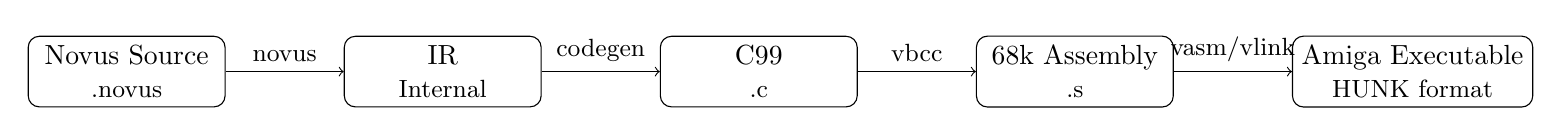
\begin{tikzpicture}[node distance=1.5cm, auto,
    box/.style={rectangle, draw, rounded corners, minimum width=2.5cm, minimum height=0.8cm, align=center}]
    \node[box] (novus) {Novus Source\\{\small .novus}};
    \node[box, right=of novus] (ir) {IR\\{\small Internal}};
    \node[box, right=of ir] (c) {C99\\{\small .c}};
    \node[box, right=of c] (asm) {68k Assembly\\{\small .s}};
    \node[box, right=of asm] (exe) {Amiga Executable\\{\small HUNK format}};

    \draw[->] (novus) -- node[above] {\small novus} (ir);
    \draw[->] (ir) -- node[above] {\small codegen} (c);
    \draw[->] (c) -- node[above] {\small vbcc} (asm);
    \draw[->] (asm) -- node[above] {\small vasm/vlink} (exe);
\end{tikzpicture}
\end{center}

\begin{enumerate}
    \item \textbf{Novus Compiler}: Parses your source, performs type checking, generates intermediate representation (IR)
    \item \textbf{Code Generation}: Converts IR to clean, readable C99 code
    \item \textbf{VBCC}: Compiles C to optimized 68k assembly
    \item \textbf{VASM/VLINK}: Assembles and links into an AmigaOS HUNK executable
\end{enumerate}

You can examine any stage:

\begin{lstlisting}[style=bash]
# Emit IR to see the compiler's internal representation
novus compile myfile.novus -o out --emit-ir

# Emit assembly to see exactly what instructions are generated
novus compile myfile.novus -o out --emit-asm
\end{lstlisting}

\subsection{Key Characteristics}

\begin{description}
    \item[Native Performance] Novus transpiles to C99, leveraging VBCC's mature 68k code generator to produce Amiga executables. There is no interpreter, no virtual machine, no runtime overhead beyond what you explicitly request.

    \item[Modern Safety] The type system catches errors at compile time. \texttt{Result} and \texttt{Option} types make error handling explicit. Resource cleanup is deterministic via the \texttt{Drop} trait and \texttt{defer} blocks. You get safety without garbage collection.

    \item[Direct Hardware Access] Novus doesn't hide the Amiga's hardware behind abstractions you can't escape. Custom chip registers, Exec library calls, copper lists, blitter operations---all are first-class citizens with typed, safe interfaces.

    \item[Readable Output] The generated C code is clean and readable. When you need to understand what the compiler is doing---and on the Amiga, you often do---the output won't fight you.

    \item[Amiga-Native Async] The \texttt{async}/\texttt{await} model maps directly to AmigaOS primitives: Exec signals and message ports. No hidden threads, no runtime scheduler---just the OS facilities the Amiga provides.
\end{description}

\subsection{A First Comparison}

Here's a simple function that opens a file and reads its size. First, the C version:

\begin{lstlisting}[language=C]
// C: Opening a file and getting its size
LONG get_file_size(const char *path) {
    BPTR lock = Lock(path, ACCESS_READ);
    if (!lock) {
        return -1;  // Caller must check return value!
    }

    struct FileInfoBlock *fib = AllocMem(sizeof(struct FileInfoBlock),
                                         MEMF_PUBLIC);
    if (!fib) {
        UnLock(lock);  // Must remember to clean up!
        return -1;
    }

    LONG size = -1;
    if (Examine(lock, fib)) {
        size = fib->fib_Size;
    }

    FreeMem(fib, sizeof(struct FileInfoBlock));  // Must match size!
    UnLock(lock);  // Must remember cleanup order!
    return size;
}
\end{lstlisting}

Now the same function in Novus:

\begin{lstlisting}
// Novus: Opening a file and getting its size
fn get_file_size(path: &str) -> Result<i32, DosError> {
    let lock = Lock::new(path, ACCESS_READ)?  // ? propagates errors
    let fib = FileInfoBlock::alloc()?

    lock.examine(&fib)?
    return Result::Ok(fib.size())
}  // lock and fib automatically cleaned up via Drop
\end{lstlisting}

The Novus version is shorter, but more importantly:

\begin{itemize}
    \item The return type \texttt{Result<i32, DosError>} makes failure explicit---callers \emph{must} handle it
    \item The \texttt{?} operator propagates errors automatically, no forgotten checks
    \item Resources are cleaned up automatically when they go out of scope
    \item No size mismatches possible---\texttt{FileInfoBlock} knows its own size
\end{itemize}

\begin{comingfromc}
In C, every function that can fail returns a value that might be an error. You must remember to check it. You must remember to clean up. You must match every allocation size.

In Novus, the type system enforces these rules. A \texttt{Result} \emph{must} be handled. Resources with \texttt{Drop} \emph{will} be cleaned up. The compiler tracks sizes for you.
\end{comingfromc}

\section{Why Novus Exists}

The Amiga platform has capable C compilers. VBCC, in particular, generates excellent code and remains actively maintained. So why create a new language?

\subsection{The Limits of C}

C was revolutionary in 1972. It remains useful today precisely because it's minimal---a portable assembler that gets out of your way. But that minimalism has costs:

\begin{itemize}
    \item \textbf{No sum types.} Representing ``this value is either an error or a result'' requires conventions that the compiler can't enforce.

    \item \textbf{No built-in error handling.} Return codes are easily ignored. Exceptions don't exist. Every function call is an opportunity for silent failure.

    \item \textbf{Manual resource management.} Matching every \texttt{AllocMem} with a \texttt{FreeMem}, every \texttt{OpenLibrary} with a \texttt{CloseLibrary}, every \texttt{Lock} with an \texttt{UnLock}---across all control flow paths, including error cases.

    \item \textbf{Primitive module system.} Header files and \texttt{\#include} are textual substitution. Name collisions, include order dependencies, and compile time explosion are facts of life.

    \item \textbf{No metaprogramming.} The preprocessor is powerful but crude. Anything beyond simple macros quickly becomes write-only code.
\end{itemize}

\subsection{Real Bugs from Real Software}

These aren't theoretical concerns. They're the source of real bugs in real Amiga software:

\textbf{The Forgotten \texttt{UnLock}:}
\begin{lstlisting}[language=C]
BOOL check_file(const char *path) {
    BPTR lock = Lock(path, ACCESS_READ);
    if (!lock) return FALSE;

    struct FileInfoBlock fib;
    if (!Examine(lock, &fib)) {
        return FALSE;  // BUG: lock leaked!
    }

    UnLock(lock);
    return TRUE;
}
\end{lstlisting}

Every early return is an opportunity to forget cleanup. In a large function with multiple resources, the combinations explode.

\textbf{The Ignored Return Value:}
\begin{lstlisting}[language=C]
void process_data(void) {
    Open("output.dat", MODE_NEWFILE);  // BUG: return value ignored!
    Write(file, data, size);           // file is uninitialized
}
\end{lstlisting}

C happily compiles this. The result: random corruption.

\textbf{The Mismatched Size:}
\begin{lstlisting}[language=C]
struct MyData *data = AllocMem(sizeof(struct MyData), MEMF_PUBLIC);
// ... 500 lines later, after the struct changed ...
FreeMem(data, sizeof(struct OtherData));  // BUG: wrong size!
\end{lstlisting}

Memory corruption. Guru meditation. Hours of debugging.

\subsection{How Novus Prevents These Bugs}

Each of these bugs is impossible in Novus:

\textbf{The Forgotten \texttt{UnLock}:}
\begin{lstlisting}
fn check_file(path: &str) -> Result<bool, DosError> {
    let lock = Lock::new(path, ACCESS_READ)?

    let fib = FileInfoBlock::alloc()?
    lock.examine(&fib)?

    return Result::Ok(true)
}  // lock.drop() called automatically on ALL paths
\end{lstlisting}

\textbf{The Ignored Return Value:}
\begin{lstlisting}
fn process_data() -> Result<(), DosError> {
    // This won't compile - Result must be handled:
    // let _ = open("output.dat", MODE_NEWFILE)  // Error: unused Result

    let file = open("output.dat", MODE_NEWFILE)?  // Must use ? or match
    write(&file, data, size)?
    return Result::Ok(())
}
\end{lstlisting}

\textbf{The Mismatched Size:}
\begin{lstlisting}
fn allocate_data() -> Result<Allocation<MyData>, ExecError> {
    let data = Allocation::<MyData>::alloc(MEMF_PUBLIC)?
    return Result::Ok(data)
}  // data.drop() frees with correct size automatically
\end{lstlisting}

\subsection{Modern Solutions, Amiga Constraints}

Languages like Rust address these problems elegantly. But Rust targets modern systems with megabytes of RAM, gigahertz CPUs, and operating systems that provide virtual memory and threads. Its runtime assumptions don't map to the Amiga.

Novus takes a different approach: provide modern ergonomics within Amiga constraints.

\begin{itemize}
    \item \texttt{Result<T, E>} and \texttt{Option<T>} are zero-cost at runtime---they're just tagged unions that the compiler understands.

    \item The \texttt{Drop} trait compiles to cleanup code inserted at scope exit. No hidden allocations, no unwinding tables.

    \item Pattern matching compiles to efficient jump tables or comparison chains as appropriate.

    \item The module system is compile-time only. No runtime symbol resolution, no dynamic linking overhead.

    \item Fixed-point math uses inline 68020+ instructions, not floating-point emulation.
\end{itemize}

The result is a language that \emph{feels} modern but \emph{runs} like hand-tuned assembly.

\section{Design Philosophy}

Novus follows several core principles that inform every language decision.

\subsection{Explicit Over Implicit}

If something allocates memory, the code should say so. If something can fail, the type should reflect it. If a function has side effects, they should be visible at the call site.

\begin{lstlisting}
// Allocation is explicit - you know this allocates
var buffer = MemoryBlock::alloc(1024, MEMF_CHIP)?

// Failure is explicit - Result type, can't ignore
let file = open("data.dat", MODE_OLDFILE)?

// Mutation is explicit at the call site
process(&var player)  // Clearly modifying player
\end{lstlisting}

This doesn't mean verbose---Novus has type inference, sensible defaults, and concise syntax. But it means no hidden costs, no action at a distance, no ``magic'' that obscures what the machine is actually doing.

\begin{comingfromc}
In C, \texttt{process(player)} might modify \texttt{player} or it might not---you have to read the function signature.

In Novus, \texttt{process(\&player)} is read-only. \texttt{process(\&var player)} mutates. The call site tells you.
\end{comingfromc}

\subsection{Predictable Performance}

On a 7~MHz 68000, every cycle matters. On a 50~MHz 68060, you have more headroom---but you still can't afford hidden allocations in a tight loop or cache-hostile memory access patterns.

Novus gives you control. The compiler won't secretly box values, won't insert invisible runtime checks in release builds, won't generate code that's impossible to reason about.

Consider this function:

\begin{lstlisting}
fn sum_array(data: &[i32]) -> i32 {
    var total: i32 = 0
    for value in data {
        total = total + value
    }
    return total
}
\end{lstlisting}

The generated 68k assembly is exactly what you'd expect:

\begin{lstlisting}[style=bash]
sum_array:
    moveq   #0,d0           ; total = 0
    move.l  d2,-(sp)        ; save d2
    move.l  (a0),d2         ; d2 = slice length
    addq.l  #4,a0           ; a0 = data pointer
.loop:
    subq.l  #1,d2           ; decrement counter
    bmi.s   .done           ; done if negative
    add.l   (a0)+,d0        ; total += *data++
    bra.s   .loop
.done:
    move.l  (sp)+,d2        ; restore d2
    rts
\end{lstlisting}

No hidden function calls. No allocations. Just a tight loop.

\subsection{Respect the Machine}

The Amiga isn't a Unix workstation. It has custom chips that do things no other hardware can do. Its operating system uses message passing and signals, not files and processes. Its memory model is flat and physical.

Novus doesn't pretend otherwise. The standard library wraps AmigaOS idiomatically---\texttt{Result} types for operations that can fail, handles for resources that need cleanup---but it doesn't try to be POSIX. Amiga code should look like Amiga code.

\begin{lstlisting}
// Copper lists, typed and safe
var builder = CopperListBuilder::new()
builder.wait(100, 0)?
builder.move_color(0, rgb12(15, 0, 0))?  // Set background red
let copper_list = builder.build()?
copper_list.activate()

// Blitter operations
blitter.blit_fill(&var bitmap, x, y, width, height, color)?

// Message ports for IPC
let port = MsgPort::create("myport")?
let signal = port.signal_bit()
let sigs = Wait(1 << signal)
\end{lstlisting}

\subsection{Fail Fast, Fail Clearly}

When something goes wrong, you should know immediately and know exactly what happened. Compile-time errors are better than runtime errors. Runtime errors with clear messages are better than silent corruption.

In debug builds, Novus checks array bounds, validates pointers, and panics with meaningful diagnostics:

\begin{lstlisting}[style=bash]
PANIC at src/player.novus:42
  Array index out of bounds: index 10, length 8

  Stack trace:
    update_score (src/player.novus:42)
    game_loop (src/main.novus:156)
    main (src/main.novus:12)
\end{lstlisting}

In release builds, those checks can be removed via \texttt{--safety-level}---but the type system still prevents the errors that checks would catch.

\section{A Taste of Novus}

Before diving into the full language, let's look at a complete program. This opens an Intuition window, draws a message, and waits for the user to close it:

\begin{lstlisting}
// hello_window.novus - A complete Novus program
from std::core import Result
from std::ffi::intuition import OpenWindowTags, CloseWindow
from std::ffi::graphics import SetAPen, Move, Text
from std::ffi::exec import Wait
from std::ffi::amiga_consts import (
    WA_Width, WA_Height, WA_Title, WA_Flags, WA_IDCMP,
    WFLG_CLOSEGADGET, WFLG_DRAGBAR, WFLG_ACTIVATE,
    IDCMP_CLOSEWINDOW, TAG_DONE
)

pub fn main() -> i32 {
    // Open a window with the close gadget
    var window: *Window = null

    unsafe {
        window = OpenWindowTags(null,
            WA_Width, 320,
            WA_Height, 100,
            WA_Title, "Hello from Novus!",
            WA_Flags, WFLG_CLOSEGADGET | WFLG_DRAGBAR | WFLG_ACTIVATE,
            WA_IDCMP, IDCMP_CLOSEWINDOW,
            TAG_DONE)
    }

    if window == null {
        return 1  // Window open failed
    }

    // Draw text in the window
    unsafe {
        let rp = window.RPort
        SetAPen(rp, 1)           // Color 1 (usually white)
        Move(rp, 20, 50)         // Position cursor
        Text(rp, "Welcome to Novus!", 17)
    }

    // Wait for close gadget
    unsafe {
        let signal = 1u32 << window.UserPort.mp_SigBit
        Wait(signal)
    }

    // Clean up
    unsafe {
        CloseWindow(window)
    }

    return 0
}
\end{lstlisting}

This is deliberately written in ``raw'' style, calling AmigaOS functions directly with \texttt{unsafe} blocks. Later chapters show the safer stdlib wrappers, but this demonstrates that Novus gives you full access to the platform.

\begin{comingfromc}
Notice what's different from C:
\begin{itemize}
    \item No \texttt{\#include} files---\texttt{from...import} brings in what you need
    \item No semicolons required (they're optional)
    \item \texttt{null} instead of \texttt{NULL}
    \item \texttt{unsafe \{\}} blocks mark where you're bypassing safety checks
    \item Return type comes after the function name: \texttt{fn main() -> i32}
\end{itemize}

What's the same:
\begin{itemize}
    \item Same AmigaOS functions: \texttt{OpenWindowTags}, \texttt{Wait}, etc.
    \item Same structures: \texttt{Window}, \texttt{RastPort}
    \item Same constants: \texttt{WA\_Width}, \texttt{IDCMP\_CLOSEWINDOW}
    \item Same calling convention and memory layout
\end{itemize}
\end{comingfromc}

\section{What Novus Doesn't Do}

Honesty about limitations helps you make informed decisions. Novus is not a general-purpose language. It's designed for Amiga development, and it makes trade-offs accordingly.

\subsection{No Garbage Collection}

Novus uses deterministic resource management via RAII (the \texttt{Drop} trait). When a value goes out of scope, its destructor runs immediately. This is predictable and has zero overhead---but it means you must think about ownership.

Cyclic data structures require extra care. Reference counting (via \texttt{Rc<T>}) is available when needed, but it's explicit, not automatic.

\subsection{No Exceptions}

Error handling uses \texttt{Result<T, E>} and the \texttt{?} operator, not exceptions. This means:

\begin{itemize}
    \item No invisible control flow jumps
    \item No unwinding tables taking up code space
    \item Errors are always visible in function signatures
\end{itemize}

But it also means you can't \texttt{catch} an error from deep in a call stack without propagating it explicitly through each level.

\subsection{No Hidden Threads}

The Amiga's multitasking is cooperative and explicit. Novus's \texttt{async}/\texttt{await} compiles to state machines driven by Exec signals---there's no hidden thread pool, no automatic parallelism.

If you want parallel execution, you create Exec tasks explicitly. Novus gives you tools to do this safely, but it doesn't do it behind your back.

\subsection{68020 Minimum}

Novus targets 68020+ processors. The 68000/68010 lacks instructions that the compiler relies on (32-bit multiply/divide, bitfield operations). If you're targeting a stock A500 or A1000, Novus isn't the right choice---use C with VBCC directly.

This isn't a significant limitation in practice. Most Amiga users have accelerators, and the A1200/A4000 shipped with 68020/68040.

\section{Target Audience}

This guide assumes you're a working programmer. You should be comfortable with:

\begin{itemize}
    \item Systems programming concepts: pointers, memory allocation, stack vs. heap
    \item Basic 68k architecture: registers, addressing modes, the supervisor/user split
    \item AmigaOS fundamentals: libraries, Exec, DOS, the message-passing model
\end{itemize}

Prior experience with Rust, Swift, or other modern systems languages will make Novus feel familiar, but it's not required. If you've written C for the Amiga, you have all the background you need.

\section{How to Read This Guide}

The guide is organized in layers:

\begin{description}
    \item[Part I: Language Fundamentals] covers the core language---syntax, types, control flow, functions, and modules. Read this first.

    \item[Part II: Standard Library] documents the \texttt{std} packages: collections, strings, memory management, and Amiga OS bindings.

    \item[Part III: Advanced Topics] covers async programming, inline assembly, FFI with existing C code, and performance optimization.

    \item[Appendices] provide quick references, grammar summaries, and migration guides from C.
\end{description}

Code examples are designed to be complete and runnable. When a snippet requires context, we provide it. When we omit boilerplate, we say so.

\section{Showcase: Copper Rainbow}

To close this introduction, here's a program that demonstrates what makes Novus special for Amiga development. It uses the copper coprocessor to create a smooth rainbow gradient across the screen---something that would be impossible on any other platform.

\begin{lstlisting}
// copper_rainbow.novus - A visual showcase
from std::core import Result
from std::graphics::copper import CopperListBuilder, CopperListHandle, CopperError
from std::hardware::registers import rgb12
from std::os::timer import delay, Duration
from std::ffi::graphics import WaitTOF

/// Interpolate between two colors
fn lerp_color(c1: u16, c2: u16, t: u16) -> u16 {
    let r1 = (c1 >> 8) & $F
    let r2 = (c2 >> 8) & $F
    let g1 = (c1 >> 4) & $F
    let g2 = (c2 >> 4) & $F
    let b1 = c1 & $F
    let b2 = c2 & $F

    let r = r1 + ((r2 - r1) * t) / 256
    let g = g1 + ((g2 - g1) * t) / 256
    let b = b1 + ((b2 - b1) * t) / 256

    return rgb12((u8)r, (u8)g, (u8)b)
}

/// Get rainbow color for position 0-255
fn rainbow(pos: u8) -> u16 {
    let p = (u16)pos
    let segment = p / 43
    let offset = (p % 43) * 6

    match segment {
        0 => lerp_color(rgb12(15,0,0), rgb12(15,15,0), offset),
        1 => lerp_color(rgb12(15,15,0), rgb12(0,15,0), offset),
        2 => lerp_color(rgb12(0,15,0), rgb12(0,15,15), offset),
        3 => lerp_color(rgb12(0,15,15), rgb12(0,0,15), offset),
        4 => lerp_color(rgb12(0,0,15), rgb12(15,0,15), offset),
        _ => lerp_color(rgb12(15,0,15), rgb12(15,0,0), offset),
    }
}

/// Build copper list with rainbow gradient
fn build_rainbow() -> Result<CopperListHandle, CopperError> {
    var builder = CopperListBuilder::new()

    var line: u16 = 0
    while line < 200 {
        let scanline = 44 + line
        let color_pos = (line * 256) / 200
        let color = rainbow((u8)color_pos)

        builder.wait(scanline, 0)?
        builder.move_color(0, color)?

        line = line + 2
    }

    builder.wait(244, 0)?
    builder.move_color(0, rgb12(0, 0, 0))?

    return builder.build()
}

pub fn main() -> i32 {
    unsafe { WaitTOF() }

    match build_rainbow() {
        Result::Ok(copper_list) => {
            unsafe { copper_list.activate() }
            let _ = delay(Duration::secs(5))
            return 0  // Copper list cleaned up by Drop
        },
        Result::Err(_) => return 1
    }
}
\end{lstlisting}

This 70-line program:

\begin{itemize}
    \item Uses \texttt{Result} for error handling throughout
    \item Relies on RAII---the copper list restores the display when dropped
    \item Talks directly to the copper hardware through safe abstractions
    \item Compiles to tight, efficient 68k code
\end{itemize}

Run it on real hardware or in FS-UAE to see a smooth, colorful gradient scroll across your screen. This is what Novus is for: making the Amiga's unique capabilities accessible with modern safety and ergonomics.

Let's begin.

\chapter{Getting Started}
\label{ch:getting-started}

\begin{quote}
\textit{``The journey of a thousand miles begins with a single step.''}\\
---Lao Tzu
\end{quote}

\vspace{1em}

This chapter walks you through installing the Novus compiler, writing your first program, and understanding the compilation pipeline. By the end, you'll have a working executable running on your Amiga (or emulator).

% ============================================================================
\section{Quick Start}
\label{sec:quick-start}
% ============================================================================

If you already have Novus installed, here's the fastest path to ``Hello, Amiga!'':

\begin{enumerate}
\item Create \texttt{hello.novus}:
\begin{lstlisting}
from std::io::file import println

pub fn main() -> i32 {
    println("Hello, Amiga!")
    return 0
}
\end{lstlisting}

\item Compile:
\begin{lstlisting}[language=bash]
novus compile hello.novus -o hello
\end{lstlisting}

\item Copy to your Amiga and run:
\begin{lstlisting}[language=bash]
1.Workbench:> hello
Hello, Amiga!
\end{lstlisting}
\end{enumerate}

That's it! The rest of this chapter explains the prerequisites, installation, and toolchain in detail.

% ============================================================================
\section{Prerequisites}
\label{sec:prerequisites}
% ============================================================================

Before installing Novus, ensure you have:

\begin{itemize}
    \item \textbf{.NET 9.0 or later} --- The Novus compiler is written in C\# and requires the .NET runtime. Download from \texttt{https://dotnet.microsoft.com}

    \item \textbf{VBCC toolchain} --- Novus uses VBCC's assembler (\texttt{vasmm68k\_mot}) and linker (\texttt{vlink}) to produce Amiga executables. The toolchain is vendored in the repository under \texttt{vendor/vbcc}, or you can specify a custom installation via the \texttt{--vbcc-path} option.

    \item \textbf{An Amiga or emulator} --- To run your compiled programs. FS-UAE, WinUAE, or real hardware all work. A 68020+ configuration with AmigaOS 2.0 or later is required.
\end{itemize}

% ============================================================================
\section{Installation}
\label{sec:installation}
% ============================================================================

\subsection{Platform-Specific Instructions}

\subsubsection{macOS}

\begin{enumerate}
\item Install .NET SDK using Homebrew:
\begin{lstlisting}[language=bash]
brew install dotnet
\end{lstlisting}

\item Clone and build Novus:
\begin{lstlisting}[language=bash]
git clone https://github.com/barryw/Novus.git
cd Novus
dotnet build
\end{lstlisting}

\item Add to your PATH (optional):
\begin{lstlisting}[language=bash]
export PATH="$PATH:$(pwd)/Novus/bin/Debug/net9.0"
\end{lstlisting}
\end{enumerate}

\subsubsection{Linux}

\begin{enumerate}
\item Install .NET SDK:
\begin{lstlisting}[language=bash]
# Ubuntu/Debian
sudo apt install dotnet-sdk-9.0

# Fedora
sudo dnf install dotnet-sdk-9.0
\end{lstlisting}

\item Clone and build:
\begin{lstlisting}[language=bash]
git clone https://github.com/barryw/Novus.git
cd Novus
dotnet build
\end{lstlisting}
\end{enumerate}

\subsubsection{Windows}

\begin{enumerate}
\item Download and install .NET SDK from \texttt{https://dotnet.microsoft.com}

\item Clone the repository (using Git Bash, PowerShell, or WSL):
\begin{lstlisting}[language=bash]
git clone https://github.com/barryw/Novus.git
cd Novus
dotnet build
\end{lstlisting}
\end{enumerate}

\textbf{WSL Note:} If you prefer Linux tools, Windows Subsystem for Linux works well. Install the Linux .NET SDK inside WSL and compile there.

\subsection{Verifying Installation}

After building, verify everything works:

\begin{lstlisting}[language=bash]
# Check the Novus compiler
./Novus/bin/Debug/net9.0/novus --version

# Check VBCC tools (vendored)
./vendor/vbcc/bin/vasm --version 2>&1 | head -1
./vendor/vbcc/bin/vlink --version 2>&1 | head -1
\end{lstlisting}

You should see version information for each tool.

\subsection{Troubleshooting}

\textbf{Problem:} \texttt{dotnet: command not found}\\
\textbf{Solution:} .NET SDK is not installed or not in PATH. Reinstall and ensure the install location is in your PATH.

\textbf{Problem:} \texttt{VBCC tools not found}\\
\textbf{Solution:} The vendored VBCC is under \texttt{vendor/vbcc}. If using a custom VBCC installation, pass \texttt{--vbcc-path /path/to/vbcc} to the compiler.

\textbf{Problem:} Build fails with missing dependencies\\
\textbf{Solution:} Run \texttt{dotnet restore} to fetch NuGet packages.

\begin{comingfromc}
Setting up a C cross-compiler for Amiga traditionally involves:
\begin{enumerate}
\item Downloading VBCC, vasm, and vlink separately
\item Setting \texttt{VBCC} environment variable
\item Creating \texttt{vc.config} with include/library paths
\item Finding and installing the AmigaOS NDK
\item Setting up include paths for system headers
\end{enumerate}

Novus bundles everything in the repository---no environment variables or configuration files needed. Just \texttt{dotnet build} and compile.
\end{comingfromc}

% ============================================================================
\section{Your First Program}
\label{sec:first-program}
% ============================================================================

Create a file named \texttt{hello.novus}:

\begin{lstlisting}
from std::io::file import println

pub fn main() -> i32 {
    println("Hello, Amiga!")
    return 0
}
\end{lstlisting}

\subsection{Line-by-Line Explanation}

\textbf{Line 1: \texttt{from std::io::file import println}}

This imports the \texttt{println} function from the standard library's I/O module. Unlike some languages where printing is built-in, Novus requires explicit imports. This keeps the language core small and makes dependencies visible.

\texttt{std::io::file} is the module path:
\begin{itemize}
    \item \texttt{std} --- the standard library
    \item \texttt{io} --- the I/O subsystem
    \item \texttt{file} --- file and console operations
\end{itemize}

\textbf{Line 3: \texttt{pub fn main() -> i32}}

This declares the program entry point. Every Novus program must have exactly one \texttt{main} function that:
\begin{itemize}
    \item Is marked \texttt{pub} (public) so the linker can find it
    \item Takes no parameters
    \item Returns \texttt{i32} --- the exit code passed back to AmigaOS
\end{itemize}

\textbf{Line 4: \texttt{println("Hello, Amiga!")}}

Calls the imported \texttt{println} function with a string literal. String literals in Novus are null-terminated C-style strings (\texttt{*u8}).

\textbf{Line 5: \texttt{return 0}}

Returns the exit code. Zero means success; non-zero indicates an error. AmigaOS and the Shell use this to detect failures.

\subsection{Compiling}

Compile to an Amiga executable:

\begin{lstlisting}[language=bash]
novus compile hello.novus -o hello
\end{lstlisting}

This produces an executable named \texttt{hello} in Amiga HUNK format. Without the \texttt{-o} flag, the output defaults to \texttt{a.out}.

\subsection{What Happens During Compilation}

When you compile, Novus performs these steps:

\begin{enumerate}
\item \textbf{Parse} --- Read \texttt{hello.novus} and build an AST
\item \textbf{Analyze} --- Check types, resolve names, build IR
\item \textbf{Import} --- Load \texttt{std::io::file} and its dependencies
\item \textbf{Generate} --- Emit C99 code for your program and used stdlib functions
\item \textbf{Compile} --- VBCC compiles C to 68k object files
\item \textbf{Link} --- vlink combines objects into a HUNK executable
\end{enumerate}

Use \texttt{-v} (verbose) to watch this process:

\begin{lstlisting}[language=bash]
novus compile hello.novus -o hello -v
\end{lstlisting}

\subsection{Running on the Amiga}

Transfer the executable to your Amiga and run it from the Shell:

\begin{lstlisting}[language=bash]
1.Workbench:> hello
Hello, Amiga!
\end{lstlisting}

Congratulations---you've run your first Novus program!

% ============================================================================
\section{A More Complete Example}
\label{sec:complete-example}
% ============================================================================

Let's look at a program that does more than print a message. This example queries and displays system memory information:

\begin{lstlisting}
// memory_info.novus - Display memory statistics
from std::io::file import print, println
from std::ffi::exec import AvailMem
from std::ffi::amiga_consts import MEMF_CHIP, MEMF_FAST, MEMF_TOTAL

pub fn main() -> i32 {
    println("Memory Information")
    println("==================")

    // Query chip RAM (DMA-accessible memory)
    let chip_mem = unsafe { AvailMem(MEMF_CHIP | MEMF_TOTAL) }

    // Query fast RAM (CPU-only memory)
    let fast_mem = unsafe { AvailMem(MEMF_FAST | MEMF_TOTAL) }

    // Display results
    print("Chip RAM: ")
    print_kb(chip_mem)
    println(" KB")

    print("Fast RAM: ")
    print_kb(fast_mem)
    println(" KB")

    print("Total:    ")
    print_kb(chip_mem + fast_mem)
    println(" KB")

    return 0
}

fn print_kb(bytes: u32) {
    let kb = bytes / 1024u32
    print_number(kb)
}

fn print_number(n: u32) {
    if n == 0 { return }
    if n >= 10 { print_number(n / 10u32) }
    let digit: u8 = (u8)(n % 10u32) + 48u8
    var buf = [0u8; 2]
    buf[0] = digit
    print(&buf[0])
}
\end{lstlisting}

This example demonstrates:
\begin{itemize}
    \item \textbf{Multiple imports} from different modules
    \item \textbf{Unsafe FFI calls} to AmigaOS via \texttt{AvailMem}
    \item \textbf{Constants} like \texttt{MEMF\_CHIP} from the FFI layer
    \item \textbf{Helper functions} for formatting output
    \item \textbf{Arithmetic and type casts}
\end{itemize}

\begin{comingfromc}
The equivalent C code would look similar, but you'd need to:
\begin{itemize}
    \item Include \texttt{<proto/exec.h>} or set up function prototypes
    \item Link with \texttt{amiga.lib} or use direct library calls
    \item Deal with library bases (\texttt{SysBase})
\end{itemize}

In Novus, the FFI layer handles library opening/closing automatically. Just import and call.
\end{comingfromc}

% ============================================================================
\section{The Compilation Pipeline}
\label{sec:compilation-pipeline}
% ============================================================================

Understanding the compilation pipeline helps with debugging and optimization. Here's what happens when you compile:

% TikZ diagram of compilation pipeline
\begin{center}
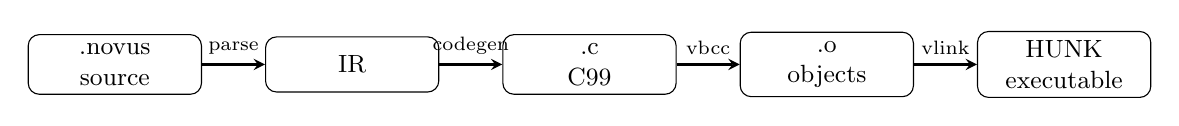
\begin{tikzpicture}[
    node distance=0.8cm,
    box/.style={rectangle, draw, rounded corners, minimum width=2.2cm, minimum height=0.7cm, align=center, font=\small},
    arrow/.style={->, >=stealth, thick}
]
    \node[box] (source) {.novus\\source};
    \node[box, right=of source] (ir) {IR};
    \node[box, right=of ir] (c) {.c\\C99};
    \node[box, right=of c] (obj) {.o\\objects};
    \node[box, right=of obj] (exe) {HUNK\\executable};

    \draw[arrow] (source) -- node[above, font=\scriptsize] {parse} (ir);
    \draw[arrow] (ir) -- node[above, font=\scriptsize] {codegen} (c);
    \draw[arrow] (c) -- node[above, font=\scriptsize] {vbcc} (obj);
    \draw[arrow] (obj) -- node[above, font=\scriptsize] {vlink} (exe);
\end{tikzpicture}
\end{center}

\subsection{Stage 1: Parsing and Analysis}

The Novus compiler reads your source file, parses it into an Abstract Syntax Tree (AST), then performs semantic analysis:
\begin{itemize}
    \item Type checking
    \item Name resolution
    \item Trait resolution
    \item Building the Intermediate Representation (IR)
\end{itemize}

Use \texttt{--emit-ir} to see the IR:

\begin{lstlisting}[language=bash]
novus compile hello.novus --emit-ir
\end{lstlisting}

\subsection{Stage 2: C Code Generation}

The IR is lowered to C99 code. Each function becomes a C function; each type becomes a C struct or typedef. The generated C uses VBCC-specific extensions for 68k calling conventions.

\subsection{Stage 3: Object File Compilation}

VBCC's C compiler (\texttt{vbccm68k}) compiles the C code to 68k object files. Each function is compiled separately for incremental builds.

Use \texttt{--emit-asm} to see the generated assembly:

\begin{lstlisting}[language=bash]
novus compile hello.novus --emit-asm
\end{lstlisting}

This is useful for understanding performance characteristics or debugging codegen issues.

\subsection{Stage 4: Linking}

\texttt{vlink} combines all object files---your code, the runtime, and stdlib---into a final executable in Amiga HUNK format. Dead code elimination removes unused functions to keep binaries small.

% ============================================================================
\section{Development Workflow}
\label{sec:dev-workflow}
% ============================================================================

\subsection{Fast Feedback with novus check}

For quick syntax and type checking without full compilation:

\begin{lstlisting}[language=bash]
novus check myfile.novus
\end{lstlisting}

This skips code generation and linking, giving faster feedback during development.

\subsection{Code Formatting}

Keep your code consistent with \texttt{novus fmt}:

\begin{lstlisting}[language=bash]
novus fmt myfile.novus
\end{lstlisting}

This reformats the file in place according to the Novus style guide.

\subsection{Editor Support}

Novus provides a Language Server Protocol (LSP) implementation for IDE integration:
\begin{itemize}
    \item \textbf{VS Code} --- Install the Novus extension from the marketplace
    \item \textbf{Other editors} --- Configure your LSP client to use \texttt{novus lsp}
\end{itemize}

Features include:
\begin{itemize}
    \item Syntax highlighting
    \item Error diagnostics as you type
    \item Go to definition
    \item Hover information
    \item Code completion
\end{itemize}

% ============================================================================
\section{Running on Real Hardware}
\label{sec:real-hardware}
% ============================================================================

The ultimate goal is running on real Amiga hardware. Here are several ways to transfer executables.

\subsection{Shared Folders (Emulator)}

If using FS-UAE, WinUAE, or Amiberry, configure a shared folder:

\begin{enumerate}
\item Create a directory on your host system (e.g., \texttt{\textasciitilde/amiga\_share})
\item Configure the emulator to mount it as a device (e.g., \texttt{DEV:})
\item Compile directly to the shared folder:
\begin{lstlisting}[language=bash]
novus compile hello.novus -o ~/amiga_share/hello
\end{lstlisting}
\item Access from the Amiga: \texttt{DEV:hello}
\end{enumerate}

\subsection{Network Transfer}

With networked Amigas (via Plipbox, A2065, or similar):

\begin{lstlisting}[language=bash]
# Using scp (requires AmiSSH or similar on the Amiga)
scp hello amiga.local:Work/

# Using ftp
ftp amiga.local
put hello
\end{lstlisting}

\subsection{CF/SD Card}

For accelerator cards with CF/SD storage:

\begin{enumerate}
\item Mount the card on your development machine
\item Copy the executable to the card
\item Unmount and return the card to the Amiga
\end{enumerate}

\subsection{Floppy Disk Images}

Create an ADF image with your executable:

\begin{lstlisting}[language=bash]
# Create a new ADF
xdftool myfiles.adf format "MyDisk" + write hello
\end{lstlisting}

Then use the ADF in your emulator or write it to a real floppy.

% ============================================================================
\section{Project Structure}
\label{sec:project-structure}
% ============================================================================

For anything beyond a single file, create a project with \texttt{novus new}:

\begin{lstlisting}[language=bash]
novus new myproject --type cli
cd myproject
\end{lstlisting}

This creates a standard project structure:

\begin{lstlisting}[language=bash]
myproject/
    project.toml        # Project configuration
    src/
        main.novus      # Entry point
\end{lstlisting}

\subsection{The project.toml File}

The \texttt{project.toml} file defines project metadata and build settings:

\begin{lstlisting}
[package]
name = "myproject"
version = "0.1.0"
authors = ["Your Name"]
description = "My first Novus project"

[build]
target_cpu = "68020"
fpu = "auto"
optimization_level = 0
output = "build"
\end{lstlisting}

\subsection{Build Settings Reference}

\begin{center}
\begin{tabular}{llp{6cm}}
\textbf{Setting} & \textbf{Default} & \textbf{Description} \\
\hline
\texttt{target\_cpu} & \texttt{auto} & Target CPU: 68020, 68030, 68040, 68060, or auto \\
\texttt{fpu} & \texttt{auto} & FPU mode: soft, 68881, 68040, or auto \\
\texttt{optimization\_level} & \texttt{0} & VBCC optimization level (0--3) \\
\texttt{output} & \texttt{build} & Output directory for compiled files \\
\texttt{stack\_size} & \texttt{4096} & Stack size in bytes \\
\end{tabular}
\end{center}

Build the project with:

\begin{lstlisting}[language=bash]
novus build
\end{lstlisting}

% ============================================================================
\section{Compiler Commands Reference}
\label{sec:commands}
% ============================================================================

\begin{description}
    \item[\texttt{novus compile <file>}] Compile a single source file to an executable
    \item[\texttt{novus build}] Build a project defined by \texttt{project.toml}
    \item[\texttt{novus check <file>}] Type-check without generating code
    \item[\texttt{novus test <file>}] Compile test runner
    \item[\texttt{novus new <name>}] Create a new project from a template
    \item[\texttt{novus fmt <file>}] Format source code
    \item[\texttt{novus clean}] Remove cached build artifacts
    \item[\texttt{novus lsp}] Start the language server
\end{description}

\subsection{Common Options}

Options for \texttt{novus compile}:

\begin{description}
    \item[\texttt{-o, --output}] Output file name (default: \texttt{a.out})
    \item[\texttt{--cpu}] Target CPU: \texttt{68020}, \texttt{68030}, \texttt{68040}, \texttt{68060}, or \texttt{auto}
    \item[\texttt{--fpu}] FPU mode: \texttt{soft}, \texttt{68881}, \texttt{68040}, or \texttt{auto}
    \item[\texttt{--release}] Enable optimizations and disable debug checks
    \item[\texttt{-O}] Optimization level (0--2)
    \item[\texttt{--emit-asm}] Emit assembly output only
    \item[\texttt{--emit-ir}] Emit IR to stdout
    \item[\texttt{-v, --verbose}] Show detailed progress
\end{description}

\subsection{Debug vs Release Builds}

By default, Novus compiles in debug mode:
\begin{itemize}
    \item Array bounds checking enabled
    \item Debug symbols included
    \item Minimal optimizations
\end{itemize}

For production, use \texttt{--release}:

\begin{lstlisting}[language=bash]
novus compile hello.novus -o hello --release
\end{lstlisting}

% ============================================================================
\section{The Standard Library}
\label{sec:stdlib}
% ============================================================================

Novus includes a comprehensive standard library:

\begin{description}
    \item[\texttt{std::core}] Fundamental types: \texttt{Option}, \texttt{Result}, core traits
    \item[\texttt{std::collections}] Data structures: \texttt{Vec}, \texttt{HashMap}, \texttt{HashSet}
    \item[\texttt{std::strings}] String handling: \texttt{String}, \texttt{Str}, \texttt{StringBuilder}
    \item[\texttt{std::memory}] Memory management, slices
    \item[\texttt{std::math}] Fixed-point arithmetic, trigonometry
    \item[\texttt{std::io}] File and console I/O
    \item[\texttt{std::ffi}] AmigaOS bindings (Exec, DOS, Graphics, Intuition)
    \item[\texttt{std::hardware}] CPU/chipset detection, memory info
\end{description}

Import with \texttt{from}:

\begin{lstlisting}
from std::collections::vec import Vec
from std::io::file import println
\end{lstlisting}

% ============================================================================
\section{Showcase: System Information}
\label{sec:showcase-sysinfo}
% ============================================================================

This program demonstrates the concepts from this chapter by querying and displaying system information:

\begin{lstlisting}
// sysinfo.novus - System Information Display
from std::core import Option
from std::io::file import print, println
from std::ffi::exec import AvailMem
from std::ffi::amiga_consts import MEMF_FAST, MEMF_CHIP
from std::ffi::amiga_consts import MEMF_TOTAL, MEMF_LARGEST

fn print_memory(label: *u8, bytes: u32) {
    print("  ")
    print(label)
    print(": ")
    let kb: u32 = bytes / 1024u32
    if kb == 0 {
        print("0")
    } else {
        print_number(kb)
    }
    println(" KB")
}

fn print_number(n: u32) {
    if n == 0 { return }
    if n >= 10 { print_number(n / 10u32) }
    let digit: u8 = (u8)(n % 10u32) + 48u8
    var buf = [0u8; 2]
    buf[0] = digit
    print(&buf[0])
}

fn show_memory_info() {
    println("")
    println("MEMORY")
    println("----------------------------------------")

    let chip_total = unsafe { AvailMem(MEMF_CHIP | MEMF_TOTAL) }
    let chip_largest = unsafe { AvailMem(MEMF_CHIP | MEMF_LARGEST) }
    print_memory("Chip RAM Total", chip_total)
    print_memory("Chip RAM Largest Block", chip_largest)

    println("")

    let fast_total = unsafe { AvailMem(MEMF_FAST | MEMF_TOTAL) }
    if fast_total > 0 {
        let fast_largest = unsafe { AvailMem(MEMF_FAST | MEMF_LARGEST) }
        print_memory("Fast RAM Total", fast_total)
        print_memory("Fast RAM Largest Block", fast_largest)
    } else {
        println("  Fast RAM: Not installed")
    }
}

pub fn main() -> i32 {
    println("============================================")
    println("         NOVUS SYSTEM INFORMATION")
    println("============================================")

    show_memory_info()

    println("")
    println("============================================")
    return 0
}
\end{lstlisting}

This program demonstrates:
\begin{itemize}
    \item \textbf{Imports} from multiple stdlib modules
    \item \textbf{Unsafe FFI calls} to \texttt{AvailMem}
    \item \textbf{Constants} from \texttt{amiga\_consts}
    \item \textbf{Helper functions} for output formatting
    \item \textbf{Control flow} with conditionals
\end{itemize}

The full source code is available in \texttt{Novus.Tests/Examples/sysinfo\_showcase.novus}.

% ============================================================================
\section{Running Tests}
\label{sec:running-tests}
% ============================================================================

Novus has built-in test support. Mark test functions with the \texttt{@test} attribute:

\begin{lstlisting}
from std::test::test import expect_eq

@test
fn test_addition() {
    expect_eq(2 + 2, 4, "basic addition")
}

@test
fn test_multiplication() {
    expect_eq(3 * 7, 21, "basic multiplication")
}
\end{lstlisting}

Compile the test runner:

\begin{lstlisting}[language=bash]
novus test mytest.novus
\end{lstlisting}

\textbf{Important:} The test command builds the test runner but does not execute it. Transfer the executable to your Amiga to run the tests.

% ============================================================================
\section{Next Steps}
\label{sec:next-steps}
% ============================================================================

You now have a working Novus installation and understand the basic workflow. The following chapters cover:

\begin{itemize}
    \item \textbf{Chapter~\ref{ch:basics}: Language Basics} --- Variables, types, and expressions
    \item \textbf{Chapter~\ref{ch:types}: Types} --- The type system in depth
    \item \textbf{Chapter~\ref{ch:memory}: Memory Management} --- Safe and explicit memory handling
    \item \textbf{Chapter~\ref{ch:control-flow}: Control Flow} --- Conditionals, loops, and pattern matching
\end{itemize}

When you're ready, turn the page and start learning the language itself.

\chapter{Language Basics}
\label{ch:basics}

\begin{quote}
\textit{``Simplicity is prerequisite for reliability.''}\\
---Edsger W. Dijkstra
\end{quote}

\vspace{1em}

This chapter covers the fundamental building blocks of Novus: how to declare variables, what types are available, how literals work, and how expressions combine values. By the end, you'll understand the core syntax and be ready to write meaningful programs.

\section{Comments}

Novus supports two comment styles:

\subsection{Single-Line Comments}

Use \texttt{//} for comments that extend to the end of the line:

\begin{lstlisting}
// This is a single-line comment
let x = 42  // Comments can appear after code
\end{lstlisting}

\subsection{Multi-Line Comments}

Use \texttt{/* */} for comments spanning multiple lines:

\begin{lstlisting}
/*
 * This is a multi-line comment.
 * Useful for longer explanations.
 */
let result = compute()
\end{lstlisting}

Multi-line comments do not nest. The first \texttt{*/} closes the comment, regardless of how many \texttt{/*} appeared inside.

\section{Variables and Mutability}

Novus provides three keywords for declaring bindings:

\subsection{Mutable Variables with \texttt{var}}

Variables declared with \texttt{var} can be reassigned:

\begin{lstlisting}
var x = 10
x = 20  // OK - can reassign
x = x + 5  // OK
\end{lstlisting}

Use \texttt{var} for counters, accumulators, temporary values, and any data that changes during execution.

\subsection{Immutable Bindings with \texttt{let}}

Bindings declared with \texttt{let} cannot be reassigned:

\begin{lstlisting}
let x = 10
x = 20  // ERROR - cannot reassign
\end{lstlisting}

Immutable bindings make code intent clearer and allow the compiler to optimize more aggressively. Use \texttt{let} by default; switch to \texttt{var} when you need mutability.

Note that immutability applies to the binding, not necessarily to the data it refers to. For example, a \texttt{let} binding to a mutable reference (\texttt{\&var T}) still allows modifying the referenced data.

\subsection{Compile-Time Constants with \texttt{const}}

Constants declared with \texttt{const} are evaluated at compile time:

\begin{lstlisting}
pub const SCREEN_WIDTH: u32 = 320
pub const SCREEN_HEIGHT: u32 = 200
pub const SCREEN_SIZE: u32 = SCREEN_WIDTH * SCREEN_HEIGHT
\end{lstlisting}

Constants must be literals or constant expressions---values that the compiler can evaluate without executing code. They cannot call functions or use runtime values.

Constants are typically declared at module scope with \texttt{pub} visibility.

\subsection{Comparison}

\begin{center}
\begin{tabular}{lccl}
\textbf{Keyword} & \textbf{Reassignable} & \textbf{Evaluation} & \textbf{Typical Scope} \\
\hline
\texttt{var} & Yes & Runtime & Function/Block \\
\texttt{let} & No & Runtime & Function/Block \\
\texttt{const} & No & Compile-time & Module \\
\end{tabular}
\end{center}

\begin{comingfromc}
In C, all variables are mutable by default. In Novus, prefer \texttt{let} (immutable) and only use \texttt{var} when you need to reassign.

\begin{tabular}{ll}
\textbf{C} & \textbf{Novus} \\
\texttt{int x = 10;} & \texttt{var x = 10} \\
\texttt{const int X = 10;} & \texttt{let x = 10} or \texttt{const X = 10} \\
\end{tabular}

Novus's \texttt{const} is stricter than C's---it must be a compile-time constant expression, not just a runtime immutable value.
\end{comingfromc}

\subsection{Type Annotations}

You can explicitly annotate types:

\begin{lstlisting}
let x: i32 = 42
var count: u32 = 0
\end{lstlisting}

When the type is obvious from context, annotations are optional:

\begin{lstlisting}
let x = 42       // Inferred as i32
let y = 42u32    // Type suffix makes it u32
\end{lstlisting}

The compiler performs type inference within function bodies. Module-level constants typically require explicit types.

\section{Primitive Types}

Novus provides several categories of primitive types.

\subsection{Integer Types}

Novus supports signed and unsigned integers in multiple sizes:

\begin{description}
    \item[\texttt{i8}] Signed 8-bit integer ($-128$ to $127$)
    \item[\texttt{i16}] Signed 16-bit integer ($-32{,}768$ to $32{,}767$)
    \item[\texttt{i32}] Signed 32-bit integer ($-2{,}147{,}483{,}648$ to $2{,}147{,}483{,}647$)
    \item[\texttt{i64}] Signed 64-bit integer (wide range, requires two 32-bit registers on 68k)
    \item[\texttt{u8}] Unsigned 8-bit integer ($0$ to $255$)
    \item[\texttt{u16}] Unsigned 16-bit integer ($0$ to $65{,}535$)
    \item[\texttt{u32}] Unsigned 32-bit integer ($0$ to $4{,}294{,}967{,}295$)
    \item[\texttt{u64}] Unsigned 64-bit integer ($0$ to $18{,}446{,}744{,}073{,}709{,}551{,}615$)
\end{description}

The default integer type is \texttt{i32}. When you write a bare integer literal like \texttt{42}, it defaults to \texttt{i32} unless context requires otherwise.

\subsection{Floating-Point Types}

\begin{description}
    \item[\texttt{f32}] 32-bit IEEE 754 single-precision float
    \item[\texttt{f64}] 64-bit IEEE 754 double-precision float
\end{description}

On 68k systems without an FPU, floating-point operations use software emulation---slow but accurate. For performance-critical math on non-FPU systems, prefer fixed-point types.

\subsection{Fixed-Point Types}

Novus provides fixed-point arithmetic for efficient fractional math on integer hardware:

\begin{description}
    \item[\texttt{fixed16}] 16-bit fixed-point (8.8 format: 8 integer bits, 8 fractional bits)
    \item[\texttt{fixed32}] 32-bit fixed-point (16.16 format: 16 integer bits, 16 fractional bits)
\end{description}

Fixed-point types use native 68k integer instructions, making them dramatically faster than soft-float on systems without an FPU.

\subsection{Boolean Type}

The \texttt{bool} type represents truth values:

\begin{lstlisting}
let flag: bool = true
let done: bool = false
\end{lstlisting}

Booleans result from comparison and logical operations. Unlike C, integers and pointers do not implicitly convert to booleans---you must use explicit comparisons.

\begin{comingfromc}
C allows \texttt{if (ptr)} and \texttt{if (count)}. Novus requires explicit comparisons:

\begin{tabular}{ll}
\textbf{C} & \textbf{Novus} \\
\texttt{if (ptr)} & \texttt{if ptr != null} \\
\texttt{if (!ptr)} & \texttt{if ptr == null} \\
\texttt{if (count)} & \texttt{if count != 0} \\
\texttt{while (n--)} & \texttt{while n > 0 \{ n-- ... \}} \\
\end{tabular}

This catches bugs like \texttt{if (x = 10)} which in C silently assigns and evaluates to true.
\end{comingfromc}

\section{Literals}

\subsection{Integer Literals}

Integer literals support multiple bases and optional type suffixes.

\subsubsection{Decimal}

\begin{lstlisting}
let x = 42
let y = 1_000_000  // Underscores improve readability
\end{lstlisting}

Underscores are ignored; they exist solely to make large numbers easier to read.

\subsubsection{Hexadecimal}

Novus supports both C-style and Amiga-style hexadecimal:

\begin{lstlisting}
let color1 = 0xFF00AA  // C-style
let color2 = $FF00AA   // Amiga-style (same value)
\end{lstlisting}

Both forms are equivalent. Use whichever feels natural---Amiga developers often prefer \texttt{\$}, while those from C backgrounds prefer \texttt{0x}.

\subsubsection{Binary}

Binary literals use the \texttt{\%} prefix:

\begin{lstlisting}
let mask = %1010    // Binary literal (value: 10)
let flags = %11110000
\end{lstlisting}

Binary literals are useful for bit patterns and masks when working with hardware registers.

\subsubsection{Type Suffixes}

Append a type suffix to specify the literal's type explicitly:

\begin{lstlisting}
let a = 42u32   // u32
let b = 42i8    // i8
let c = 100u16  // u16
\end{lstlisting}

Type suffixes work with all bases:

\begin{lstlisting}
let hex_byte = $FFu8
let binary_word = %1010u16
let decimal_long = 1000u32
\end{lstlisting}

Without a suffix, integer literals default to \texttt{i32}.

\subsection{Floating-Point Literals}

Floating-point literals require a decimal point:

\begin{lstlisting}
let pi = 3.14
let e = 2.71828f32  // f32 with explicit suffix
\end{lstlisting}

Without a suffix, floating-point literals default to \texttt{f64}.

\subsection{String Literals}

String literals use double quotes and support escape sequences:

\begin{lstlisting}
let greeting = "Hello, Amiga!"
let multiline = "Line 1\nLine 2\nLine 3"
let path = "SYS:Utilities\\"  // Escaped backslash
\end{lstlisting}

Supported escape sequences include:

\begin{description}
    \item[\texttt{\textbackslash n}] Newline (line feed)
    \item[\texttt{\textbackslash r}] Carriage return
    \item[\texttt{\textbackslash t}] Horizontal tab
    \item[\texttt{\textbackslash 0}] Null byte
    \item[\texttt{\textbackslash\textbackslash}] Backslash
    \item[\texttt{\textbackslash"}] Double quote
    \item[\texttt{\textbackslash'}] Single quote
    \item[\texttt{\textbackslash xNN}] Hexadecimal byte (e.g., \texttt{\textbackslash x1B} for ESC)
\end{description}

\subsection{F-Strings (Formatted Strings)}

F-strings embed expressions directly in string literals:

\begin{lstlisting}
let x = 42
let message = f"The answer is {x}"
// Results in: "The answer is 42"
\end{lstlisting}

Expressions inside \texttt{\{...\}} are evaluated and converted to strings. F-strings compile to efficient string concatenation or formatting calls.

\subsection{Character Literals}

Character literals use single quotes:

\begin{lstlisting}
let ch: u8 = 'A'
let newline: u8 = '\n'
let escape: u8 = '\x1B'  // ESC character
\end{lstlisting}

Character literals produce values of type \texttt{u8}. Novus does not have a separate \texttt{char} type---characters are simply 8-bit unsigned integers.

\section{Operators}

\subsection{Arithmetic Operators}

Standard arithmetic works on integer and floating-point types:

\begin{center}
\begin{tabular}{cl}
\textbf{Operator} & \textbf{Meaning} \\
\hline
\texttt{+} & Addition \\
\texttt{-} & Subtraction \\
\texttt{*} & Multiplication \\
\texttt{/} & Division \\
\texttt{\%} & Modulus (remainder) \\
\end{tabular}
\end{center}

Division by zero is a runtime error in debug builds and undefined behavior in release builds. Always validate denominators when accepting untrusted input.

\begin{lstlisting}
let sum = 10 + 20      // 30
let product = 5 * 6    // 30
let quotient = 20 / 5  // 4
let remainder = 17 % 5 // 2
\end{lstlisting}

\subsection{Comparison Operators}

Comparisons produce \texttt{bool} values:

\begin{center}
\begin{tabular}{cl}
\textbf{Operator} & \textbf{Meaning} \\
\hline
\texttt{==} & Equal to \\
\texttt{!=} & Not equal to \\
\texttt{<} & Less than \\
\texttt{>} & Greater than \\
\texttt{<=} & Less than or equal to \\
\texttt{>=} & Greater than or equal to \\
\end{tabular}
\end{center}

\begin{lstlisting}
let a = 10
let b = 20
let equal = a == b     // false
let less = a < b       // true
let greater_eq = a >= b // false
\end{lstlisting}

\subsection{Logical Operators}

Logical operators combine boolean values:

\begin{center}
\begin{tabular}{cl}
\textbf{Operator} & \textbf{Meaning} \\
\hline
\texttt{\&\&} & Logical AND (short-circuiting) \\
\texttt{||} & Logical OR (short-circuiting) \\
\texttt{!} & Logical NOT \\
\end{tabular}
\end{center}

\begin{lstlisting}
let x = true
let y = false
let and_result = x && y  // false
let or_result = x || y   // true
let not_result = !x      // false
\end{lstlisting}

Both \texttt{\&\&} and \texttt{||} short-circuit: the right-hand side is not evaluated if the result is determined by the left-hand side alone.

\subsection{Bitwise Operators}

Bitwise operators manipulate individual bits:

\begin{center}
\begin{tabular}{cl}
\textbf{Operator} & \textbf{Meaning} \\
\hline
\texttt{\&} & Bitwise AND \\
\texttt{|} & Bitwise OR \\
\texttt{\textasciicircum} & Bitwise XOR \\
\texttt{\textasciitilde} & Bitwise NOT (one's complement) \\
\texttt{<<} & Left shift \\
\texttt{>>} & Right shift (arithmetic for signed, logical for unsigned) \\
\end{tabular}
\end{center}

\begin{lstlisting}
let a = %1111  // 15
let b = %1010  // 10

let and_bits = a & b   // %1010 (10)
let or_bits = a | b    // %1111 (15)
let xor_bits = a ^ b   // %0101 (5)
let not_bits = ~a      // %0000 (-16 in two's complement)

let shifted_left = 1 << 3   // 8
let shifted_right = 16 >> 2 // 4
\end{lstlisting}

Bitwise operations compile to single 68k instructions and execute in one or two cycles---essential for custom chip programming.

\subsection{Compound Assignment Operators}

Compound assignment combines an operation with assignment:

\begin{lstlisting}
var x = 10
x += 5   // x = x + 5
x -= 3   // x = x - 3
x *= 2   // x = x * 2
x /= 4   // x = x / 4
x %= 3   // x = x % 3

x &= $FF   // x = x & $FF
x |= $80   // x = x | $80
x ^= $AA   // x = x ^ $AA
x <<= 2    // x = x << 2
x >>= 1    // x = x >> 1
\end{lstlisting}

All arithmetic and bitwise operators have corresponding compound forms.

\subsection{Increment and Decrement Operators}

Novus supports both prefix and postfix increment/decrement:

\begin{lstlisting}
var x = 5

++x  // Pre-increment: x becomes 6, evaluates to 6
--x  // Pre-decrement: x becomes 5, evaluates to 5

let a = x++  // Post-increment: a = 5, then x becomes 6
let b = x--  // Post-decrement: b = 6, then x becomes 5
\end{lstlisting}

Prefix operators modify the variable and return the new value. Postfix operators return the original value and then modify the variable.

\subsection{Range Operators}

Range operators create range values for iteration:

\begin{description}
    \item[\texttt{start..end}] Exclusive range (\texttt{start} to \texttt{end - 1})
    \item[\texttt{start..=end}] Inclusive range (\texttt{start} to \texttt{end})
\end{description}

\begin{lstlisting}
for i in 0..10 {
    // i goes from 0 to 9
}

for j in 0..=10 {
    // j goes from 0 to 10 (inclusive)
}
\end{lstlisting}

Ranges are covered in detail in Chapter~\ref{ch:control-flow}.

\section{Type Conversions}

\subsection{C-Style Casts}

Use C-style cast syntax to convert between numeric types:

\begin{lstlisting}
let x: u32 = 42
let y: i32 = (i32)x
let z: *u8 = (*u8)y
\end{lstlisting}

Casts can chain:

\begin{lstlisting}
let w: i64 = (i64)(i32)(u32)x
\end{lstlisting}

Casts are explicit and potentially unsafe---truncation, sign changes, and pointer conversions are your responsibility. The compiler trusts that you know what you're doing.

\subsection{The \texttt{as} Keyword}

The \texttt{as} keyword provides an alternative syntax for type assertions:

\begin{lstlisting}
let x = 42 as u32
\end{lstlisting}

Both cast styles are valid; choose whichever feels more natural.

\section{References and Pointers}

Novus distinguishes between references (non-null pointers checked at compile time) and raw pointers (nullable, unchecked).

\subsection{Immutable References}

Create a reference with the \texttt{\&} operator:

\begin{lstlisting}
var x = 10
let ref_x: &i32 = &x
\end{lstlisting}

The type is \texttt{\&i32}---a reference to an \texttt{i32}. References are guaranteed non-null and automatically dereference in most contexts.

\subsection{Mutable References}

For references that allow modification, use \texttt{\&var}:

\begin{lstlisting}
var x = 10
let ref_x: &var i32 = &var x
*ref_x = 20  // OK - modifies x
\end{lstlisting}

The type is \texttt{\&var i32}. The \texttt{\&var} syntax appears both in the type annotation and when creating the reference.

Note that Novus uses \texttt{var} for mutable, not \texttt{mut} as in some other languages.

\subsection{Raw Pointers}

Raw pointers use the \texttt{*T} syntax:

\begin{lstlisting}
let ptr: *u8 = (*u8)0xDFF000  // Custom chip register
\end{lstlisting}

Pointers can be null and require explicit null checks:

\begin{lstlisting}
if ptr == null {
    return  // Handle null case
}
\end{lstlisting}

Raw pointers are essential for FFI and hardware access, but prefer references when possible.

\subsection{Dereferencing}

Use \texttt{*} to dereference a pointer or reference:

\begin{lstlisting}
let x = 10
let ref_x = &x
let value = *ref_x  // 10
\end{lstlisting}

For pointers, dereferencing an invalid or null pointer is undefined behavior.

\section{Arrays}

\subsection{Fixed-Size Arrays}

Arrays have a fixed size known at compile time:

\begin{lstlisting}
let numbers = [10, 20, 30]
let primes = [2, 3, 5, 7, 11]
\end{lstlisting}

The compiler infers both the element type and size from the literal. The type of \texttt{numbers} is \texttt{[i32; 3]}---an array of 3 \texttt{i32} values. The size is part of the type.

\subsection{Repeat Syntax}

Initialize arrays with a repeated value:

\begin{lstlisting}
let zeros = [0; 100]       // 100 zeros
let buffer = [0u8; 1024]   // 1024 bytes
\end{lstlisting}

The syntax \texttt{[value; count]} creates an array of \texttt{count} elements, each initialized to \texttt{value}.

\subsection{Indexing}

Access array elements with bracket indexing:

\begin{lstlisting}
let numbers = [10, 20, 30]
let first = numbers[0u32]   // 10
let second = numbers[1u32]  // 20
\end{lstlisting}

Indices must be unsigned integers. In debug builds, out-of-bounds access triggers a panic. In release builds, bounds checking may be elided for performance.

\section{Tuples}

\subsection{Tuple Types}

Tuples group multiple values of potentially different types:

\begin{lstlisting}
let point: (i32, i32) = (100, 200)
let rgb: (u8, u8, u8) = (255, 128, 64)
\end{lstlisting}

The type \texttt{(i32, i32)} means ``a tuple of two \texttt{i32} values.''

\subsection{Tuple Literals}

Create tuples with parenthesized, comma-separated values:

\begin{lstlisting}
let color = (192, 96, 32)
\end{lstlisting}

\subsection{Destructuring}

Extract tuple elements with destructuring:

\begin{lstlisting}
let (r, g, b) = get_rgb()
\end{lstlisting}

This binds \texttt{r}, \texttt{g}, and \texttt{b} to the tuple's three elements. Destructuring works in \texttt{let} and \texttt{var} bindings.

\subsection{Returning Multiple Values}

Tuples enable returning multiple values from functions:

\begin{lstlisting}
fn get_rgb() -> (i32, i32, i32) {
    return (255, 128, 64)
}
\end{lstlisting}

\section{Expressions and Statements}

In Novus, most constructs are expressions---they produce values.

\subsection{Expression vs Statement}

An expression evaluates to a value:

\begin{lstlisting}
let x = 2 + 2  // Expression: 4
\end{lstlisting}

A statement performs an action without producing a value:

\begin{lstlisting}
x = 10  // Assignment statement
\end{lstlisting}

However, even assignments are expressions in Novus, allowing chained assignment:

\begin{lstlisting}
var a = 0
var b = 0
a = b = 5  // Both a and b become 5
\end{lstlisting}

\subsection{Expression Contexts}

Many control flow constructs in Novus can be used as expressions. For example, \texttt{if-else} can produce a value:

\begin{lstlisting}
let max = if a > b { a } else { b }
\end{lstlisting}

The \texttt{match} expression (covered in Chapter~\ref{ch:control-flow}) similarly produces values based on pattern matching. Both branches must have the same type when used as expressions.

\section{Intrinsics}

Novus provides compile-time intrinsics that look like function calls but are handled specially by the compiler:

\begin{lstlisting}
// Get size of a type in bytes
let size = @sizeof(MyStruct)

// Create a zero-initialized value of a type
let data = @zeroed(MyStruct)
\end{lstlisting}

Additionally, \texttt{@drop\_in\_place(expr)} can be used to explicitly drop a value before it goes out of scope.

\textbf{Note:} The \texttt{alignof()} intrinsic is currently only available in inline assembly blocks.

These intrinsics are resolved at compile time and have no runtime overhead.

\subsection{Common Uses}

The \texttt{@sizeof} intrinsic is essential for memory allocation:

\begin{lstlisting}
let size = @sizeof(Player) * count
let mem = AllocMem(size, MEMF_PUBLIC)
\end{lstlisting}

The \texttt{@zeroed} intrinsic creates zero-initialized instances, commonly used in constructors:

\begin{lstlisting}
impl Vec<T> {
    pub fn new() -> Vec<T> {
        return @zeroed(Vec<T>)  // All fields zero/null
    }
}
\end{lstlisting}

\section{Summary}

This chapter covered Novus's fundamental syntax:

\begin{itemize}
    \item \textbf{Variables:} \texttt{var} for mutable, \texttt{let} for immutable, \texttt{const} for compile-time constants
    \item \textbf{Types:} Integers (\texttt{i8}--\texttt{i64}, \texttt{u8}--\texttt{u64}), floats (\texttt{f32}, \texttt{f64}), fixed-point (\texttt{fixed16}, \texttt{fixed32}), and \texttt{bool}
    \item \textbf{Literals:} Decimal, hex (\texttt{0x}/\texttt{\$}), binary (\texttt{\%}), strings, f-strings, and characters
    \item \textbf{Operators:} Arithmetic, comparison, logical, bitwise, and compound assignment
    \item \textbf{References:} \texttt{\&T} (immutable), \texttt{\&var T} (mutable), \texttt{*T} (raw pointers)
    \item \textbf{Arrays:} Fixed-size with type \texttt{[T; N]}, indexed with unsigned integers
    \item \textbf{Tuples:} Group values with \texttt{(T1, T2, ...)}, destructure with \texttt{let (a, b) = ...}
\end{itemize}

With these building blocks, you can write meaningful programs. The next chapter explores the type system in depth, covering structs, enums, and pattern matching.

\chapter{Types}

\begin{quote}
\textit{``A type system is a syntactic method for enforcing levels of abstraction in programs.'' --- John C. Reynolds}
\end{quote}

Novus features a static, strong type system designed to provide safety without sacrificing the control needed for systems programming on the Amiga. Every value has a known type at compile time, enabling the compiler to catch errors early and generate efficient 68k machine code.

This chapter explores Novus's type system in depth: primitive types, composite types (structs and enums), traits for polymorphism, pattern matching for working with data, and generics for code reuse.

\section{Type System Overview}

Novus's type system is built on these principles:

\begin{itemize}
\item \textbf{Static typing} --- all types known at compile time
\item \textbf{Strong typing} --- no implicit conversions between unrelated types
\item \textbf{Explicit conversions} --- casts must be written explicitly
\item \textbf{Zero-cost abstractions} --- high-level types compile to efficient machine code
\item \textbf{Null safety} --- no null pointers; use \texttt{Option<T>} instead
\item \textbf{Error handling} --- errors are values via \texttt{Result<T, E>}
\end{itemize}

Every expression in Novus has a type, and the compiler verifies that types are used correctly throughout your program.

\section{Primitive Types}

Novus provides a set of built-in primitive types (covered in Chapter 2). Here's a quick reference:

\begin{table}[h]
\centering
\begin{tabular}{ll}
\hline
\textbf{Type} & \textbf{Description} \\
\hline
\texttt{i8}, \texttt{i16}, \texttt{i32}, \texttt{i64} & Signed integers \\
\texttt{u8}, \texttt{u16}, \texttt{u32}, \texttt{u64} & Unsigned integers \\
\texttt{bool} & Boolean (\texttt{true} or \texttt{false}) \\
\texttt{f32}, \texttt{f64} & Floating-point (soft-float on 68k without FPU) \\
\texttt{fixed16}, \texttt{fixed32} & Fixed-point (8.8 and 16.16 format) \\
\texttt{*T} & Raw pointer to type \texttt{T} (can be null) \\
\texttt{\&T}, \texttt{\&var T} & References (guaranteed non-null) \\
\hline
\end{tabular}
\caption{Novus Primitive Types}
\end{table}

\section{Structs}

Structs are composite types that group related data together. They are the primary way to create custom types in Novus.

\subsection{Declaring Structs}

A struct declaration defines a new type with named fields:

\begin{lstlisting}
struct Point {
    x: i32,
    y: i32,
}

struct Color {
    r: u8,
    g: u8,
    b: u8,
    a: u8,
}
\end{lstlisting}

Each field has a name and a type. Fields are separated by commas, and a trailing comma is allowed.

\subsection{Struct Visibility}

By default, structs are private to the module where they're defined. Use \texttt{pub} to make them public:

\begin{lstlisting}
pub struct Point {
    x: i32,
    y: i32,
}

internal struct Config {
    setting: bool,
}

struct Private {
    data: i32,
}
\end{lstlisting}

\textbf{Important:} Regardless of struct visibility, \textit{all fields are always private}. Novus does not support field-level visibility modifiers. To expose field values, provide accessor methods in an \texttt{impl} block.

\subsection{Creating Struct Instances}

Create instances using struct literal syntax:

\begin{lstlisting}
let origin = Point { x: 0, y: 0 };
let pixel = Point { x: 100, y: 200 };

let red = Color { r: 255, g: 0, b: 0, a: 255 };
\end{lstlisting}

All fields must be initialized. The order of fields in the literal doesn't matter.

\subsection{Accessing Fields}

Access struct fields using dot notation:

\begin{lstlisting}
let p = Point { x: 10, y: 20 };
let x_coord = p.x;  // 10
let y_coord = p.y;  // 20
\end{lstlisting}

To modify fields, the binding must be mutable:

\begin{lstlisting}
var p = Point { x: 10, y: 20 };
p.x = 15;
p.y = 25;
\end{lstlisting}

\subsection{Struct Update Syntax}

The spread operator \texttt{..} allows creating a new struct from an existing one, updating specific fields:

\begin{lstlisting}
let p1 = Point { x: 10, y: 20 };
let p2 = Point { x: 100, ..p1 };  // { x: 100, y: 20 }
let p3 = Point { y: 200, ..p1 };  // { x: 10, y: 200 }
let p4 = Point { ..p1 };          // { x: 10, y: 20 }
\end{lstlisting}

The \texttt{..expr} must appear last in the literal and copies all unspecified fields from the given expression.

\subsection{Generic Structs}

Structs can be parameterized with type parameters:

\begin{lstlisting}
struct Pair<T, U> {
    first: T,
    second: U,
}

let int_pair = Pair { first: 42, second: 100 };
let mixed = Pair { first: 10, second: "hello" };
\end{lstlisting}

The compiler infers type arguments from usage, or you can specify them explicitly:

\begin{lstlisting}
let explicit: Pair<i32, i32> = Pair { first: 1, second: 2 };
\end{lstlisting}

\subsection{Const Generic Parameters}

Structs can also have compile-time constant parameters:

\begin{lstlisting}
struct Buffer<const N: u32> {
    data: [u8; N],
    len: u32,
}

let small_buf: Buffer<64> = Buffer {
    data: [0; 64],
    len: 0
};
let large_buf: Buffer<1024> = Buffer {
    data: [0; 1024],
    len: 0
};
\end{lstlisting}

Const parameters must be integer types and are known at compile time.

\subsection{Where Clauses}

Struct definitions can have \texttt{where} clauses to constrain generic parameters:

\begin{lstlisting}
struct Container<T> where T: Clone {
    value: T,
    backup: T,
}
\end{lstlisting}

This requires that any type \texttt{T} used with \texttt{Container} must implement the \texttt{Clone} trait.

\section{Implementation Blocks}

Methods and associated functions are defined in \texttt{impl} blocks:

\begin{lstlisting}
impl Point {
    fn new(x: i32, y: i32) -> Point {
        Point { x: x, y: y }
    }

    fn distance(&self) -> f32 {
        let dx = self.x as f32;
        let dy = self.y as f32;
        sqrt(dx * dx + dy * dy)
    }

    fn translate(&var self, dx: i32, dy: i32) {
        self.x = self.x + dx;
        self.y = self.y + dy;
    }
}
\end{lstlisting}

\subsection{Self Parameter Variants}

Methods can take \texttt{self} in different forms:

\begin{table}[h]
\centering
\begin{tabular}{lp{8cm}}
\hline
\textbf{Form} & \textbf{Meaning} \\
\hline
\texttt{\&self} & Immutable borrow; method reads but doesn't modify \\
\texttt{\&var self} & Mutable borrow; method can modify the instance \\
\texttt{self} & Takes ownership; instance consumed by call \\
\texttt{consuming self} & Explicit ownership transfer; semantically identical to \texttt{self} \\
\hline
\end{tabular}
\caption{Self Parameter Forms}
\end{table}

\begin{lstlisting}
impl Point {
    // Immutable borrow - reads only
    fn magnitude(&self) -> i32 {
        self.x * self.x + self.y * self.y
    }

    // Mutable borrow - modifies in place
    fn scale(&var self, factor: i32) {
        self.x = self.x * factor;
        self.y = self.y * factor;
    }

    // Consumes self - takes ownership
    fn into_tuple(self) -> (i32, i32) {
        (self.x, self.y)
    }

    // Explicit consuming - same as self
    fn consume(consuming self) {
        // self is consumed
    }
}
\end{lstlisting}

\subsection{Associated Functions}

Functions without a \texttt{self} parameter are associated functions (like static methods):

\begin{lstlisting}
impl Point {
    fn origin() -> Point {
        Point { x: 0, y: 0 }
    }

    fn from_polar(r: f32, theta: f32) -> Point {
        Point {
            x: (r * cos(theta)) as i32,
            y: (r * sin(theta)) as i32,
        }
    }
}

let origin = Point::origin();
let p = Point::from_polar(10.0, 3.14159 / 4.0);
\end{lstlisting}

\subsection{Generic Implementations}

Implementations can be generic:

\begin{lstlisting}
impl<T, U> Pair<T, U> {
    fn new(first: T, second: U) -> Pair<T, U> {
        Pair { first: first, second: second }
    }

    fn get_first(&self) -> &T {
        &self.first
    }
}

impl<T> Pair<T, T> where T: Clone {
    fn duplicate_first(self) -> Pair<T, T> {
        let copy = self.first.clone();
        Pair { first: self.first, second: copy }
    }
}
\end{lstlisting}

\subsection{Multiple Impl Blocks}

A type can have multiple \texttt{impl} blocks:

\begin{lstlisting}
impl Point {
    fn new(x: i32, y: i32) -> Point {
        Point { x: x, y: y }
    }
}

impl Point {
    fn distance(&self) -> f32 {
        sqrt((self.x * self.x + self.y * self.y) as f32)
    }
}
\end{lstlisting}

This is useful for organizing code or when implementing different traits.

\section{Enums}

Enumerations define a type by enumerating its possible variants. Each variant can carry associated data.

\subsection{Unit Variants}

Simple enums list named constants:

\begin{lstlisting}
enum Direction {
    North,
    South,
    East,
    West,
}

let heading = Direction::North;
\end{lstlisting}

\subsection{Tuple Variants}

Variants can carry data as tuples:

\begin{lstlisting}
enum Command {
    Quit,
    Move(i32, i32),
    Write(i32),
    ChangeColor(u8, u8, u8),
}

let cmd1 = Command::Quit;
let cmd2 = Command::Move(10, 20);
let cmd3 = Command::ChangeColor(255, 0, 0);
\end{lstlisting}

Each variant can have a different number and type of fields.

\subsection{Generic Enums}

Enums can be parameterized with type parameters:

\begin{lstlisting}
enum Option<T> {
    Some(T),
    None,
}

enum Result<T, E> {
    Ok(T),
    Err(E),
}
\end{lstlisting}

These are the foundation of Novus's error handling and null safety (covered in detail later).

\subsection{Enum Limitations}

\textbf{Important:} Novus enums support only \textit{unit variants} and \textit{tuple variants}. Struct-style variants are \textbf{not supported}:

\begin{lstlisting}
// NOT SUPPORTED - struct variants
enum Message {
    Move { x: i32, y: i32 },  // ERROR!
}

// Instead, use tuple variants:
enum Message {
    Move(i32, i32),  // OK
}
\end{lstlisting}

If you need named fields, define a separate struct:

\begin{lstlisting}
struct MoveData {
    x: i32,
    y: i32,
}

enum Message {
    Move(MoveData),
    Quit,
}
\end{lstlisting}

\section{Traits}

Traits define shared behavior across types. They're similar to interfaces in other languages but more powerful.

\subsection{Defining Traits}

A trait declares a set of methods that implementing types must provide:

\begin{lstlisting}
trait Clone {
    fn clone(&self) -> Self
}

trait Eq {
    fn eq(&self, other: &Self) -> bool
}

trait Hash {
    fn hash(&self) -> u32
}
\end{lstlisting}

\subsection{Default Implementations}

Traits can provide default implementations:

\begin{lstlisting}
trait Printable {
    fn print(&self) {
        // Default implementation
        println("Printable object");
    }

    fn debug_print(&self);  // Must be implemented
}
\end{lstlisting}

Types implementing the trait can use the default or override it.

\subsection{Implementing Traits}

Use \texttt{impl TraitName for TypeName} to implement a trait:

\begin{lstlisting}
impl Clone for Point {
    fn clone(&self) -> Point {
        return Point { x: self.x, y: self.y }
    }
}

impl Eq for Point {
    fn eq(&self, other: &Point) -> bool {
        return self.x == other.x && self.y == other.y
    }
}
\end{lstlisting}

Once implemented, you can call trait methods:

\begin{lstlisting}
let p1 = Point { x: 10, y: 20 };
let p2 = p1.clone();
let s = p1.to_string();
\end{lstlisting}

\subsection{Built-in Traits}

Novus provides several important built-in traits:

\begin{table}[h]
\centering
\begin{tabular}{lp{8cm}}
\hline
\textbf{Trait} & \textbf{Purpose} \\
\hline
\texttt{Drop} & Custom cleanup when value goes out of scope \\
\texttt{Clone} & Explicit duplication of values \\
\texttt{Copy} & Marker trait for types that can be copied implicitly \\
\texttt{Eq} & Equality comparison \\
\texttt{Hash} & Hashing for collections \\
\texttt{From<T>} & Type conversion from \texttt{T} \\
\texttt{Default} & Provides a default value \\
\hline
\end{tabular}
\caption{Core Built-in Traits}
\end{table}

\subsubsection{The Drop Trait}

\texttt{Drop} provides custom cleanup logic:

\begin{lstlisting}
struct FileHandle {
    fd: i32,
}

impl Drop for FileHandle {
    fn drop(&var self) {
        close_file(self.fd);
    }
}
\end{lstlisting}

When a \texttt{FileHandle} goes out of scope, \texttt{drop} is called automatically.

\subsubsection{The From Trait}

\texttt{From<T>} enables type conversions:

\begin{lstlisting}
impl From<i32> for Point {
    fn from(value: i32) -> Point {
        Point { x: value, y: value }
    }
}

let p = Point::from(42);  // Point { x: 42, y: 42 }
\end{lstlisting}

\subsection{Trait Bounds}

Traits can be used as bounds on generic parameters:

\begin{lstlisting}
fn are_equal<T>(a: &T, b: &T) -> bool where T: Eq {
    return a.eq(b)
}

fn clone_if_equal<T>(a: &T, b: &T) -> Option<T> where T: Clone + Eq {
    if a.eq(b) {
        return Option::Some(a.clone())
    }
    return Option::None
}
\end{lstlisting}

The first function requires \texttt{T} to implement \texttt{Eq}. The second requires both \texttt{Clone} and \texttt{Eq}, using \texttt{+} to combine bounds.

\section{Pattern Matching}

Pattern matching is a powerful feature for destructuring and inspecting data. It's the primary way to work with enums and extract data from composite types.

\subsection{Pattern Types}

Novus supports several pattern forms:

\subsubsection{Literal Patterns}

Match exact values:

\begin{lstlisting}
42          // Matches the number 42
true        // Matches boolean true
"hello"     // Matches the string "hello"
null        // Matches null pointer
\end{lstlisting}

\subsubsection{Identifier Patterns}

Bind a value to a name:

\begin{lstlisting}
x           // Binds value to variable x
count       // Binds value to variable count
\end{lstlisting}

\subsubsection{Wildcard Pattern}

Ignore a value:

\begin{lstlisting}
_           // Matches anything, discards value
\end{lstlisting}

\subsubsection{Variant Patterns}

Destructure enum variants:

\begin{lstlisting}
Option::Some(x)           // Matches Some, binds inner value to x
Option::None              // Matches None
Command::Move(x, y)       // Matches Move, binds coordinates
Result::Err(_)            // Matches Err, discards error value
\end{lstlisting}

\subsubsection{Or Patterns}

Match multiple patterns:

\begin{lstlisting}
1 | 2 | 3                 // Matches 1, 2, or 3
Direction::North | Direction::South  // Matches either variant
\end{lstlisting}

\subsubsection{Reference Patterns}

Match through references:

\begin{lstlisting}
&x          // Matches a reference, binds referent to x
&42         // Matches reference to 42
\end{lstlisting}

\subsubsection{Guarded Patterns}

Add conditional guards:

\begin{lstlisting}
x if x > 0              // Matches any value > 0
Some(x) if x < 100      // Matches Some with value < 100
\end{lstlisting}

\subsection{Match Expressions}

The \texttt{match} expression compares a value against patterns:

\begin{lstlisting}
match value {
    Pattern1 => expression1,
    Pattern2 => expression2,
    Pattern3 if guard => expression3,
    _ => default_expression,
}
\end{lstlisting}

Each arm consists of a pattern, optional guard, and an expression. The first matching pattern's expression is evaluated.

\subsubsection{Basic Matching}

\begin{lstlisting}
let number = 42;
let description = match number {
    0 => "zero",
    1 => "one",
    2 | 3 | 5 | 7 => "small prime",
    42 => "the answer",
    _ => "something else",
};
\end{lstlisting}

\subsubsection{Matching Enums}

\begin{lstlisting}
let cmd = Command::Move(10, 20);

match cmd {
    Command::Quit => {
        println("Exiting");
        exit();
    },
    Command::Move(x, y) => {
        println("Moving to ({}, {})", x, y);
        move_cursor(x, y);
    },
    Command::Write(ch) => {
        println("Writing character {}", ch);
        write_char(ch);
    },
    Command::ChangeColor(r, g, b) => {
        set_color(r, g, b);
    },
}
\end{lstlisting}

\subsubsection{Pattern Guards}

Guards add conditional logic to patterns:

\begin{lstlisting}
let number = 15;

match number {
    x if x < 0 => println("negative"),
    x if x == 0 => println("zero"),
    x if x < 10 => println("small positive"),
    x if x < 100 => println("medium positive"),
    _ => println("large positive"),
}
\end{lstlisting}

\subsubsection{Exhaustiveness}

Match expressions must be \textit{exhaustive} --- they must cover all possible values:

\begin{lstlisting}
// ERROR: non-exhaustive
match direction {
    Direction::North => "north",
    Direction::South => "south",
    // Missing East and West!
}

// OK: exhaustive with wildcard
match direction {
    Direction::North => "north",
    Direction::South => "south",
    _ => "other",
}

// OK: exhaustive with all variants
match direction {
    Direction::North => "north",
    Direction::South => "south",
    Direction::East => "east",
    Direction::West => "west",
}
\end{lstlisting}

The compiler verifies exhaustiveness and reports errors if any case is unhandled.

\subsection{If Let Expressions}

For simple matches with one pattern, \texttt{if let} is more concise:

\begin{lstlisting}
let opt = Option::Some(42);

if let Option::Some(x) = opt {
    println("Got value: {}", x);
}
\end{lstlisting}

This is equivalent to:

\begin{lstlisting}
match opt {
    Option::Some(x) => {
        println("Got value: {}", x);
    },
    _ => {},
}
\end{lstlisting}

You can add an \texttt{else} clause:

\begin{lstlisting}
if let Option::Some(x) = opt {
    println("Got value: {}", x);
} else {
    println("No value");
}
\end{lstlisting}

\subsection{Let Else Expressions}

\texttt{let else} combines pattern matching with early return for error handling:

\begin{lstlisting}
fn process(opt: Option<i32>) -> i32 {
    let Option::Some(x) = opt else {
        return 0;  // Must diverge (return/break/continue)
    };

    x * 2
}
\end{lstlisting}

The \texttt{else} block must diverge (never return normally) via \texttt{return}, \texttt{break}, \texttt{continue}, or calling a function that never returns.

This is particularly useful for unwrapping \texttt{Option} and \texttt{Result} values:

\begin{lstlisting}
fn read_config(path: &str) -> Result<Config, Error> {
    let Result::Ok(file) = open_file(path) else {
        return Result::Err(Error::FileNotFound);
    };

    let Result::Ok(contents) = read_file(&file) else {
        return Result::Err(Error::ReadFailed);
    };

    parse_config(&contents)
}
\end{lstlisting}

\section{Option and Result}

Novus eliminates null pointer errors and exception-based error handling by using two core types: \texttt{Option<T>} and \texttt{Result<T, E>}.

\subsection{Option<T>}

\texttt{Option<T>} represents an optional value --- either \texttt{Some(T)} or \texttt{None}:

\begin{lstlisting}
enum Option<T> {
    Some(T),
    None,
}
\end{lstlisting}

Use \texttt{Option} when a value might be absent:

\begin{lstlisting}
fn find_user(id: u32) -> Option<User> {
    if user_exists(id) {
        Option::Some(get_user(id))
    } else {
        Option::None
    }
}
\end{lstlisting}

\subsubsection{Working with Option}

Check if a value exists:

\begin{lstlisting}
let opt = Option::Some(42);

if opt.is_some() {
    println("Has value");
}

if opt.is_none() {
    println("No value");
}
\end{lstlisting}

Extract the value:

\begin{lstlisting}
// Pattern matching (safe)
match opt {
    Option::Some(x) => println("Value: {}", x),
    Option::None => println("No value"),
}

// if let (safe)
if let Option::Some(x) = opt {
    println("Value: {}", x);
}

// unwrap (unsafe - panics on None)
let x = opt.unwrap();

// unwrap_or (safe - provides default)
let x = opt.unwrap_or(0);
\end{lstlisting}

\subsubsection{Option Methods}

Common \texttt{Option} methods:

\begin{table}[h]
\centering
\begin{tabular}{lp{8cm}}
\hline
\textbf{Method} & \textbf{Description} \\
\hline
\texttt{is\_some() -> bool} & Returns \texttt{true} if \texttt{Some} \\
\texttt{is\_none() -> bool} & Returns \texttt{true} if \texttt{None} \\
\texttt{unwrap() -> T} & Returns value, panics on \texttt{None} \\
\texttt{unwrap\_or(T) -> T} & Returns value or default \\
\texttt{ok\_or(E) -> Result<T,E>} & Converts to \texttt{Result} \\
\hline
\end{tabular}
\caption{Common Option Methods}
\end{table}

\subsection{Result<T, E>}

\texttt{Result<T, E>} represents either success (\texttt{Ok(T)}) or failure (\texttt{Err(E)}):

\begin{lstlisting}
enum Result<T, E> {
    Ok(T),
    Err(E),
}
\end{lstlisting}

Use \texttt{Result} for operations that can fail:

\begin{lstlisting}
fn parse_number(s: &str) -> Result<i32, ParseError> {
    if is_valid_number(s) {
        Result::Ok(parse(s))
    } else {
        Result::Err(ParseError::InvalidFormat)
    }
}
\end{lstlisting}

\subsubsection{Working with Result}

Check for success or failure:

\begin{lstlisting}
let result = parse_number("42");

if result.is_ok() {
    println("Parse succeeded");
}

if result.is_err() {
    println("Parse failed");
}
\end{lstlisting}

Extract the value or error:

\begin{lstlisting}
// Pattern matching (safe)
match result {
    Result::Ok(n) => println("Number: {}", n),
    Result::Err(e) => println("Error: {}", e),
}

// if let for success case
if let Result::Ok(n) = result {
    println("Number: {}", n);
}

// if let for error case
if let Result::Err(e) = result {
    println("Error: {}", e);
}

// unwrap (unsafe - panics on Err)
let n = result.unwrap();

// unwrap_or (safe - provides default)
let n = result.unwrap_or(0);
\end{lstlisting}

\subsubsection{Result Methods}

Common \texttt{Result} methods:

\begin{table}[h]
\centering
\begin{tabular}{lp{8cm}}
\hline
\textbf{Method} & \textbf{Description} \\
\hline
\texttt{is\_ok() -> bool} & Returns \texttt{true} if \texttt{Ok} \\
\texttt{is\_err() -> bool} & Returns \texttt{true} if \texttt{Err} \\
\texttt{unwrap() -> T} & Returns value, panics on \texttt{Err} \\
\texttt{unwrap\_or(T) -> T} & Returns value or default \\
\texttt{ok() -> Option<T>} & Converts to \texttt{Option}, discards error \\
\texttt{err() -> Option<E>} & Gets error as \texttt{Option} \\
\hline
\end{tabular}
\caption{Common Result Methods}
\end{table}

\subsection{The ? Operator}

The \texttt{?} operator provides early return on error:

\begin{lstlisting}
fn read_number_from_file(path: &str) -> Result<i32, Error> {
    let file = open_file(path)?;        // Returns Err early
    let contents = read_file(&file)?;   // Returns Err early
    let number = parse_number(&contents)?;  // Returns Err early
    Result::Ok(number)
}
\end{lstlisting}

The \texttt{?} operator:
\begin{enumerate}
\item Checks if the \texttt{Result} is \texttt{Err}
\item If \texttt{Err}, returns the error immediately
\item If \texttt{Ok}, unwraps the value and continues
\end{enumerate}

This is equivalent to:

\begin{lstlisting}
fn read_number_from_file(path: &str) -> Result<i32, Error> {
    let file = match open_file(path) {
        Result::Ok(f) => f,
        Result::Err(e) => return Result::Err(e),
    };

    let contents = match read_file(&file) {
        Result::Ok(c) => c,
        Result::Err(e) => return Result::Err(e),
    };

    let number = match parse_number(&contents) {
        Result::Ok(n) => n,
        Result::Err(e) => return Result::Err(e),
    };

    Result::Ok(number)
}
\end{lstlisting}

The \texttt{?} operator works with both \texttt{Result} and \texttt{Option}:

\begin{lstlisting}
fn get_first_element(vec: &Vec<i32>) -> Option<i32> {
    let first = vec.get(0)?;  // Returns None early if empty
    Option::Some(*first * 2)
}
\end{lstlisting}

\section{Generics}

Generics enable code reuse by parameterizing types and functions with type variables.

\subsection{Generic Functions}

Functions can be generic over types:

\begin{lstlisting}
fn identity<T>(value: T) -> T {
    value
}

let x = identity(42);        // T = i32
let s = identity("hello");   // T = &str
\end{lstlisting}

Multiple type parameters:

\begin{lstlisting}
fn pair<T, U>(first: T, second: U) -> (T, U) {
    (first, second)
}

let p = pair(42, "hello");  // T = i32, U = &str
\end{lstlisting}

\subsection{Generic Structs}

Structs can be generic (as shown earlier):

\begin{lstlisting}
struct Vec<T> {
    data: *var T,
    len: u32,
    capacity: u32,
}

impl<T> Vec<T> {
    fn new() -> Vec<T> {
        Vec { data: null, len: 0, capacity: 0 }
    }

    fn push(&var self, value: T) {
        // Implementation
    }

    fn get(&self, index: u32) -> Option<&T> {
        if index < self.len {
            Option::Some(&self.data[index])
        } else {
            Option::None
        }
    }
}
\end{lstlisting}

\subsection{Const Generic Parameters}

Functions and types can be parameterized with compile-time constants:

\begin{lstlisting}
fn create_array<const N: u32>() -> [i32; N] {
    [0; N]
}

let arr1 = create_array::<10>();   // [i32; 10]
let arr2 = create_array::<100>();  // [i32; 100]

struct Matrix<const ROWS: u32, const COLS: u32> {
    data: [f32; ROWS * COLS],
}
\end{lstlisting}

Const parameters must be integer types and known at compile time.

\subsection{Where Clauses}

Generic parameters can be constrained with \texttt{where} clauses:

\begin{lstlisting}
fn hash_clone<T>(value: &T) -> u32 where T: Clone + Hash {
    let copy = value.clone()
    return copy.hash()
}
\end{lstlisting}

Where clauses can appear on:
\begin{itemize}
\item Function definitions
\item Struct definitions
\item Impl blocks
\item Trait definitions
\end{itemize}

Multiple constraints with \texttt{+}:

\begin{lstlisting}
fn process<T>(value: T) where T: Clone + Eq + Hash {
    // T must implement Clone, Eq, and Hash
}
\end{lstlisting}

\subsection{Turbofish Syntax}

Type arguments can be specified explicitly using turbofish syntax \texttt{::<>}:

\begin{lstlisting}
let vec = Vec::<i32>::new();
let result = parse::<u32>("42");
let pair = Pair::<i32, bool>::new(10, true);
\end{lstlisting}

This is necessary when the compiler cannot infer type arguments:

\begin{lstlisting}
// Ambiguous - compiler doesn't know T
let vec = Vec::new();  // ERROR

// Explicit - compiler knows T = i32
let vec = Vec::<i32>::new();  // OK
\end{lstlisting}

\subsection{Generic Constraints in Practice}

Here's a complete example showing generic constraints:

\begin{lstlisting}
trait Comparable {
    fn compare(&self, other: &Self) -> i32;
}

fn find_max<T>(items: &[T]) -> Option<&T>
    where T: Comparable
{
    if items.len() == 0 {
        return Option::None;
    }

    var max = &items[0];
    var i = 1;

    while i < items.len() {
        if items[i].compare(max) > 0 {
            max = &items[i];
        }
        i = i + 1;
    }

    Option::Some(max)
}

impl Comparable for i32 {
    fn compare(&self, other: &i32) -> i32 {
        if *self < *other {
            -1
        } else if *self > *other {
            1
        } else {
            0
        }
    }
}

let numbers = [10, 5, 20, 15];
let max = find_max(&numbers);  // Some(&20)
\end{lstlisting}

\section{Type Coercions and Casts}

Novus has strict type checking with limited implicit conversions.

\subsection{Integer Widening}

Smaller integer types can be implicitly widened to larger ones in some contexts:

\begin{lstlisting}
let x: i8 = 42;
let y: i32 = x;  // Implicit widening OK (i8 -> i32)
\end{lstlisting}

\subsection{Integer Narrowing}

Narrowing requires explicit casts:

\begin{lstlisting}
let x: i32 = 1000;
let y: i8 = x as i8;  // Explicit cast required (truncates)
\end{lstlisting}

\subsection{Reference to Pointer}

References can be converted to raw pointers:

\begin{lstlisting}
let x = 42;
let r: &i32 = &x;
let p: *i32 = r as *i32;  // Reference to pointer
\end{lstlisting}

\subsection{Array to Pointer}

Arrays decay to pointers in some contexts:

\begin{lstlisting}
let arr = [1, 2, 3, 4, 5];
let ptr: *i32 = arr as *i32;  // Array to pointer
\end{lstlisting}

\subsection{Explicit Casts}

Use \texttt{as} for explicit type conversions:

\begin{lstlisting}
let x: i32 = 42;
let y: f32 = x as f32;    // Int to float
let z: u32 = x as u32;    // Signed to unsigned
let b: u8 = (x & 0xFF) as u8;  // Truncation
\end{lstlisting}

Always prefer explicit casts to make your intent clear.

\section{Type Inference}

Novus uses type inference to reduce verbosity while maintaining static typing.

\subsection{Local Variable Inference}

The \texttt{let} keyword allows the compiler to infer types:

\begin{lstlisting}
let x = 42;           // Inferred as i32
let s = "hello";      // Inferred as &str
let v = Vec::new();   // ERROR: cannot infer T
let v = Vec::<i32>::new();  // OK: explicit type argument
\end{lstlisting}

You can always specify types explicitly:

\begin{lstlisting}
let x: i32 = 42;
let s: &str = "hello";
let v: Vec<i32> = Vec::new();
\end{lstlisting}

\subsection{Function Return Type Inference}

Function return types must be explicitly declared:

\begin{lstlisting}
// ERROR: missing return type
fn add(a: i32, b: i32) {
    a + b
}

// OK: explicit return type
fn add(a: i32, b: i32) -> i32 {
    a + b
}
\end{lstlisting}

\subsection{Generic Type Inference}

Generic type arguments are often inferred from usage:

\begin{lstlisting}
let mut vec = Vec::<i32>::new();
vec.push(42);  // T inferred as i32

let opt = Option::Some(42);  // T inferred as i32
\end{lstlisting}

When inference fails, use turbofish syntax:

\begin{lstlisting}
let result = parse::<i32>("42");
\end{lstlisting}

\section{Summary}

Novus's type system provides:

\begin{itemize}
\item \textbf{Structs} for grouping related data with private fields
\item \textbf{Enums} for sum types with unit and tuple variants
\item \textbf{Traits} for shared behavior and polymorphism
\item \textbf{Pattern matching} for safe data inspection and destructuring
\item \textbf{Option and Result} for null safety and error handling
\item \textbf{Generics} for code reuse with type and const parameters
\item \textbf{Type inference} to reduce verbosity
\item \textbf{Explicit casts} for type conversions
\end{itemize}

These features combine to create a type system that catches errors at compile time while remaining expressive and efficient. The emphasis on explicitness (no hidden allocations, no implicit conversions) and safety (no null, errors as values) makes Novus code predictable and robust.

In the next chapter, we'll explore Novus's memory management model, including ownership, borrowing, and the interaction with AmigaOS memory pools.

\chapter{Memory Management}

\begin{quote}
\textit{``Memory management is the heart of every systems program.'' --- Brian Kernighan}
\end{quote}

The Amiga's cooperative multitasking environment demands careful memory management. Unlike modern systems with virtual memory and garbage collection, the Amiga uses flat physical memory shared between all tasks. A memory leak or dangling pointer affects the entire system, not just one process.

Novus provides a memory management model that combines the safety of modern languages with the control needed for 68k systems programming. This chapter covers ownership and move semantics, references and borrowing, the Drop trait for automatic cleanup, defer blocks for explicit resource management, and the standard library's memory abstractions.

\section{The Amiga Memory Model}

Before diving into Novus specifics, it's essential to understand AmigaOS memory management.

\subsection{Memory Types}

The Amiga has distinct memory types with different characteristics:

\begin{description}
    \item[Chip RAM] Accessible by both CPU and custom chips (Agnus, Denise, Paula). Required for graphics, audio, and DMA operations. Limited to 2MB on most systems.

    \item[Fast RAM] Accessible only by CPU. Faster access since no DMA contention. Can be much larger (up to 2GB on 68040/060 systems).

    \item[Public Memory] Safe for inter-task communication. Other tasks may access it.
\end{description}

When allocating memory, you specify flags to request the appropriate type:

\begin{lstlisting}
from std::ffi::amiga_consts import MEMF_CHIP, MEMF_FAST, MEMF_PUBLIC, MEMF_CLEAR

// Chip RAM for graphics buffers
let bitmap = MemoryBlock::alloc(size, MEMF_CHIP | MEMF_CLEAR)

// Fast RAM for general data (falls back to Chip if unavailable)
let buffer = MemoryBlock::alloc(size, MEMF_FAST | MEMF_PUBLIC)

// Any memory (system chooses)
let data = MemoryBlock::alloc(size, MEMF_PUBLIC | MEMF_CLEAR)
\end{lstlisting}

\subsection{Memory Flag Reference}

\begin{table}[h]
\centering
\begin{tabular}{lp{9cm}}
\hline
\textbf{Flag} & \textbf{Description} \\
\hline
\texttt{MEMF\_ANY} & Any memory type (value: 0) \\
\texttt{MEMF\_PUBLIC} & Memory safe for inter-task access \\
\texttt{MEMF\_CHIP} & Chip RAM (required for DMA) \\
\texttt{MEMF\_FAST} & Fast RAM (CPU-only, faster) \\
\texttt{MEMF\_CLEAR} & Zero-fill the allocated memory \\
\texttt{MEMF\_LARGEST} & Allocate largest available block \\
\texttt{MEMF\_LOCAL} & Memory local to the current task \\
\texttt{MEMF\_24BITDMA} & Memory in 24-bit address space \\
\texttt{MEMF\_KICK} & Memory for Kickstart/resident modules \\
\texttt{MEMF\_REVERSE} & Allocate from high addresses down \\
\texttt{MEMF\_NO\_EXPUNGE} & Prevent memory from being expunged \\
\texttt{MEMF\_TOTAL} & Query total memory (not for allocation) \\
\hline
\end{tabular}
\caption{AmigaOS Memory Flags}
\end{table}

\subsection{No Size Parameter on Free}

A critical feature of Novus memory types: you don't pass the size when freeing memory. Unlike raw \texttt{FreeMem(ptr, size)} calls, Novus types track size automatically:

\begin{lstlisting}
// AmigaOS C style - error-prone
void* ptr = AllocMem(1024, MEMF_PUBLIC);
// ... must remember size is 1024 ...
FreeMem(ptr, 1024);  // Wrong size = memory corruption!

// Novus style - size tracked automatically
var block = MemoryBlock::alloc(1024, MEMF_PUBLIC)?
// ... no need to track size ...
block.free()  // Size remembered internally!
\end{lstlisting}

This eliminates an entire class of bugs common in AmigaOS programming.

\section{Ownership and Move Semantics}

Every value in Novus has a single \textit{owner}---the variable that holds it. When the owner goes out of scope, the value is dropped (cleaned up). This ownership model prevents double-free and use-after-free bugs.

\subsection{Move by Default}

When you pass a value to a function that takes ownership, the value is \textit{moved}:

\begin{lstlisting}
fn consume(consuming s: String) {
    // s is owned by this function
    // it will be dropped when consume() returns
}

fn main() -> i32 {
    let x = String::new()

    consume(x)  // x is moved into consume()

    // ERROR: x has been moved, cannot use it
    // let len = x.len()  // Compile error!

    return 0
}
\end{lstlisting}

The \texttt{consuming} keyword explicitly marks parameters that take ownership. After a move, the original variable is invalid---the compiler prevents you from using it.

\subsection{Borrowing to Avoid Moves}

To use a value without transferring ownership, \textit{borrow} it with a reference:

\begin{lstlisting}
fn print_length(s: &String) {
    // s is borrowed immutably
    let len = s.len()
    println("Length: {}", len)
}

fn main() -> i32 {
    let x = String::new_from_str("Hello")?

    print_length(&x)  // Borrow x

    // x is still valid here
    let len = x.len()  // OK!

    return 0
}
\end{lstlisting}

The \texttt{\&} operator creates a reference---a pointer that borrows the value without taking ownership.

\subsection{The Borrow Checker}

Novus includes a borrow checker that tracks moves and prevents use-after-move errors:

\begin{lstlisting}
fn test_move_tracking() {
    let s = String::new()

    if some_condition {
        consume(s)  // s moved in this branch
    }

    // ERROR: s may have been moved
    // let len = s.len()  // Compile error!
}
\end{lstlisting}

The borrow checker is control-flow sensitive---it tracks moves across \texttt{if}, \texttt{match}, and \texttt{while} branches.

\textbf{Important:} Novus's borrow checker tracks \textit{moves} but does not enforce reference exclusivity. You can create multiple mutable references to the same value. This is less safe than Rust but simpler and sufficient for most Amiga programs where careful discipline is expected.

\section{References}

References are non-null pointers that borrow values without taking ownership.

\subsection{Immutable References}

An immutable reference \texttt{\&T} provides read-only access:

\begin{lstlisting}
fn read_point(p: &Point) -> i32 {
    return p.x + p.y  // Can read fields
}

let pt = Point { x: 10, y: 20 }
let sum = read_point(&pt)  // Borrow pt immutably
\end{lstlisting}

\subsection{Mutable References}

A mutable reference \texttt{\&var T} allows modification:

\begin{lstlisting}
fn scale_point(p: &var Point, factor: i32) {
    p.x = p.x * factor
    p.y = p.y * factor
}

var pt = Point { x: 10, y: 20 }
scale_point(&var pt, 2)  // Borrow pt mutably
// pt is now { x: 20, y: 40 }
\end{lstlisting}

Note that the variable being borrowed must be declared with \texttt{var} (mutable).

\subsection{Self Parameter Forms}

Methods use special self parameter syntax:

\begin{lstlisting}
impl Point {
    // Immutable borrow - reads only
    fn magnitude(&self) -> i32 {
        return self.x * self.x + self.y * self.y
    }

    // Mutable borrow - can modify
    fn translate(&var self, dx: i32, dy: i32) {
        self.x = self.x + dx
        self.y = self.y + dy
    }

    // Consuming - takes ownership
    fn into_tuple(consuming self) -> (i32, i32) {
        return (self.x, self.y)
    }
}
\end{lstlisting}

\subsection{References vs Raw Pointers}

References (\texttt{\&T}, \texttt{\&var T}) are guaranteed non-null. Raw pointers (\texttt{*T}) can be null and require \texttt{unsafe} for dereferencing:

\begin{lstlisting}
let x = 42
let ref: &i32 = &x        // Reference - guaranteed valid
let ptr: *i32 = &x as *i32  // Raw pointer - could be null

// References can be used directly
let y = *ref  // OK

// Raw pointers require unsafe
unsafe {
    let z = *ptr  // Must be in unsafe block
}
\end{lstlisting}

Use references when possible. Reserve raw pointers for FFI and low-level operations.

\section{The Drop Trait}

The \texttt{Drop} trait enables automatic cleanup when values go out of scope---Novus's form of RAII (Resource Acquisition Is Initialization).

\subsection{Implementing Drop}

\begin{lstlisting}
from std::core import Drop

struct FileHandle {
    fd: i32,
}

impl Drop for FileHandle {
    fn drop(&var self) {
        // Called automatically when FileHandle goes out of scope
        close_file(self.fd)
    }
}

fn main() -> i32 {
    {
        let file = FileHandle { fd: open_file("data.txt") }
        // ... use file ...
    }  // file.drop() called automatically here

    return 0
}
\end{lstlisting}

\subsection{Drop Execution Order}

Drop is called in reverse declaration order (LIFO):

\begin{lstlisting}
fn main() -> i32 {
    let a = Resource::new(1)  // Created first
    let b = Resource::new(2)  // Created second
    let c = Resource::new(3)  // Created third

    return 0
    // Drop order: c, b, a (reverse)
}
\end{lstlisting}

\subsection{Move Prevents Double Drop}

When a value is moved, the compiler deactivates its drop:

\begin{lstlisting}
fn take_ownership(consuming r: Resource) {
    // r is dropped here when function returns
}

fn main() -> i32 {
    let r = Resource::new(42)
    take_ownership(r)  // r is moved

    return 0
    // r's drop is NOT called - it was moved
}
\end{lstlisting}

This prevents double-free bugs.

\subsection{Drop for Enums}

Enums with data-carrying variants have Drop called on their payloads:

\begin{lstlisting}
fn main() -> i32 {
    {
        let opt: Option<String> = Option::Some(String::new())
        // opt goes out of scope
    }  // String inside is automatically dropped

    return 0
}
\end{lstlisting}

\section{Defer Blocks}

While Drop provides automatic cleanup, sometimes you need explicit control over cleanup order or want to clean up resources that don't implement Drop. The \texttt{defer} statement handles this.

\subsection{Basic Defer}

A defer block executes when the enclosing function returns:

\begin{lstlisting}
fn process_file() -> i32 {
    let fd = open_file("data.txt")

    defer {
        close_file(fd)  // Guaranteed to run
    }

    // ... process file ...
    // Even if we return early, defer runs

    if error_occurred {
        return -1  // defer still runs
    }

    return 0  // defer runs here too
}
\end{lstlisting}

\subsection{LIFO Execution Order}

Multiple defers execute in Last-In-First-Out order:

\begin{lstlisting}
fn main() -> i32 {
    var resource1 = open_resource(1)
    defer {
        cleanup_resource(1)  // Runs SECOND
    }

    var resource2 = open_resource(2)
    defer {
        cleanup_resource(2)  // Runs FIRST
    }

    return 0
    // Execution: cleanup(2), then cleanup(1)
}
\end{lstlisting}

This matches the natural pattern of ``last opened, first closed.''

\subsection{Return Value Computed Before Defer}

The return value is computed \textit{before} defer blocks execute:

\begin{lstlisting}
fn compute() -> i32 {
    var result = 42

    defer {
        result = 0  // This does NOT change the return value!
    }

    return result  // Returns 42, not 0
}
\end{lstlisting}

This is important: defer blocks cannot modify the return value.

\subsection{Defer vs Drop}

Use Drop when:
\begin{itemize}
    \item Cleanup is tied to a type's lifetime
    \item You want automatic cleanup without explicit code
    \item The resource is always cleaned up the same way
\end{itemize}

Use defer when:
\begin{itemize}
    \item Cleanup depends on runtime conditions
    \item You need cleanup for values that don't implement Drop
    \item You want explicit control over cleanup order
    \item The cleanup logic is function-specific
\end{itemize}

\section{The Using Statement}

The \texttt{using} statement combines resource acquisition with guaranteed cleanup:

\begin{lstlisting}
struct Resource {
    value: i32
}

impl Drop for Resource {
    fn drop(&var self) {
        // Cleanup
    }
}

fn create_resource(v: i32) -> Resource {
    return Resource { value: v }
}

fn main() -> i32 {
    using create_resource(42) {
        // Resource exists in this scope
        let x = 10
    }  // Resource is dropped here

    return 0
}
\end{lstlisting}

This is syntactic sugar for creating a resource and ensuring it's dropped at block end.

\section{Standard Library Memory Types}

Novus provides several memory types in \texttt{std::memory} that wrap AmigaOS allocation with safety and convenience.

\subsection{MemoryBlock}

\texttt{MemoryBlock} is the fundamental building block---raw bytes with automatic size tracking:

\begin{lstlisting}
from std::memory::block import MemoryBlock
from std::ffi::amiga_consts import MEMF_FAST, MEMF_CLEAR

fn main() -> i32 {
    // Allocate 1024 bytes
    match MemoryBlock::alloc(1024, MEMF_FAST | MEMF_CLEAR) {
        Option::Some(var block) => {
            defer {
                block.free()
            }

            let ptr: *u8 = block.ptr()
            let size: u32 = block.size()

            // Use the memory...
            ptr[0] = 42
        },
        Option::None => {
            // Allocation failed
            return 1
        }
    }

    return 0
}
\end{lstlisting}

\subsubsection{MemoryBlock Methods}

\begin{table}[h]
\centering
\begin{tabular}{lp{8cm}}
\hline
\textbf{Method} & \textbf{Description} \\
\hline
\texttt{alloc(size, flags)} & Allocate raw memory, returns \texttt{Option<MemoryBlock>} \\
\texttt{try\_alloc(size, flags)} & Allocate with \texttt{Result<MemoryBlock, ExecError>} \\
\texttt{ptr()} & Get pointer to memory \\
\texttt{size()} & Get size in bytes \\
\texttt{is\_empty()} & Check if zero-size block \\
\texttt{into\_raw()} & Take ownership of pointer, returns \texttt{(*u8, u32)} \\
\texttt{free()} & Free the memory \\
\texttt{resize(new\_size, flags)} & Resize block, returns success \texttt{bool} \\
\hline
\end{tabular}
\caption{MemoryBlock Methods}
\end{table}

\texttt{MemoryBlock} implements \texttt{Drop}, so it's freed automatically when it goes out of scope.

\subsection{MemHandle}

For common allocation patterns, \texttt{MemHandle} provides convenient factory methods with preset flags:

\begin{lstlisting}
from std::memory::amiga import MemHandle

fn main() -> i32 {
    // Chip RAM for graphics/audio (MEMF_CHIP | MEMF_CLEAR | MEMF_PUBLIC)
    match MemHandle::new_chip(1024) {
        Option::Some(var chip_mem) => {
            defer { chip_mem.drop() }
            // Use chip memory for DMA operations
        },
        Option::None => return 1
    }

    // Fast RAM for general data (MEMF_FAST | MEMF_CLEAR | MEMF_PUBLIC)
    match MemHandle::new_fast(2048) {
        Option::Some(var fast_mem) => {
            defer { fast_mem.drop() }
            // Use fast memory for CPU operations
        },
        Option::None => return 1
    }

    // Any available memory
    match MemHandle::new_any(512) {
        Option::Some(var any_mem) => {
            // System chooses chip or fast
        },
        Option::None => return 1
    }

    return 0
}
\end{lstlisting}

\texttt{MemHandle} uses \texttt{AllocVec}/\texttt{FreeVec} internally, which stores the size in the allocation header. This is slightly less memory-efficient than \texttt{MemoryBlock} (4 bytes overhead) but provides the same convenience.

Use \texttt{MemHandle} for common cases; use \texttt{MemoryBlock} when you need full control over memory flags.

\subsection{Allocation<T>}

\texttt{Allocation<T>} provides type-safe bulk allocation with element count tracking:

\begin{lstlisting}
from std::memory::block import Allocation
from std::ffi::amiga_consts import MEMF_CHIP, MEMF_CLEAR

fn main() -> i32 {
    // Allocate space for 100 u32 values
    match Allocation::<u32>::new(100, MEMF_CHIP | MEMF_CLEAR) {
        Option::Some(var alloc) => {
            defer {
                alloc.free()
            }

            let count: u32 = alloc.count()        // 100
            let bytes: u32 = alloc.size_bytes()   // 400
            let ptr: *u32 = alloc.as_mut_ptr()

            // Initialize elements
            var i: u32 = 0
            while i < count {
                ptr[i] = i * 2
                i = i + 1
            }
        },
        Option::None => {
            return 1
        }
    }

    return 0
}
\end{lstlisting}

\texttt{Allocation<T>} checks for overflow when computing \texttt{count * sizeof(T)}, preventing a common security vulnerability.

\subsection{Box<T>}

\texttt{Box<T>} allocates a single value on the heap:

\begin{lstlisting}
from std::memory::block import Box

struct BigData {
    buffer: [u8; 4096],
}

fn main() -> i32 {
    // Allocate BigData on heap instead of stack
    match Box::new(BigData { buffer: [0; 4096] }) {
        Option::Some(var boxed) => {
            defer {
                boxed.free()
            }

            let ptr: *BigData = boxed.get_mut()
            ptr.buffer[0] = 42
        },
        Option::None => {
            return 1
        }
    }

    return 0
}
\end{lstlisting}

Use \texttt{Box<T>} for:
\begin{itemize}
    \item Large structs that don't fit on the stack
    \item Recursive data structures
    \item Values that need heap allocation with automatic cleanup
\end{itemize}

\subsection{Slice<T>}

\texttt{Slice<T>} is a fat pointer---a pointer plus length---for passing arrays without losing size information:

\begin{lstlisting}
from std::memory::slice import Slice

fn sum(numbers: &Slice<i32>) -> i32 {
    var total: i32 = 0
    var i: u32 = 0

    while i < numbers.len() {
        match numbers.get(i) {
            Option::Some(n) => {
                total = total + n
            },
            Option::None => {}
        }
        i = i + 1
    }

    return total
}

fn main() -> i32 {
    let arr = [1, 2, 3, 4, 5]
    let slice = Slice::new(&arr as *i32, 5)

    let result = sum(&slice)  // No need to pass count separately!

    return result
}
\end{lstlisting}

\subsubsection{Slice Methods}

\begin{table}[h]
\centering
\begin{tabular}{lp{8cm}}
\hline
\textbf{Method} & \textbf{Description} \\
\hline
\texttt{new(ptr, len)} & Create slice from pointer and length \\
\texttt{len()} & Get length \\
\texttt{is\_empty()} & Check if empty \\
\texttt{get(index)} & Get element with bounds check, returns \texttt{Option<T>} \\
\texttt{get\_unchecked(index)} & Get element without bounds check (unsafe) \\
\hline
\end{tabular}
\caption{Slice Methods}
\end{table}

\section{Copy and Clone Traits}

Some types can be duplicated safely. Novus provides two traits for this.

\subsection{The Copy Trait}

\texttt{Copy} is a marker trait for types that can be implicitly copied:

\begin{lstlisting}
from std::core import Copy

// Primitive types are Copy
let x: i32 = 42
let y = x   // x is copied, both x and y are valid

// Structs can be Copy if all fields are Copy
struct Point {
    x: i32,
    y: i32,
}

impl Copy for Point {}

let p1 = Point { x: 1, y: 2 }
let p2 = p1  // p1 is copied, both valid
\end{lstlisting}

Types that manage resources (like \texttt{String}, \texttt{Vec}, \texttt{MemoryBlock}) should NOT implement \texttt{Copy}.

\subsection{The Clone Trait}

\texttt{Clone} provides explicit deep copying. It returns \texttt{Option<Self>} because cloning types that allocate memory (like \texttt{Vec} or \texttt{String}) can fail:

\begin{lstlisting}
from std::core import Clone

// For simple types, clone always succeeds
impl Clone for Point {
    fn clone(&self) -> Option<Point> {
        return Option::Some(Point { x: self.x, y: self.y })
    }
}

let p1 = Point { x: 1, y: 2 }

match p1.clone() {
    Option::Some(p2) => {
        // p2 is a deep copy of p1
    },
    Option::None => {
        // Clone failed - only happens for types that allocate
    }
}
\end{lstlisting}

For types that manage resources, \texttt{clone()} must allocate new memory, which can fail on a memory-constrained Amiga:

\begin{lstlisting}
// Vec::clone() allocates new memory for the copy
let original = Vec::<i32>::new()?
// ... populate original ...

match original.clone() {
    Option::Some(copy) => {
        // copy is independent - modifying it doesn't affect original
    },
    Option::None => {
        // Allocation failed - handle gracefully
    }
}
\end{lstlisting}

\section{Common Patterns}

\subsection{Resource Acquisition with Error Handling}

\begin{lstlisting}
fn process_with_resources() -> Result<i32, Error> {
    // Acquire first resource
    var mem = MemoryBlock::try_alloc(1024, MEMF_PUBLIC)?
    defer {
        mem.free()
    }

    // Acquire second resource
    var file = open_file("data.txt")?
    defer {
        close_file(file)
    }

    // Use resources...

    return Result::Ok(0)
}
\end{lstlisting}

The \texttt{?} operator propagates errors, and defer ensures cleanup regardless of how the function exits.

\subsection{Passing Arrays to Functions}

\begin{lstlisting}
fn process_buffer(data: &Slice<u8>) {
    var i: u32 = 0
    while i < data.len() {
        let byte = data.get_unchecked(i)
        // Process byte...
        i = i + 1
    }
}

fn main() -> i32 {
    let buffer = [1u8, 2, 3, 4, 5]
    let slice = Slice::new(&buffer as *u8, 5)
    process_buffer(&slice)
    return 0
}
\end{lstlisting}

\subsection{Moving Out of a Container}

\begin{lstlisting}
fn take_from_block() -> (*u8, u32) {
    var block = MemoryBlock::alloc(1024, MEMF_PUBLIC)?

    // Transfer ownership to caller
    let (ptr, size) = block.into_raw()

    // block is now empty - Drop won't free anything
    return (ptr, size)

    // Caller must manually: FreeMem(ptr, size)
}
\end{lstlisting}

Use \texttt{into\_raw()} when you need to transfer ownership to code that manages memory manually.

\section{Memory Safety Guarantees}

Novus provides several safety guarantees:

\begin{description}
    \item[No Double-Free] The borrow checker deactivates drop for moved values.

    \item[No Use-After-Move] The compiler prevents using variables after they've been moved.

    \item[Automatic Size Tracking] \texttt{MemoryBlock} and \texttt{Allocation<T>} eliminate size-tracking bugs.

    \item[Overflow Protection] \texttt{Allocation<T>} checks for integer overflow before allocation.

    \item[Bounds Checking] \texttt{Slice::get()} returns \texttt{Option<T>}, forcing explicit handling of out-of-bounds access.

    \item[Non-Null References] References (\texttt{\&T}, \texttt{\&var T}) are guaranteed non-null.
\end{description}

\subsection{What Is NOT Guaranteed}

For full transparency, Novus does NOT prevent:

\begin{itemize}
    \item Multiple simultaneous mutable references (no exclusivity enforcement)
    \item Use-after-free with raw pointers (\texttt{*T})
    \item Data races (no thread-safety guarantees beyond Exec primitives)
    \item Memory leaks from forgotten cleanup (though Drop helps)
\end{itemize}

These trade-offs keep the language simple while providing significant safety improvements over C.

\section{Summary}

Novus memory management provides:

\begin{itemize}
    \item \textbf{Ownership} --- every value has a single owner
    \item \textbf{Move semantics} --- \texttt{consuming} parameters take ownership
    \item \textbf{References} --- \texttt{\&T} (immutable) and \texttt{\&var T} (mutable) borrow without ownership transfer
    \item \textbf{Borrow checker} --- prevents use-after-move at compile time
    \item \textbf{Drop trait} --- automatic cleanup when values go out of scope (RAII)
    \item \textbf{Defer blocks} --- explicit cleanup with LIFO execution order
    \item \textbf{Using statement} --- scoped resource management
    \item \textbf{Standard library types} --- \texttt{MemoryBlock}, \texttt{MemHandle}, \texttt{Allocation<T>}, \texttt{Box<T>}, \texttt{Slice<T>}
    \item \textbf{AmigaOS integration} --- proper memory flags for Chip/Fast/Public RAM
\end{itemize}

The combination of ownership tracking, automatic cleanup, and size-safe abstractions makes Novus significantly safer than C for AmigaOS programming while maintaining the control needed for systems work.

In the next chapter, we'll explore control flow in depth: conditionals, loops, pattern matching, and error handling with the \texttt{?} operator.

\chapter{Control Flow}
\label{ch:control-flow}

Control flow constructs determine the order in which statements are executed. Novus provides a comprehensive set of control flow mechanisms, from basic conditionals to sophisticated pattern matching. This chapter covers all the ways you can direct program execution in Novus.

\section{Conditional Statements}
\label{sec:conditionals}

\subsection{if and else}
\label{subsec:if-else}

The \texttt{if} statement executes code based on a boolean condition:

\begin{lstlisting}
fn classify_temperature(temp: i32) -> i32 {
    if temp < 0 {
        return -1  // Freezing
    } else if temp < 20 {
        return 0   // Cold
    } else if temp < 30 {
        return 1   // Comfortable
    } else {
        return 2   // Hot
    }
}
\end{lstlisting}

The condition must be of type \texttt{bool}. Unlike C, Novus does not implicitly convert integers to booleans---you must use explicit comparisons.

\textbf{Blocks are required.} Unlike C, the braces around the body are mandatory, even for single statements:

\begin{lstlisting}
// Correct
if x > 0 {
    return x
}

// Syntax error: missing braces
// if x > 0 return x
\end{lstlisting}

\subsection{if as an Expression}
\label{subsec:if-expression}

In Novus, \texttt{if} can be used as an expression when both branches return a value:

\begin{lstlisting}
let max = if a > b { a } else { b }

// Also valid with blocks
let result = if condition {
    compute_something()
} else {
    compute_fallback()
}
\end{lstlisting}

When used as an expression, both the \texttt{if} and \texttt{else} branches must be present and must return the same type:

\begin{lstlisting}
// Error: branches return different types
let bad = if condition { 42 } else { "hello" }
\end{lstlisting}

\subsection{Short-Circuit Evaluation}
\label{subsec:short-circuit}

The logical operators \texttt{\&\&} (and) and \texttt{||} (or) use short-circuit evaluation:

\begin{itemize}
    \item \texttt{a \&\& b}: If \texttt{a} is false, \texttt{b} is not evaluated
    \item \texttt{a || b}: If \texttt{a} is true, \texttt{b} is not evaluated
\end{itemize}

This allows safe idioms like:

\begin{lstlisting}
// ptr is only dereferenced if non-null
if ptr != 0 && (*ptr).value > 0 {
    // Safe to use ptr here
}

// check_signal is only called if running is true
if running && check_signal() {
    handle_signal()
}
\end{lstlisting}

\subsection{if let}
\label{subsec:if-let}

The \texttt{if let} construct checks whether a value is non-null (for pointers) or non-zero (for integers) and binds it to a variable. This is primarily used when working with raw pointers from AmigaOS FFI calls:

\begin{lstlisting}
fn process_pointer(ptr: *u8) -> i32 {
    if let p = ptr {
        // p is bound to ptr and is guaranteed non-null here
        return (i32)p
    } else {
        // ptr was null
        return -1
    }
}
\end{lstlisting}

\textbf{Note:} For pattern matching on \texttt{Option<T>} and \texttt{Result<T, E>} types, use \texttt{let-else} (Section~\ref{subsec:let-else}) or \texttt{match} (Section~\ref{sec:match}) instead.

The \texttt{if let} construct is particularly useful with pointers returned from AmigaOS functions that may return null on failure:

\begin{lstlisting}
fn open_library(name: *u8) -> i32 {
    let lib = OpenLibrary(name, 0)

    if let base = lib {
        // Library opened successfully, base is non-null
        CloseLibrary(base)
        return 0
    } else {
        // Library not found
        return 1
    }
}
\end{lstlisting}

\subsection{let-else}
\label{subsec:let-else}

The \texttt{let-else} statement handles pattern matching where the \texttt{else} block must diverge (i.e., return, break, continue, or panic). This is ideal for early-exit patterns:

\begin{lstlisting}
enum MaybeValue {
    Some(i32),
    None
}

fn process(input: MaybeValue) -> i32 {
    let MaybeValue::Some(value) = input else {
        // This block runs if pattern doesn't match
        // Must diverge - cannot fall through
        return -1
    }

    // value is now bound and available here
    return value * 2
}
\end{lstlisting}

The \texttt{else} block \emph{must} diverge. The compiler will reject code where the else block could fall through to the subsequent statements.

This pattern works well with \texttt{Result} and \texttt{Option} types:

\begin{lstlisting}
from std::core import Result
from std::error::errors import DosError

fn read_file(path: *u8) -> Result<i32, DosError> {
    let Result::Ok(handle) = open_file(path) else {
        return Result::Err(DosError::NotFound)
    }

    // handle is now available for use
    let bytes = read_data(handle)
    close_file(handle)
    return Result::Ok(bytes)
}
\end{lstlisting}

\section{Loops}
\label{sec:loops}

Novus provides several loop constructs, each suited to different use cases.

\subsection{while Loops}
\label{subsec:while}

The \texttt{while} loop executes its body as long as the condition is true:

\begin{lstlisting}
var count = 0
while count < 10 {
    count++
}
// count is now 10
\end{lstlisting}

The condition is evaluated before each iteration. If the condition is initially false, the body never executes.

\begin{lstlisting}
fn find_first_even(start: i32, max: i32) -> i32 {
    var n = start
    while n < max {
        if n % 2 == 0 {
            return n  // Found an even number
        }
        n++
    }
    return -1  // None found
}
\end{lstlisting}

\subsection{forever Loops}
\label{subsec:forever}

The \texttt{forever} loop creates an infinite loop that must be exited with \texttt{break} or \texttt{return}:

\begin{lstlisting}
fn wait_for_signal() -> i32 {
    var iterations = 0
    forever {
        iterations++
        if check_signal() {
            break  // Exit the loop
        }
        if iterations > 1000 {
            return -1  // Timeout
        }
    }
    return iterations
}
\end{lstlisting}

The \texttt{forever} keyword is clearer than \texttt{while true} and signals the programmer's intent that the loop is designed to be exited via control flow rather than a condition becoming false.

This is particularly useful for event loops in Amiga applications:

\begin{lstlisting}
fn main_event_loop(window: *Window) {
    forever {
        let msg = GetMsg(window.UserPort)
        if let m = msg {
            let class = m.Class
            ReplyMsg(m)

            if class == IDCMP_CLOSEWINDOW {
                break  // User closed the window
            }

            handle_message(class)
        }

        WaitPort(window.UserPort)
    }
}
\end{lstlisting}

\subsection{C-Style for Loops}
\label{subsec:for-cstyle}

Novus supports traditional C-style \texttt{for} loops with initialization, condition, and update expressions:

\begin{lstlisting}
// Sum numbers 0 through 9
var sum = 0
for var i = 0; i < 10; i++ {
    sum = sum + i
}
// sum is now 45
\end{lstlisting}

The initialization can declare a new variable (with \texttt{var} or \texttt{let}) or assign to an existing one. The loop variable declared in the initialization is scoped to the loop.

\begin{lstlisting}
// Skip even numbers with continue
var odd_sum = 0
for var j = 0; j < 10; j++ {
    if j % 2 == 0 {
        continue  // Skip even numbers
    }
    odd_sum = odd_sum + j
}
// odd_sum is 1 + 3 + 5 + 7 + 9 = 25
\end{lstlisting}

\subsection{Range-Based for Loops}
\label{subsec:for-range}

Novus provides syntactic sugar for iterating over numeric ranges:

\begin{lstlisting}
// Exclusive range: 0, 1, 2, 3, 4 (excludes 5)
var sum = 0
for i in 0..5 {
    sum = sum + i
}
// sum is 10
\end{lstlisting}

\begin{lstlisting}
// Inclusive range: 1, 2, 3, 4, 5 (includes 5)
var sum = 0
for i in 1..=5 {
    sum = sum + i
}
// sum is 15
\end{lstlisting}

Ranges can use variables:

\begin{lstlisting}
let start = 2
let end = 7
var sum = 0
for i in start..end {
    sum = sum + i
}
// sum is 2 + 3 + 4 + 5 + 6 = 20
\end{lstlisting}

An empty range (where start equals end) executes zero iterations:

\begin{lstlisting}
var count = 0
for i in 5..5 {
    count++  // Never executes
}
// count is 0
\end{lstlisting}

\subsection{for-in Loops with Collections}
\label{subsec:for-in}

The \texttt{for-in} loop iterates over collections that provide \texttt{get()} and \texttt{len()} methods:

\begin{lstlisting}
// ... (with Vec imported from std::collections::vec)
let vec: Vec<i32> = Vec { [10, 20, 30, 40, 50] }

var sum: i32 = 0
for value in vec {
    sum += value
}
// sum is 150
\end{lstlisting}

The loop variable receives a copy of each element. The collection itself remains usable after the loop completes. For collections containing non-copyable types, the iteration behavior depends on the collection's implementation.

Any type that provides \texttt{get(index: i32)} and \texttt{len()} methods can be used with \texttt{for-in}. The compiler generates code equivalent to a C-style for loop that calls these methods.

You can declare the loop variable as mutable if you need to modify the local copy:

\begin{lstlisting}
for var item in collection {
    item = transform(item)  // Modifies local copy
    process(item)
}
\end{lstlisting}

\section{Loop Control Statements}
\label{sec:loop-control}

\subsection{break and continue}
\label{subsec:break-continue}

The \texttt{break} statement immediately exits the innermost loop:

\begin{lstlisting}
var i = 0
while i < 100 {
    if i == 42 {
        break  // Exit immediately
    }
    i++
}
// i is 42
\end{lstlisting}

The \texttt{continue} statement skips the rest of the current iteration and proceeds to the next:

\begin{lstlisting}
var sum = 0
var i = 0
while i < 10 {
    i++
    if i == 5 {
        continue  // Skip adding 5
    }
    sum = sum + i
}
// sum is 1+2+3+4+6+7+8+9+10 = 50 (5 is skipped)
\end{lstlisting}

\subsection{Labeled Loops}
\label{subsec:labeled-loops}

When working with nested loops, you can label loops and use those labels with \texttt{break} and \texttt{continue} to control outer loops:

\begin{lstlisting}
var count = 0
outer: while true {
    var inner = 0
    while inner < 5 {
        count++
        if count == 7 {
            break outer  // Exit the outer loop
        }
        inner++
    }
}
// count is 7
\end{lstlisting}

Labels work with all loop types:

\begin{lstlisting}
outer: forever {
    for i in 0..10 {
        for j in 0..10 {
            if i * j > 50 {
                break outer  // Exit all three loops
            }
        }
    }
}
\end{lstlisting}

The \texttt{continue} statement also works with labels:

\begin{lstlisting}
var sum = 0
var i = 0
outer: while i < 5 {
    i++
    var j = 0
    while j < 3 {
        j++
        if i == 3 && j == 2 {
            continue outer  // Skip to next i iteration
        }
        sum++
    }
}
\end{lstlisting}

\textbf{Note:} Unlike C labels, Novus labels are only valid for loop control. Novus does not support \texttt{goto} statements---labels can only be used with \texttt{break} and \texttt{continue}.

\subsection{Postfix Conditions}
\label{subsec:postfix-conditions}

Novus supports postfix \texttt{if} and \texttt{unless} for concise conditional statements:

\begin{lstlisting}
fn classify(x: i32) -> i32 {
    return -1 if x < 0    // Return -1 if negative
    return 1 if x > 0     // Return 1 if positive
    return 0              // Zero
}
\end{lstlisting}

The \texttt{unless} keyword is the logical inverse of \texttt{if}:

\begin{lstlisting}
fn check(valid: bool) -> i32 {
    return -1 unless valid  // Return -1 if NOT valid
    return 0
}
\end{lstlisting}

Postfix conditions work with \texttt{break} and \texttt{continue}:

\begin{lstlisting}
var sum = 0
var m = 0
while m < 10 {
    m++
    continue if m % 3 == 0  // Skip multiples of 3
    sum = sum + m
}
// sum is 1+2+4+5+7+8+10 = 37

outer: while true {
    var k = 0
    while k < 100 {
        k++
        break outer if k == 5  // Exit outer when k reaches 5
    }
}
\end{lstlisting}

\section{Pattern Matching with match}
\label{sec:match}

The \texttt{match} expression provides exhaustive pattern matching over values. It's more powerful than a simple switch statement and is the idiomatic way to handle enums in Novus.

\subsection{Basic match Expressions}
\label{subsec:match-basics}

\begin{lstlisting}
fn http_status_category(code: i32) -> i32 {
    match code {
        200 => return 1,  // Success
        201 => return 1,
        204 => return 1,
        400 => return 2,  // Client Error
        401 => return 2,
        404 => return 2,
        500 => return 3,  // Server Error
        503 => return 3,
        _   => return 0   // Unknown (wildcard)
    }
}
\end{lstlisting}

The underscore (\texttt{\_}) is a wildcard pattern that matches any value not handled by previous arms.

\begin{comingfromc}
\texttt{match} is similar to C's \texttt{switch}, but safer and more powerful:

\begin{itemize}
\item \textbf{No fallthrough}: Each arm is independent; no \texttt{break} needed
\item \textbf{Exhaustive}: The compiler ensures all cases are handled
\item \textbf{Expressions}: \texttt{match} returns a value, not just executes code
\item \textbf{Patterns}: Can destructure enums, tuples, and structs
\end{itemize}

\begin{tabular}{ll}
\textbf{C switch} & \textbf{Novus match} \\
\texttt{case 1: ...; break;} & \texttt{1 => ...,} \\
\texttt{default: ...} & \texttt{\_ => ...} \\
\end{tabular}

Forget \texttt{break}---the absence of fallthrough eliminates a whole class of bugs.
\end{comingfromc}

\subsection{Matching on Enums}
\label{subsec:match-enums}

Pattern matching is essential for working with enums, especially those with associated data:

\begin{lstlisting}
enum Status {
    Success,
    Pending,
    Error(i32)
}

fn handle_status(status: Status) -> i32 {
    match status {
        Status::Success => return 0,
        Status::Pending => return 1,
        Status::Error(code) => return code  // Bind the error code
    }
}
\end{lstlisting}

When an enum variant carries data, the pattern can bind that data to a variable for use in the match arm.

\subsection{Match with Generic Enums}
\label{subsec:match-generic}

Pattern matching works seamlessly with generic enums like \texttt{Option<T>} and \texttt{Result<T, E>}:

\begin{lstlisting}
from std::core import Option

fn get_value_or_default(opt: Option<i32>) -> i32 {
    match opt {
        Option::Some(val) => return val,
        Option::None => return 0
    }
}
\end{lstlisting}

\begin{lstlisting}
from std::core import Result
from std::error::errors import DosError

fn process_result(res: Result<i32, DosError>) -> i32 {
    match res {
        Result::Ok(value) => return value,
        Result::Err(_) => return -1  // Ignore error details
    }
}
\end{lstlisting}

\subsection{Match with Blocks}
\label{subsec:match-blocks}

When a match arm requires multiple statements, use a block:

\begin{lstlisting}
fn sign(n: i32) -> i32 {
    match n {
        0 => return 0,
        _ => {
            if n > 0 {
                return 1   // Positive
            }
            return -1      // Negative
        }
    }
}
\end{lstlisting}

\subsection{Match with Guards}
\label{subsec:match-guards}

\begin{tcolorbox}[colback=red!5!white,colframe=red!75!black,title={\textbf{Work in Progress}}]
Match guards are parsed but code generation has known issues. Use \texttt{if}/\texttt{else} chains as an alternative until this is resolved.
\end{tcolorbox}

Match arms can include guard clauses with \texttt{if} to add additional conditions:

\begin{lstlisting}
fn classify_number(n: i32) -> i32 {
    match n {
        x if x < 0 => return -1,      // Negative
        0 => return 0,                 // Zero
        x if x <= 10 => return 1,     // Small positive
        _ => return 2                  // Large positive
    }
}
\end{lstlisting}

The guard is evaluated after the pattern matches but before the arm is executed. If the guard evaluates to false, matching continues with the next arm.

\subsection{Matching Integer Literals}
\label{subsec:match-integers}

Novus supports matching on decimal, hexadecimal, and binary integer literals:

\begin{lstlisting}
fn parse_permission(bits: i32) -> i32 {
    match bits {
        %111 => return 7,  // rwx (binary)
        %110 => return 6,  // rw-
        %100 => return 4,  // r--
        _    => return 0
    }
}

fn hex_component(hex: i32) -> i32 {
    match hex {
        $00 => return 0,    // Hexadecimal
        $FF => return 255,
        $80 => return 128,
        _   => return hex
    }
}
\end{lstlisting}

\subsection{Exhaustiveness Checking}
\label{subsec:match-exhaustiveness}

The Novus compiler verifies that match expressions are exhaustive---every possible value must be handled. For enums, this means every variant must have a corresponding arm (or a wildcard):

\begin{lstlisting}
enum Direction {
    North,
    South,
    East,
    West
}

fn direction_to_int(dir: Direction) -> i32 {
    match dir {
        Direction::North => return 0,
        Direction::South => return 1,
        Direction::East => return 2
        // Error: non-exhaustive pattern, Direction::West not covered
    }
}
\end{lstlisting}

Either add a case for \texttt{Direction::West} or use a wildcard pattern.

\section{Error Propagation with the Try Operator}
\label{sec:try-operator}

The try operator (\texttt{?}) provides concise error propagation for functions returning \texttt{Result<T, E>}.

\subsection{Basic Usage}
\label{subsec:try-basic}

Without the try operator, error handling requires verbose match expressions:

\begin{lstlisting}
fn process_file_manual(path: *u8) -> Result<i32, DosError> {
    let handle_result = open_file(path)
    let handle = match handle_result {
        Result::Ok(h) => h,
        Result::Err(e) => return Result::Err(e)
    }

    let bytes_result = read_file(handle)
    let bytes = match bytes_result {
        Result::Ok(b) => b,
        Result::Err(e) => return Result::Err(e)
    }

    close_file(handle)
    return Result::Ok(bytes)
}
\end{lstlisting}

With the try operator, this becomes:

\begin{lstlisting}
fn process_file(path: *u8) -> Result<i32, DosError> {
    let handle = open_file(path)?
    let bytes = read_file(handle)?
    close_file(handle)?

    return Result::Ok(bytes)
}
\end{lstlisting}

The \texttt{?} operator:
\begin{enumerate}
    \item Unwraps \texttt{Result::Ok(value)} and yields \texttt{value}
    \item On \texttt{Result::Err(e)}, immediately returns \texttt{Result::Err(e)} from the current function
\end{enumerate}

\subsection{Try Operator in Expressions}
\label{subsec:try-expressions}

The try operator can be used within expressions:

\begin{lstlisting}
fn get_file_size(path: *u8) -> Result<i32, DosError> {
    let handle = open_file(path)?
    let bytes = read_file(handle)?
    return Result::Ok(bytes + 100)  // Add header overhead
}
\end{lstlisting}

\subsection{Chaining Operations}
\label{subsec:try-chaining}

The try operator excels at chaining multiple fallible operations:

\begin{lstlisting}
fn complex_operation() -> Result<i32, DosError> {
    let file = open_file("data.txt")?
    let header = read_header(file)?
    let body = read_body(file, header.length)?
    let result = process_data(body)?
    close_file(file)?

    return Result::Ok(result)
}
\end{lstlisting}

Each \texttt{?} acts as an early-exit point---if any operation fails, the error propagates immediately to the caller.

\subsection{Combining with defer}
\label{subsec:try-defer}

The try operator pairs well with \texttt{defer} for resource cleanup:

\begin{lstlisting}
fn safe_file_operation(path: *u8) -> Result<i32, DosError> {
    let handle = open_file(path)?
    defer {
        close_file(handle)
    }

    let header = read_header(handle)?   // If this fails...
    let body = read_body(handle)?       // ...or this...

    // The defer block still runs, closing the file
    return Result::Ok(process(body))
}
\end{lstlisting}

\section{The defer Statement}
\label{sec:defer}

The \texttt{defer} statement schedules code to run when the current scope exits, regardless of how it exits (normal completion, early return, or error propagation).

\subsection{Basic Usage}
\label{subsec:defer-basic}

\begin{lstlisting}
fn example() -> i32 {
    let buffer = allocate_buffer(1024)
    defer {
        free_buffer(buffer)
    }

    // Use buffer...
    if some_condition() {
        return -1  // defer block still runs
    }

    return 0  // defer block runs before returning
}
\end{lstlisting}

\subsection{Multiple Defers}
\label{subsec:defer-multiple}

Multiple \texttt{defer} statements execute in reverse order (last-in, first-out):

\begin{lstlisting}
fn multi_resource() {
    let resource1 = acquire_first()
    defer { release_first(resource1) }

    let resource2 = acquire_second()
    defer { release_second(resource2) }

    let resource3 = acquire_third()
    defer { release_third(resource3) }

    // Use resources...

    // On exit: release_third, then release_second, then release_first
}
\end{lstlisting}

This LIFO order ensures resources are released in the reverse order of acquisition, which is typically the correct order for dependent resources.

\subsection{Defer with AmigaOS Resources}
\label{subsec:defer-amiga}

The \texttt{defer} statement is particularly useful for managing AmigaOS resources:

\begin{lstlisting}
fn open_window_safe() -> i32 {
    let screen = LockPubScreen(0)
    if screen == 0 {
        return -1
    }
    defer { UnlockPubScreen(0, screen) }

    let visual_info = GetVisualInfo(screen, 0)
    if visual_info == 0 {
        return -2
    }
    defer { FreeVisualInfo(visual_info) }

    let window = OpenWindowTags(screen)
    if window == 0 {
        return -3
    }
    defer { CloseWindow(window) }

    // Use window...
    process_events(window)

    return 0
    // Resources released in order: window, visual_info, screen
}
\end{lstlisting}

\section{The using Statement}
\label{sec:using}

The \texttt{using} statement provides scoped resource management for types that implement the \texttt{Drop} trait. When the block exits, the resource's \texttt{drop} method is called automatically.

\begin{lstlisting}
pub struct Resource {
    value: i32
}

impl Drop for Resource {
    fn drop(&var self) {
        // Cleanup happens here automatically
    }
}

fn create_resource(v: i32) -> Resource {
    return Resource { value: v }
}

fn process_data() -> i32 {
    using create_resource(42) {
        // The resource exists for this block
        let x: i32 = 10
        // ... use x ...
    }
    // Resource's drop() called automatically here

    return 0
}
\end{lstlisting}

The \texttt{using} statement takes an expression that returns a type implementing \texttt{Drop}. The resource is created, the block executes, and then \texttt{drop()} is called---regardless of how the block exits.

\subsection{using vs defer}
\label{subsec:using-vs-defer}

Both \texttt{using} and \texttt{defer} provide deterministic cleanup, but they serve different purposes:

\textbf{Use \texttt{defer}} when:
\begin{itemize}
    \item You need to bind the resource to a variable for use in the scope
    \item The resource must live for the entire function scope
    \item You need cleanup after early returns from anywhere in the function
    \item You're working with raw FFI resources that don't implement \texttt{Drop}
\end{itemize}

\textbf{Use \texttt{using}} when:
\begin{itemize}
    \item The resource is only needed to exist during a specific block
    \item You don't need to access the resource directly (e.g., a lock or guard)
    \item The resource type implements the \texttt{Drop} trait
\end{itemize}

Example showing the difference:

\begin{lstlisting}
fn process_files() -> i32 {
    // defer: resource is bound to a variable, cleanup at function exit
    let handle = open_file("log.txt")
    defer { close_file(handle) }

    // using: resource exists for block scope only
    // Useful for locks, guards, or temporary resources
    using acquire_lock() {
        // Lock is held for this block
        do_protected_work()
    }
    // Lock released here

    // We can still use handle
    write_to_file(handle, "Done")
    return 0
    // handle closed here by defer
}
\end{lstlisting}

\section{Summary}
\label{sec:control-flow-summary}

Novus provides a complete set of control flow constructs:

\begin{itemize}
    \item \textbf{Conditionals}: \texttt{if}/\texttt{else}, \texttt{if let}, \texttt{let-else} for pattern matching with early exit
    \item \textbf{Short-circuit evaluation}: \texttt{\&\&} and \texttt{||} operators for efficient boolean logic
    \item \textbf{Loops}: \texttt{while}, \texttt{forever}, C-style \texttt{for}, range-based \texttt{for}, and \texttt{for-in}
    \item \textbf{Loop control}: \texttt{break}, \texttt{continue}, labeled loops for nested control
    \item \textbf{Postfix conditions}: \texttt{if} and \texttt{unless} for concise conditional statements
    \item \textbf{Pattern matching}: \texttt{match} with exhaustiveness checking, guards, and literal patterns
    \item \textbf{Error propagation}: The \texttt{?} operator for concise \texttt{Result} handling
    \item \textbf{Resource management}: \texttt{defer} and \texttt{using} for deterministic cleanup
\end{itemize}

These constructs work together to enable clear, safe, and expressive code. The emphasis on explicit control flow and exhaustive pattern matching helps prevent bugs while keeping the code readable.

In the next chapter, we'll explore functions and methods, including function definitions, parameter passing, generic functions, and impl blocks.

\chapter{Functions and Methods}
\label{ch:functions}

\begin{quote}
\textit{``Functions should do one thing. They should do it well. They should do it only.''}\\
---Robert C. Martin
\end{quote}

\vspace{1em}

Functions are the foundation of structured programming. In Novus, they're designed with systems programming in mind---explicit parameter passing, clear ownership semantics, and direct integration with the Amiga's calling conventions. Whether you're writing a simple utility function or implementing complex data structures, understanding Novus's function system is essential.

Functions are the fundamental building blocks of Novus programs. This chapter covers everything from basic function definitions to generic methods, closures, and compile-time evaluation. By the end, you'll understand how to write reusable, type-safe code that integrates seamlessly with the Novus type system.

\section{Function Basics}
\label{sec:function-basics}

\subsection{Defining Functions}
\label{subsec:defining-functions}

Functions are declared with the \texttt{fn} keyword:

\begin{lstlisting}
fn add(a: i32, b: i32) -> i32 {
    return a + b
}

fn greet(name: *u8) {
    // Prints the name to console
    println(name)
}
\end{lstlisting}

A function declaration consists of:
\begin{itemize}
    \item The \texttt{fn} keyword
    \item The function name (must be a valid identifier)
    \item Parameters in parentheses, each with name and type
    \item An optional return type after \texttt{->}
    \item The function body in braces
\end{itemize}

If no return type is specified, the function returns the unit type \texttt{()}.

\subsection{Implicit Returns}
\label{subsec:implicit-returns}

When a function body ends with an expression (not a statement), that expression becomes the function's return value:

\begin{lstlisting}
fn square(x: i32) -> i32 {
    x * x  // Implicit return - no return keyword needed
}

fn add(a: i32, b: i32) -> i32 {
    a + b
}
\end{lstlisting}

You can also use explicit \texttt{return} statements, which is required for early returns:

\begin{lstlisting}
fn safe_sqrt(x: i32) -> i32 {
    if x < 0 {
        return 0  // Early return requires 'return'
    }
    // ... compute sqrt ...
    result  // Implicit return at end
}
\end{lstlisting}

Both styles are valid. Use implicit returns for simple functions and explicit returns when you need early exit or want to be more explicit about control flow.

\subsection{Parameters}
\label{subsec:parameters}

Parameters are passed by value by default. Each parameter requires an explicit type:

\begin{lstlisting}
fn calculate(x: i32, y: i32, z: i32) -> i32 {
    return x + y * z
}
\end{lstlisting}

\textbf{Important:} Parameters are always immutable within the function body. To work with a mutable copy, assign to a local variable:

\begin{lstlisting}
fn process(x: i32) -> i32 {
    // x = x + 1  // Error: cannot mutate parameter
    var local = x  // Create mutable copy
    local = local + 1
    return local * 2
}
\end{lstlisting}

\subsection{Reference Parameters}
\label{subsec:reference-params}

Pass data by reference to avoid copying large structures:

\begin{lstlisting}
struct Player {
    x: i32,
    y: i32,
    health: i32,
    score: u32,
}

// Pass by immutable reference - cannot modify
fn get_position(player: &Player) -> (i32, i32) {
    return (player.x, player.y)
}

// Pass by mutable reference - can modify
fn damage(player: &var Player, amount: i32) {
    player.health = player.health - amount
    if player.health < 0 {
        player.health = 0
    }
}

fn main() -> i32 {
    var p = Player { x: 100, y: 200, health: 100, score: 0 }

    let (x, y) = get_position(&p)
    damage(&var p, 25)

    return 0
}
\end{lstlisting}

\begin{comingfromc}
In C, you use pointers for pass-by-reference and must manually track whether a function modifies data:

\begin{lstlisting}[language=C]
// C: Is player modified? Must check implementation!
void process(Player *player);
void print_info(const Player *player);
\end{lstlisting}

Novus makes mutability explicit at the call site:

\begin{lstlisting}
// Novus: Call site shows intent clearly
process(&var player)   // Will modify player
print_info(&player)    // Won't modify player
\end{lstlisting}

The key differences:
\begin{itemize}
    \item \texttt{\&T} (immutable reference) $\approx$ \texttt{const T*}
    \item \texttt{\&var T} (mutable reference) $\approx$ \texttt{T*}
    \item References are never null; use \texttt{*T} for nullable pointers
    \item The call site \texttt{\&var} makes modifications visible
\end{itemize}
\end{comingfromc}

The reference type syntax mirrors the declaration:
\begin{itemize}
    \item \texttt{\&T} --- immutable reference, pass with \texttt{\&value}
    \item \texttt{\&var T} --- mutable reference, pass with \texttt{\&var value}
\end{itemize}

\subsection{The \texttt{consuming} Keyword}
\label{subsec:consuming}

The \texttt{consuming} keyword indicates that a function takes ownership of a value, consuming it so it cannot be used afterward:

\begin{lstlisting}
fn take_ownership(consuming s: String) {
    // s is now owned by this function
    // ... (The original variable is no longer usable)
}

fn use_string() {
    var s = String::new()
    take_ownership(s)
    // s is no longer valid here - compilation error if used
}
\end{lstlisting}

This is particularly useful for builder patterns and type-state transformations:

\begin{lstlisting}
impl StringBuilder {
    // Consumes the builder and returns the final String
    pub fn build(consuming self) -> String {
        // Convert builder to String, consuming self
    }
}
\end{lstlisting}

\subsubsection{Consuming Parameters in AmigaOS FFI}

Many AmigaOS system calls use \texttt{consuming} to indicate ownership transfer. For example, \texttt{FreeMem} consumes its pointer parameter:

\begin{lstlisting}
from amiga::raw::exec import AllocMem, FreeMem
from amiga::raw::consts import MEMF_FAST

fn example() {
    let ptr = unsafe { AllocMem(1024, MEMF_FAST) }
    if ptr != null {
        // ... use ptr ...
        // ptr is consumed by FreeMem - cannot use it afterward
        unsafe { FreeMem(ptr, 1024) }
        // ptr is now invalid
    }
}
\end{lstlisting}

\subsection{Early Returns}
\label{subsec:early-returns}

Use explicit \texttt{return} for early exit from functions:

\begin{lstlisting}
fn safe_divide(a: i32, b: i32) -> i32 {
    if b == 0 {
        return 0  // Early return for error case
    }
    a / b  // Implicit return for normal case
}
\end{lstlisting}

\subsection{Returning Multiple Values}
\label{subsec:multiple-returns}

Use tuples to return multiple values:

\begin{lstlisting}
fn divmod(a: i32, b: i32) -> (i32, i32) {
    let quotient = a / b
    let remainder = a % b
    (quotient, remainder)  // Return tuple
}

fn main() -> i32 {
    let (q, r) = divmod(17, 5)
    // q = 3, r = 2
    return 0
}
\end{lstlisting}

\section{Visibility}
\label{sec:function-visibility}

\subsection{Public Functions}
\label{subsec:public-functions}

By default, functions are private to their module. Use \texttt{pub} to make them accessible from other modules:

\begin{lstlisting}
// Private - only accessible within this module
fn helper() -> i32 {
    return 42
}

// Public - accessible from other modules
pub fn api_function() -> i32 {
    return helper()
}
\end{lstlisting}

\subsection{Internal Visibility}
\label{subsec:internal-visibility}

The \texttt{internal} modifier makes a function visible within the same package but not to external code:

\begin{lstlisting}
// ... (illustrative - internal visibility modifier)
internal fn package_utility() -> i32 {
    return 100
}
\end{lstlisting}

\section{Traits}
\label{sec:traits}

Traits define shared behavior that types can implement. Understanding traits is essential before discussing generic functions, as generics often use trait bounds.

\subsection{Defining Traits}
\label{subsec:defining-traits}

A trait declares method signatures that implementing types must provide:

\begin{lstlisting}
pub trait Eq {
    fn eq(&self, other: &Self) -> bool
}
\end{lstlisting}

The \texttt{Self} type (capitalized) refers to the implementing type. In the example above, when implementing \texttt{Eq} for \texttt{Point}, \texttt{Self} becomes \texttt{Point}.

\subsection{Implementing Traits}
\label{subsec:implementing-traits}

Use \texttt{impl TraitName for Type} to implement a trait:

\begin{lstlisting}
struct Point {
    x: i32,
    y: i32,
}

impl Eq for Point {
    fn eq(&self, other: &Point) -> bool {
        return self.x == other.x && self.y == other.y
    }
}
\end{lstlisting}

\subsection{Common Standard Library Traits}
\label{subsec:common-traits}

Novus defines several important traits in \texttt{std::core}:

\begin{description}
    \item[\texttt{Drop}] Destructor called when value goes out of scope
    \item[\texttt{Clone}] Deep copy with potential allocation (returns \texttt{Option<Self>})
    \item[\texttt{Copy}] Marker trait for bitwise-copyable types
    \item[\texttt{Eq}] Equality comparison
    \item[\texttt{Ord}] Total ordering for comparison
    \item[\texttt{Hash}] Hashing for use in \texttt{HashMap}
    \item[\texttt{Display}] Format value to a \texttt{Formatter}; returns \texttt{bool} for success
    \item[\texttt{From<T>}] Type conversion from \texttt{T}
    \item[\texttt{Into<T>}] Type conversion to \texttt{T}
    \item[\texttt{Default}] Provide a default value for a type
\end{description}

Example implementing \texttt{Drop}:

\begin{lstlisting}
from amiga::raw::exec import FreeMem

impl Drop for Buffer {
    fn drop(&var self) {
        if self.size > 0 {
            unsafe { FreeMem(self.ptr, self.size) }
            self.ptr = null
            self.size = 0
        }
    }
}
\end{lstlisting}

\section{Methods and Impl Blocks}
\label{sec:methods}

Methods are functions associated with a type, defined within \texttt{impl} blocks.

\subsection{Defining Methods}
\label{subsec:defining-methods}

\begin{lstlisting}
struct Rectangle {
    width: u32,
    height: u32,
}

impl Rectangle {
    // Associated function (no self) - called as Rectangle::new()
    pub fn new(width: u32, height: u32) -> Rectangle {
        return Rectangle { width: width, height: height }
    }

    // Method with immutable self reference
    pub fn area(&self) -> u32 {
        return self.width * self.height
    }

    // Method with mutable self reference
    pub fn scale(&var self, factor: u32) {
        self.width = self.width * factor
        self.height = self.height * factor
    }

    // Method that consumes self
    pub fn into_tuple(self) -> (u32, u32) {
        return (self.width, self.height)
    }
}
\end{lstlisting}

\subsection{Self Parameter Types}
\label{subsec:self-types}

Methods can receive \texttt{self} in different ways:

\begin{center}
\begin{tabular}{lp{8cm}}
\textbf{Receiver} & \textbf{Meaning} \\
\hline
\texttt{\&self} & Immutable reference; can read but not modify \\
\texttt{\&var self} & Mutable reference; can read and modify \\
\texttt{self} & Takes ownership by value; consumes the instance \\
\texttt{consuming self} & Explicit ownership transfer (clearer intent) \\
\end{tabular}
\end{center}

Both \texttt{self} and \texttt{consuming self} have the same semantics---they consume the value. The \texttt{consuming} keyword makes the intent more explicit and is recommended for clarity.

\begin{lstlisting}
impl Resource {
    // Read-only access
    fn info(&self) -> i32 {
        return self.value
    }

    // Modify in place
    fn update(&var self, new_value: i32) {
        self.value = new_value
    }

    // Consume and transform - explicit consuming
    fn into_raw(consuming self) -> *u8 {
        let ptr = self.ptr
        // Don't run destructor - ownership transferred
        return ptr
    }
}
\end{lstlisting}

\subsection{Associated Functions}
\label{subsec:associated-functions}

Functions without a \texttt{self} parameter are called \emph{associated functions}. They're called using the type name:

\begin{lstlisting}
// ... (with Vec defined elsewhere)
impl<T> Vec<T> {
    // Associated function - no self
    // @zeroed creates a zero-initialized instance
    pub fn new() -> Vec<T> {
        return @zeroed(Vec<T>)
    }

    // Associated function with parameters
    pub fn with_capacity(cap: u32) -> Result<Vec<T>, ExecError> {
        // ... Allocate memory and return Vec
    }
}
\end{lstlisting}

Calling associated functions:

\begin{lstlisting}
// ... (with Vec and impl defined above)
var v = Vec::<i32>::new()
var v2 = Vec::<i32>::with_capacity(100)?
\end{lstlisting}

Associated functions are commonly used for constructors (\texttt{new}, \texttt{with\_capacity}) and factory methods.

\subsection{Calling Methods}
\label{subsec:calling-methods}

Methods are called using dot notation:

\begin{lstlisting}
var rect = Rectangle::new(10, 20)
let a = rect.area()        // Call method with &self
rect.scale(2)              // Call method with &var self
let (w, h) = rect.into_tuple()  // Consumes rect
\end{lstlisting}

The compiler automatically borrows \texttt{self} as needed. You don't need to write \texttt{(\&rect).area()}---the compiler inserts the borrow for you.

\begin{comingfromc}
In C, you pass structs to functions explicitly and use \texttt{->} for pointer access:

\begin{lstlisting}[language=C]
// C: Explicit struct passing
struct Rectangle *r = create_rect(10, 20);
int area = rect_area(r);     // Pass pointer explicitly
rect_scale(r, 2);            // No indication it modifies r
int w = r->width;            // Arrow for pointer access
\end{lstlisting}

Novus uses method syntax with automatic borrowing:

\begin{lstlisting}
// Novus: Method syntax, uniform dot access
var rect = Rectangle::new(10, 20)
let area = rect.area()     // Auto-borrow as &self
rect.scale(2)              // Auto-borrow as &var self
let w = rect.width         // Dot works for values too
\end{lstlisting}

Key differences:
\begin{itemize}
    \item No \texttt{->} operator---dot (\texttt{.}) works for both values and pointers
    \item Methods are called \texttt{value.method()}, not \texttt{method(\&value)}
    \item Auto-deref: \texttt{ptr.field} works like C's \texttt{ptr->field}
    \item Constructors are \texttt{Type::new()}, not separate \texttt{create\_type()} functions
\end{itemize}
\end{comingfromc}

\section{Generic Functions}
\label{sec:generics}

Generic functions work with multiple types using type parameters.

\subsection{Type Parameters}
\label{subsec:type-params}

\begin{lstlisting}
fn identity<T>(value: T) -> T {
    return value
}

fn swap<T>(a: &var T, b: &var T) {
    let temp = *a
    *a = *b
    *b = temp
}
\end{lstlisting}

Type parameters are declared in angle brackets after the function name.

\subsection{Trait Bounds}
\label{subsec:trait-bounds}

Use \texttt{where} clauses to constrain type parameters to types that implement specific traits:

\begin{lstlisting}
// ... (with Eq and Display imported)
pub fn expect_eq<T>(actual: T, expected: T, message: Str) where T: Eq + Display {
    if actual != expected {
        // ... Report failure - can use Eq and Display methods on T
    }
}
\end{lstlisting}

Multiple bounds are combined with \texttt{+}:

\begin{lstlisting}
fn sort<T>(items: &var [T], count: u32) where T: Ord + Clone {
    // Can use Ord for comparison, Clone for copying
}
\end{lstlisting}

\subsection{Turbofish Syntax}
\label{subsec:turbofish}

When the compiler cannot infer generic types, use the turbofish syntax (\texttt{::<T>}) to specify them explicitly:

\begin{lstlisting}
// Type inferred from variable declaration
let v: Vec<i32> = Vec::new()

// Explicit type with turbofish
let v = Vec::<i32>::new()

// Turbofish on function calls
let chan = bounded_channel::<i32>()?
\end{lstlisting}

The turbofish is especially useful when calling generic functions where the type cannot be inferred from context.

\subsection{Generic Trait Implementations}
\label{subsec:generic-impl}

Implement traits for generic types:

\begin{lstlisting}
// ... (with HashMap defined elsewhere)
impl<K, V> Drop for HashMap<K, V> where K: Hash + Eq {
    fn drop(&var self) {
        // ... Free all buckets and entries
    }
}
\end{lstlisting}

\section{Function Overloading}
\label{sec:overloading}

Novus supports function overloading---multiple functions with the same name but different parameter signatures.

\subsection{Overloading Rules}
\label{subsec:overload-rules}

Functions can be overloaded when they differ by:
\begin{itemize}
    \item Parameter types (\texttt{i32} vs \texttt{i64})
    \item Parameter count
    \item Reference vs value (\texttt{T} vs \texttt{\&T})
    \item Mutability (\texttt{\&T} vs \texttt{\&var T})
    \item Pointer vs value (\texttt{T} vs \texttt{*T})
\end{itemize}

\begin{lstlisting}
fn abs(x: i32) -> i32 {
    if x < 0 { return -x }
    return x
}

fn abs(x: i16) -> i16 {
    if x < 0 { return -x }
    return x
}

fn print_value(x: i32) {
    // Print i32
}

fn print_value(x: i32, y: i32) {
    // Print two values
}

fn print_value(x: i32, y: i32, z: i32) {
    // Print three values
}
\end{lstlisting}

\subsection{Overloading Restrictions}
\label{subsec:overload-restrictions}

Overloading is \textbf{not} allowed when functions differ only by:
\begin{itemize}
    \item Return type (with identical parameters)
    \item Parameter names (with identical types)
\end{itemize}

\begin{lstlisting}
// ERROR: Same parameter types, different return types
fn get() -> i32 { return 42 }
fn get() -> i64 { return 42 }  // Error: duplicate signature

// ERROR: Same types, different names
fn test(x: i32) -> i32 { return x }
fn test(y: i32) -> i32 { return y }  // Error: duplicate signature
\end{lstlisting}

\section{Const Functions}
\label{sec:const-fn}

Const functions can be evaluated at compile time when called with constant arguments.

\subsection{Defining Const Functions}
\label{subsec:const-fn-def}

\begin{lstlisting}
const fn times_two(x: i32) -> i32 {
    return x * 2
}

const fn max(a: i32, b: i32) -> i32 {
    if a > b {
        return a
    }
    return b
}

// Const fn calling another const fn
const fn clamp(value: i32, low: i32, high: i32) -> i32 {
    if value < low { return low }
    if value > high { return high }
    return value
}
\end{lstlisting}

\subsection{Using Const Functions}
\label{subsec:const-fn-use}

Const functions enable compile-time computation for constants:

\begin{lstlisting}
const WIDTH: i32 = 320
const HEIGHT: i32 = 200
const DOUBLED_WIDTH: i32 = times_two(WIDTH)    // 640 at compile time
const SCREEN_SIZE: i32 = WIDTH * HEIGHT        // 64000 at compile time
const CLAMPED: i32 = clamp(999, 0, 100)        // 100 at compile time
\end{lstlisting}

Const functions can also be called at runtime with non-constant arguments:

\begin{lstlisting}
fn process(x: i32) -> i32 {
    return times_two(x)  // Runtime call
}
\end{lstlisting}

\subsection{Const Function Restrictions}
\label{subsec:const-fn-restrictions}

Const functions have limitations:
\begin{itemize}
    \item No heap allocation
    \item No I/O operations
    \item No external function calls
    \item Only call other const functions
    \item Limited recursion depth
\end{itemize}

\section{Closures}
\label{sec:closures}

Closures are anonymous functions that can capture variables from their environment.

\subsection{Closure Syntax}
\label{subsec:closure-syntax}

\begin{lstlisting}
// Basic closure with type annotations
let add = |x: i32, y: i32| -> i32 { x + y }

// Closure capturing environment
let multiplier = 10
let scale = |x: i32| -> i32 { x * multiplier }
let result = scale(5)  // 50

// No parameters (note: space between pipes required)
let get_value = | | -> i32 { 42 }
\end{lstlisting}

Closures use pipes (\texttt{|}) to delimit parameters:

\begin{lstlisting}[language=bash]
|parameters| -> ReturnType { body }
\end{lstlisting}

\subsection{Capturing Variables}
\label{subsec:capturing}

Closures capture variables from their enclosing scope. By default, captures are by value (copied):

\begin{lstlisting}
fn example() -> i32 {
    let offset = 10
    let add_offset = |x: i32| -> i32 {
        x + offset  // Captures 'offset' by value
    }
    add_offset(5)  // 15
}
\end{lstlisting}

\section{External Functions}
\label{sec:extern-fn}

External functions declare interfaces to C code or AmigaOS system libraries.

\subsection{Extern Declarations}
\label{subsec:extern-decl}

External functions declare interfaces to AmigaOS system libraries. Here are common examples from exec.library:

\begin{lstlisting}
// Memory allocation
extern pub fn AllocMem(byteSize: u32, requirements: u32) -> *u8
extern pub fn FreeMem(consuming memoryBlock: *u8, byteSize: u32)

// Task synchronization
extern pub fn Wait(signalSet: u32) -> u32
extern pub fn Signal(task: *Task, signals: u32)

// Message passing
extern pub fn PutMsg(port: *MsgPort, message: *Message)
extern pub fn GetMsg(port: *MsgPort) -> *Message
\end{lstlisting}

From dos.library (note BCPL pointer conventions---file handles are \texttt{i32}):

\begin{lstlisting}
// File operations (using BCPL pointers)
extern pub fn Open(name: *u8, accessMode: i32) -> i32
extern pub fn Close(consuming file: i32) -> i32
extern pub fn Read(file: i32, buffer: *u8, length: i32) -> i32
extern pub fn Write(file: i32, buffer: *u8, length: i32) -> i32
\end{lstlisting}

External functions have no body---they're implemented in ROM or disk-based libraries and linked at runtime.

\subsection{Calling External Functions}
\label{subsec:calling-extern}

AmigaOS system calls require \texttt{unsafe} blocks because they bypass Novus's safety guarantees:

\begin{lstlisting}
from amiga::raw::exec import AllocMem, FreeMem
from amiga::raw::consts import MEMF_FAST, MEMF_CLEAR

fn allocate_buffer(size: u32) -> *u8 {
    var ptr: *u8 = null
    unsafe {
        ptr = AllocMem(size, MEMF_FAST | MEMF_CLEAR)
    }
    return ptr
}

fn free_buffer(ptr: *u8, size: u32) {
    unsafe {
        FreeMem(ptr, size)
    }
}
\end{lstlisting}

\subsection{AmigaOS Library Bindings}
\label{subsec:ffi-bindings}

Novus provides pre-generated FFI bindings for all AmigaOS libraries. These are auto-generated from SFD (System Function Definition) files:

\begin{lstlisting}
// Import from pre-generated FFI modules
from amiga::raw::exec import AllocMem, FreeMem, Wait, Signal
from amiga::raw::dos import Open, Close, Read, Write
from amiga::raw::graphics import BltBitMap, BltTemplate
from amiga::raw::intuition import OpenWindow, CloseWindow

// Import structure definitions
from amiga::raw::structs import Task, MsgPort, BitMap, RastPort

// Import constants
from amiga::raw::consts import MEMF_CHIP, MEMF_FAST, MODE_OLDFILE
\end{lstlisting}

Developers should import from these modules rather than writing \texttt{extern fn} declarations manually.

\subsection{Variadic Functions}
\label{subsec:variadic}

External functions can accept variable arguments using \texttt{...args}:

\begin{lstlisting}
extern fn VPrintf(format: *u8, ...args) -> i32
\end{lstlisting}

Note that variadic functions are only supported for external declarations; Novus code cannot define variadic functions.

\section{Best Practices}
\label{sec:fn-best-practices}

\subsection{Parameter Passing Guidelines}
\label{subsec:param-guidelines}

\begin{center}
\begin{tabular}{lp{8cm}}
\textbf{Situation} & \textbf{Recommendation} \\
\hline
Small values (integers, bools) & Pass by value \\
Large structs, read-only & Pass by reference (\texttt{\&T}) \\
Large structs, modify & Pass by mutable reference (\texttt{\&var T}) \\
Transfer ownership & Pass by value or use \texttt{consuming} \\
\end{tabular}
\end{center}

\subsection{Method Receiver Guidelines}
\label{subsec:receiver-guidelines}

\begin{center}
\begin{tabular}{lp{8cm}}
\textbf{Receiver} & \textbf{Use When} \\
\hline
\texttt{\&self} & Reading data, computing derived values \\
\texttt{\&var self} & Modifying internal state \\
\texttt{self} / \texttt{consuming self} & Transforming into another type, builder finalization \\
\end{tabular}
\end{center}

\subsection{AmigaOS FFI Best Practices}
\label{subsec:amiga-best-practices}

When calling AmigaOS system libraries:

\begin{itemize}
    \item Always wrap library calls in \texttt{unsafe} blocks
    \item Check return values---many functions return \texttt{NULL}/\texttt{0} on failure
    \item Track allocation sizes---\texttt{FreeMem} requires the original size
    \item Match memory flags---free with the same size you allocated
    \item Respect \texttt{consuming} parameters---don't use pointers/handles after consumption
    \item Use stdlib wrappers (\texttt{MemoryBlock}, \texttt{Vec}, etc.) when possible for safety
    \item BCPL pointers (DOS.library) are \texttt{i32} values, not \texttt{*u8}
\end{itemize}

Example of safe memory management:

\begin{lstlisting}
from std::memory::block import MemoryBlock
from amiga::raw::consts import MEMF_FAST

// Prefer MemoryBlock over raw AllocMem/FreeMem
match MemoryBlock::alloc(1024, MEMF_FAST) {
    Option::Some(var block) => {
        // Use block.ptr() to access raw pointer
        let ptr = block.ptr()
        // ... use ptr ...
        // Automatic cleanup when block goes out of scope
    },
    Option::None => {
        // Handle allocation failure
    }
}
\end{lstlisting}

\subsection{Naming Conventions}
\label{subsec:naming-conventions}

\begin{itemize}
    \item Use \texttt{snake\_case} for function names: \texttt{get\_value}, \texttt{set\_position}
    \item Use \texttt{new} for constructors: \texttt{Vec::new()}, \texttt{String::new()}
    \item Use \texttt{with\_*} for constructors with parameters: \texttt{with\_capacity}
    \item Use \texttt{is\_*} for boolean queries: \texttt{is\_empty}, \texttt{is\_valid}
    \item Use \texttt{into\_*} for consuming conversions: \texttt{into\_raw}, \texttt{into\_string}
    \item Use \texttt{as\_*} for borrowing conversions: \texttt{as\_str}, \texttt{as\_slice}
    \item Use \texttt{try\_*} for fallible operations returning \texttt{Result}: \texttt{try\_alloc}
\end{itemize}

\section{Common Function Patterns}
\label{sec:fn-patterns}

This section presents idiomatic patterns for function design in Novus.

\subsection{The Builder Pattern}

Builders accumulate configuration before producing a final value:

\begin{lstlisting}
struct WindowBuilder {
    title: *u8,
    width: u16,
    height: u16,
    left: u16,
    top: u16,
    flags: u32,
}

impl WindowBuilder {
    pub fn new(title: *u8) -> WindowBuilder {
        return WindowBuilder {
            title: title,
            width: 640,
            height: 400,
            left: 0,
            top: 0,
            flags: 0,
        }
    }

    // Each setter returns self for chaining
    pub fn size(&var self, width: u16, height: u16) -> &var WindowBuilder {
        self.width = width
        self.height = height
        return self
    }

    pub fn position(&var self, left: u16, top: u16) -> &var WindowBuilder {
        self.left = left
        self.top = top
        return self
    }

    pub fn borderless(&var self) -> &var WindowBuilder {
        self.flags |= WFLG_BORDERLESS
        return self
    }

    pub fn backdrop(&var self) -> &var WindowBuilder {
        self.flags |= WFLG_BACKDROP
        return self
    }

    // Final build consumes the builder
    pub fn build(consuming self) -> Result<*Window, IntuitionError> {
        // Create the window from accumulated settings
        let window = unsafe {
            OpenWindowTags(
                null,
                WA_Title, self.title,
                WA_Width, (u32)self.width,
                WA_Height, (u32)self.height,
                WA_Left, (u32)self.left,
                WA_Top, (u32)self.top,
                WA_Flags, self.flags,
                TAG_DONE
            )
        }

        if window == null {
            return Result::Err(IntuitionError::OpenFailed)
        }
        return Result::Ok(window)
    }
}

// Usage
fn open_game_window() -> Result<*Window, IntuitionError> {
    var builder = WindowBuilder::new("My Game")
    let window = builder
        .size(320, 256)
        .position(0, 0)
        .borderless()
        .backdrop()
        .build()?

    return Result::Ok(window)
}
\end{lstlisting}

\subsection{The Factory Pattern}

Factories create objects based on runtime conditions:

\begin{lstlisting}
enum AudioDriver {
    Paula { channels: u8 },
    Ahi { device_id: i32 },
    Null,
}

impl AudioDriver {
    // Factory method chooses implementation at runtime
    pub fn create(prefer_ahi: bool) -> Result<AudioDriver, AudioError> {
        if prefer_ahi {
            // Try AHI first
            match try_open_ahi() {
                Result::Ok(id) => {
                    return Result::Ok(AudioDriver::Ahi { device_id: id })
                },
                Result::Err(_) => {
                    // Fall through to Paula
                }
            }
        }

        // Try Paula hardware
        if is_paula_available() {
            return Result::Ok(AudioDriver::Paula { channels: 4 })
        }

        // No audio available - return null driver
        return Result::Ok(AudioDriver::Null)
    }

    pub fn play(&self, sample: &Sample) -> Result<(), AudioError> {
        match *self {
            AudioDriver::Paula { channels } => play_paula(sample, channels),
            AudioDriver::Ahi { device_id } => play_ahi(sample, device_id),
            AudioDriver::Null => Result::Ok(()),  // Silent success
        }
    }
}
\end{lstlisting}

\subsection{The Callback Pattern}

Pass functions as parameters for customizable behavior:

\begin{lstlisting}
// Type alias for callback signature
type Comparator<T> = fn(&T, &T) -> i32

// Sort with custom comparator
pub fn sort_by<T>(items: &var [T], count: u32, compare: Comparator<T>) {
    // Simple bubble sort for demonstration
    for i in 0..count {
        for j in 0..(count - 1 - i) {
            if compare(&items[j], &items[j + 1]) > 0 {
                // Swap
                let temp = items[j]
                items[j] = items[j + 1]
                items[j + 1] = temp
            }
        }
    }
}

// Usage
fn example() {
    var scores = [100, 50, 75, 25, 90]

    // Sort ascending
    sort_by(&var scores, 5, |a: &i32, b: &i32| -> i32 { *a - *b })

    // Sort descending
    sort_by(&var scores, 5, |a: &i32, b: &i32| -> i32 { *b - *a })
}
\end{lstlisting}

\subsection{The RAII Guard Pattern}

Functions that return guards for automatic cleanup:

\begin{lstlisting}
struct ForbidGuard {
    _dummy: u8,
}

impl ForbidGuard {
    pub fn new() -> ForbidGuard {
        unsafe { Forbid() }
        return ForbidGuard { _dummy: 0 }
    }
}

impl Drop for ForbidGuard {
    fn drop(&var self) {
        unsafe { Permit() }
    }
}

// Usage - interrupts disabled for the scope
fn critical_section() {
    let _guard = ForbidGuard::new()
    // Forbid() is active here
    modify_shared_data()
    // Permit() called automatically when _guard goes out of scope
}
\end{lstlisting}

\subsection{The Visitor Pattern}

Process structures without knowing their internals:

\begin{lstlisting}
trait FileVisitor {
    fn visit_file(&var self, path: &Str, size: u32)
    fn visit_directory(&var self, path: &Str)
    fn should_descend(&self, path: &Str) -> bool
}

fn walk_directory(path: &Str, visitor: &var dyn FileVisitor) -> Result<(), DosError> {
    let lock = Lock(path.as_ptr(), ACCESS_READ)
    if lock == 0 {
        return Result::Err(DosError::NotFound)
    }
    defer { UnLock(lock) }

    var fib = @zeroed(FileInfoBlock)
    if !Examine(lock, &var fib) {
        return Result::Err(DosError::ExamineFailed)
    }

    while ExNext(lock, &var fib) {
        let name = fib_name(&fib)

        if fib.fib_DirEntryType > 0 {
            // Directory
            visitor.visit_directory(&name)
            if visitor.should_descend(&name) {
                let sub_path = path.concat(&name)
                walk_directory(&sub_path, visitor)?
            }
        } else {
            // File
            visitor.visit_file(&name, fib.fib_Size as u32)
        }
    }

    return Result::Ok(())
}

// Example visitor
struct FileSizeCounter {
    total_bytes: u64,
    file_count: u32,
}

impl FileVisitor for FileSizeCounter {
    fn visit_file(&var self, path: &Str, size: u32) {
        self.total_bytes += (u64)size
        self.file_count += 1
    }

    fn visit_directory(&var self, path: &Str) {
        // Ignore directories
    }

    fn should_descend(&self, path: &Str) -> bool {
        return true  // Descend into all directories
    }
}
\end{lstlisting}

\section{Showcase: Animation System}

This showcase demonstrates functions and methods in a practical animation system:

\begin{lstlisting}
// animation_system_showcase.novus
// Demonstrates: functions, methods, traits, generics, closures

from std::io import println
from std::core import Option, Clone
from std::collections::vec import Vec

// ============================================================================
// Easing Functions
// ============================================================================

type EasingFn = fn(fixed32) -> fixed32

// Linear interpolation (no easing)
pub fn ease_linear(t: fixed32) -> fixed32 {
    return t
}

// Quadratic ease-in
pub fn ease_in_quad(t: fixed32) -> fixed32 {
    return t * t
}

// Quadratic ease-out
pub fn ease_out_quad(t: fixed32) -> fixed32 {
    return t * (2.0 - t)
}

// Quadratic ease-in-out
pub fn ease_in_out_quad(t: fixed32) -> fixed32 {
    if t < 0.5 {
        return 2.0 * t * t
    }
    return -1.0 + (4.0 - 2.0 * t) * t
}

// ============================================================================
// Animatable Trait
// ============================================================================

trait Animatable {
    fn lerp(&self, target: &Self, t: fixed32) -> Self
}

impl Animatable for i32 {
    fn lerp(&self, target: &i32, t: fixed32) -> i32 {
        let diff = *target - *self
        return *self + (fixed32::from_int(diff) * t).to_int()
    }
}

impl Animatable for fixed32 {
    fn lerp(&self, target: &fixed32, t: fixed32) -> fixed32 {
        return *self + (*target - *self) * t
    }
}

// ============================================================================
// Animation State
// ============================================================================

enum AnimationState {
    Playing,
    Paused,
    Finished,
}

// ============================================================================
// Tween Structure
// ============================================================================

struct Tween<T> where T: Animatable + Clone {
    start_value: T,
    end_value: T,
    duration_frames: u32,
    current_frame: u32,
    easing: EasingFn,
    state: AnimationState,
}

impl<T> Tween<T> where T: Animatable + Clone {
    // Constructor with default linear easing
    pub fn new(start: T, end: T, duration: u32) -> Tween<T> {
        return Tween {
            start_value: start,
            end_value: end,
            duration_frames: duration,
            current_frame: 0,
            easing: ease_linear,
            state: AnimationState::Playing,
        }
    }

    // Builder method to set easing function
    pub fn with_easing(&var self, easing: EasingFn) -> &var Tween<T> {
        self.easing = easing
        return self
    }

    // Get current interpolated value
    pub fn value(&self) -> T {
        if self.duration_frames == 0 {
            return self.end_value.clone().unwrap()
        }

        // Calculate normalized time (0.0 to 1.0)
        let t_raw = fixed32::from_int((i32)self.current_frame)
            / fixed32::from_int((i32)self.duration_frames)

        // Clamp to [0, 1]
        let t_clamped = if t_raw > 1.0 { 1.0 } else { t_raw }

        // Apply easing function
        let t_eased = (self.easing)(t_clamped)

        // Interpolate between start and end
        return self.start_value.lerp(&self.end_value, t_eased)
    }

    // Advance animation by one frame
    pub fn tick(&var self) {
        match self.state {
            AnimationState::Playing => {
                self.current_frame += 1
                if self.current_frame >= self.duration_frames {
                    self.state = AnimationState::Finished
                }
            },
            _ => { }
        }
    }

    // Check if animation is complete
    pub fn is_finished(&self) -> bool {
        match self.state {
            AnimationState::Finished => true,
            _ => false,
        }
    }

    // Pause the animation
    pub fn pause(&var self) {
        match self.state {
            AnimationState::Playing => {
                self.state = AnimationState::Paused
            },
            _ => { }
        }
    }

    // Resume the animation
    pub fn resume(&var self) {
        match self.state {
            AnimationState::Paused => {
                self.state = AnimationState::Playing
            },
            _ => { }
        }
    }

    // Reset to beginning
    pub fn reset(&var self) {
        self.current_frame = 0
        self.state = AnimationState::Playing
    }
}

// ============================================================================
// Animation Sequence
// ============================================================================

struct AnimationSequence<T> where T: Animatable + Clone {
    tweens: Vec<Tween<T>>,
    current_index: u32,
    loop_count: i32,  // -1 for infinite
    loops_remaining: i32,
}

impl<T> AnimationSequence<T> where T: Animatable + Clone {
    pub fn new() -> Option<AnimationSequence<T>> {
        let tweens = Vec::<Tween<T>>::new()
        return Option::Some(AnimationSequence {
            tweens: tweens,
            current_index: 0,
            loop_count: 1,
            loops_remaining: 1,
        })
    }

    pub fn add(&var self, tween: Tween<T>) {
        self.tweens.push(tween)
    }

    pub fn set_loop_count(&var self, count: i32) {
        self.loop_count = count
        self.loops_remaining = count
    }

    pub fn value(&self) -> Option<T> {
        if self.current_index >= self.tweens.len() {
            return Option::None
        }
        return Option::Some(self.tweens.get(self.current_index).unwrap().value())
    }

    pub fn tick(&var self) -> bool {
        if self.current_index >= self.tweens.len() {
            return false  // Sequence complete
        }

        let current = self.tweens.get_mut(self.current_index).unwrap()
        current.tick()

        if current.is_finished() {
            self.current_index += 1

            // Check if we should loop
            if self.current_index >= self.tweens.len() {
                if self.loop_count < 0 || self.loops_remaining > 1 {
                    // Reset for next loop
                    self.current_index = 0
                    for i in 0..self.tweens.len() {
                        self.tweens.get_mut(i).unwrap().reset()
                    }
                    if self.loops_remaining > 0 {
                        self.loops_remaining -= 1
                    }
                    return true  // Still playing
                }
                return false  // Done
            }
        }

        return true  // Still playing
    }
}

// ============================================================================
// Example Usage
// ============================================================================

fn main() -> i32 {
    println("=== Animation System Showcase ===\n")

    // Simple tween with linear easing
    println("--- Linear Tween (0 to 100, 10 frames) ---")
    var linear_tween = Tween::new(0, 100, 10)

    while !linear_tween.is_finished() {
        println(f"Frame {linear_tween.current_frame}: value = {linear_tween.value()}")
        linear_tween.tick()
    }

    // Tween with custom easing
    println("\n--- Ease-Out Quad Tween ---")
    var eased_tween = Tween::new(0, 100, 10)
    eased_tween.with_easing(ease_out_quad)

    while !eased_tween.is_finished() {
        println(f"Frame {eased_tween.current_frame}: value = {eased_tween.value()}")
        eased_tween.tick()
    }

    // Animation sequence
    println("\n--- Animation Sequence (3 tweens, 2 loops) ---")
    match AnimationSequence::<i32>::new() {
        Option::Some(var seq) => {
            seq.add(Tween::new(0, 50, 5))
            seq.add(Tween::new(50, 25, 5))
            seq.add(Tween::new(25, 100, 5))
            seq.set_loop_count(2)

            var frame = 0
            while seq.tick() {
                match seq.value() {
                    Option::Some(val) => {
                        println(f"Frame {frame}: value = {val}")
                    },
                    Option::None => { }
                }
                frame += 1
            }
        },
        Option::None => {
            println("Failed to create sequence")
        }
    }

    println("\n=== Showcase Complete ===")
    return 0
}
\end{lstlisting}

This showcase demonstrates:
\begin{itemize}
    \item \textbf{Function types} as easing function callbacks
    \item \textbf{Traits} for defining animatable behavior
    \item \textbf{Generic structs and methods} with trait bounds
    \item \textbf{Builder pattern} with \texttt{with\_easing}
    \item \textbf{Consuming and reference self} in methods
    \item \textbf{Match expressions} for state handling
    \item \textbf{Closures} (implicitly in function type usage)
\end{itemize}

\section{Summary}
\label{sec:fn-summary}

This chapter covered the complete function system in Novus:

\begin{itemize}
    \item \textbf{Function basics}: Declaration, parameters, return values
    \item \textbf{Reference parameters}: \texttt{\&T} for reading, \texttt{\&var T} for modifying
    \item \textbf{Traits}: Defining and implementing shared behavior
    \item \textbf{Methods}: Impl blocks, self receivers, associated functions
    \item \textbf{Generics}: Type parameters, trait bounds, turbofish syntax
    \item \textbf{Overloading}: Multiple functions with the same name
    \item \textbf{Const functions}: Compile-time evaluation
    \item \textbf{Closures}: Anonymous functions capturing environment
    \item \textbf{External functions}: AmigaOS FFI and system calls
\end{itemize}

Functions in Novus are designed for clarity and safety. Explicit parameter passing, trait bounds, and ownership semantics help prevent bugs while keeping the code readable.

The next chapter explores modules and project organization, showing how to structure larger Novus programs.

\chapter{Modules and Project Organization}
\label{ch:modules}

\begin{quote}
\textit{``The purpose of abstraction is not to be vague, but to create a new semantic level in which one can be absolutely precise.''}\\
---Edsger W. Dijkstra
\end{quote}

\vspace{1em}

Novus provides a module system for organizing code into logical units with explicit visibility control. This chapter covers imports, visibility modifiers, project structure, and the standard library organization.

\section{Module Basics}
\label{sec:module-basics}

In Novus, each source file (\texttt{.novus}) is a module. The module's namespace is determined by its location in the directory structure.

\subsection{Module Naming}
\label{subsec:module-naming}

Module paths use \texttt{::} as the separator:

\begin{center}
\begin{tabular}{ll}
\textbf{File Path} & \textbf{Module Path} \\
\hline
\texttt{src/main.novus} & \texttt{main} \\
\texttt{src/renderer.novus} & \texttt{renderer} \\
\texttt{src/graphics/bitmap.novus} & \texttt{graphics::bitmap} \\
\texttt{src/sound/player.novus} & \texttt{sound::player} \\
\end{tabular}
\end{center}

The standard library uses the \texttt{std} prefix:

\begin{center}
\begin{tabular}{ll}
\textbf{File Path} & \textbf{Module Path} \\
\hline
\texttt{std/core.novus} & \texttt{std::core} \\
\texttt{std/collections/vec.novus} & \texttt{std::collections::vec} \\
\texttt{std/ffi/exec.novus} & \texttt{std::ffi::exec} \\
\end{tabular}
\end{center}

\section{Imports}
\label{sec:imports}

Use the \texttt{from ... import ...} syntax to bring items from other modules into scope.

\subsection{Basic Imports}
\label{subsec:basic-imports}

Import specific items by name:

\begin{lstlisting}
// Import specific types
from std::core import Option, Result

// Import functions and constants
from std::ffi::exec import AllocMem, FreeMem
from std::ffi::amiga_consts import MEMF_FAST, MEMF_CLEAR
\end{lstlisting}

\begin{comingfromc}
C's \texttt{\#include} literally copies header files into your source, leading to:
\begin{itemize}
    \item Include order dependencies
    \item Include guards (\texttt{\#ifndef}/\texttt{\#define}/\texttt{\#endif})
    \item Slow compilation from re-parsing headers
    \item Polluted namespaces with everything in headers
\end{itemize}

\begin{lstlisting}[language=C]
// C: Headers are textually included
#include <exec/memory.h>
#include <proto/exec.h>     // Order matters!
\end{lstlisting}

Novus imports are semantic, not textual:

\begin{lstlisting}
// Novus: Import specific symbols
from std::ffi::exec import AllocMem, FreeMem
from std::ffi::amiga_consts import MEMF_FAST
\end{lstlisting}

Benefits:
\begin{itemize}
    \item No include guards needed
    \item Order doesn't matter
    \item Only imported names are in scope
    \item Faster compilation (no re-parsing)
    \item No ``header file'' vs ``source file'' distinction
\end{itemize}
\end{comingfromc}

\subsection{Wildcard Imports}
\label{subsec:wildcard-imports}

Import all public items from a module:

\begin{lstlisting}
// Import everything from amiga_structs
from std::ffi::amiga_structs import *

// Now Task, MsgPort, Library, etc. are all in scope
\end{lstlisting}

Use wildcards sparingly---they can make it unclear where symbols come from.

\subsection{Pattern Imports}
\label{subsec:pattern-imports}

Import multiple items matching a prefix or suffix pattern:

\begin{lstlisting}
// Import all IDCMP_* constants (prefix pattern)
from std::ffi::amiga_consts import IDCMP_*

// This imports IDCMP_CLOSEWINDOW, IDCMP_MOUSEBUTTONS, etc.

// Import all *Error types (suffix pattern)
from std::error::errors import *Error

// This imports DosError, ExecError, GraphicsError, etc.
\end{lstlisting}

\subsection{Import Aliases}
\label{subsec:import-aliases}

Rename imports to avoid conflicts or for convenience:

\begin{lstlisting}
from std::collections::vec import Vec as DynamicArray
from std::collections::hashmap import HashMap as Map
\end{lstlisting}

Using the aliases:

\begin{lstlisting}
// ... (with DynamicArray and Map imported above)
var items = DynamicArray::<i32>::new()
var lookup = Map::<Str, i32>::new()
\end{lstlisting}

\subsection{Multiple Imports}
\label{subsec:multiple-imports}

Import from multiple modules at the top of your file:

\begin{lstlisting}
// Recommended import order for stdlib files:
// 1. std::core - fundamental types
from std::core import Option, Result, Drop, Clone

// 2. std::collections - data structures
from std::collections::vec import Vec

// 3. std::memory - memory management
from std::memory::block import MemoryBlock

// 4. std::strings - string types
from std::strings::core import Str

// 5. std::error - error types
from std::error::errors import ExecError

// 6. std::ffi - AmigaOS bindings
from std::ffi::amiga_structs import Task, MsgPort
from std::ffi::amiga_consts import MEMF_PUBLIC
from std::ffi::exec import AllocMem, FreeMem
\end{lstlisting}

\section{Visibility Modifiers}
\label{sec:module-visibility}

Novus has four visibility levels that control where items can be accessed.

\subsection{Private (Default)}
\label{subsec:private}

Items without a visibility modifier are private to their module:

\begin{lstlisting}
// Only visible in this file
const BUFFER_SIZE: u32 = 1024

fn helper() -> i32 {
    42
}

struct InternalData {
    value: i32,
}
\end{lstlisting}

Private items cannot be imported by other modules.

\subsection{Public (\texttt{pub})}
\label{subsec:public}

The \texttt{pub} keyword exports items, making them visible to other modules:

\begin{lstlisting}
// Exported - can be imported by other modules
pub const VERSION: u32 = 1

pub fn create_bitmap(w: u32, h: u32) -> Result<Bitmap, GraphicsError> {
    // ...
}

pub struct Bitmap {
    width: u32,
    height: u32,
    data: *u8,
}
\end{lstlisting}

Use \texttt{pub} for your module's public API---functions, types, and constants that other code should use.

\begin{comingfromc}
C uses \texttt{static} for file-local symbols and relies on headers for ``public'' APIs:

\begin{lstlisting}[language=C]
// C: static = private to this file
static int helper(void) { return 42; }

// C: non-static = visible (if declared in header)
int public_api(void) { return helper(); }
\end{lstlisting}

Novus inverts this: private by default, explicit \texttt{pub} for public:

\begin{lstlisting}
// Novus: private by default
fn helper() -> i32 { return 42 }

// Novus: pub = exported
pub fn public_api() -> i32 { return helper() }
\end{lstlisting}

The mapping:
\begin{itemize}
    \item C \texttt{static} $\approx$ Novus (default, no modifier)
    \item C non-static + header $\approx$ Novus \texttt{pub}
    \item C \texttt{extern} $\approx$ Novus \texttt{extern} (for FFI only)
\end{itemize}
\end{comingfromc}

\subsection{Internal (\texttt{internal})}
\label{subsec:internal}

The \texttt{internal} modifier makes items visible within the same package (workspace) but not exported to external code:

\begin{lstlisting}
// ... (internal visibility - illustrative)
internal const SHARED_BUFFER_SIZE: u32 = 4096

internal fn shared_helper() -> i32 {
    return 100
}
\end{lstlisting}

Use \texttt{internal} for implementation details shared between modules in a library.

\subsection{Extern (\texttt{extern})}
\label{subsec:extern}

The \texttt{extern} keyword declares items defined elsewhere, resolved at link time:

\begin{lstlisting}
// ... (extern declarations - illustrative)
extern var SysBase: *ExecBase

// Hardware register at specific address
extern var CUSTOM: *Custom at 0xdff000

// Function from another object file or assembly
extern fn asm_memcpy(dest: *u8, src: *u8, len: u32)
\end{lstlisting}

The \texttt{at ADDRESS} syntax is used for memory-mapped hardware registers. Common examples include \texttt{CUSTOM} at 0xdff000 (custom chips), \texttt{CIA\_A} at 0xbfe001, and \texttt{CIA\_B} at 0xbfd000.

\textbf{Note:} AmigaOS library functions are imported from the standard library FFI modules, not declared as \texttt{extern} in user code:

\begin{lstlisting}
// Import AmigaOS functions from std::ffi
from std::ffi::exec import AllocMem, FreeMem, Wait, Signal
from std::ffi::dos import Open, Close, Read, Write
\end{lstlisting}

External declarations have no implementation in Novus---they're provided by AmigaOS, assembly files, or C libraries.

\section{Re-exports}
\label{sec:reexports}

Re-exports allow modules to expose items from other modules as part of their own API. This is useful for creating convenient public interfaces.

\subsection{The \texttt{pub use} Syntax}
\label{subsec:pub-use}

\begin{lstlisting}
// ... (example from std/prelude.novus - illustrative)

// Re-export core types
pub use std::core::Option, Result, Drop, From

// Re-export string types
pub use std::strings::core::Str

// Re-export error types
pub use std::error::errors::DosError, ExecError, IntuitionError
\end{lstlisting}

Now users can import from \texttt{std::prelude} instead of multiple modules:

\begin{lstlisting}
// Instead of:
from std::core import Option, Result
from std::strings::core import Str
from std::error::errors import DosError

// Users can write:
from std::prelude import Option, Result, Str, DosError
\end{lstlisting}

\subsection{Multiple Re-exports}
\label{subsec:multiple-reexports}

Re-export multiple items to create a convenient API:

\begin{lstlisting}
// ... (example from std/async/mod.novus - illustrative)

// Re-export future types
pub use std::async::future::Future, Poll, Context, Waker
pub use std::async::future::Ready, Pending, ready, pending

// Re-export executor functions
pub use std::async::executor::block_on_sleep, poll_sleep_once

// Re-export sleep utilities
pub use std::async::sleep::Sleep, sleep, sleep_secs, sleep_millis
\end{lstlisting}

\section{Constants and Static Variables}
\label{sec:constants-statics}

\subsection{Constants (\texttt{const})}
\label{subsec:constants}

Constants are compile-time values that are inlined at every use site:

\begin{lstlisting}
const MAX_SPRITES: u32 = 8
const PI: i32 = 3_14159  // Fixed-point representation
pub const VERSION: u32 = 1

// Constants can use const functions
const fn double(x: i32) -> i32 { x * 2 }
const DOUBLED: i32 = double(21)  // 42 at compile time
\end{lstlisting}

Properties of constants:
\begin{itemize}
    \item Must be computable at compile time
    \item No memory address (inlined at use sites)
    \item Always immutable
    \item Preferred for configuration values
\end{itemize}

\subsection{Static Variables (\texttt{static})}
\label{subsec:static-vars}

Static variables have a fixed memory location and live for the entire program:

\begin{lstlisting}
// Immutable static - initialized data (size inferred from elements)
static SINE_TABLE: [i16] = [
    0, 804, 1608, 2410, 3212, 4011, 4808, // ...
]

// Mutable static - use with caution
static var frame_count: u32 = 0
static var initialized: bool = false
\end{lstlisting}

Properties of static variables:
\begin{itemize}
    \item Have a memory address (stored in \texttt{.data} or \texttt{.bss})
    \item Live for the entire program lifetime
    \item Immutable by default (\texttt{static var} for mutable)
    \item Must be initialized with a constant expression
\end{itemize}

\subsection{Mutable Statics}
\label{subsec:mutable-statics}

Mutable static variables are declared with \texttt{static var}:

\begin{lstlisting}
static var g_chip_pool: ChipPool = ChipPool {
    blocks: null,
    count: 0,
}

pub fn get_pool() -> *ChipPool {
    return &var g_chip_pool
}
\end{lstlisting}

\textbf{Warning:} Mutable statics are dangerous in multitasking environments. For thread-safe global state, consider using:
\begin{itemize}
    \item Atomic types for simple counters
    \item Semaphores for complex data
    \item Immutable statics with interior mutability
\end{itemize}

\section{Project Structure}
\label{sec:project-structure}

Novus uses TOML configuration files to define projects and workspaces.

\subsection{Single Project}
\label{subsec:single-project}

A simple project structure:

\begin{lstlisting}[language=bash]
myapp/
  project.toml      # Project configuration
  src/
    main.novus      # Entry point
    renderer.novus  # Additional module
    sound/
      player.novus  # Submodule
      mixer.novus
\end{lstlisting}

The \texttt{project.toml} file:

\begin{lstlisting}[language=bash]
[package]
name = "myapp"
version = "0.1.0"
type = "cli"             # cli, workbench, dual, library, device
entry = "src/main.novus" # Entry point (optional, defaults to main.novus)
description = "My Amiga application"
authors = ["Your Name"]

[build]
target_cpu = "68020"     # 68000, 68020, 68040, 68060
fpu = "auto"             # soft, 68881, 68040, auto
output = "build"
optimization_level = 2

[paths]
src = "src"
\end{lstlisting}

\subsection{Workspaces}
\label{subsec:workspaces}

Workspaces contain multiple related projects:

\begin{lstlisting}[language=bash]
myworkspace/
  workspace.toml      # Workspace configuration
  mylib/
    project.toml
    src/
      lib.novus
  myapp/
    project.toml
    src/
      main.novus
  examples/
    project.toml
    src/
      demo.novus
\end{lstlisting}

The \texttt{workspace.toml} file:

\begin{lstlisting}[language=bash]
[workspace]
name = "myworkspace"
version = "0.1.0"
members = ["mylib", "myapp", "examples"]  # Directory names of member projects

[workspace.build]
target_cpu = "68020"
fpu = "auto"
optimization_level = 2
\end{lstlisting}

The \texttt{members} array lists directory names of projects within the workspace.

\subsection{Project Types}
\label{subsec:project-types}

Novus supports several project types, each with different startup behavior:

\begin{description}
    \item[\texttt{cli}] Command-line application launched from Shell with \texttt{argc}/\texttt{argv} arguments
    \item[\texttt{workbench}] Application launched by double-clicking icons; receives WBStartup message with file arguments
    \item[\texttt{dual}] Application that handles both CLI and Workbench launches
    \item[\texttt{library}] AmigaOS shared library (\texttt{.library}) with ROMTag and vector table
    \item[\texttt{device}] AmigaOS device driver (\texttt{.device}) with BeginIO/AbortIO interface
\end{description}

\textbf{Important:} Workbench applications \textit{must} reply to the WBStartup message using \texttt{ReplyMsg()} when exiting, or Workbench will hang. Use \texttt{Input() == 0} to detect Workbench launches.

\subsection{Creating Projects}
\label{subsec:creating-projects}

Use the \texttt{novusc new} command to create projects:

\begin{lstlisting}[language=bash]
# Create a new workspace
novusc new myworkspace

# Create a CLI project in the workspace
cd myworkspace
novusc new mytool --type cli

# Create a Workbench application
novusc new mygui --type workbench

# Create a library
novusc new mylib --type library
\end{lstlisting}

\subsection{Building Projects}
\label{subsec:building-projects}

Build commands:

\begin{lstlisting}[language=bash]
# Build all projects in workspace
novusc build

# Build a specific project
novusc build mytool

# Build with specific CPU target
novusc build --cpu 68040
\end{lstlisting}

\section{Standard Library Organization}
\label{sec:stdlib-org}

The Novus standard library is organized into focused modules:

\subsection{Core Modules}
\label{subsec:core-modules}

\begin{description}
    \item[\texttt{std::core}] Fundamental types: \texttt{Option}, \texttt{Result}, \texttt{Drop}, \texttt{Clone}, \texttt{Eq}, etc.
    \item[\texttt{std::prelude}] Common re-exports for convenience
\end{description}

\subsection{Data Structures}
\label{subsec:data-structures}

\begin{description}
    \item[\texttt{std::collections::vec}] Dynamic array (\texttt{Vec<T>})
    \item[\texttt{std::collections::hashmap}] Hash map (\texttt{HashMap<K, V>})
    \item[\texttt{std::collections::hashset}] Hash set (\texttt{HashSet<T>})
    \item[\texttt{std::collections::vecdeque}] Double-ended queue
    \item[\texttt{std::collections::ringbuffer}] Fixed-size ring buffer
    \item[\texttt{std::collections::bitset}] Bit set
    \item[\texttt{std::collections::slotmap}] Slot map for entity storage
    \item[\texttt{std::collections::freelist}] Free list allocator
    \item[\texttt{std::collections::smallvec}] Small-buffer-optimized vector
    \item[\texttt{std::collections::intrusive\_list}] Intrusive doubly-linked list
\end{description}

\subsection{Memory Management}
\label{subsec:memory-modules}

\begin{description}
    \item[\texttt{std::memory::block}] Raw memory blocks (\texttt{MemoryBlock})
    \item[\texttt{std::memory::chip\_pool}] Chip memory pool
    \item[\texttt{std::memory::chip\_cache}] Chip memory cache
\end{description}

\subsection{Strings}
\label{subsec:string-modules}

\begin{description}
    \item[\texttt{std::strings::core}] String slice type (\texttt{Str})
    \item[\texttt{std::strings::format}] Formatting and \texttt{Display} trait
\end{description}

\subsection{Error Handling}
\label{subsec:error-modules}

\begin{description}
    \item[\texttt{std::error::errors}] Error types: \texttt{DosError}, \texttt{ExecError}, \texttt{GraphicsError}, etc.
\end{description}

\subsection{I/O and Networking}
\label{subsec:io-modules}

\begin{description}
    \item[\texttt{std::io}] Basic I/O functions
    \item[\texttt{std::net::socket}] BSD socket interface
    \item[\texttt{std::net::tcp}] TCP client/server
    \item[\texttt{std::net::udp}] UDP sockets
    \item[\texttt{std::net::dns}] DNS resolution
\end{description}

\subsection{Concurrency}
\label{subsec:concurrency-modules}

\begin{description}
    \item[\texttt{std::async}] Async/await runtime
    \item[\texttt{std::sync}] Synchronization primitives
    \item[\texttt{std::thread}] Task management
\end{description}

\subsection{Graphics and UI}
\label{subsec:graphics-modules}

\begin{description}
    \item[\texttt{std::graphics::bitmap}] Bitmap handling
    \item[\texttt{std::graphics::sprite}] Hardware sprites
    \item[\texttt{std::graphics::copper}] Copper list generation
    \item[\texttt{std::graphics::blitter}] Blitter operations
    \item[\texttt{std::graphics::intuition}] Intuition window/screen wrappers
    \item[\texttt{std::ui::window}] Window management
    \item[\texttt{std::ui::screen}] Screen management
    \item[\texttt{std::ui::menu}] Menu creation
    \item[\texttt{std::ui::events}] Event handling
\end{description}

\subsection{AmigaOS FFI}
\label{subsec:ffi-modules}

The FFI modules provide direct bindings to AmigaOS libraries:

\begin{description}
    \item[\texttt{std::ffi::exec}] Exec library (memory, tasks, signals)
    \item[\texttt{std::ffi::dos}] DOS library (files, paths, CLI)
    \item[\texttt{std::ffi::graphics}] Graphics library (rendering, text)
    \item[\texttt{std::ffi::intuition}] Intuition library (windows, screens)
    \item[\texttt{std::ffi::layers}] Layers library (layer management)
    \item[\texttt{std::ffi::gadtools}] GadTools library (GUI toolkit)
    \item[\texttt{std::ffi::utility}] Utility library (tags, hooks)
    \item[\texttt{std::ffi::workbench}] Workbench library (icons, AppIcons)
    \item[\texttt{std::ffi::icon}] Icon library (icon handling)
    \item[\texttt{std::ffi::asl}] ASL library (file/font requesters)
    \item[\texttt{std::ffi::diskfont}] Diskfont library (font loading)
    \item[\texttt{std::ffi::commodities}] Commodities library (hotkeys)
    \item[\texttt{std::ffi::iffparse}] IFFParse library (IFF files)
    \item[\texttt{std::ffi::timer\_device}] Timer device (delays, timing)
    \item[\texttt{std::ffi::audio\_device}] Audio device (Paula access)
    \item[\texttt{std::ffi::bsdsocket}] BSD sockets (networking)
    \item[\texttt{std::ffi::amiga\_structs}] AmigaOS structure definitions
    \item[\texttt{std::ffi::amiga\_consts}] AmigaOS constants
\end{description}

\subsection{Other Modules}
\label{subsec:other-modules}

\begin{description}
    \item[\texttt{std::math}] Fixed-point math, trigonometry
    \item[\texttt{std::audio}] Paula audio, ProTracker player
    \item[\texttt{std::test}] Test framework
    \item[\texttt{std::os}] Operating system utilities
\end{description}

\section{The Prelude}
\label{sec:prelude}

The prelude (\texttt{std::prelude}) re-exports commonly used types:

\begin{lstlisting}
// ... (contents of std/prelude.novus - illustrative)
pub use std::core::Option, Result, Drop, From
pub use std::strings::core::Str
pub use std::error::errors::DosError, ExecError, IntuitionError, GraphicsError
\end{lstlisting}

Import the prelude for quick access to common types:

\begin{lstlisting}
from std::prelude import *

pub fn main() -> i32 {
    let result: Result<i32, DosError> = do_something()
    match result {
        Ok(value) => return value,
        Err(_) => return 1
    }
}
\end{lstlisting}

\section{Best Practices}
\label{sec:module-best-practices}

\subsection{Visibility Guidelines}
\label{subsec:visibility-guidelines}

\begin{enumerate}
    \item \textbf{Default to private} --- only make items \texttt{pub} when needed for external API
    \item \textbf{Use \texttt{internal} for shared implementation} --- better than making everything \texttt{pub}
    \item \textbf{Document public APIs} --- anything \texttt{pub} should have doc comments
    \item \textbf{Keep modules focused} --- one module, one responsibility
\end{enumerate}

\subsection{Import Guidelines}
\label{subsec:import-guidelines}

\begin{enumerate}
    \item \textbf{Prefer specific imports} over wildcards for clarity
    \item \textbf{Use wildcards sparingly} --- only for well-known modules like \texttt{amiga\_consts}
    \item \textbf{Group imports logically} --- core types, then collections, then FFI
    \item \textbf{Use aliases} to avoid name conflicts
\end{enumerate}

\subsection{Project Organization}
\label{subsec:project-org}

\begin{enumerate}
    \item \textbf{Use workspaces} for multi-project development
    \item \textbf{Separate library and application code} into different projects
    \item \textbf{Keep tests in a separate project} that depends on the library
    \item \textbf{Use meaningful directory structure} that matches module paths
\end{enumerate}

\subsection{Constants vs Statics}
\label{subsec:const-vs-static}

\begin{center}
\begin{tabular}{lll}
\textbf{Use} & \textbf{When} \\
\hline
\texttt{const} & Configuration values, magic numbers, version strings \\
\texttt{static} & Lookup tables, large data that shouldn't be inlined \\
\texttt{static var} & Global state (use sparingly, prefer safer alternatives) \\
\end{tabular}
\end{center}

\section{Summary}
\label{sec:modules-summary}

This chapter covered the Novus module system:

\begin{itemize}
    \item \textbf{Imports}: \texttt{from module::path import items}
    \item \textbf{Visibility}: Private (default), \texttt{pub}, \texttt{internal}, \texttt{extern}
    \item \textbf{Re-exports}: \texttt{pub use} for API convenience
    \item \textbf{Constants}: \texttt{const} for compile-time values
    \item \textbf{Statics}: \texttt{static} for fixed-location data
    \item \textbf{Projects}: \texttt{project.toml} and \texttt{workspace.toml}
    \item \textbf{Standard library}: Well-organized modules for all needs
\end{itemize}

Good module organization makes code easier to understand, maintain, and reuse. Start with private visibility and only expose what's needed for your public API.

The next chapter covers error handling with \texttt{Result} and \texttt{Option}.

\chapter{Attributes}
\label{ch:attributes}

\begin{quote}
\textit{``Metadata is a love note to the future.''} --- Jason Scott
\end{quote}

Attributes provide a way to attach metadata to code elements---functions, structs, enums, and variables. The compiler uses this metadata to alter behavior, generate code, or produce warnings. This chapter covers all implemented attributes with practical examples.

\section{Understanding Attributes}
\label{sec:understanding-attributes}

In systems programming, we often need to tell the compiler things that can't be expressed in the code itself. Should this function be inlined? Is this struct packed for hardware access? Is this function safe to call from an interrupt handler?

Attributes provide these hints and directives. Unlike comments, attributes are part of the language---the compiler parses them, validates them, and acts on them.

\begin{comingfromc}
\textbf{GCC/Clang Attributes:} C has \texttt{\_\_attribute\_\_((packed))}, \texttt{\_\_attribute\_\_((always\_inline))}, etc. Novus uses cleaner \texttt{@packed} and \texttt{@inline} syntax. Same ideas, better ergonomics.
\end{comingfromc}

\section{Attribute Syntax}
\label{sec:attribute-syntax}

Novus supports two equivalent attribute syntaxes. Choose whichever feels more natural for your codebase.

\subsection{At-Sign Syntax (Recommended)}

The primary syntax uses \texttt{@} followed by the attribute name:

\begin{lstlisting}
@test
fn test_addition() {
    expect_eq(2 + 2, 4, "basic addition")
}

@inline
fn fast_add(a: i32, b: i32) -> i32 {
    return a + b
}
\end{lstlisting}

This syntax is concise and visually distinct from code.

\subsection{Bracket Syntax}

An alternative bracket syntax is also supported:

\begin{lstlisting}
#[test]
fn test_multiplication() {
    expect_eq(3 * 7, 21, "multiplication")
}

#[derive(Eq, Hash)]
struct Point {
    x: i32,
    y: i32,
}
\end{lstlisting}

The bracket syntax is useful when attributes have complex arguments.

\subsection{Attribute Arguments}

Attributes can accept arguments---both named and positional:

\begin{lstlisting}
// Named arguments
@library(name = "example.library", version = 1, revision = 0)
pub struct ExampleLibrary {
    counter: u32,
}

// Positional arguments
@test("Verify sorting performance")
fn test_sort_perf() {
    // ...
}

// Flag arguments
@test(skip = "Not yet implemented")
fn test_future() {
    // Skipped during test runs
}

// Mixed arguments
@libfunc(offset = -30)  // LVO offset -30 bytes
pub fn my_library_function() -> i32 {
    return 42
}
\end{lstlisting}

\subsection{Multiple Attributes}

Multiple attributes can be stacked on a single item:

\begin{lstlisting}
@test
@inline
pub fn test_fast_path() {
    // This function is both a test case and should be inlined
}

@interrupt
@export
pub fn vblank_handler() {
    // Interrupt handler that must be preserved in the binary
}
\end{lstlisting}

The order of attributes generally doesn't matter, though some combinations are invalid (the compiler will warn you).

\section{Testing Attributes}
\label{sec:testing-attributes}

Novus has first-class support for testing through attributes.

\subsection{@test}

Marks a function as a test case. The \texttt{novus test} command discovers and compiles these into a test runner.

\begin{lstlisting}
@test
fn test_basic() {
    expect_eq(1 + 1, 2, "one plus one")
}

@test("Descriptive test name")
fn test_with_description() {
    expect_eq(true, true, "truth is true")
}
\end{lstlisting}

\textbf{Arguments:}
\begin{description}
    \item[positional string] Optional test description
    \item[\texttt{skip = "reason"}] Skip this test with an explanation
\end{description}

\begin{lstlisting}
@test(skip = "Hardware not available in CI")
fn test_blitter_operations() {
    // This test requires real Amiga hardware
}

@test(skip)
fn test_known_broken() {
    // Skipped without explanation (not recommended)
}
\end{lstlisting}

\subsection{@bench / @benchmark}

Marks a function for performance testing. Both names are equivalent:

\begin{lstlisting}
@bench
fn bench_sort() {
    var data = generate_random_data(1000)
    sort(&var data)
}

@benchmark
fn bench_hash() {
    var map = HashMap::new()
    for i in 0..1000 {
        map.insert(i, i * 2)
    }
}
\end{lstlisting}

Benchmark functions are included when you run \texttt{novus test -b}. The runner executes each benchmark multiple times and reports timing statistics.

\section{Optimization Attributes}
\label{sec:optimization-attributes}

These attributes guide the compiler's optimization decisions.

\subsection{@inline}

Hints that the compiler should inline this function at call sites:

\begin{lstlisting}
@inline
fn min(a: i32, b: i32) -> i32 {
    if a < b { return a } else { return b }
}

@inline
fn abs(x: i32) -> i32 {
    if x < 0 { return -x } else { return x }
}
\end{lstlisting}

Small, frequently-called functions benefit most from inlining. Benefits include:
\begin{itemize}
    \item Elimination of function call overhead
    \item Better register allocation across the inlined code
    \item Opportunities for constant folding when arguments are known
\end{itemize}

The compiler may ignore this hint for:
\begin{itemize}
    \item Recursive functions
    \item Very large functions
    \item Functions with complex control flow
\end{itemize}

\subsection{@noinline}

Prevents inlining even when the compiler might otherwise choose to inline:

\begin{lstlisting}
@noinline
fn error_handler() {
    // Keep error handling out of hot paths
    // to improve instruction cache locality
    log_error("Something went wrong")
    cleanup_resources()
}

@noinline
fn cold_path_check(value: i32) -> bool {
    // Rarely-taken branch - don't pollute hot code
    return validate_complex_condition(value)
}
\end{lstlisting}

Use \texttt{@noinline} for:
\begin{itemize}
    \item Error handling code (rarely executed)
    \item Large functions called from tight loops
    \item Functions where you need predictable stack usage
\end{itemize}

\section{Layout Attributes}
\label{sec:layout-attributes}

\subsection{@packed}

Removes padding between struct fields:

\begin{lstlisting}
// Without @packed: 8 bytes (a=1, padding=3, b=4)
struct Normal {
    a: u8,
    b: u32,
}

// With @packed: 5 bytes (a=1, b=4, no padding)
@packed
struct Packed {
    a: u8,
    b: u32,
}
\end{lstlisting}

\begin{comingfromc}
\textbf{C Equivalent:} \texttt{\#pragma pack(1)} or \texttt{\_\_attribute\_\_((packed))}. Same effect, but Novus makes it explicit per-struct.
\end{comingfromc}

\textbf{Warning:} Packed structs may have unaligned fields, which can cause:
\begin{itemize}
    \item Slower memory access (multiple bus cycles)
    \item Address errors on 68000/68010 (crashes!)
    \item Correct but slow access on 68020+
\end{itemize}

Use when:
\begin{itemize}
    \item Matching external data formats (file formats, network protocols)
    \item Mapping hardware registers
    \item Memory-constrained situations where every byte matters
\end{itemize}

\section{Trait Derivation}
\label{sec:derive-attributes}

\subsection{@derive / \#[derive]}

Automatically generates trait implementations for structs:

\begin{lstlisting}
#[derive(Eq)]
struct Point {
    x: i32,
    y: i32,
}

#[derive(Eq, Hash)]
struct UserId {
    id: u32,
}
\end{lstlisting}

\textbf{Supported traits:}
\begin{description}
    \item[\texttt{Eq}] Generates \texttt{eq(\&self, \&Self) -> bool} comparing all fields
    \item[\texttt{Hash}] Generates \texttt{hash(\&self) -> u32} combining field hashes
\end{description}

You can derive multiple traits at once:

\begin{lstlisting}
#[derive(Eq, Hash)]
struct CacheKey {
    module: u32,
    offset: u32,
}

// Now CacheKey can be used as HashMap key
var cache = HashMap::<CacheKey, Data>::new()
\end{lstlisting}

\section{Method Chaining}
\label{sec:chain-attribute}

\subsection{@chain}

Enables fluent method chaining by making a method return \texttt{\&var Self}:

\begin{lstlisting}
struct WindowBuilder {
    width: i32,
    height: i32,
    title: *u8,
    flags: u32,
}

impl WindowBuilder {
    pub fn new() -> WindowBuilder {
        return WindowBuilder {
            width: 640,
            height: 480,
            title: "Window",
            flags: 0,
        }
    }

    @chain
    pub fn width(&var self, w: i32) {
        self.width = w
    }

    @chain
    pub fn height(&var self, h: i32) {
        self.height = h
    }

    @chain
    pub fn title(&var self, t: *u8) {
        self.title = t
    }

    pub fn build(&self) -> Window {
        // Create actual window...
    }
}
\end{lstlisting}

Usage:

\begin{lstlisting}
var window = WindowBuilder::new()
    .width(800)
    .height(600)
    .title("My Application")
    .build()
\end{lstlisting}

The \texttt{@chain} attribute automatically adds an implicit \texttt{return self} at the end of the method.

\section{Interoperability Attributes}
\label{sec:interop-attributes}

\subsection{@export}

Marks a function for export with an unmangled name, preventing dead code elimination:

\begin{lstlisting}
@export
pub fn my_callback(data: *u8) -> i32 {
    // Can be called from external C code or AmigaOS
    return process(data)
}

@export
pub fn _UserLibInit() -> i32 {
    // Entry point called by AmigaOS
    return initialize_library()
}
\end{lstlisting}

Use this when:
\begin{itemize}
    \item Creating callback functions for AmigaOS (hooks, interrupt handlers)
    \item Functions that need to be called from assembly or C
    \item Entry points that might appear unused to the optimizer
\end{itemize}

\subsection{@extern\_type}

Marks a struct as an external C type, preventing Novus from emitting its definition:

\begin{lstlisting}
@extern_type
struct timeval {
    tv_sec: i32,
    tv_usec: i32,
}

@extern_type
struct Library {
    node: Node,
    flags: u8,
    // ... matches C header definition
}
\end{lstlisting}

This tells the compiler: ``This type is defined elsewhere (in C headers or runtime); just use it, don't emit a definition.''

\section{Synchronization Attributes}
\label{sec:sync-attributes}

These attributes provide automatic synchronization wrappers.

\subsection{@atomic}

Wraps the function body in a Forbid/Permit critical section:

\begin{lstlisting}
@atomic
pub fn update_shared_counter(counter: *u32) {
    // Forbid() called on entry
    *counter = *counter + 1
    // Permit() called on exit (even if returning early)
}

@atomic
pub fn swap_values(a: *i32, b: *i32) {
    let temp = *a
    *a = *b
    *b = temp
    // No task can switch during this operation
}
\end{lstlisting}

This prevents task switching while the function executes. The compiler ensures Permit() is called on all exit paths.

\textbf{Use for:}
\begin{itemize}
    \item Short, fast operations on shared data
    \item Lock-free data structure updates
    \item Counter increments visible to multiple tasks
\end{itemize}

\textbf{Avoid for:}
\begin{itemize}
    \item Functions that might block (I/O, waiting)
    \item Long-running computations
    \item Anything that allocates memory
\end{itemize}

\subsection{@no\_interrupts}

Wraps the function body in Disable/Enable:

\begin{lstlisting}
@no_interrupts
pub fn poke_hardware_register(addr: *u16, value: u16) {
    // Disable() called on entry - ALL interrupts blocked
    *addr = value
    // Enable() called on exit
}

@no_interrupts
pub fn read_modify_write(reg: *u16, mask: u16, value: u16) {
    let current = *reg
    *reg = (current & ~mask) | (value & mask)
}
\end{lstlisting}

\textbf{Warning:} Use sparingly! This blocks \textit{all} interrupts including:
\begin{itemize}
    \item Audio DMA (causes audio glitches)
    \item Disk I/O (can corrupt data)
    \item Vertical blank (freezes display updates)
    \item Timer interrupts (breaks timing)
\end{itemize}

Only use for timing-critical hardware access that must be atomic.

\begin{comingfromc}
\textbf{AmigaOS:} Disable() disables all hardware interrupts by setting the processor interrupt mask. Enable() restores it. These are Exec functions, not direct hardware access.
\end{comingfromc}

\section{Interrupt Handling Attributes}
\label{sec:interrupt-attributes}

These attributes are essential for writing interrupt-driven code.

\subsection{@interrupt}

Marks a function as an interrupt handler. The compiler generates appropriate prologue/epilogue code:

\begin{lstlisting}
@interrupt
pub fn vblank_handler() {
    // Called during vertical blank interrupt
    // All registers properly saved/restored
    update_frame_counter()
}

@interrupt
pub fn audio_handler() {
    // Called when audio channel needs more data
    feed_next_sample()
}
\end{lstlisting}

The compiler generates:
\begin{itemize}
    \item Register save (MOVEM.L to stack)
    \item Your function body
    \item Register restore (MOVEM.L from stack)
    \item RTE (Return from Exception)
\end{itemize}

\subsection{@interrupt\_safe}

Documents that a function is safe to call from interrupt context:

\begin{lstlisting}
@interrupt_safe
pub fn increment_counter(counter: *u32) {
    // Safe: no allocations, no blocking calls
    *counter = *counter + 1
}

@interrupt_safe
fn calculate_checksum(data: *u8, len: u32) -> u32 {
    // Safe: pure computation, no system calls
    var sum: u32 = 0
    for i in 0..len {
        sum = sum + (data[i] as u32)
    }
    return sum
}
\end{lstlisting}

Functions marked \texttt{@interrupt\_safe} must:
\begin{itemize}
    \item Never allocate memory
    \item Never call blocking functions (Wait, WaitIO, etc.)
    \item Never call Permit() without matching Forbid()
    \item Complete quickly (microseconds, not milliseconds)
\end{itemize}

This is currently documentation-only but helps communicate intent and catch errors during code review.

\section{Diagnostic Attributes}
\label{sec:diagnostic-attributes}

\subsection{@suppress}

Suppresses specific compiler warnings:

\begin{lstlisting}
@suppress("W0002", "Known safe: buffer size validated externally")
pub fn write_unchecked(buffer: *u8, data: *u8, len: i32) {
    // Warning W0002 (unchecked buffer access) suppressed
    // We accept responsibility for bounds checking
}

@suppress("W0001")  // Minimum suppression - just the code
pub fn use_deprecated_api() {
    call_old_function()
}
\end{lstlisting}

\textbf{Arguments:}
\begin{description}
    \item[warning code] The warning ID to suppress (e.g., \texttt{"W0001"})
    \item[justification] Explanation of why the warning is safe to ignore (recommended)
\end{description}

Always prefer fixing warnings over suppressing them. When suppression is necessary, document why.

\section{Program Configuration}
\label{sec:program-attributes}

\subsection{\#[stack\_size]}

Sets the stack size for the compiled program:

\begin{lstlisting}
#[stack_size(131072)]  // 128KB stack

fn main() -> i32 {
    // Programs with deep recursion need more stack
    return 0
}
\end{lstlisting}

\textbf{Stack Size Guidelines:}

\begin{table}[h]
\centering
\begin{tabular}{ll}
\hline
\textbf{Use Case} & \textbf{Recommended Size} \\
\hline
Simple programs & 8KB -- 16KB \\
Typical applications & 32KB -- 64KB (default) \\
Deep recursion (parsers, tree traversal) & 128KB -- 256KB \\
Large stack arrays & Array size + 32KB buffer \\
\hline
\end{tabular}
\caption{Stack Size Recommendations}
\end{table}

\textbf{Note:} AmigaOS CLI default stack is only 4KB, far too small for most Novus programs. The Novus runtime automatically checks and increases stack size if needed.

\section{Library Attributes}
\label{sec:library-attributes}

These attributes are used when creating AmigaOS shared libraries.

\subsection{@library}

Marks a struct as an Amiga shared library:

\begin{lstlisting}
@library(name = "example.library", version = 1, revision = 0)
pub struct ExampleLibrary {
    base: Library,  // Must include Library base
    counter: u32,
    initialized: bool,
}
\end{lstlisting}

\textbf{Arguments:}
\begin{description}
    \item[\texttt{name}] Library name (must end with \texttt{.library})
    \item[\texttt{version}] Major version number
    \item[\texttt{revision}] Minor revision number
\end{description}

The compiler generates:
\begin{itemize}
    \item ROMTag structure
    \item Library vector table
    \item Open/Close/Expunge handlers
    \item Proper HUNK structure for library loading
\end{itemize}

\subsection{@libfunc}

Marks a method as a library vector entry point:

\begin{lstlisting}
impl ExampleLibrary {
    @libfunc
    pub fn add_numbers(&self, a: i32, b: i32) -> i32 {
        return a + b
    }

    @libfunc
    pub fn get_counter(&self) -> u32 {
        return self.counter
    }
}
\end{lstlisting}

Library functions are called through the library base pointer, following AmigaOS calling conventions.

\subsection{Library Lifecycle Hooks}

\begin{lstlisting}
impl ExampleLibrary {
    @libinit
    pub fn init() -> bool {
        // One-time initialization when library loads
        // Allocate resources, open dependencies
        return true
    }

    @libopen
    pub fn open(version: u32) -> bool {
        // Called each time library is opened
        if version > 1 { return false }  // Version check
        self.counter = self.counter + 1
        return true
    }

    @libclose
    pub fn close() {
        // Called each time library is closed
        self.counter = self.counter - 1
    }

    @libexpunge
    pub fn expunge() -> bool {
        // Return true if library can be unloaded
        // Return false to keep library resident
        return self.counter == 0
    }
}
\end{lstlisting}

\section{Device Attributes}
\label{sec:device-attributes}

These attributes are used when creating AmigaOS devices.

\subsection{@device}

Marks a struct as an Amiga device:

\begin{lstlisting}
@device(name = "example.device", version = 1, revision = 0)
pub struct ExampleDevice {
    base: Device,
    unit: u32,
    active: bool,
}
\end{lstlisting}

\subsection{@devicecmd}

Marks a method as a device command handler:

\begin{lstlisting}
impl ExampleDevice {
    @devicecmd(CMD_READ)
    pub fn handle_read(&self, io: *IORequest) {
        // Handle read command
        io.io_Actual = read_data(io.io_Data, io.io_Length)
    }

    @devicecmd(CMD_WRITE)
    pub fn handle_write(&self, io: *IORequest) {
        // Handle write command
        write_data(io.io_Data, io.io_Length)
        io.io_Actual = io.io_Length
    }
}
\end{lstlisting}

\subsection{@beginio / @abortio}

Standard device I/O handlers:

\begin{lstlisting}
impl ExampleDevice {
    @beginio
    pub fn begin_io(&self, io: *IORequest) {
        // Start I/O operation
        let cmd = io.io_Command
        match cmd {
            CMD_READ => self.handle_read(io),
            CMD_WRITE => self.handle_write(io),
            _ => io.io_Error = IOERR_NOCMD,
        }
    }

    @abortio
    pub fn abort_io(&self, io: *IORequest) -> i32 {
        // Abort pending I/O
        // Return 0 if aborted, error otherwise
        return 0
    }
}
\end{lstlisting}

\subsection{Device Lifecycle Hooks}

Similar to libraries: \texttt{@deviceinit}, \texttt{@deviceopen}, \texttt{@deviceclose}, \texttt{@deviceexpunge}.

\section{Common Attribute Patterns}
\label{sec:common-patterns}

\subsection{Interrupt-Safe State Updates}

Combining \texttt{@atomic} with \texttt{@interrupt\_safe}:

\begin{lstlisting}
static var frame_count: u32 = 0
static var frames_per_second: u32 = 0

@interrupt_safe
@inline
fn increment_frame_count() {
    frame_count = frame_count + 1
}

@atomic
pub fn get_and_reset_fps() -> u32 {
    let fps = frames_per_second
    frames_per_second = 0
    return fps
}

@interrupt
@export
pub fn vblank_interrupt() {
    increment_frame_count()
    if frame_count >= 50 {  // PAL: 50 frames = 1 second
        frames_per_second = frame_count
        frame_count = 0
    }
}
\end{lstlisting}

\subsection{Builder Pattern with Validation}

\begin{lstlisting}
struct ConfigBuilder {
    width: Option<i32>,
    height: Option<i32>,
    depth: i32,
}

impl ConfigBuilder {
    pub fn new() -> ConfigBuilder {
        return ConfigBuilder {
            width: Option::None,
            height: Option::None,
            depth: 8,
        }
    }

    @chain
    pub fn width(&var self, w: i32) {
        self.width = Option::Some(w)
    }

    @chain
    pub fn height(&var self, h: i32) {
        self.height = Option::Some(h)
    }

    @chain
    pub fn depth(&var self, d: i32) {
        self.depth = d
    }

    pub fn build(&self) -> Result<Config, ConfigError> {
        // Validate all required fields are set
        let w = match self.width {
            Option::Some(v) => v,
            Option::None => return Result::Err(ConfigError::MissingWidth),
        }
        let h = match self.height {
            Option::Some(v) => v,
            Option::None => return Result::Err(ConfigError::MissingHeight),
        }
        return Result::Ok(Config { width: w, height: h, depth: self.depth })
    }
}
\end{lstlisting}

\section{Showcase: Interrupt-Driven Music Player}
\label{sec:showcase-music-player}

This showcase demonstrates interrupt and synchronization attributes for audio playback.

\begin{lstlisting}
// music_player_showcase.novus - Demonstrates interrupt attributes

from std::core import Option
from std::io::file import print, println
from amiga::raw::exec import Forbid, Permit, Disable, Enable

// Player state stored as globals for interrupt access
static var g_is_playing: bool = false
static var g_current_position: u32 = 0
static var g_sample_length: u32 = 0
static var g_tempo_counter: u32 = 0
static var g_tempo_divider: u32 = 6  // ~8 ticks/sec at PAL
static var g_volume: u16 = 64

// @interrupt_safe: Documents this is safe to call from interrupt
// @inline: Hint to inline for performance
@interrupt_safe
@inline
fn advance_position() -> bool {
    if g_current_position >= g_sample_length {
        return false
    }
    g_current_position = g_current_position + 1
    return true
}

// @no_interrupts: Wraps in Disable/Enable for hardware access
@no_interrupts
fn write_audio_volume(volume: u16) {
    g_volume = volume
    // In real code: write to Paula register here
}

// @atomic: Wraps in Forbid/Permit for task-safe state access
@atomic
fn start_playback(length: u32, tempo: u32) -> bool {
    if g_is_playing { return false }
    g_sample_length = length
    g_current_position = 0
    g_tempo_divider = tempo
    g_is_playing = true
    return true
}

@atomic
fn stop_playback() {
    if g_is_playing {
        g_is_playing = false
        write_audio_volume(0)
    }
}

// @interrupt: Generates proper save/restore and RTE
// @export: Prevents dead code elimination
@interrupt
@export
pub fn vblank_music_handler() {
    if !g_is_playing { return }

    g_tempo_counter = g_tempo_counter + 1
    if g_tempo_counter < g_tempo_divider { return }
    g_tempo_counter = 0

    if !advance_position() {
        g_is_playing = false
    }
}

pub fn main() -> i32 {
    println("Key Attributes Demonstrated:")
    println("  @interrupt     - VBlank handler")
    println("  @interrupt_safe - Safe helper functions")
    println("  @atomic        - Critical sections")
    println("  @no_interrupts - Hardware access")
    println("  @inline        - Performance hints")
    println("  @export        - Callback preservation")
    return 0
}
\end{lstlisting}

This pattern is typical for:
\begin{itemize}
    \item MOD/XM music players
    \item Sample playback engines
    \item Sound effect systems
    \item Any audio requiring precise timing
\end{itemize}

\section{Attribute Reference}
\label{sec:attribute-reference}

\begin{table}[h]
\centering
\begin{tabular}{llp{6cm}}
\hline
\textbf{Attribute} & \textbf{Applies To} & \textbf{Purpose} \\
\hline
\texttt{@test} & functions & Mark as test case \\
\texttt{@bench} & functions & Mark for benchmarking \\
\texttt{@inline} & functions & Hint to inline \\
\texttt{@noinline} & functions & Prevent inlining \\
\texttt{@packed} & structs & Remove field padding \\
\texttt{@derive} & structs & Auto-implement traits \\
\texttt{@chain} & methods & Enable method chaining \\
\texttt{@export} & functions & Keep and don't mangle name \\
\texttt{@extern\_type} & structs & External C type \\
\texttt{@atomic} & functions & Wrap in Forbid/Permit \\
\texttt{@no\_interrupts} & functions & Wrap in Disable/Enable \\
\texttt{@interrupt} & functions & Mark as interrupt handler \\
\texttt{@interrupt\_safe} & functions & Safe for interrupt context \\
\texttt{@suppress} & functions & Suppress warning \\
\texttt{\#[stack\_size]} & program & Set stack size \\
\texttt{@library} & structs & Define Amiga library \\
\texttt{@libfunc} & methods & Library vector entry \\
\texttt{@device} & structs & Define Amiga device \\
\texttt{@devicecmd} & methods & Device command handler \\
\hline
\end{tabular}
\caption{Complete Attribute Reference}
\end{table}

\section{Unknown Attributes}

If you use an unknown attribute, the compiler emits a warning:

\begin{lstlisting}[style=plain]
warning[W2001]: unknown attribute 'foo'
  --> test.novus:3:1
   |
 3 | @foo
   | ^^^
   |
  help: This attribute is not recognized and will be ignored
  help: Known attributes: library, libfunc, inline, test, ...
\end{lstlisting}

This helps catch typos while allowing forward compatibility with future attributes.

\section{Future Attributes}

The following attributes are planned for future versions:

\begin{description}
    \item[\texttt{@deprecated}] Mark functions as deprecated with migration notes
    \item[\texttt{@must\_use}] Require return value to be used
    \item[\texttt{@cold}] Mark function as unlikely to be called (affects code layout)
    \item[\texttt{@hot}] Mark function as frequently called (affects optimization)
    \item[\texttt{@pure}] Function has no side effects (enables memoization)
\end{description}

\chapter{Error Handling}
\label{ch:error-handling}

\begin{quote}
\textit{``Errors should never pass silently. Unless explicitly silenced.''} --- The Zen of Python
\end{quote}

Novus treats errors as values, not exceptions. Every operation that can fail returns a \texttt{Result} type, making error handling explicit and impossible to ignore. This chapter covers Novus's error handling philosophy, the standard error types, and patterns for writing robust code.

\section{Philosophy: Errors as Values}
\label{sec:error-philosophy}

Unlike languages with exceptions, Novus requires explicit handling of errors:

\begin{itemize}
    \item \textbf{No hidden control flow} --- You always know when a function can fail
    \item \textbf{No uncaught exceptions} --- Errors can't silently propagate up the stack
    \item \textbf{Compile-time enforcement} --- Ignoring a \texttt{Result} produces a warning
    \item \textbf{Zero runtime cost} --- No exception tables or unwinding machinery
\end{itemize}

\begin{comingfromc}
In C, errors are typically indicated by return values (\texttt{-1}, \texttt{NULL}) or global \texttt{errno}. This leads to bugs when callers forget to check.

In Novus, \texttt{Result<T, E>} forces you to handle both success and failure cases. You cannot accidentally use an error value as if it were successful.

\begin{tabular}{ll}
\textbf{C} & \textbf{Novus} \\
\texttt{if (ptr == NULL)} & \texttt{match result \{ ... \}} \\
\texttt{if (fd < 0)} & \texttt{let file = open(path)?} \\
\texttt{errno} & \texttt{Result::Err(DosError::NotFound)} \\
\end{tabular}
\end{comingfromc}

\section{The Result Type}
\label{sec:result-type}

The core error handling type is \texttt{Result<T, E>}:

\begin{lstlisting}
enum Result<T, E> {
    Ok(T),    // Success with value
    Err(E),   // Failure with error
}
\end{lstlisting}

Every function that can fail returns a \texttt{Result}:

\begin{lstlisting}
fn parse_number(s: *u8) -> Result<i32, ParseError> {
    // Returns Ok(value) or Err(error)
}

fn open_file(path: *u8) -> Result<FileHandle, DosError> {
    // Returns Ok(handle) or Err(error)
}
\end{lstlisting}

\section{Working with Results}
\label{sec:working-with-results}

\subsection{Pattern Matching}

The most explicit way to handle results:

\begin{lstlisting}
let result = open_file("data.txt")

match result {
    Result::Ok(file) => {
        // Use the file
        let data = read_all(&file)
        close(file)
    },
    Result::Err(err) => {
        println("Failed to open file")
        println(err.message())
    }
}
\end{lstlisting}

\subsection{The ? Operator}

For functions that return \texttt{Result}, the \texttt{?} operator provides concise error propagation:

\begin{lstlisting}
fn process_file(path: *u8) -> Result<String, DosError> {
    let file = open_file(path)?       // Returns Err early if failed
    let data = read_all(&file)?       // Returns Err early if failed
    let parsed = parse_data(&data)?   // Returns Err early if failed
    Result::Ok(parsed)
}
\end{lstlisting}

The \texttt{?} operator:
\begin{enumerate}
    \item Checks if the result is \texttt{Err}
    \item If \texttt{Err}, returns immediately with that error
    \item If \texttt{Ok}, unwraps the value and continues
\end{enumerate}

\subsection{Providing Defaults}

Use \texttt{unwrap\_or} for safe fallback values:

\begin{lstlisting}
// ... (illustrative - with load_config defined elsewhere)
let config = load_config("app.cfg")
let value = config.unwrap_or(default_config())

// Or with a closure for lazy evaluation (note space between pipes)
let value = config.unwrap_or_else(| | compute_default())
\end{lstlisting}

\subsection{Panicking on Error}

Use \texttt{unwrap()} only when failure is impossible or indicates a bug:

\begin{lstlisting}
// Only use when you KNOW it can't fail
let value = result.unwrap()  // Panics on Err!

// Better: use expect() with a message
let value = result.expect("Config file must exist")
\end{lstlisting}

\textbf{Warning:} Panics crash the program. Use sparingly.

\section{Standard Error Types}
\label{sec:standard-errors}

Novus provides error types for each AmigaOS subsystem.

\subsection{DosError}

Errors from the DOS library (file operations, paths):

\begin{lstlisting}
pub enum DosError {
    NotFound,           // File/directory not found
    AlreadyExists,      // Object already exists
    DirNotFound,        // Directory not found
    DirectoryNotEmpty,  // Can't delete non-empty dir
    PermissionDenied,   // Access denied
    WriteProtected,     // File is write-protected
    ReadProtected,      // File is read-protected
    DiskFull,           // No space on disk
    NoDisk,             // No disk in drive
    DeviceNotMounted,   // Device not available
    InvalidLock,        // Bad file lock
    Unknown,            // Unmapped error code
}
\end{lstlisting}

\begin{lstlisting}
from std::error::errors import DosError, dos_last_error

fn read_config() -> Result<String, DosError> {
    let file = match open("config.txt", MODE_OLDFILE) {
        Result::Ok(f) => f,
        Result::Err(_) => return Result::Err(dos_last_error())
    }
    // ...
}
\end{lstlisting}

\subsection{ExecError}

Errors from the Exec library (memory, tasks, signals):

\begin{lstlisting}
pub enum ExecError {
    NoMem,              // Memory allocation failed
    BadSignal,          // Invalid signal number
    NullReturn,         // Unexpected null return
    BadTask,            // Invalid task pointer
    BadPort,            // Invalid message port
    SignalInUse,        // Signal already allocated
    TaskNotFound,       // FindTask failed
    LibraryNotFound,    // OpenLibrary failed
    IndexOutOfBounds,   // Array bounds violation
    CapacityExceeded,   // Fixed buffer full
}
\end{lstlisting}

\begin{lstlisting}
from std::error::errors import ExecError

fn allocate_buffer(size: u32) -> Result<*u8, ExecError> {
    let ptr = AllocMem(size, MEMF_PUBLIC)
    if ptr == null {
        return Result::Err(ExecError::NoMem)
    }
    Result::Ok(ptr)
}
\end{lstlisting}

\subsection{IntuitionError}

Errors from the Intuition library (windows, screens, gadgets):

\begin{lstlisting}
pub enum IntuitionError {
    WindowOpenFailed,     // OpenWindow failed
    ScreenOpenFailed,     // OpenScreen failed
    GadgetCreateFailed,   // Gadget creation failed
    MenuCreateFailed,     // Menu creation failed
    InvalidWindow,        // Bad window pointer
    InvalidScreen,        // Bad screen pointer
    NoIDCMP,              // IDCMP setup failed
    BadDisplayMode,       // Invalid display mode
}
\end{lstlisting}

\subsection{GraphicsError}

Errors from the Graphics library (bitmaps, sprites, fonts):

\begin{lstlisting}
pub enum GraphicsError {
    BitMapAllocFailed,    // BitMap allocation failed
    FontOpenFailed,       // OpenFont failed
    InvalidBitMap,        // Bad BitMap pointer
    InvalidRastPort,      // Bad RastPort pointer
    InvalidSpriteChannel, // Bad sprite channel (0-7)
    SpriteChannelInUse,   // Channel already allocated
    NoSpritesAvailable,   // All sprites in use
}
\end{lstlisting}

\section{The NovusError Wrapper}
\label{sec:novus-error}

When a function may fail with errors from multiple subsystems, use \texttt{NovusError}:

\begin{lstlisting}
pub enum NovusError {
    Dos(DosError),
    Exec(ExecError),
    Intuition(IntuitionError),
    Graphics(GraphicsError),
}
\end{lstlisting}

The \texttt{From} trait implementations enable automatic conversion with the \texttt{?} operator:

\begin{lstlisting}
fn load_and_display(path: *u8) -> Result<(), NovusError> {
    let data = read_file(path)?       // DosError -> NovusError
    let screen = open_screen()?       // IntuitionError -> NovusError
    let bitmap = load_bitmap(&data)?  // GraphicsError -> NovusError
    display(screen, bitmap)
    Result::Ok(())
}
\end{lstlisting}

\section{Error Messages}
\label{sec:error-messages}

All standard error types implement a \texttt{message()} method:

\begin{lstlisting}
match result {
    Result::Err(err) => {
        println("Error: ")
        println(err.message())
    },
    _ => {}
}
\end{lstlisting}

Error messages are human-readable strings:
\begin{itemize}
    \item \texttt{DosError::NotFound} $\rightarrow$ \texttt{"Object not found"}
    \item \texttt{ExecError::NoMem} $\rightarrow$ \texttt{"Memory allocation failed"}
    \item \texttt{IntuitionError::WindowOpenFailed} $\rightarrow$ \texttt{"Failed to open window"}
\end{itemize}

\section{Error Conversion}
\label{sec:error-conversion}

Convert between error types using provided functions:

\begin{lstlisting}
from std::error::errors import novus_error_from_dos

fn wrapper() -> Result<(), NovusError> {
    let file = match open("file.txt", MODE_OLDFILE) {
        Result::Ok(f) => f,
        Result::Err(e) => return Result::Err(novus_error_from_dos(e))
    }
    Result::Ok(())
}
\end{lstlisting}

Or get raw error codes for debugging:

\begin{lstlisting}
from std::error::errors import dos_error_to_code

let code = dos_error_to_code(DosError::NotFound)  // Returns 205
\end{lstlisting}

\section{Patterns and Best Practices}
\label{sec:error-patterns}

\subsection{Early Return Pattern}

Validate inputs and return early on error:

\begin{lstlisting}
fn process(data: *u8, len: u32) -> Result<(), Error> {
    if data == null {
        return Result::Err(Error::InvalidInput)
    }
    if len == 0 {
        return Result::Err(Error::EmptyData)
    }

    // Main logic here
    Result::Ok(())
}
\end{lstlisting}

\subsection{Error Context}

Add context when propagating errors:

\begin{lstlisting}
// ... (illustrative - error context example)
fn load_user_config() -> Result<Config, ConfigError> {
    let path = get_config_path()?
    let file = open(path, MODE_OLDFILE)
        .map_err(|e: DosError| ConfigError::FileNotFound)?
    let data = read_all(&file)
        .map_err(|e: DosError| ConfigError::ReadFailed)?
    parse_config(&data)
}
\end{lstlisting}

\subsection{Fallback Chains}

Try multiple approaches, falling back on failure:

\begin{lstlisting}
// ... (illustrative - fallback chains)
fn find_config() -> Result<Config, ConfigError> {
    // Try user config first
    match load_from("ENV:app.cfg") {
        Result::Ok(cfg) => return Result::Ok(cfg),
        Result::Err(_) => {},
    }

    // Fall back to system config
    match load_from("SYS:Prefs/app.cfg") {
        Result::Ok(cfg) => return Result::Ok(cfg),
        Result::Err(_) => {},
    }

    // Use defaults
    Result::Ok(default_config())
}
\end{lstlisting}

\subsection{Cleanup on Error}

Use \texttt{defer} to ensure cleanup even when returning early:

\begin{lstlisting}
fn process_file(path: *u8) -> Result<Data, DosError> {
    let file = open(path, MODE_OLDFILE)?
    defer { close(file) }  // Always runs

    let header = read_header(&file)?  // May return early
    let body = read_body(&file)?      // May return early

    Result::Ok(combine(header, body))
}
\end{lstlisting}

\section{Creating Custom Errors}
\label{sec:custom-errors}

Define domain-specific error types:

\begin{lstlisting}
pub enum ImageError {
    InvalidFormat,
    UnsupportedDepth(u8),
    CorruptedData,
    TooLarge(u32, u32),
}

impl ImageError {
    pub fn message(&self) -> *u8 {
        match *self {
            ImageError::InvalidFormat => return "Invalid image format",
            ImageError::UnsupportedDepth(_) => return "Unsupported color depth",
            ImageError::CorruptedData => return "Image data corrupted",
            ImageError::TooLarge(_, _) => return "Image dimensions too large",
        }
    }
}
\end{lstlisting}

\section{Summary}
\label{sec:error-summary}

\begin{itemize}
    \item \textbf{Use \texttt{Result<T, E>}} for all fallible operations
    \item \textbf{Pattern match} for explicit handling of all cases
    \item \textbf{Use \texttt{?}} to propagate errors concisely
    \item \textbf{Use \texttt{unwrap\_or}} for safe defaults
    \item \textbf{Avoid \texttt{unwrap()}} except when failure is impossible
    \item \textbf{Use standard errors} (DosError, ExecError, etc.) for AmigaOS operations
    \item \textbf{Use NovusError} when crossing subsystem boundaries
    \item \textbf{Use \texttt{defer}} to ensure cleanup on error paths
\end{itemize}

Error handling in Novus is explicit but ergonomic. The \texttt{?} operator and \texttt{Result} combinators make it easy to write code that correctly handles failures without obscuring the happy path.

\chapter{Advanced Traits and Generics}
\label{ch:traits-generics}

\begin{quote}
\textit{``Abstraction is not about vagueness, it is about being precise on a new semantic level.''} --- Edsger W. Dijkstra
\end{quote}

Chapter 4 introduced traits as a way to define shared behavior across types. This chapter goes deeper, covering operator overloading, the complete trait ecosystem, advanced generic patterns, and real-world idioms that make Novus code both flexible and efficient.

By the end of this chapter, you'll understand how to:
\begin{itemize}
    \item Make your types work with Novus operators (\texttt{+}, \texttt{-}, \texttt{*}, \texttt{[]}, etc.)
    \item Implement comparison and ordering for custom types
    \item Create fallible and infallible type conversions
    \item Build custom iterators for any data structure
    \item Write generic numeric algorithms
    \item Design flexible APIs with reference traits
    \item Apply common patterns like newtype, extension traits, and blanket implementations
\end{itemize}

\section{Operator Overloading}
\label{sec:operator-overloading}

Novus allows you to define how operators work with your custom types by implementing operator traits. When you implement the \texttt{Add} trait for a type, the \texttt{+} operator works with values of that type.

\subsection{Arithmetic Operator Traits}

The arithmetic operator traits are defined in \texttt{std::core}:

\begin{lstlisting}
pub trait Add {
    fn add(&self, other: &Self) -> Self
}

pub trait Sub {
    fn sub(&self, other: &Self) -> Self
}

pub trait Mul {
    fn mul(&self, other: &Self) -> Self
}

pub trait Div {
    fn div(&self, other: &Self) -> Self
}

pub trait Rem {
    fn rem(&self, other: &Self) -> Self
}

pub trait Neg {
    fn neg(&self) -> Self
}
\end{lstlisting}

Each trait method takes references and returns an owned value. This design avoids unnecessary copies while keeping the interface simple.

\subsubsection{Complete Operator-to-Trait Mapping}

\begin{table}[h]
\centering
\begin{tabular}{lll}
\hline
\textbf{Operator} & \textbf{Trait} & \textbf{Method Signature} \\
\hline
\texttt{a + b} & \texttt{Add} & \texttt{fn add(\&self, other: \&Self) -> Self} \\
\texttt{a - b} & \texttt{Sub} & \texttt{fn sub(\&self, other: \&Self) -> Self} \\
\texttt{a * b} & \texttt{Mul} & \texttt{fn mul(\&self, other: \&Self) -> Self} \\
\texttt{a / b} & \texttt{Div} & \texttt{fn div(\&self, other: \&Self) -> Self} \\
\texttt{a \% b} & \texttt{Rem} & \texttt{fn rem(\&self, other: \&Self) -> Self} \\
\texttt{-a} & \texttt{Neg} & \texttt{fn neg(\&self) -> Self} \\
\hline
\end{tabular}
\caption{Arithmetic Operator Traits}
\end{table}

\subsection{Implementing Arithmetic Operators}

Let's implement arithmetic for a 2D vector type:

\begin{lstlisting}
from std::core import Add, Sub, Neg

struct Vec2 {
    x: i32,
    y: i32,
}

impl Vec2 {
    pub fn new(x: i32, y: i32) -> Vec2 {
        return Vec2 { x: x, y: y }
    }
}

impl Add for Vec2 {
    fn add(&self, other: &Vec2) -> Vec2 {
        return Vec2 {
            x: self.x + other.x,
            y: self.y + other.y
        }
    }
}

impl Sub for Vec2 {
    fn sub(&self, other: &Vec2) -> Vec2 {
        return Vec2 {
            x: self.x - other.x,
            y: self.y - other.y
        }
    }
}

impl Neg for Vec2 {
    fn neg(&self) -> Vec2 {
        return Vec2 { x: -self.x, y: -self.y }
    }
}
\end{lstlisting}

Now you can use operators naturally:

\begin{lstlisting}
// ... (with Vec2 and operator impls defined above)
let a = Vec2::new(10, 20)
let b = Vec2::new(5, 15)

let sum = a + b       // Vec2 { x: 15, y: 35 }
let diff = a - b      // Vec2 { x: 5, y: 5 }
let negated = -a      // Vec2 { x: -10, y: -20 }
\end{lstlisting}

\subsection{Fixed-Point Arithmetic Example}

Here's how \texttt{fixed32} (16.16 fixed-point) implements multiplication:

\begin{lstlisting}
// ... (illustrative - actual impl is in compiler)
impl Mul for fixed32 {
    fn mul(&self, other: &fixed32) -> fixed32 {
        // Fixed-point multiplication requires shifting
        // a * b = (a_raw * b_raw) >> 16
        // This is handled by the compiler intrinsic
        return fixed32_mul(*self, *other)
    }
}
\end{lstlisting}

\textbf{Performance note:} On 68000, 32-bit multiplication is done in software. The 68020+ have hardware \texttt{MULU.L} and \texttt{MULS.L} instructions. The compiler generates appropriate code based on your \texttt{--cpu} target.

\subsection{Common Mistakes}

\textbf{Mistake 1: Forgetting that methods take references}

\begin{lstlisting}
// WRONG - takes self by value
impl Add for Vec2 {
    fn add(self, other: Vec2) -> Vec2 {  // Wrong signature!
        // ...
    }
}

// CORRECT - takes references
impl Add for Vec2 {
    fn add(&self, other: &Vec2) -> Vec2 {
        // ...
    }
}
\end{lstlisting}

\textbf{Mistake 2: Division by zero}

Operator traits don't have built-in error handling. If your type can encounter division by zero, you have options:

\begin{lstlisting}
// Option 1: Panic (simple but crashes)
impl Div for Fraction {
    fn div(&self, other: &Fraction) -> Fraction {
        if other.numerator == 0 {
            panic!("Division by zero")
        }
        // ... normal division
    }
}

// Option 2: Saturate or return a sentinel value
impl Div for Fixed32 {
    fn div(&self, other: &Fixed32) -> Fixed32 {
        if other.is_zero() {
            return Fixed32::max_value()  // Saturate to max
        }
        // ... normal division
    }
}
\end{lstlisting}

For fallible operations, consider providing a separate \texttt{try\_div} method that returns \texttt{Result}.

\subsection{Index Operators}
\label{sec:index-operators}

The \texttt{Index} and \texttt{IndexMut} traits enable the \texttt{[]} operator for your types.

\begin{lstlisting}
pub trait Index<I, T> {
    fn index(&self, idx: I) -> T
}

pub trait IndexMut<I, T> {
    fn index_set(&var self, idx: I, value: T)
}
\end{lstlisting}

Note the asymmetry: \texttt{Index} returns a value, while \texttt{IndexMut} takes a value to set. This differs from some other languages where both return references.

\subsubsection{Implementing Index for a Grid}

\begin{lstlisting}
from std::core import Index, IndexMut

struct Grid {
    data: Vec<i32>,
    width: u32,
    height: u32,
}

impl Grid {
    pub fn new(width: u32, height: u32) -> Option<Grid> {
        let size = width * height
        match Vec::with_capacity(size) {
            Option::Some(var v) => {
                // Initialize with zeros
                for i in 0..size {
                    v.push(0)
                }
                return Option::Some(Grid {
                    data: v,
                    width: width,
                    height: height
                })
            },
            Option::None => return Option::None
        }
    }

    fn calc_index(&self, x: u32, y: u32) -> u32 {
        return y * self.width + x
    }
}

// Read access: let value = grid[(x, y)]
impl Index<(u32, u32), i32> for Grid {
    fn index(&self, pos: (u32, u32)) -> i32 {
        let (x, y) = pos
        let idx = self.calc_index(x, y)
        return self.data.get(idx).unwrap()
    }
}

// Write access: grid[(x, y)] = value
impl IndexMut<(u32, u32), i32> for Grid {
    fn index_set(&var self, pos: (u32, u32), value: i32) {
        let (x, y) = pos
        let idx = self.calc_index(x, y)
        self.data.set(idx, value)
    }
}
\end{lstlisting}

Usage:

\begin{lstlisting}
// ... (with Grid defined above)
var grid = Grid::new(10, 10).unwrap()

grid[(5, 3)] = 42           // Write using IndexMut
let value = grid[(5, 3)]    // Read using Index
\end{lstlisting}

\subsubsection{Bounds Checking}

In debug builds, you should add bounds checking to catch programming errors:

\begin{lstlisting}
// ... (with Grid defined above)
impl Index<(u32, u32), i32> for Grid {
    fn index(&self, pos: (u32, u32)) -> i32 {
        let (x, y) = pos
        if x >= self.width || y >= self.height {
            panic!("Grid index out of bounds")
        }
        let idx = self.calc_index(x, y)
        return self.data.get(idx).unwrap()
    }
}
\end{lstlisting}

For production code where bounds are guaranteed, you can use unchecked access for performance.


\section{Comparison and Equality Traits}
\label{sec:comparison-traits}

Beyond the basic \texttt{Eq} trait (covered in Chapter 4), Novus provides \texttt{PartialOrd} and \texttt{Ord} for ordering comparisons.

\subsection{The Equality Contract}

The \texttt{Eq} trait requires these mathematical properties:

\begin{itemize}
    \item \textbf{Reflexive}: \texttt{a.eq(\&a)} must return \texttt{true}
    \item \textbf{Symmetric}: \texttt{a.eq(\&b)} must equal \texttt{b.eq(\&a)}
    \item \textbf{Transitive}: if \texttt{a.eq(\&b)} and \texttt{b.eq(\&c)}, then \texttt{a.eq(\&c)}
\end{itemize}

Violating these properties will cause collections like \texttt{HashMap} to behave incorrectly.

\subsection{PartialOrd --- Comparison Operators}

\texttt{PartialOrd} enables the \texttt{<}, \texttt{<=}, \texttt{>}, and \texttt{>=} operators:

\begin{lstlisting}
pub trait PartialOrd {
    fn lt(&self, other: &Self) -> bool   // <
    fn le(&self, other: &Self) -> bool   // <=
    fn gt(&self, other: &Self) -> bool   // >
    fn ge(&self, other: &Self) -> bool   // >=
}
\end{lstlisting}

\subsubsection{Implementing PartialOrd}

\begin{lstlisting}
from std::core import Eq, PartialOrd

struct Version {
    major: u32,
    minor: u32,
    patch: u32,
}

impl Eq for Version {
    fn eq(&self, other: &Version) -> bool {
        if self.major != other.major { return false }
        if self.minor != other.minor { return false }
        return self.patch == other.patch
    }
}

impl PartialOrd for Version {
    fn lt(&self, other: &Version) -> bool {
        if self.major != other.major {
            return self.major < other.major
        }
        if self.minor != other.minor {
            return self.minor < other.minor
        }
        return self.patch < other.patch
    }

    fn le(&self, other: &Version) -> bool {
        return self.lt(other) || self.eq(other)
    }

    fn gt(&self, other: &Version) -> bool {
        return other.lt(self)
    }

    fn ge(&self, other: &Version) -> bool {
        return other.le(self)
    }
}
\end{lstlisting}

Usage:

\begin{lstlisting}
// ... (with Version defined above)
let v1 = Version { major: 1, minor: 2, patch: 0 }
let v2 = Version { major: 1, minor: 3, patch: 0 }

if v1 < v2 {
    println("v1 is older than v2")
}

if v1 >= v2 {
    println("v1 is at least as new as v2")
}
\end{lstlisting}

\subsection{Ord --- Total Ordering}

\texttt{Ord} is for types where every value is comparable. It's required for sorting and binary search.

\begin{lstlisting}
pub trait Ord {
    /// Returns: negative if self < other, zero if equal, positive if self > other
    fn cmp(&self, other: &Self) -> i32
}
\end{lstlisting}

The return value convention:
\begin{itemize}
    \item Negative (\texttt{< 0}): \texttt{self} is less than \texttt{other}
    \item Zero (\texttt{== 0}): \texttt{self} equals \texttt{other}
    \item Positive (\texttt{> 0}): \texttt{self} is greater than \texttt{other}
\end{itemize}

\begin{lstlisting}
from std::core import Ord

// ... (with Version and Eq defined above)
impl Ord for Version {
    fn cmp(&self, other: &Version) -> i32 {
        if self.major != other.major {
            return (i32)self.major - (i32)other.major
        }
        if self.minor != other.minor {
            return (i32)self.minor - (i32)other.minor
        }
        return (i32)self.patch - (i32)other.patch
    }
}
\end{lstlisting}

With \texttt{Ord} implemented, your type works with sorting:

\begin{lstlisting}
// ... (with Version and Ord defined above)
var versions: Vec<Version> = load_versions()
versions.sort()  // Sorts using Ord::cmp
\end{lstlisting}

\subsection{When to Use PartialOrd vs Ord}

\begin{itemize}
    \item Use \texttt{PartialOrd} when comparison might not always be possible (e.g., floating-point with NaN)
    \item Use \texttt{Ord} when all values are comparable (integers, strings, versions)
\end{itemize}

Floating-point types implement \texttt{PartialOrd} but not \texttt{Ord} because NaN is not comparable to anything, including itself.

\subsection{Deriving Comparison Traits}

For simple structs, use \texttt{@derive}:

\begin{lstlisting}
#[derive(Eq)]
struct Point {
    x: i32,
    y: i32,
}
\end{lstlisting}

The derived \texttt{Eq} compares all fields in declaration order. Note that \texttt{@derive} currently supports \texttt{Eq} and \texttt{Hash}, but not \texttt{Ord}.

\subsection{Common Mistakes}

\textbf{Mistake 1: Inconsistent Eq and Hash}

If two values are equal via \texttt{Eq}, they \emph{must} produce the same hash:

\begin{lstlisting}
// WRONG - case-insensitive eq but case-sensitive hash
impl Eq for CaseInsensitiveString {
    fn eq(&self, other: &Self) -> bool {
        return self.to_lowercase() == other.to_lowercase()
    }
}

impl Hash for CaseInsensitiveString {
    fn hash(&self) -> u32 {
        return self.data.hash()  // BUG: "Hello" and "hello" hash differently!
    }
}

// CORRECT - both use lowercase
impl Hash for CaseInsensitiveString {
    fn hash(&self) -> u32 {
        return self.to_lowercase().hash()
    }
}
\end{lstlisting}

\textbf{Mistake 2: Ord that disagrees with Eq}

If \texttt{a.cmp(\&b) == 0}, then \texttt{a.eq(\&b)} should return \texttt{true}. Violating this causes subtle bugs in sorted collections.


\section{Conversion Traits}
\label{sec:conversion-traits}

Novus provides a family of traits for type conversion, covered in Chapter 4's \texttt{From} section. Here we cover the complete picture.

\subsection{The Conversion Trait Family}

\begin{table}[h]
\centering
\begin{tabular}{llp{6cm}}
\hline
\textbf{Trait} & \textbf{Method} & \textbf{Use Case} \\
\hline
\texttt{From<T>} & \texttt{convert(T) -> Self} & Infallible conversion from T \\
\texttt{Into<T>} & \texttt{into(self) -> T} & Infallible conversion to T \\
\texttt{TryFrom<T, E>} & \texttt{try\_from(T) -> Result<Self, E>} & Fallible conversion from T \\
\texttt{TryInto<T, E>} & \texttt{try\_into(self) -> Result<T, E>} & Fallible conversion to T \\
\hline
\end{tabular}
\caption{Conversion Traits}
\end{table}

\subsection{From and Into}

\texttt{From<T>} was covered in Chapter 4. The key insight is that \texttt{Into} is the reverse direction:

\begin{lstlisting}
pub trait From<T> {
    fn convert(value: T) -> Self
}

pub trait Into<T> {
    fn into(consuming self) -> T
}
\end{lstlisting}

If you implement \texttt{From<A>} for B, Novus can automatically provide \texttt{Into<B>} for A. Always prefer implementing \texttt{From} over \texttt{Into}.

\subsection{TryFrom and TryInto}

When conversion can fail, use the fallible variants:

\begin{lstlisting}
pub trait TryFrom<T, E> {
    fn try_from(value: T) -> Result<Self, E>
}

pub trait TryInto<T, E> {
    fn try_into(consuming self) -> Result<T, E>
}
\end{lstlisting}

\subsubsection{Example: Parsing with TryFrom}

\begin{lstlisting}
from std::core import TryFrom, Result

pub enum ParseError {
    InvalidFormat,
    OutOfRange,
    Empty,
}

impl TryFrom<*u8, ParseError> for u8 {
    fn try_from(s: *u8) -> Result<u8, ParseError> {
        if s == null {
            return Result::Err(ParseError::Empty)
        }

        // Simple ASCII digit parsing
        var value: u32 = 0
        var ptr = s
        while *ptr != 0 {
            let c = *ptr
            if c < '0' || c > '9' {
                return Result::Err(ParseError::InvalidFormat)
            }
            value = value * 10 + (u32)(c - '0')
            if value > 255 {
                return Result::Err(ParseError::OutOfRange)
            }
            ptr = ptr + 1
        }
        return Result::Ok((u8)value)
    }
}
\end{lstlisting}

Usage:

\begin{lstlisting}
// ... (with u8 TryFrom impl defined above)
match u8::try_from("255") {
    Result::Ok(n) => println(f"Parsed: {n}"),
    Result::Err(ParseError::OutOfRange) => println("Number too large"),
    Result::Err(ParseError::InvalidFormat) => println("Not a number"),
    Result::Err(ParseError::Empty) => println("Empty string"),
}
\end{lstlisting}

\subsection{Designing Error Types for Conversions}

Good conversion error types are:
\begin{itemize}
    \item \textbf{Specific}: Different failure modes get different variants
    \item \textbf{Informative}: Include context when useful
    \item \textbf{Lightweight}: Don't allocate in the error path if possible
\end{itemize}

\begin{lstlisting}
// Good - specific variants, no allocation
pub enum NumericParseError {
    Empty,
    InvalidCharacter,
    Overflow,
    Underflow,
}

// Less good - loses information
pub enum GenericError {
    Failed,
}
\end{lstlisting}

\subsection{Choosing the Right Conversion Trait}

\begin{itemize}
    \item Use \texttt{From}/\texttt{Into} when conversion always succeeds
    \item Use \texttt{TryFrom}/\texttt{TryInto} when conversion can fail
    \item Implement \texttt{From}, not \texttt{Into} (you get \texttt{Into} for free)
    \item Never panic in \texttt{From} --- if it can fail, use \texttt{TryFrom}
\end{itemize}


\section{The Iterator System}
\label{sec:iterators}

Iterators provide a uniform way to traverse sequences. Implementing \texttt{Iterator} lets your type work with loops and iterator-consuming functions.

\subsection{The Iterator Trait}

\begin{lstlisting}
pub trait Iterator<T> {
    fn next(&var self) -> Option<T>
}
\end{lstlisting}

The contract:
\begin{itemize}
    \item \texttt{next()} returns \texttt{Some(value)} for each element
    \item When exhausted, returns \texttt{None}
    \item After returning \texttt{None}, should continue returning \texttt{None}
\end{itemize}

\subsection{Creating a Custom Iterator}

Let's implement an iterator for a simple range:

\begin{lstlisting}
from std::core import Iterator, Option

struct RangeIter {
    current: i32,
    end: i32,
}

impl RangeIter {
    pub fn new(start: i32, end: i32) -> RangeIter {
        return RangeIter { current: start, end: end }
    }
}

impl Iterator<i32> for RangeIter {
    fn next(&var self) -> Option<i32> {
        if self.current >= self.end {
            return Option::None
        }
        let value = self.current
        self.current = self.current + 1
        return Option::Some(value)
    }
}
\end{lstlisting}

Usage:

\begin{lstlisting}
// ... (with RangeIter defined above)
var iter = RangeIter::new(0, 5)
loop {
    match iter.next() {
        Option::Some(n) => println(f"{n}"),
        Option::None => break,
    }
}
// Output: 0, 1, 2, 3, 4
\end{lstlisting}

\subsection{Iterating Collections}

The \texttt{Iterable} trait connects collections to for-loops:

\begin{lstlisting}
pub trait Iterable<T> {
    fn get(&self, index: u32) -> Option<T>
    fn len(&self) -> u32
}
\end{lstlisting}

When you write \texttt{for item in collection}, the compiler uses \texttt{len()} to determine bounds and \texttt{get()} to access each element by index.

\subsubsection{Vec Iterator Example}

\begin{lstlisting}
// ... (illustrative - actual impl in stdlib)
struct VecIter<T> {
    vec: *Vec<T>,
    index: u32,
}

impl<T> Iterator<T> for VecIter<T> {
    fn next(&var self) -> Option<T> {
        if self.index >= (*self.vec).len() {
            return Option::None
        }
        let value = (*self.vec).get(self.index)
        self.index = self.index + 1
        return value
    }
}
\end{lstlisting}

\subsection{Iterator for a Linked List}

Here's a more complex example --- iterating a singly-linked list:

\begin{lstlisting}
from std::core import Iterator, Option

struct Node<T> {
    value: T,
    next: *Node<T>,
}

struct LinkedList<T> {
    head: *Node<T>,
    len: u32,
}

struct LinkedListIter<T> {
    current: *Node<T>,
}

impl<T> LinkedList<T> {
    pub fn iter(&self) -> LinkedListIter<T> {
        return LinkedListIter { current: self.head }
    }
}

impl<T> Iterator<T> for LinkedListIter<T> {
    fn next(&var self) -> Option<T> {
        if self.current == null {
            return Option::None
        }
        let value = (*self.current).value
        self.current = (*self.current).next
        return Option::Some(value)
    }
}
\end{lstlisting}

\subsection{Performance Considerations}

Iterators in Novus are designed for zero overhead:

\begin{itemize}
    \item Iterator structs are typically small (a pointer and an index)
    \item \texttt{next()} calls are inlined by the optimizer
    \item No heap allocation for iteration itself
    \item Performance matches hand-written loops
\end{itemize}

When iterators might be slower:
\begin{itemize}
    \item Very tight loops where function call overhead matters
    \item When the optimizer can't inline (rare)
    \item Complex iterator chains (consider breaking into loops)
\end{itemize}

\subsection{Common Mistakes}

\textbf{Mistake 1: Modifying the collection while iterating}

\begin{lstlisting}
// ... (illustrative - shows incorrect pattern)
// WRONG - undefined behavior
var vec = Vec::new()
vec.push(1)
vec.push(2)
vec.push(3)

var iter = vec.iter()
loop {
    match iter.next() {
        Option::Some(n) => {
            if n == 2 {
                vec.push(4)  // BUG: modifying while iterating!
            }
        },
        Option::None => break,
    }
}
\end{lstlisting}

\textbf{Mistake 2: Using an exhausted iterator}

\begin{lstlisting}
// ... (illustrative - shows incorrect pattern)
var iter = vec.iter()
// Consume all elements
loop {
    match iter.next() {
        Option::Some(_) => {},
        Option::None => break,
    }
}

// This won't iterate anything - iterator is exhausted
loop {
    match iter.next() {
        Option::Some(n) => println(f"{n}"),  // Never reached
        Option::None => break,
    }
}
\end{lstlisting}

Create a new iterator if you need to iterate again.


\section{Numeric Traits}
\label{sec:numeric-traits}

These traits enable generic programming over numeric types --- essential for math libraries and algorithms.

\subsection{Zero and One}

\begin{lstlisting}
pub trait Zero {
    fn zero() -> Self
    fn is_zero(&self) -> bool
}

pub trait One {
    fn one() -> Self
}
\end{lstlisting}

These represent the additive and multiplicative identity elements.

\subsubsection{Implementations for Primitive Types}

All numeric primitives implement these traits:

\begin{lstlisting}
// ... (implemented in std::core)
impl Zero for i32 {
    fn zero() -> i32 { return 0 }
    fn is_zero(&self) -> bool { return *self == 0 }
}

impl One for i32 {
    fn one() -> i32 { return 1 }
}
\end{lstlisting}

\subsection{Writing Generic Numeric Functions}

\begin{lstlisting}
from std::core import Zero, One, Add, Mul

fn sum<T>(items: *T, count: u32) -> T where T: Zero + Add {
    var total = T::zero()
    for i in 0..count {
        total = total + *(items + i)
    }
    return total
}

fn product<T>(items: *T, count: u32) -> T where T: One + Mul {
    var result = T::one()
    for i in 0..count {
        result = result * *(items + i)
    }
    return result
}
\end{lstlisting}

Usage:

\begin{lstlisting}
// ... (with sum and product defined above)
let numbers = [1, 2, 3, 4, 5]
let total = sum(&numbers[0], 5)      // 15
let prod = product(&numbers[0], 5)   // 120
\end{lstlisting}

\subsection{Bounded --- Min and Max Values}

\begin{lstlisting}
pub trait Bounded {
    fn min_value() -> Self
    fn max_value() -> Self
}
\end{lstlisting}

\subsubsection{Bounds for Novus Numeric Types}

\begin{table}[h]
\centering
\begin{tabular}{lrr}
\hline
\textbf{Type} & \textbf{min\_value()} & \textbf{max\_value()} \\
\hline
\texttt{i8} & $-128$ & $127$ \\
\texttt{i16} & $-32{,}768$ & $32{,}767$ \\
\texttt{i32} & $-2{,}147{,}483{,}648$ & $2{,}147{,}483{,}647$ \\
\texttt{u8} & $0$ & $255$ \\
\texttt{u16} & $0$ & $65{,}535$ \\
\texttt{u32} & $0$ & $4{,}294{,}967{,}295$ \\
\hline
\end{tabular}
\caption{Numeric Type Bounds}
\end{table}

\subsection{Practical Use: Saturating Arithmetic}

Saturating arithmetic clamps at bounds instead of overflowing:

\begin{lstlisting}
// ... (illustrative - generic numeric functions)
from std::core import Add, Bounded, PartialOrd

fn saturating_add<T>(a: T, b: T) -> T where T: Add + Bounded + PartialOrd {
    let result = a + b
    // Check for overflow: if result wrapped around
    if result.lt(&a) {
        return T::max_value()
    }
    return result
}

fn clamp<T>(value: T, min: T, max: T) -> T where T: PartialOrd {
    if value.lt(&min) { return min }
    if value.gt(&max) { return max }
    return value
}
\end{lstlisting}

\subsection{Fixed-Point and Bounded}

Fixed-point types also implement \texttt{Bounded}:

\begin{lstlisting}
// ... (illustrative - actual values depend on representation)
impl Bounded for fixed32 {
    fn min_value() -> fixed32 {
        // -32768.0 in 16.16 format
        return fixed32_from_raw(-2147483648)
    }
    fn max_value() -> fixed32 {
        // 32767.99998... in 16.16 format
        return fixed32_from_raw(2147483647)
    }
}
\end{lstlisting}


\section{Reference Traits}
\label{sec:reference-traits}

\texttt{AsRef} and \texttt{AsMut} enable functions to accept multiple types that can be ``viewed as'' a common type.

\subsection{AsRef --- Cheap Reference Conversion}

\begin{lstlisting}
pub trait AsRef<T> {
    fn as_ref(&self) -> T
}
\end{lstlisting}

Note: In Novus, \texttt{AsRef} returns \texttt{T} directly (typically a slice or reference type), not \texttt{\&T}.

\subsection{Designing Flexible APIs}

Without \texttt{AsRef}:

\begin{lstlisting}
// Inflexible - only accepts Str
fn count_lines(s: Str) -> u32 {
    var count: u32 = 0
    for c in s.bytes() {
        if c == '\n' {
            count = count + 1
        }
    }
    return count
}
\end{lstlisting}

With \texttt{AsRef}:

\begin{lstlisting}
// Flexible - accepts String, Str, or anything AsRef<Str>
fn count_lines<S>(s: &S) -> u32 where S: AsRef<Str> {
    let str_view = s.as_ref()
    var count: u32 = 0
    // ... count newlines
    return count
}
\end{lstlisting}

\subsection{AsMut --- Mutable View Conversion}

\begin{lstlisting}
pub trait AsMut<T> {
    fn as_mut(&var self) -> T
}
\end{lstlisting}

Use when your function needs to modify the underlying data.

\subsection{Standard Library Usage}

Many stdlib functions use \texttt{AsRef} for flexibility:

\begin{lstlisting}
// ... (illustrative - file opening API)
pub fn open<P>(path: &P, mode: u32) -> Result<FileHandle, DosError>
    where P: AsRef<Str>
{
    let path_str = path.as_ref()
    // ... open the file using path_str
}
\end{lstlisting}

Callers benefit:

\begin{lstlisting}
// Works with string literal (Str)
let f1 = open(&"config.txt", MODE_OLDFILE)

// Works with owned String
var path = String::new()
path.push_str("data/file.dat")
let f2 = open(&path, MODE_OLDFILE)
\end{lstlisting}

\subsection{When Not to Use AsRef}

\begin{itemize}
    \item When you need ownership (use \texttt{Into} instead)
    \item When the conversion is expensive (AsRef should be cheap)
    \item When it makes the API confusing (simpler is sometimes better)
\end{itemize}


\section{Advanced Generics}
\label{sec:advanced-generics}

This section covers more sophisticated generic patterns.

\subsection{Multiple Trait Bounds}

Use \texttt{+} to require multiple traits:

\begin{lstlisting}
fn debug_and_hash<T>(value: &T) -> u32 where T: Debug + Hash {
    println(value.debug_string())
    return value.hash()
}
\end{lstlisting}

\subsection{Multiple Type Parameters}

\begin{lstlisting}
// ... (illustrative - multiple generic parameters)
fn convert_and_store<T, U>(input: T, storage: &var Vec<U>) where T: Into<U> {
    let converted: U = input.into()
    storage.push(converted)
}
\end{lstlisting}

\subsection{Where Clauses on Structs}

Constrain which types can instantiate a generic struct:

\begin{lstlisting}
// ... (illustrative - where clause on struct)
struct SortedVec<T> where T: Ord {
    items: Vec<T>,
}

impl<T> SortedVec<T> where T: Ord {
    pub fn new() -> Option<SortedVec<T>> {
        match Vec::new() {
            Option::Some(v) => {
                return Option::Some(SortedVec { items: v })
            },
            Option::None => return Option::None
        }
    }

    pub fn insert(&var self, value: T) {
        // Find insertion point to maintain sorted order
        var idx: u32 = 0
        for i in 0..self.items.len() {
            match self.items.get(i) {
                Option::Some(item) => {
                    if item.cmp(&value) > 0 {
                        break
                    }
                },
                Option::None => break,
            }
            idx = i + 1
        }
        self.items.insert(idx, value)
    }
}
\end{lstlisting}

\subsection{Generic Implementations}

Implement traits generically for families of types:

\begin{lstlisting}
// ... (illustrative - Display for all Option<T> where T: Display)
impl<T> Display for Option<T> where T: Display {
    fn fmt(&self, f: &var Formatter) -> bool {
        match *self {
            Option::Some(ref v) => {
                f.write_str("Some(")
                v.fmt(f)
                f.write_str(")")
            },
            Option::None => {
                f.write_str("None")
            },
        }
        return true
    }
}
\end{lstlisting}

\subsection{Bounds on Individual Methods}

Add bounds to specific methods rather than the entire impl:

\begin{lstlisting}
// ... (illustrative - method-level where clause)
impl<T> Vec<T> {
    // Available for all Vec<T>
    pub fn len(&self) -> u32 {
        return self.length
    }

    // Only available when T: Eq
    pub fn contains(&self, value: &T) -> bool where T: Eq {
        for i in 0..self.len() {
            match self.get(i) {
                Option::Some(item) => {
                    if item.eq(value) {
                        return true
                    }
                },
                Option::None => {},
            }
        }
        return false
    }
}
\end{lstlisting}

\subsection{Const Generic Parameters}

For compile-time size parameters:

\begin{lstlisting}
struct FixedBuffer<const N: u32> {
    data: [u8; N],
    len: u32,
}

impl<const N: u32> FixedBuffer<N> {
    pub fn new() -> FixedBuffer<N> {
        return FixedBuffer {
            data: [0; N],
            len: 0,
        }
    }

    pub fn capacity(&self) -> u32 {
        return N
    }
}
\end{lstlisting}

Usage:

\begin{lstlisting}
// ... (with FixedBuffer defined above)
let small = FixedBuffer::<64>::new()   // 64-byte buffer
let large = FixedBuffer::<1024>::new() // 1KB buffer
\end{lstlisting}

\subsection{Monomorphization}

Generics in Novus are monomorphized --- the compiler generates specialized code for each concrete type used:

\begin{lstlisting}
fn max<T>(a: T, b: T) -> T where T: Ord {
    if a.cmp(&b) > 0 { return a }
    return b
}

// When you call:
let m1 = max(10, 20)
let m2 = max(5, 3)

// Compiler generates:
// fn max_i32(a: i32, b: i32) -> i32 { ... }
// fn max_u8(a: u8, b: u8) -> u8 { ... }
\end{lstlisting}

\textbf{Benefits:} Zero runtime overhead, full optimization.

\textbf{Cost:} Code size increases with each instantiation. On memory-constrained 68k systems, be mindful of instantiating generics with many different types.


\section{Common Patterns and Idioms}
\label{sec:patterns}

These patterns appear frequently in well-designed Novus code.

\subsection{The Newtype Pattern}

Wrap a type to give it distinct identity:

\begin{lstlisting}
struct Pixels {
    value: i32,
}

struct Bytes {
    value: u32,
}

struct ChipAddr {
    ptr: *u8,
}

impl Pixels {
    pub fn new(value: i32) -> Pixels {
        return Pixels { value: value }
    }

    pub fn get(&self) -> i32 {
        return self.value
    }
}
\end{lstlisting}

Now the compiler prevents mixing them up:

\begin{lstlisting}
// ... (with Pixels and Bytes defined above)
fn allocate_pixels(width: Pixels, height: Pixels) -> *u8 {
    // ...
}

fn allocate_bytes(size: Bytes) -> *u8 {
    // ...
}

let w = Pixels::new(320)
let h = Pixels::new(256)
let size = Bytes { value: 1024 }

allocate_pixels(w, h)    // OK
allocate_pixels(w, size) // Compile error! Bytes != Pixels
\end{lstlisting}

\subsubsection{Newtype for Chip RAM Addresses}

On the Amiga, chip RAM and fast RAM serve different purposes. Use newtypes to prevent bugs:

\begin{lstlisting}
struct ChipPtr {
    ptr: *u8,  // Pointer to chip RAM
}

struct FastPtr {
    ptr: *u8,  // Pointer to fast RAM
}

fn setup_copper_list(gfx: ChipPtr) {
    // Copper can only access chip RAM
    // Type system ensures we can't accidentally pass fast RAM
}

fn cache_data(buf: FastPtr) {
    // Data caching works best in fast RAM
}
\end{lstlisting}

\subsection{Extension Traits}

Add methods to types you don't own:

\begin{lstlisting}
trait I32Ext {
    fn is_even(&self) -> bool
    fn is_positive(&self) -> bool
    fn abs(&self) -> i32
}

impl I32Ext for i32 {
    fn is_even(&self) -> bool {
        return *self % 2 == 0
    }

    fn is_positive(&self) -> bool {
        return *self > 0
    }

    fn abs(&self) -> i32 {
        if *self < 0 { return -*self }
        return *self
    }
}
\end{lstlisting}

Usage:

\begin{lstlisting}
// ... (with I32Ext defined above)
let x: i32 = -42
if x.is_even() {
    println("Even!")
}
let positive = x.abs()  // 42
\end{lstlisting}

\subsection{Blanket Implementations}

Implement a trait for all types matching a bound:

\begin{lstlisting}
// ... (illustrative - every Display type gets to_string)
impl<T> ToString for T where T: Display {
    fn to_string(&self) -> Option<String> {
        match String::new() {
            Option::Some(var s) => {
                // Use Display to write to string
                self.fmt(&var s.as_formatter())
                return Option::Some(s)
            },
            Option::None => return Option::None,
        }
    }
}
\end{lstlisting}

Now any type implementing \texttt{Display} automatically gets \texttt{to\_string()}.

\subsection{Marker Traits}

Traits with no methods, used to mark capabilities:

\begin{lstlisting}
pub trait Copy {}
\end{lstlisting}

The \texttt{Copy} marker tells the compiler a type can be implicitly copied (bitwise) rather than moved. Primitives like \texttt{i32}, \texttt{u8}, and \texttt{bool} are \texttt{Copy}.

\subsection{The Builder Pattern}

For complex object construction:

\begin{lstlisting}
struct WindowConfig {
    title: *u8,
    width: u32,
    height: u32,
    borderless: bool,
}

struct WindowBuilder {
    config: WindowConfig,
}

impl WindowBuilder {
    pub fn new() -> WindowBuilder {
        return WindowBuilder {
            config: WindowConfig {
                title: "Untitled",
                width: 320,
                height: 256,
                borderless: false,
            }
        }
    }

    @chain
    pub fn title(&var self, t: *u8) {
        self.config.title = t
    }

    @chain
    pub fn size(&var self, w: u32, h: u32) {
        self.config.width = w
        self.config.height = h
    }

    @chain
    pub fn borderless(&var self) {
        self.config.borderless = true
    }

    pub fn build(&self) -> Result<WindowHandle, IntuitionError> {
        // ... create the window
    }
}
\end{lstlisting}

Usage:

\begin{lstlisting}
// ... (with WindowBuilder defined above)
var builder = WindowBuilder::new()
let window = builder
    .title("My App")
    .size(640, 480)
    .borderless()
    .build()?
\end{lstlisting}

\subsection{The Handle Pattern}

Wrap OS resources with RAII cleanup:

\begin{lstlisting}
struct FileHandle {
    lock: *FileLock,
}

impl FileHandle {
    pub fn open(path: *u8, mode: i32) -> Result<FileHandle, DosError> {
        let lock = Lock(path, mode)
        if lock == null {
            return Result::Err(dos_last_error())
        }
        return Result::Ok(FileHandle { lock: lock })
    }
}

impl Drop for FileHandle {
    fn drop(&var self) {
        if self.lock != null {
            UnLock(self.lock)
            self.lock = null
        }
    }
}
\end{lstlisting}

The file is automatically closed when the \texttt{FileHandle} goes out of scope.


\section{Summary}

This chapter covered advanced trait and generic features:

\begin{itemize}
    \item \textbf{Operator traits} --- \texttt{Add}, \texttt{Sub}, \texttt{Mul}, \texttt{Div}, \texttt{Rem}, \texttt{Neg}, \texttt{Index}, \texttt{IndexMut}
    \item \textbf{Comparison traits} --- \texttt{Eq}, \texttt{PartialOrd}, \texttt{Ord}
    \item \textbf{Conversion traits} --- \texttt{From}, \texttt{Into}, \texttt{TryFrom}, \texttt{TryInto}
    \item \textbf{Iterator traits} --- \texttt{Iterator}, \texttt{Iterable}
    \item \textbf{Numeric traits} --- \texttt{Zero}, \texttt{One}, \texttt{Bounded}
    \item \textbf{Reference traits} --- \texttt{AsRef}, \texttt{AsMut}
    \item \textbf{Advanced generics} --- multiple bounds, where clauses, const generics
    \item \textbf{Common patterns} --- newtype, extension traits, blanket implementations, builder, handle
\end{itemize}

Traits are the foundation of generic programming in Novus. Master them, and you'll write code that is both flexible and efficient --- code worthy of the Amiga.


% Part II: Standard Library
\chapter{Standard Library Overview}
\label{ch:stdlib-overview}

\begin{quote}
\textit{``A language is only as good as its libraries.''} --- Bjarne Stroustrup
\end{quote}

\vspace{1em}

The Novus standard library provides everything you need for Amiga development: collections, strings, memory management, I/O, and comprehensive AmigaOS bindings. This chapter introduces the library's organization, conventions, and design philosophy. Subsequent chapters cover each module in depth.

% ============================================================================
\section{Library Organization}
\label{sec:stdlib-organization}
% ============================================================================

The standard library is organized into modules under the \texttt{std} namespace:

\begin{center}
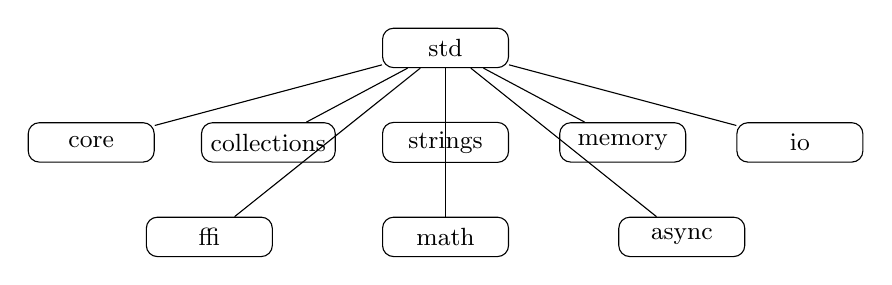
\begin{tikzpicture}[
    box/.style={rectangle, draw, rounded corners, minimum width=1.6cm, minimum height=0.5cm, font=\small}
]
    % Root node
    \node[box] (std) at (0,0) {std};

    % First row of children
    \node[box] (core) at (-4.5,-1.2) {core};
    \node[box] (collections) at (-2.25,-1.2) {collections};
    \node[box] (strings) at (0,-1.2) {strings};
    \node[box] (memory) at (2.25,-1.2) {memory};
    \node[box] (io) at (4.5,-1.2) {io};

    % Second row of children
    \node[box] (ffi) at (-3,-2.4) {ffi};
    \node[box] (math) at (0,-2.4) {math};
    \node[box] (async) at (3,-2.4) {async};

    % Draw connections
    \draw (std) -- (core);
    \draw (std) -- (collections);
    \draw (std) -- (strings);
    \draw (std) -- (memory);
    \draw (std) -- (io);
    \draw (std) -- (ffi);
    \draw (std) -- (math);
    \draw (std) -- (async);
\end{tikzpicture}
\end{center}

\subsection{Module Hierarchy}

\begin{description}
    \item[\texttt{std::core}] Fundamental types: \texttt{Option}, \texttt{Result}, core traits (\texttt{Drop}, \texttt{Clone}, \texttt{From})

    \item[\texttt{std::collections}] Data structures: \texttt{Vec}, \texttt{HashMap}, \texttt{HashSet}, \texttt{VecDeque}, \texttt{BitSet}, \texttt{SlotMap}

    \item[\texttt{std::string}] String handling: \texttt{Str} (borrowed), \texttt{String} (owned), \texttt{StringBuilder}, formatting

    \item[\texttt{std::memory}] Memory management: \texttt{MemoryBlock}, \texttt{Slice}, chip memory pools, allocators

    \item[\texttt{std::io}] Input/output: file operations, console I/O, ANSI terminal support

    \item[\texttt{amiga::raw}] AmigaOS bindings: Exec, DOS, Graphics, Intuition, and 70+ other libraries

    \item[\texttt{std::math}] Mathematics: fixed-point operations, vectors, angles, square roots

    \item[\texttt{std::async}] Asynchronous programming: futures, executors, sleep operations

    \item[\texttt{amiga::sys::hardware}] Hardware access: CPU detection, chipset identification, custom registers

    \item[\texttt{amiga::ui}] User interface: windows, screens, menus, gadgets, events

    \item[\texttt{amiga::sys::graphics}] Graphics operations: drawing, sprites, copper lists, blitter

    \item[\texttt{amiga::audio}] Audio playback: Paula channels, MOD players, sample management

    \item[\texttt{std::net}] Networking: TCP/UDP sockets, DNS, TLS (requires bsdsocket.library)

    \item[\texttt{std::test}] Testing framework: assertions, test attributes, benchmarking

    \item[\texttt{std::error}] Error types: \texttt{DosError}, \texttt{ExecError}, \texttt{NovusError}
\end{description}

\subsection{Physical Layout}

The library lives in the \texttt{std/} directory of the Novus installation:

\begin{lstlisting}[language=bash]
std/
    core.novus              # Core types (Option, Result, traits)
    prelude.novus           # Common re-exports
    collections/
        vec.novus           # Dynamic array
        hashmap.novus       # Hash map
        hashset.novus       # Hash set
        vecdeque.novus      # Double-ended queue
        bitset.novus        # Bit array
        slotmap.novus       # Generational arena
        ...
    strings/
        core.novus          # Str and String types
        format.novus        # Formatting utilities
        display.novus       # Display trait
    memory/
        block.novus         # MemoryBlock type
        slice.novus         # Slice operations
        chip.novus          # Chip memory utilities
        chip_pool.novus     # Chip memory pooling
        ...
    ffi/
        exec.novus          # Exec library
        dos.novus           # DOS library
        graphics.novus      # Graphics library
        intuition.novus     # Intuition library
        amiga_consts.novus  # All AmigaOS constants
        amiga_structs.novus # All AmigaOS structures
        ...
    ...
\end{lstlisting}

% ============================================================================
\section{The Prelude}
\label{sec:stdlib-prelude}
% ============================================================================

The prelude provides commonly-used types that you'll need in almost every program. Import it to get started quickly:

\begin{lstlisting}
from std::prelude import *
\end{lstlisting}

This imports:

\begin{itemize}
    \item \texttt{Option<T>} and \texttt{Result<T, E>} --- for safe error handling
    \item \texttt{Drop}, \texttt{From} --- core traits
    \item \texttt{Str} --- borrowed string type
    \item \texttt{DosError}, \texttt{ExecError}, \texttt{IntuitionError}, \texttt{GraphicsError}, \texttt{NovusError} --- error types
\end{itemize}

\subsection{Selective Imports}

For explicit control, import only what you need:

\begin{lstlisting}
from std::prelude import Option, Result
\end{lstlisting}

Or import directly from the source module:

\begin{lstlisting}
from std::core import Option, Result, Drop
from std::string import Str, String
from std::error::errors import DosError
\end{lstlisting}

\begin{comingfromc}
In C, you might include multiple headers to get the types you need:

\begin{lstlisting}[language=C]
#include <exec/types.h>
#include <dos/dos.h>
#include <string.h>
\end{lstlisting}

In Novus, the prelude gives you essentials in one import. For AmigaOS types, the \texttt{amiga::raw} modules are organized by library, not by NDK header structure.
\end{comingfromc}

% ============================================================================
\section{Import Conventions}
\label{sec:import-conventions}
% ============================================================================

Novus uses a consistent import ordering convention throughout the standard library and in idiomatic user code.

\subsection{Recommended Import Order}

\begin{lstlisting}
// 1. Core types first
from std::core import Option, Result, Drop, Clone

// 2. Collections
from std::collections::vec import Vec
from std::collections::hashmap import HashMap

// 3. Memory management
from std::memory::block import MemoryBlock
from std::memory::slice import Slice

// 4. Strings
from std::string import Str, String
from std::string import format

// 5. Error types
from std::error::errors import DosError, ExecError, NovusError

// 6. AmigaOS structures
from amiga::raw::structs import Window, Screen, RastPort

// 7. AmigaOS constants
from amiga::raw::consts import MEMF_PUBLIC, MEMF_CHIP

// 8. AmigaOS library functions
from amiga::raw::exec import AllocMem, FreeMem, Wait
from amiga::raw::dos import Open, Close, Read, Write
from amiga::raw::intuition import OpenWindow, CloseWindow

// 9. Other stdlib modules
from std::io::file import println
from std::math::vec2 import Vec2
\end{lstlisting}

\subsection{Wildcard Imports}

Use wildcard imports sparingly---they can cause name collisions:

\begin{lstlisting}
// OK: prelude is designed for wildcard import
from std::prelude import *

// OK: constants are namespaced and rarely collide
from amiga::raw::consts import *

// Avoid: too many names, potential collisions
from amiga::raw::exec import *
from amiga::raw::dos import *

// Better: import specific functions
from amiga::raw::exec import AllocMem, FreeMem, Wait
from amiga::raw::dos import Open, Close, Lock, UnLock
\end{lstlisting}

\subsection{Module Aliases}

For frequently-used modules with long paths, create local aliases:

\begin{lstlisting}
// Not yet supported - planned feature
// use amiga::raw::consts as consts
// use std::collections::hashmap as map

// Current workaround: import specific items
from amiga::raw::consts import MEMF_PUBLIC, MEMF_CHIP, MEMF_FAST
from amiga::raw::consts import MODE_OLDFILE, MODE_NEWFILE
\end{lstlisting}

% ============================================================================
\section{Core Types}
\label{sec:stdlib-core-types}
% ============================================================================

The \texttt{std::core} module defines the fundamental types that permeate all Novus code.

\subsection{Option<T>}

Represents a value that may or may not be present:

\begin{lstlisting}
pub enum Option<T> {
    Some(T),
    None,
}
\end{lstlisting}

\textbf{Key methods:}

\begin{center}
\begin{tabular}{lp{8cm}}
\textbf{Method} & \textbf{Description} \\
\hline
\texttt{is\_some()} & Returns \texttt{true} if value is present \\
\texttt{is\_none()} & Returns \texttt{true} if no value \\
\texttt{unwrap()} & Returns value, panics if \texttt{None} \\
\texttt{unwrap\_or(default)} & Returns value or default \\
\texttt{or(other)} & Returns self if \texttt{Some}, otherwise other \\
\texttt{FromPointer(ptr)} & Creates \texttt{Some} if non-null, \texttt{None} if null \\
\end{tabular}
\end{center}

\begin{lstlisting}
from std::core import Option

fn find_user(id: u32) -> Option<User> {
    if id == 0 {
        return Option::None
    }
    // ... lookup user ...
    return Option::Some(user)
}

// Usage
match find_user(42) {
    Option::Some(user) => println(user.name),
    Option::None => println("User not found")
}

// Or with unwrap_or
let user = find_user(42).unwrap_or(default_user)
\end{lstlisting}

\subsection{Result<T, E>}

Represents either success with a value or failure with an error:

\begin{lstlisting}
pub enum Result<T, E> {
    Ok(T),
    Err(E),
}
\end{lstlisting}

\textbf{Key methods:}

\begin{center}
\begin{tabular}{lp{8cm}}
\textbf{Method} & \textbf{Description} \\
\hline
\texttt{is\_ok()} & Returns \texttt{true} if success \\
\texttt{is\_err()} & Returns \texttt{true} if error \\
\texttt{unwrap()} & Returns value, panics if error \\
\texttt{unwrap\_or(default)} & Returns value or default \\
\texttt{ok()} & Converts to \texttt{Option<T>}, discarding error \\
\texttt{err()} & Converts to \texttt{Option<E>}, discarding value \\
\end{tabular}
\end{center}

\begin{lstlisting}
from std::core import Result
from std::error::errors import DosError

fn load_config(path: *u8) -> Result<Config, DosError> {
    let file = open(path, MODE_OLDFILE)?
    defer { close(file) }

    let data = read_all(&file)?
    parse_config(&data)
}

// Usage with ? operator
fn init() -> Result<(), DosError> {
    let config = load_config("app.cfg")?
    // ... use config ...
    Result::Ok(())
}

// Or with match
match load_config("app.cfg") {
    Result::Ok(config) => use_config(&config),
    Result::Err(e) => println(e.message())
}
\end{lstlisting}

\subsection{Core Traits}

\textbf{Drop} --- Automatic cleanup when a value goes out of scope:

\begin{lstlisting}
pub trait Drop {
    fn drop(&var self)
}

// Example: auto-closing file handle
impl Drop for FileHandle {
    fn drop(&var self) {
        if self.fh != null {
            unsafe { Close(self.fh) }
            self.fh = null
        }
    }
}
\end{lstlisting}

\textbf{Clone} --- Explicit value copying:

\begin{lstlisting}
pub trait Clone {
    fn clone(&self) -> Option<Self>
}

// Returns Option because cloning may allocate and fail
let original = Vec::new()
match original.clone() {
    Option::Some(copy) => { /* use copy */ },
    Option::None => { /* allocation failed */ }
}
\end{lstlisting}

\textbf{From} --- Type conversion:

\begin{lstlisting}
pub trait From<T> {
    fn convert(value: T) -> Self
}

// Example: DosError to NovusError
impl From<DosError> for NovusError {
    fn convert(e: DosError) -> NovusError {
        return NovusError::Dos(e)
    }
}

// Used automatically by ? operator
fn example() -> Result<(), NovusError> {
    let file = open("test.txt", MODE_OLDFILE)?  // DosError -> NovusError
    Result::Ok(())
}
\end{lstlisting}

% ============================================================================
\section{Error Types}
\label{sec:stdlib-errors}
% ============================================================================

The standard library provides error types for each AmigaOS subsystem.

\subsection{Error Type Hierarchy}

\begin{center}
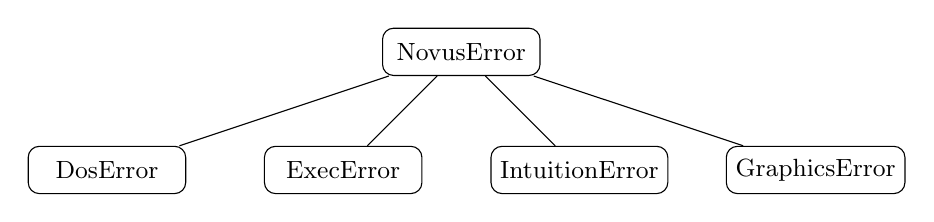
\begin{tikzpicture}[
    level 1/.style={sibling distance=3cm, level distance=1.5cm},
    every node/.style={rectangle, draw, rounded corners, minimum width=2cm, minimum height=0.6cm, font=\small}
]
    \node {NovusError}
        child { node {DosError} }
        child { node {ExecError} }
        child { node {IntuitionError} }
        child { node {GraphicsError} };
\end{tikzpicture}
\end{center}

\subsection{DosError}

Errors from the DOS library (most common variants shown):

\begin{lstlisting}
pub enum DosError {
    NotFound,           // Object not found (IoErr 205)
    AlreadyExists,      // Object already exists (IoErr 203)
    DirNotFound,        // Directory not found (IoErr 204)
    DirectoryNotEmpty,  // Can't delete non-empty dir (IoErr 216)
    PermissionDenied,   // Access denied
    WriteProtected,     // File write protected (IoErr 223)
    DiskFull,           // No space on disk (IoErr 221)
    NoDisk,             // No disk in drive (IoErr 226)
    InvalidLock,        // Bad file lock (IoErr 211)
    NoFreeStore,        // Out of memory (IoErr 103)
    ObjectInUse,        // Object is in use (IoErr 202)
    // ... plus 15+ more variants
    Unknown,            // Unmapped error code
}
\end{lstlisting}

\subsection{ExecError}

Errors from the Exec library:

\begin{lstlisting}
pub enum ExecError {
    NoMem,              // Memory allocation failed
    BadSignal,          // Invalid signal number
    NullReturn,         // Function returned NULL unexpectedly
    BadTask,            // Invalid task pointer
    BadNode,            // Invalid list node
    BadPort,            // Invalid message port
    SignalInUse,        // Signal already allocated
    TaskNotFound,       // FindTask failed
    LibraryNotFound,    // OpenLibrary failed
    InvalidAddress,     // Invalid memory address
    AlignmentError,     // Memory alignment violation
    IndexOutOfBounds,   // Array bounds violation
    CapacityExceeded,   // Fixed buffer full
}
\end{lstlisting}

\subsection{NovusError}

Wrapper for cross-subsystem error handling:

\begin{lstlisting}
pub enum NovusError {
    Dos(DosError),
    Exec(ExecError),
    Intuition(IntuitionError),
    Graphics(GraphicsError),
}

// All error types implement message()
impl DosError {
    pub fn message(&self) -> *u8 {
        match *self {
            DosError::NotFound => "Object not found",
            DosError::DiskFull => "Disk is full",
            // ...
        }
    }
}
\end{lstlisting}

\subsection{Converting Between Error Types}

The \texttt{?} operator automatically converts errors using the \texttt{From} trait:

\begin{lstlisting}
fn load_and_display(path: *u8) -> Result<(), NovusError> {
    // DosError automatically converts to NovusError
    let file = open(path, MODE_OLDFILE)?

    // ExecError also converts
    let buffer = MemoryBlock::alloc(1024, MEMF_PUBLIC)?

    Result::Ok(())
}
\end{lstlisting}

% ============================================================================
\section{Memory Allocation Conventions}
\label{sec:stdlib-memory}
% ============================================================================

The standard library follows consistent patterns for memory allocation.

\subsection{Fallible Allocation}

All allocating functions return \texttt{Option} or \texttt{Result}:

\begin{lstlisting}
// Vec allocation can fail - returns Result with error details
let vec = Vec::with_capacity(1000)?
// Or with explicit match:
match Vec::<i32>::with_capacity(1000) {
    Result::Ok(v) => { /* use v */ },
    Result::Err(e) => { /* out of memory: e.message() */ }
}

// MemoryBlock returns Option (simpler: worked or didn't)
match MemoryBlock::alloc(4096, MEMF_CHIP) {
    Option::Some(block) => { /* use block */ },
    Option::None => { /* allocation failed */ }
}
\end{lstlisting}

\subsection{Memory Type Flags}

AmigaOS memory flags are in \texttt{amiga::raw::amiga\_consts}:

\begin{lstlisting}
from amiga::raw::consts import MEMF_PUBLIC, MEMF_CHIP, MEMF_FAST
from amiga::raw::consts import MEMF_CLEAR, MEMF_LARGEST, MEMF_TOTAL

// Memory flags:
// MEMF_PUBLIC  - Accessible by other tasks
// MEMF_CHIP    - Chip RAM (DMA accessible)
// MEMF_FAST    - Fast RAM (CPU only)
// MEMF_CLEAR   - Zero-fill memory
// MEMF_LARGEST - Return largest available block
// MEMF_TOTAL   - Return total memory of type

// Typical patterns
let chip_buffer = MemoryBlock::alloc(size, MEMF_CHIP | MEMF_CLEAR)?
let fast_buffer = MemoryBlock::alloc(size, MEMF_FAST)?
let any_buffer = MemoryBlock::alloc(size, MEMF_PUBLIC)?
\end{lstlisting}

\subsection{RAII Memory Management}

All stdlib types that allocate implement \texttt{Drop}:

\begin{lstlisting}
fn process_data() -> Result<(), Error> {
    let vec = Vec::with_capacity(100).unwrap()
    let buffer = MemoryBlock::alloc(1024, MEMF_PUBLIC)?

    // ... use vec and buffer ...

    Result::Ok(())
}  // vec and buffer automatically freed here

// Even on early return:
fn early_exit() -> Result<(), Error> {
    let buffer = MemoryBlock::alloc(1024, MEMF_PUBLIC)?

    if some_condition {
        return Result::Err(Error::SomeError)  // buffer freed here
    }

    Result::Ok(())  // buffer freed here too
}
\end{lstlisting}

% ============================================================================
\section{AmigaOS FFI Organization}
\label{sec:stdlib-ffi}
% ============================================================================

The \texttt{amiga::raw} module provides bindings to AmigaOS libraries.

\subsection{Structure}

\begin{lstlisting}[language=bash]
std/amiga/raw/
    amiga_consts.novus    # ALL constants (combined)
    amiga_structs.novus   # ALL structures (combined)
    exec.novus            # Exec library functions
    dos.novus             # DOS library functions
    graphics.novus        # Graphics library functions
    intuition.novus       # Intuition library functions
    gadtools.novus        # GadTools library
    layers.novus          # Layers library
    utility.novus         # Utility library
    ... 70+ more libraries ...
\end{lstlisting}

\subsection{Using FFI Bindings}

\begin{lstlisting}
// Import structures
from amiga::raw::structs import Window, Screen, NewWindow

// Import constants
from amiga::raw::consts import WFLG_CLOSEGADGET, WFLG_DRAGBAR, WFLG_ACTIVATE
from amiga::raw::consts import IDCMP_CLOSEWINDOW, IDCMP_VANILLAKEY

// Import functions
from amiga::raw::intuition import OpenWindow, CloseWindow, WaitPort
from amiga::raw::exec import Wait

// Use in unsafe blocks
unsafe {
    let window = OpenWindow(&new_window_spec)
    if window != null {
        // ... use window ...
        CloseWindow(window)
    }
}
\end{lstlisting}

\subsection{Safe Wrappers}

Many FFI functions have safe wrappers in higher-level modules:

\begin{lstlisting}
// Low-level FFI (requires unsafe)
from amiga::raw::intuition import OpenWindowTags, CloseWindow

// High-level safe wrapper
from amiga::sys::intuition import WindowHandle, WindowBuilder

// Safe usage (no unsafe needed)
let window = WindowBuilder::new()
    .title("My Window")
    .size(320, 200)
    .close_gadget(true)
    .build()?

// Window automatically closed when dropped
\end{lstlisting}

\begin{comingfromc}
In C, you call AmigaOS functions directly and manage lifetimes manually:

\begin{lstlisting}[language=C]
struct Window *win = OpenWindowTags(NULL,
    WA_Title, "My Window",
    WA_Width, 320,
    WA_Height, 200,
    TAG_DONE);
// ... must remember to call CloseWindow(win) ...
\end{lstlisting}

In Novus, the safe wrappers handle cleanup automatically. You can still use the raw FFI when needed, but the wrappers are usually sufficient.
\end{comingfromc}

% ============================================================================
\section{Collections Overview}
\label{sec:stdlib-collections}
% ============================================================================

The \texttt{std::collections} module provides commonly-needed data structures.

\subsection{Available Collections}

\begin{center}
\begin{tabular}{llp{6cm}}
\textbf{Type} & \textbf{Module} & \textbf{Description} \\
\hline
\texttt{Vec<T>} & \texttt{vec} & Dynamic array, contiguous storage \\
\texttt{HashMap<K, V>} & \texttt{hashmap} & Key-value map with O(1) lookup \\
\texttt{HashSet<T>} & \texttt{hashset} & Unique values with O(1) contains \\
\texttt{VecDeque<T>} & \texttt{vecdeque} & Double-ended queue \\
\texttt{BitSet} & \texttt{bitset} & Compact bit array \\
\texttt{SlotMap<T>} & \texttt{slotmap} & Generational arena with stable keys \\
\texttt{RingBuffer<T>} & \texttt{ringbuffer} & Fixed-size circular buffer \\
\texttt{FreeList<T>} & \texttt{freelist} & Object pool with recycling \\
\texttt{SmallVec<T, N>} & \texttt{smallvec} & Stack-allocated up to N elements \\
\texttt{IntrusiveList<T>} & \texttt{intrusive\_list} & Linked list with embedded nodes \\
\end{tabular}
\end{center}

\subsection{Common Patterns}

\begin{lstlisting}
from std::collections::vec import Vec
from std::collections::hashmap import HashMap

// Dynamic array
var scores: Vec<i32> = Vec::new()
scores.push(100)?
scores.push(85)?
scores.push(92)?

for i in 0..scores.len() {
    let score = scores.get(i).unwrap()
    println(f"Score: {score}")
}

// Hash map
var names = HashMap::<u32, *u8>::new()?
names.insert(1, "Alice")?
names.insert(2, "Bob")?

match names.get(1) {
    Option::Some(name) => println(name),
    Option::None => println("Not found")
}
\end{lstlisting}

% ============================================================================
\section{Strings Overview}
\label{sec:stdlib-strings}
% ============================================================================

Novus provides two main string types for different use cases.

\subsection{String Types}

\begin{center}
\begin{tabular}{llp{6cm}}
\textbf{Type} & \textbf{Ownership} & \textbf{Use Case} \\
\hline
\texttt{*u8} & Borrowed & Literal strings, C interop \\
\texttt{Str} & Borrowed & String views with length \\
\texttt{String} & Owned & Mutable, growable strings \\
\texttt{StringBuilder} & Owned & Efficient string building \\
\end{tabular}
\end{center}

\subsection{Usage Examples}

\begin{lstlisting}
from std::string import Str, String, StringBuilder

// Literal (null-terminated, borrowed)
let greeting: *u8 = "Hello, Amiga!"

// Str - borrowed view with known length
let s = Str::from_cstr("Hello").unwrap()
println(f"Length: {s.len()}")

// String - owned, mutable
var name = String::from("Hello")
name.push_str(", World!")
println(name.as_cstr())

// StringBuilder - efficient concatenation
var builder = StringBuilder::new()
builder.push_str("Line 1\n")
builder.push_str("Line 2\n")
builder.push_str("Line 3\n")
let result = builder.to_string()
\end{lstlisting}

% ============================================================================
\section{I/O Overview}
\label{sec:stdlib-io}
% ============================================================================

The \texttt{std::io} module handles input and output operations.

\subsection{Console Output}

\begin{lstlisting}
from std::io::file import print, println

// Basic output
println("Hello, World!")

// With formatting (f-strings)
let name = "Amiga"
let year = 1985
println(f"The {name} was released in {year}")

// Without newline
print("Enter name: ")
\end{lstlisting}

\subsection{File Operations}

\begin{lstlisting}
from amiga::sys::dos import open, close, read, write
from amiga::raw::consts import MODE_OLDFILE, MODE_NEWFILE

// Reading a file
fn read_file(path: *u8) -> Result<Vec<u8>, DosError> {
    let file = open(path, MODE_OLDFILE)?
    defer { close(file) }

    var buffer: Vec<u8> = Vec::with_capacity(4096).unwrap()
    // ... read into buffer ...
    Result::Ok(buffer)
}

// Writing a file
fn write_file(path: *u8, data: &[u8]) -> Result<(), DosError> {
    let file = open(path, MODE_NEWFILE)?
    defer { close(file) }

    write(&file, data)?
    Result::Ok(())
}
\end{lstlisting}

% ============================================================================
\section{Design Principles}
\label{sec:stdlib-principles}
% ============================================================================

The standard library follows several guiding principles.

\subsection{Amiga First}

The library is designed specifically for AmigaOS, not as a portable abstraction layer:

\begin{itemize}
    \item Memory types (chip/fast) are first-class concepts
    \item AmigaOS error codes map directly to error types
    \item Custom chip access is supported, not hidden
    \item RAII works with AmigaOS resource management patterns
\end{itemize}

\subsection{Zero-Cost Abstractions}

High-level types compile to efficient code:

\begin{lstlisting}
// Vec<i32> with bounds checking
let value = vec.get(index)?

// In release mode, compiles to roughly:
//   move.l (a0,d0.l*4),d0
// The Option wrapper is optimized away
\end{lstlisting}

\subsection{Explicit Allocation}

Every allocation is visible and can fail:

\begin{lstlisting}
// Allocations return Option or Result
let vec = Vec::with_capacity(1000)?  // Returns Result<Vec, ExecError>
let map = HashMap::new()?            // Returns Result<HashMap, ExecError>
map.insert(key, value)?              // Allocation happens here
\end{lstlisting}

\subsection{Safe Defaults, Unsafe Escape Hatch}

Most code uses safe wrappers. Raw FFI is available when needed:

\begin{lstlisting}
// Safe (preferred)
let window = Window::open(&spec)?

// Unsafe (when needed)
unsafe {
    let raw_window = OpenWindow(&raw_spec)
}
\end{lstlisting}

% ============================================================================
\section{What's Covered in Part II}
\label{sec:stdlib-roadmap}
% ============================================================================

The following chapters cover each module area in depth:

\begin{description}
    \item[Chapter 13: Core Types] Complete coverage of \texttt{Option}, \texttt{Result}, and core traits

    \item[Chapter 14: Collections] All collection types with performance characteristics and usage patterns

    \item[Chapter 15: Strings] String types, formatting, parsing, and Unicode handling

    \item[Chapter 16: Memory] Memory management, allocators, pools, and chip memory handling

    \item[Chapter 17: I/O] File operations, console I/O, formatting, and buffering

    \item[Chapter 18: Math] Fixed-point arithmetic, vectors, matrices, and trigonometry

    \item[Chapter 19: AmigaOS Bindings] Using the FFI layer, calling conventions, and safe wrappers
\end{description}

% ============================================================================
\section{Quick Reference}
\label{sec:stdlib-quick-ref}
% ============================================================================

\subsection{Common Imports}

\begin{lstlisting}
// Everything you need for most programs
from std::prelude import *
from std::collections::vec import Vec
from std::io::file import println
from amiga::raw::consts import MEMF_PUBLIC, MEMF_CHIP
\end{lstlisting}

\subsection{Error Handling Pattern}

\begin{lstlisting}
fn main() -> i32 {
    match run() {
        Result::Ok(_) => return 0,
        Result::Err(e) => {
            println(e.message())
            return 1
        }
    }
}

fn run() -> Result<(), NovusError> {
    let config = load_config()?
    let window = open_window(&config)?
    main_loop(&window)?
    Result::Ok(())
}
\end{lstlisting}

\subsection{Memory Allocation Pattern}

\begin{lstlisting}
fn process() -> Result<(), ExecError> {
    // Allocation returns Result
    let buffer = MemoryBlock::alloc(4096, MEMF_PUBLIC)?
    defer { /* buffer automatically freed */ }

    // Use buffer...
    do_work(buffer.as_slice())

    Result::Ok(())
}
\end{lstlisting}

% ============================================================================
\section{Summary}
\label{sec:stdlib-summary}
% ============================================================================

The Novus standard library provides:

\begin{itemize}
    \item \textbf{Core types} --- \texttt{Option}, \texttt{Result}, and traits for safe error handling
    \item \textbf{Collections} --- \texttt{Vec}, \texttt{HashMap}, and specialized containers
    \item \textbf{Strings} --- Borrowed and owned strings with formatting
    \item \textbf{Memory} --- Safe allocation with RAII cleanup
    \item \textbf{I/O} --- File and console operations
    \item \textbf{FFI} --- Complete AmigaOS library bindings
    \item \textbf{Math} --- Fixed-point arithmetic and vectors
    \item \textbf{Async} --- Cooperative multitasking via Exec signals
\end{itemize}

The library is designed for the Amiga: every feature respects the platform's constraints while providing modern ergonomics. Use the prelude for quick starts, import specific modules for explicit control.

The following chapters explore each module in depth, with complete API references and practical examples.

% \chapter{Core Types and Traits}
\label{ch:core-types}

The \texttt{std::core} module is the foundation of Novus's type system. It defines the fundamental types and traits that enable safe error handling, resource management, and generic programming. This chapter provides complete documentation for every type and trait in \texttt{std::core}.

% ============================================================================
\section{Option\textless T\textgreater}
\label{sec:option}
% ============================================================================

\texttt{Option<T>} represents a value that may or may not be present. Use it instead of null pointers to make absence explicit and force handling.

\begin{lstlisting}
pub enum Option<T> {
    Some(T),
    None,
}
\end{lstlisting}

\subsection{When to Use Option}

\begin{itemize}
    \item Function might not have a value to return (e.g., \texttt{Vec::pop()})
    \item A field is optional
    \item Lookup operations that may fail to find an element
    \item Simple failure modes where ``not found'' is the only error
\end{itemize}

\begin{notebox}
Use \texttt{Option} when there's only one failure mode. Use \texttt{Result} when you need to distinguish between different error conditions.
\end{notebox}

\subsection{Creating Options}

\begin{lstlisting}
// Explicit construction
let some_value: Option<i32> = Option::Some(42)
let no_value: Option<i32> = Option::None

// From a pointer (non-null check)
let ptr: *u8 = get_some_pointer()
let opt = Option::FromPointer(ptr)  // Some(ptr) if non-null, None otherwise
\end{lstlisting}

\subsection{Option Methods}

\begin{center}
\begin{tabular}{lp{8cm}}
\textbf{Method} & \textbf{Description} \\
\hline
\texttt{is\_some(self) -> bool} & Returns \texttt{true} if the option contains a value \\
\texttt{is\_none(self) -> bool} & Returns \texttt{true} if the option is \texttt{None} \\
\texttt{unwrap(self) -> T} & Returns the value, panics if \texttt{None} \\
\texttt{unwrap\_or(self, default: T) -> T} & Returns the value or a default \\
\texttt{unwrap\_or\_else(self, default: T) -> T} & Same as \texttt{unwrap\_or} (closures planned) \\
\texttt{or(self, optb: Option<T>) -> Option<T>} & Returns self if \texttt{Some}, otherwise \texttt{optb} \\
\texttt{contains(self, val: T) -> bool} & Returns \texttt{true} if contains the value (requires \texttt{Eq}) \\
\texttt{ok\_or<E>(self, err: E) -> Result<T, E>} & Converts to \texttt{Result}, mapping \texttt{None} to \texttt{Err(err)} \\
\texttt{FromPointer(ptr: *T) -> Option<*T>} & Creates \texttt{Some(ptr)} if non-null, \texttt{None} otherwise \\
\end{tabular}
\end{center}

\subsection{Pattern Matching with Option}

The idiomatic way to handle \texttt{Option} is with pattern matching:

\begin{lstlisting}
fn find_user(id: u32) -> Option<User> {
    // ... lookup logic ...
}

// Exhaustive match
match find_user(42) {
    Option::Some(user) => {
        println(user.name)
    },
    Option::None => {
        println("User not found")
    }
}

// If-let for single-arm matches
if let Option::Some(user) = find_user(42) {
    println(user.name)
}

// While-let for iteration
var stack = create_stack()
while let Option::Some(item) = stack.pop() {
    process(item)
}
\end{lstlisting}

\subsection{Combining Options}

\begin{lstlisting}
// Chain with or()
let primary = get_primary_config()
let fallback = get_fallback_config()
let config = primary.or(fallback)  // Use fallback if primary is None

// Convert to Result for richer error info
let user = find_user(id).ok_or(UserError::NotFound)?

// Check contents
let x = Option::Some(42)
if x.contains(42) {
    println("Found 42!")
}
\end{lstlisting}

\begin{warningbox}
\textbf{Avoid \texttt{unwrap()} in library code.} It panics on \texttt{None}, crashing the program. Use \texttt{unwrap\_or()}, pattern matching, or the \texttt{?} operator with \texttt{ok\_or()} instead.
\end{warningbox}

% ============================================================================
\section{Result\textless T, E\textgreater}
\label{sec:result}
% ============================================================================

\texttt{Result<T, E>} represents an operation that can succeed with value \texttt{T} or fail with error \texttt{E}. It's the primary mechanism for error handling in Novus.

\begin{lstlisting}
pub enum Result<T, E> {
    Ok(T),
    Err(E),
}
\end{lstlisting}

\subsection{When to Use Result}

\begin{itemize}
    \item Operations that can fail in multiple ways
    \item I/O operations (file, network, hardware)
    \item Memory allocation
    \item Parsing and validation
    \item Any operation where callers need error details
\end{itemize}

\subsection{Result Methods}

\begin{center}
\begin{tabular}{lp{8cm}}
\textbf{Method} & \textbf{Description} \\
\hline
\texttt{is\_ok(self) -> bool} & Returns \texttt{true} if the result is \texttt{Ok} \\
\texttt{is\_err(self) -> bool} & Returns \texttt{true} if the result is \texttt{Err} \\
\texttt{unwrap(self) -> T} & Returns the value, panics if \texttt{Err} \\
\texttt{unwrap\_err(self) -> E} & Returns the error, panics if \texttt{Ok} \\
\texttt{unwrap\_or(self, default: T) -> T} & Returns the value or a default \\
\texttt{or(self, res: Result<T, E>) -> Result<T, E>} & Returns self if \texttt{Ok}, otherwise \texttt{res} \\
\texttt{ok(self) -> Option<T>} & Converts \texttt{Ok(v)} to \texttt{Some(v)}, \texttt{Err} to \texttt{None} \\
\texttt{err(self) -> Option<E>} & Converts \texttt{Err(e)} to \texttt{Some(e)}, \texttt{Ok} to \texttt{None} \\
\end{tabular}
\end{center}

\subsection{The ? Operator}

The \texttt{?} operator is syntactic sugar for early return on error:

\begin{lstlisting}
fn read_config(path: *u8) -> Result<Config, DosError> {
    let file = open(path, MODE_OLDFILE)?  // Returns Err early if failed
    defer { close(file) }

    let data = read_all(file)?
    let config = parse_config(data)?

    return Result::Ok(config)
}

// Equivalent without ?:
fn read_config_verbose(path: *u8) -> Result<Config, DosError> {
    match open(path, MODE_OLDFILE) {
        Result::Ok(file) => {
            defer { close(file) }
            match read_all(file) {
                Result::Ok(data) => {
                    match parse_config(data) {
                        Result::Ok(config) => return Result::Ok(config),
                        Result::Err(e) => return Result::Err(e)
                    }
                },
                Result::Err(e) => return Result::Err(e)
            }
        },
        Result::Err(e) => return Result::Err(e)
    }
}
\end{lstlisting}

\subsection{Error Type Conversion with ?}

The \texttt{?} operator automatically converts error types using the \texttt{From} trait:

\begin{lstlisting}
// DosError -> NovusError conversion is automatic with ?
fn load_and_display(path: *u8) -> Result<(), NovusError> {
    let data = read_file(path)?         // DosError -> NovusError
    let window = open_window()?         // IntuitionError -> NovusError
    draw_data(window, data)?            // GraphicsError -> NovusError
    return Result::Ok(())
}
\end{lstlisting}

This works because \texttt{impl From<DosError> for NovusError} exists in the error module.

\subsection{Pattern Matching with Result}

\begin{lstlisting}
match allocate_buffer(size) {
    Result::Ok(buffer) => {
        // Use buffer
        process(buffer)
    },
    Result::Err(ExecError::NoMem) => {
        println("Out of memory!")
    },
    Result::Err(e) => {
        // Handle other errors
        println(e.message())
    }
}
\end{lstlisting}

\subsection{Converting Between Option and Result}

\begin{lstlisting}
// Option -> Result: provide an error for None case
let user = find_user(id).ok_or(UserError::NotFound)?

// Result -> Option: discard error information
let maybe_value = risky_operation().ok()
\end{lstlisting}

% ============================================================================
\section{LibraryVersion}
\label{sec:library-version}
% ============================================================================

\texttt{LibraryVersion} represents semantic version information for AmigaOS libraries:

\begin{lstlisting}
pub struct LibraryVersion {
    major: u16,
    minor: u16,
    patch: u16,
}
\end{lstlisting}

\subsection{LibraryVersion Methods}

\begin{lstlisting}
// Creation
let version = LibraryVersion::new(39, 5, 0)

// Access components
let major = version.major()  // 39
let minor = version.minor()  // 5
let patch = version.patch()  // 0

// Comparison (returns: negative if <, zero if ==, positive if >)
let cmp_result = version.cmp(&other_version)
if cmp_result < 0 {
    println("version is older")
}
\end{lstlisting}

% ============================================================================
\section{Resource Management Traits}
\label{sec:resource-traits}
% ============================================================================

These traits enable automatic resource management (RAII) and explicit copying.

\subsection{Drop --- Automatic Cleanup}

The \texttt{Drop} trait enables automatic resource cleanup when values go out of scope:

\begin{lstlisting}
pub trait Drop {
    fn drop(&var self)
}
\end{lstlisting}

\textbf{When drop() is called:}
\begin{itemize}
    \item At the end of a block scope
    \item Before reassignment to a variable
    \item Before early returns
    \item When a variable is shadowed
\end{itemize}

\textbf{When drop() is NOT called:}
\begin{itemize}
    \item If the value was moved to another location
    \item If a field was partially moved (only non-moved fields are dropped)
\end{itemize}

\begin{lstlisting}
impl Drop for MemoryBlock {
    fn drop(&var self) {
        if self.size > 0 {
            unsafe { FreeMem(self.ptr, self.size) }
            self.ptr = (*u8)0
            self.size = 0
        }
    }
}

// Usage - cleanup is automatic
fn example() -> Result<(), ExecError> {
    let mem = MemoryBlock::alloc(1024, MEMF_FAST).unwrap()
    // ... use mem ...
    return Result::Ok(())
}  // mem.drop() called automatically here
\end{lstlisting}

\begin{notebox}
\textbf{Drop order:} Variables are dropped in reverse order of creation. Struct fields are dropped in declaration order. \texttt{defer} blocks run before automatic drop.
\end{notebox}

\subsection{Copy --- Implicit Bitwise Copy}

The \texttt{Copy} trait is a marker trait indicating a type can be copied bitwise:

\begin{lstlisting}
pub trait Copy {}
\end{lstlisting}

Types implementing \texttt{Copy} are implicitly copied when passed by value, rather than moved.

\textbf{When to implement Copy:}
\begin{itemize}
    \item Simple value types (integers, bools, pointers)
    \item Small structs containing only \texttt{Copy} types
    \item Wrapper types around primitives
\end{itemize}

\textbf{When NOT to implement Copy:}
\begin{itemize}
    \item Types that own heap memory (\texttt{Vec}, \texttt{String}, \texttt{Box})
    \item Types with \texttt{Drop} implementations
    \item Types containing non-\texttt{Copy} fields
\end{itemize}

\begin{lstlisting}
struct Point { x: i32, y: i32 }
impl Copy for Point {}

let p1 = Point { x: 10, y: 20 }
let p2 = p1  // Copies p1 instead of moving it
// p1 is still valid here!
\end{lstlisting}

\begin{notebox}
Primitive types (\texttt{i32}, \texttt{u32}, \texttt{bool}, etc.) and pointer types are automatically \texttt{Copy} without requiring explicit \texttt{impl}.
\end{notebox}

\subsection{Clone --- Explicit Deep Copy}

The \texttt{Clone} trait provides explicit deep copying for types where copying may allocate:

\begin{lstlisting}
pub trait Clone {
    fn clone(&self) -> Option<Self>
}
\end{lstlisting}

\textbf{Key difference from Copy:}
\begin{itemize}
    \item \texttt{Copy} is implicit and infallible (bitwise)
    \item \texttt{Clone} is explicit and can fail (returns \texttt{Option})
\end{itemize}

\begin{lstlisting}
impl Clone for Vec<T> {
    fn clone(&self) -> Option<Self> {
        // with_capacity returns Result, convert to Option
        var new_vec = match Vec::with_capacity(self.len()) {
            Result::Ok(v) => v,
            Result::Err(_) => return Option::None
        }
        for i in 0..self.len {
            match new_vec.push(self.get(i).unwrap()) {
                Result::Ok(_) => {},
                Result::Err(_) => return Option::None
            }
        }
        return Option::Some(new_vec)
    }
}

// Usage
let original = Vec::new()
original.push(1).ok()  // Ignore result for simple example
original.push(2)?

match original.clone() {
    Option::Some(copy) => {
        // copy is independent of original
    },
    Option::None => {
        // Allocation failed during clone
    }
}
\end{lstlisting}

% ============================================================================
\section{Type Conversion Traits}
\label{sec:conversion-traits}
% ============================================================================

These traits enable type conversions between different types.

\subsection{From\textless T\textgreater\ --- Infallible Conversion}

The \texttt{From} trait enables automatic type conversions:

\begin{lstlisting}
pub trait From<T> {
    fn convert(value: T) -> Self
}
\end{lstlisting}

\begin{notebox}
The method is named \texttt{convert} instead of \texttt{from} because \texttt{from} is a keyword in Novus (used in import statements).
\end{notebox}

Primary use case: automatic error conversions with the \texttt{?} operator.

\begin{lstlisting}
impl From<DosError> for NovusError {
    fn convert(err: DosError) -> NovusError {
        return NovusError::Dos(err)
    }
}

// Now ? automatically converts DosError to NovusError
fn foo() -> Result<i32, NovusError> {
    let file = open_file("test.txt")?  // DosError -> NovusError
    return Result::Ok(42)
}
\end{lstlisting}

\subsection{Into\textless T\textgreater\ --- Consuming Conversion}

The complement to \texttt{From}:

\begin{lstlisting}
pub trait Into<T> {
    fn into(consuming self) -> T
}
\end{lstlisting}

If you implement \texttt{From<A> for B}, you conceptually get \texttt{Into<B> for A}.

\begin{tipbox}
Prefer implementing \texttt{From} over \texttt{Into}. \texttt{From} is more flexible and provides better type inference.
\end{tipbox}

\subsection{TryFrom and TryInto --- Fallible Conversion}

For conversions that can fail:

\begin{lstlisting}
pub trait TryFrom<T, E> {
    fn try_from(value: T) -> Result<Self, E>
}

pub trait TryInto<T, E> {
    fn try_into(consuming self) -> Result<T, E>
}
\end{lstlisting}

\begin{lstlisting}
// Example: parsing strings to numbers
impl TryFrom<Str, ParseError> for i32 {
    fn try_from(s: Str) -> Result<i32, ParseError> {
        return s.parse_i32()
    }
}

let num = i32::try_from("42")?  // Result<i32, ParseError>
\end{lstlisting}

% ============================================================================
\section{Comparison Traits}
\label{sec:comparison-traits}
% ============================================================================

\subsection{Eq --- Equality}

The \texttt{Eq} trait enables equality comparison with \texttt{==} and \texttt{!=}:

\begin{lstlisting}
pub trait Eq {
    fn eq(&self, other: &Self) -> bool
}
\end{lstlisting}

\textbf{Contract:}
\begin{itemize}
    \item Reflexive: \texttt{a.eq(\&a)} must return \texttt{true}
    \item Symmetric: \texttt{a.eq(\&b)} must equal \texttt{b.eq(\&a)}
    \item Transitive: if \texttt{a.eq(\&b)} and \texttt{b.eq(\&c)}, then \texttt{a.eq(\&c)}
\end{itemize}

\begin{lstlisting}
impl Eq for Point {
    fn eq(&self, other: &Point) -> bool {
        return self.x == other.x && self.y == other.y
    }
}
\end{lstlisting}

\subsection{Ord --- Total Ordering}

The \texttt{Ord} trait provides total ordering:

\begin{lstlisting}
pub trait Ord {
    fn cmp(&self, other: &Self) -> i32
}
\end{lstlisting}

Return value semantics:
\begin{itemize}
    \item Negative: \texttt{self < other}
    \item Zero: \texttt{self == other}
    \item Positive: \texttt{self > other}
\end{itemize}

\begin{lstlisting}
impl Ord for Version {
    fn cmp(&self, other: &Version) -> i32 {
        if self.major != other.major {
            return (i32)self.major - (i32)other.major
        }
        if self.minor != other.minor {
            return (i32)self.minor - (i32)other.minor
        }
        return (i32)self.patch - (i32)other.patch
    }
}
\end{lstlisting}

\subsection{PartialOrd --- Comparison Operators}

For types that support \texttt{<}, \texttt{<=}, \texttt{>}, \texttt{>=}:

\begin{lstlisting}
pub trait PartialOrd {
    fn lt(&self, other: &Self) -> bool
    fn le(&self, other: &Self) -> bool
    fn gt(&self, other: &Self) -> bool
    fn ge(&self, other: &Self) -> bool
}
\end{lstlisting}

% ============================================================================
\section{Hash Trait}
\label{sec:hash-trait}
% ============================================================================

The \texttt{Hash} trait enables types to be used as keys in hash-based collections:

\begin{lstlisting}
pub trait Hash {
    fn hash(&self) -> u32
}
\end{lstlisting}

\textbf{Contract:}
\begin{itemize}
    \item If two values are equal (via \texttt{Eq}), they \textbf{must} produce the same hash
    \item Different values \textit{may} produce the same hash (collision)
    \item Hash should distribute values uniformly across the \texttt{u32} range
\end{itemize}

\begin{lstlisting}
impl Hash for Point {
    fn hash(&self) -> u32 {
        // Combine hashes using XOR and FNV-1a mixing constant
        var h: u32 = self.x.hash()
        h = h ^ (self.y.hash() * 2246822507u32)
        return h
    }
}
\end{lstlisting}

\begin{warningbox}
If you implement both \texttt{Hash} and \texttt{Eq}, maintain the invariant: \texttt{a.eq(\&b)} implies \texttt{a.hash() == b.hash()}.
\end{warningbox}

All primitive types (\texttt{u8}, \texttt{u16}, \texttt{u32}, \texttt{i8}, \texttt{i16}, \texttt{i32}, \texttt{bool}) have built-in \texttt{Hash} implementations using FNV-1a inspired mixing.

% ============================================================================
\section{Operator Traits}
\label{sec:operator-traits}
% ============================================================================

These traits enable operator overloading for custom types.

\subsection{Arithmetic Operators}

\begin{lstlisting}
pub trait Add { fn add(&self, other: &Self) -> Self }
pub trait Sub { fn sub(&self, other: &Self) -> Self }
pub trait Mul { fn mul(&self, other: &Self) -> Self }
pub trait Div { fn div(&self, other: &Self) -> Self }
pub trait Rem { fn rem(&self, other: &Self) -> Self }
pub trait Neg { fn neg(&self) -> Self }
\end{lstlisting}

\begin{lstlisting}
impl Add for Point {
    fn add(&self, other: &Point) -> Point {
        return Point { x: self.x + other.x, y: self.y + other.y }
    }
}

let p1 = Point { x: 10, y: 20 }
let p2 = Point { x: 5, y: 15 }
let p3 = p1 + p2  // Point { x: 15, y: 35 }
\end{lstlisting}

\subsection{Index Operators}

\begin{lstlisting}
pub trait Index<I, T> {
    fn index(&self, idx: I) -> T
}

pub trait IndexMut<I, T> {
    fn index_set(&var self, idx: I, value: T)
}
\end{lstlisting}

\begin{lstlisting}
impl Index<u32, i32> for MyArray {
    fn index(&self, idx: u32) -> i32 {
        return self.data[idx]
    }
}

impl IndexMut<u32, i32> for MyArray {
    fn index_set(&var self, idx: u32, value: i32) {
        self.data[idx] = value
    }
}

let arr = MyArray::new()
let val = arr[0]      // Calls index()
arr[0] = 42           // Calls index_set()
\end{lstlisting}

% ============================================================================
\section{Iterator Traits}
\label{sec:iterator-traits}
% ============================================================================

\subsection{Iterable --- For-In Loop Support}

The \texttt{Iterable} trait enables types to be used in for-in loops:

\begin{lstlisting}
pub trait Iterable<T> {
    fn get(&self, index: u32) -> Option<T>
    fn len(&self) -> u32
}
\end{lstlisting}

\begin{lstlisting}
impl<T> Iterable<T> for Vec<T> {
    fn get(&self, index: u32) -> Option<T> { ... }
    fn len(&self) -> u32 { ... }
}

// For-in loop desugars to index-based iteration
for item in vec {
    process(item)
}
\end{lstlisting}

\subsection{Iterator --- Stateful Iteration}

For more advanced iteration patterns:

\begin{lstlisting}
pub trait Iterator<T> {
    fn next(&var self) -> Option<T>
}
\end{lstlisting}

Unlike \texttt{Iterable}, \texttt{Iterator} is stateful and consumed as it advances:

\begin{lstlisting}
struct RangeIter {
    current: u32,
    end: u32,
}

impl Iterator<u32> for RangeIter {
    fn next(&var self) -> Option<u32> {
        if self.current >= self.end {
            return Option::None
        }
        let val = self.current
        self.current = self.current + 1
        return Option::Some(val)
    }
}

// Usage with while-let
var iter = string.split(",")
while let Option::Some(part) = iter.next() {
    process(part)
}
\end{lstlisting}

\subsection{Collection Building Traits}

\begin{lstlisting}
pub trait Extend<T> {
    fn extend_from_ptr(&var self, source: *T, count: u32) -> bool
}

pub trait FromIterator<T> {
    fn from_slice(ptr: *T, count: u32) -> Option<Self>
}
\end{lstlisting}

% ============================================================================
\section{Numeric Traits}
\label{sec:numeric-traits}
% ============================================================================

\subsection{Default --- Default Values}

\begin{lstlisting}
pub trait Default {
    fn default() -> Self
}
\end{lstlisting}

Built-in defaults:
\begin{itemize}
    \item Integers: \texttt{0}
    \item \texttt{bool}: \texttt{false}
    \item \texttt{Option<T>}: \texttt{None}
\end{itemize}

\begin{lstlisting}
impl Default for MyConfig {
    fn default() -> MyConfig {
        return MyConfig { timeout: 1000, retries: 3 }
    }
}

let config = MyConfig::default()
\end{lstlisting}

\subsection{Zero and One --- Identity Elements}

\begin{lstlisting}
pub trait Zero {
    fn zero() -> Self
    fn is_zero(&self) -> bool
}

pub trait One {
    fn one() -> Self
}
\end{lstlisting}

Used in generic numeric algorithms:

\begin{lstlisting}
fn sum<T: Zero + Add>(values: &Vec<T>) -> T {
    var total = T::zero()
    for v in values {
        total = total.add(&v)
    }
    return total
}
\end{lstlisting}

\subsection{Bounded --- Min/Max Values}

\begin{lstlisting}
pub trait Bounded {
    fn min_value() -> Self
    fn max_value() -> Self
}
\end{lstlisting}

\begin{center}
\begin{tabular}{lrr}
\textbf{Type} & \textbf{min\_value()} & \textbf{max\_value()} \\
\hline
\texttt{u8} & 0 & 255 \\
\texttt{u16} & 0 & 65,535 \\
\texttt{u32} & 0 & 4,294,967,295 \\
\texttt{i8} & -128 & 127 \\
\texttt{i16} & -32,768 & 32,767 \\
\texttt{i32} & -2,147,483,648 & 2,147,483,647 \\
\end{tabular}
\end{center}

\subsection{Primitive Trait Implementations Summary}

The following table shows which traits are implemented for primitive types:

\begin{center}
\begin{tabular}{lccccccc}
\textbf{Type} & \textbf{Hash} & \textbf{Eq} & \textbf{Ord} & \textbf{Default} & \textbf{Zero} & \textbf{One} & \textbf{Bounded} \\
\hline
\texttt{u8}, \texttt{u16}, \texttt{u32} & \textbullet & \textbullet & \textbullet & \textbullet & \textbullet & \textbullet & \textbullet \\
\texttt{i8}, \texttt{i16}, \texttt{i32} & \textbullet & \textbullet & \textbullet & \textbullet & \textbullet & \textbullet & \textbullet \\
\texttt{bool} & \textbullet & \textbullet & \textbullet & \textbullet & --- & --- & --- \\
\texttt{Option<T>} & --- & --- & --- & \textbullet & --- & --- & --- \\
\texttt{LibraryVersion} & --- & --- & \textbullet & --- & --- & --- & --- \\
\end{tabular}
\end{center}

All primitive integer and boolean types have complete trait coverage. The \texttt{Copy} trait is implicit for all primitives and pointer types.

% ============================================================================
\section{View Conversion Traits}
\label{sec:view-traits}
% ============================================================================

\subsection{AsRef and AsMut}

Zero-cost reference-to-reference conversions:

\begin{lstlisting}
pub trait AsRef<T> {
    fn as_ref(&self) -> T
}

pub trait AsMut<T> {
    fn as_mut(&var self) -> T
}
\end{lstlisting}

\begin{lstlisting}
// String can be viewed as Str
impl AsRef<Str> for String {
    fn as_ref(&self) -> Str {
        return self.as_str()
    }
}

// Generic function accepting any string-like type
fn process<S: AsRef<Str>>(s: &S) {
    let str_view: Str = s.as_ref()
    // Works with String, PathString, etc.
}
\end{lstlisting}

\subsection{Write --- Unified Output}

\begin{lstlisting}
pub trait Write {
    fn write_bytes(&var self, ptr: *u8, len: u32) -> bool
    fn write_byte(&var self, b: u8) -> bool
}
\end{lstlisting}

Implemented by \texttt{StringBuilder}, \texttt{String}, formatters, and (future) file handles.

% ============================================================================
\section{Error Trait}
\label{sec:error-trait}
% ============================================================================

\begin{lstlisting}
pub trait Error {
    fn message(&self) -> *u8
}
\end{lstlisting}

All stdlib error types implement this trait:

\begin{lstlisting}
impl Error for DosError {
    fn message(&self) -> *u8 {
        match *self {
            DosError::NotFound => return "File not found",
            DosError::DiskFull => return "Disk full",
            _ => return "Unknown error"
        }
    }
}

// Usage
fn handle_error(err: &dyn Error) {
    println(err.message())
}
\end{lstlisting}

% ============================================================================
\section{Function Traits}
\label{sec:function-traits}
% ============================================================================

These traits represent callable types (for future closure support):

\begin{lstlisting}
pub trait FnOnce<Args, Output> {
    fn call_once(consuming self, args: Args) -> Output
}

pub trait FnMut<Args, Output> {
    fn call_mut(&var self, args: Args) -> Output
}

pub trait Fn<Args, Output> {
    fn call(&self, args: Args) -> Output
}
\end{lstlisting}

Hierarchy:
\begin{itemize}
    \item \texttt{Fn} --- can be called repeatedly without mutation
    \item \texttt{FnMut} --- can be called repeatedly with mutation
    \item \texttt{FnOnce} --- can be called at least once (consumes self)
\end{itemize}

\begin{notebox}
Closures are not yet implemented in Novus. These traits are defined for future compatibility.
\end{notebox}

% ============================================================================
\section{Summary}
\label{sec:core-summary}
% ============================================================================

The \texttt{std::core} module provides:

\begin{description}
    \item[Fundamental Types] \texttt{Option<T>}, \texttt{Result<T, E>}, \texttt{LibraryVersion}

    \item[Resource Management] \texttt{Drop} (automatic cleanup), \texttt{Copy} (bitwise copy), \texttt{Clone} (explicit deep copy)

    \item[Type Conversion] \texttt{From}/\texttt{Into} (infallible), \texttt{TryFrom}/\texttt{TryInto} (fallible)

    \item[Comparison] \texttt{Eq} (equality), \texttt{Ord} (total ordering), \texttt{PartialOrd} (operators), \texttt{Hash}

    \item[Operators] \texttt{Add}, \texttt{Sub}, \texttt{Mul}, \texttt{Div}, \texttt{Rem}, \texttt{Neg}, \texttt{Index}, \texttt{IndexMut}

    \item[Iteration] \texttt{Iterable} (for-in), \texttt{Iterator} (stateful), \texttt{Extend}, \texttt{FromIterator}

    \item[Numeric] \texttt{Default}, \texttt{Zero}, \texttt{One}, \texttt{Bounded}

    \item[Views] \texttt{AsRef}, \texttt{AsMut}, \texttt{Write}

    \item[Error Handling] \texttt{Error}

    \item[Functions] \texttt{Fn}, \texttt{FnMut}, \texttt{FnOnce} (future)
\end{description}

\begin{tipbox}
Import commonly used types from the prelude:
\begin{lstlisting}
from std::prelude import *
// Imports: Option, Result, Drop, From, Str, and error types
\end{lstlisting}
\end{tipbox}

% \chapter{Collections}
\label{chap:collections}

The \texttt{std::collections} module provides a comprehensive set of data structures optimized for Amiga systems. Each collection is designed with the constraints and opportunities of 68k processors in mind: deterministic memory management, cache-friendly layouts, and zero hidden allocations.

\section{Overview}

Novus collections fall into several categories based on their use cases:

\begin{table}[h]
\centering
\begin{tabular}{lll}
\textbf{Category} & \textbf{Collections} & \textbf{Use Case} \\
\hline
Sequential & \texttt{Vec}, \texttt{VecDeque}, \texttt{SmallVec} & Ordered elements \\
Associative & \texttt{HashMap}, \texttt{HashSet} & Key-value lookup \\
Bit-level & \texttt{BitSet} & Compact boolean storage \\
Streaming & \texttt{RingBuffer}, \texttt{RingBufferPow2} & Fixed-size queues \\
Intrusive & \texttt{IntrusiveList}, \texttt{PriorityList} & AmigaOS interop \\
Arena & \texttt{SlotMap}, \texttt{ObjectPool} & Stable handles \\
\end{tabular}
\caption{Collection categories and their primary use cases}
\end{table}

\subsection{Choosing the Right Collection}

\begin{itemize}
    \item \textbf{Need a growable array?} Use \texttt{Vec<T>}
    \item \textbf{Need a queue or deque?} Use \texttt{VecDeque<T>}
    \item \textbf{Know the typical size?} Use \texttt{SmallVec<T, N>}
    \item \textbf{Need key-value storage?} Use \texttt{HashMap<K, V>}
    \item \textbf{Need unique values?} Use \texttt{HashSet<T>}
    \item \textbf{Need compact flags?} Use \texttt{BitSet}
    \item \textbf{Need a fixed-size buffer?} Use \texttt{RingBuffer<T>}
    \item \textbf{Interfacing with AmigaOS lists?} Use \texttt{IntrusiveList<T>}
    \item \textbf{Need stable handles to objects?} Use \texttt{SlotMap<T>}
    \item \textbf{Need a pool allocator?} Use \texttt{ObjectPool<T>}
\end{itemize}

%%%%%%%%%%%%%%%%%%%%%%%%%%%%%%%%%%%%%%%%%%%%%%%%%%%%%%%%%%%%%%%%%%%%%%%%%%%%%%%
\section{Vec<T> --- Dynamic Array}
\label{sec:vec}
%%%%%%%%%%%%%%%%%%%%%%%%%%%%%%%%%%%%%%%%%%%%%%%%%%%%%%%%%%%%%%%%%%%%%%%%%%%%%%%

\texttt{Vec<T>} is a contiguous, growable array type with heap-allocated contents. It's the most commonly used collection in Novus, similar to Rust's \texttt{Vec} or C++'s \texttt{std::vector}.

\begin{lstlisting}
from std::collections::vec import Vec

fn example() -> Result<(), ExecError> {
    // Create an empty vector
    var numbers = Vec::<u32>::new()

    // Push elements (may allocate)
    numbers.push(1)?
    numbers.push(2)?
    numbers.push(3)?

    // Access by index
    match numbers.get(0) {
        Option::Some(val) => print_u32(val),
        Option::None => {}
    }

    // Pop from the end
    match numbers.pop() {
        Option::Some(val) => print_u32(val),  // 3
        Option::None => {}
    }

    return Result::Ok(())
}
// Memory automatically freed when numbers goes out of scope
\end{lstlisting}

\subsection{Creating Vectors}

\begin{lstlisting}
// Empty vector (zero capacity, no allocation)
var v1 = Vec::<u32>::new()

// Pre-allocated capacity (reduces reallocations)
var v2 = Vec::<u32>::with_capacity(100)?
\end{lstlisting}

\begin{notebox}
\texttt{Vec::new()} performs no allocation. Memory is only allocated on the first \texttt{push()} or \texttt{reserve()} call.
\end{notebox}

\subsection{Core Operations}

\begin{table}[h]
\centering
\begin{tabular}{llll}
\textbf{Method} & \textbf{Returns} & \textbf{Complexity} & \textbf{Description} \\
\hline
\texttt{push(val)} & \texttt{Result<(), ExecError>} & O(1)* & Append to end \\
\texttt{pop()} & \texttt{Option<T>} & O(1) & Remove from end \\
\texttt{get(idx)} & \texttt{Option<T>} & O(1) & Read element \\
\texttt{set(idx, val)} & \texttt{Result<(), ExecError>} & O(1) & Write element \\
\texttt{insert(idx, val)} & \texttt{Result<(), ExecError>} & O(n) & Insert at position \\
\texttt{remove(idx)} & \texttt{Result<T, ExecError>} & O(n) & Remove at position \\
\texttt{len()} & \texttt{u32} & O(1) & Element count \\
\texttt{capacity()} & \texttt{u32} & O(1) & Current capacity \\
\texttt{is\_empty()} & \texttt{bool} & O(1) & Check if empty \\
\texttt{clear()} & \texttt{()} & O(1) & Remove all elements \\
\texttt{reserve(n)} & \texttt{Result<(), ExecError>} & O(n) & Ensure capacity \\
\texttt{shrink\_to\_fit()} & \texttt{Result<(), ExecError>} & O(n) & Reduce capacity \\
\end{tabular}
\caption{\texttt{Vec<T>} method summary. *Amortized O(1), O(n) when growing.}
\end{table}

\subsection{Growth Strategy}

When a \texttt{Vec} needs more capacity, it doubles its current capacity (minimum 4 elements). This amortized doubling strategy provides O(1) push operations on average while minimizing reallocations.

\begin{lstlisting}
var v = Vec::<u32>::new()
// capacity: 0

v.push(1)?   // allocates 4 elements
// capacity: 4

v.push(2)?
v.push(3)?
v.push(4)?
v.push(5)?   // reallocates to 8 elements
// capacity: 8
\end{lstlisting}

\begin{comingfromc}
Unlike C's \texttt{realloc()}, Novus always allocates new memory and copies data. This is because AmigaOS's \texttt{AllocMem}/\texttt{FreeMem} don't support in-place growth. Pre-allocate with \texttt{with\_capacity()} when you know the expected size.
\end{comingfromc}

\subsection{Iteration}

\texttt{Vec<T>} implements the \texttt{Iterable<T>} trait, enabling use in \texttt{for-in} loops:

\begin{lstlisting}
var numbers = Vec::<u32>::new()
numbers.push(10)?
numbers.push(20)?
numbers.push(30)?

for num in numbers {
    print_u32(num)
}
// Prints: 10 20 30
\end{lstlisting}

\subsection{Memory and RAII}

\texttt{Vec<T>} implements \texttt{Drop}, automatically freeing its memory when it goes out of scope:

\begin{lstlisting}
fn process_data() -> Result<(), ExecError> {
    var data = Vec::<u32>::with_capacity(1000)?

    // ... use data ...

    return Result::Ok(())
}  // data.drop() called automatically, memory freed
\end{lstlisting}

%%%%%%%%%%%%%%%%%%%%%%%%%%%%%%%%%%%%%%%%%%%%%%%%%%%%%%%%%%%%%%%%%%%%%%%%%%%%%%%
\section{VecDeque<T> --- Double-Ended Queue}
\label{sec:vecdeque}
%%%%%%%%%%%%%%%%%%%%%%%%%%%%%%%%%%%%%%%%%%%%%%%%%%%%%%%%%%%%%%%%%%%%%%%%%%%%%%%

\texttt{VecDeque<T>} is a double-ended queue implemented as a ring buffer. It provides O(1) insertion and removal at both ends, making it ideal for queues, sliding windows, and work-stealing algorithms.

\begin{lstlisting}
from std::collections::vecdeque import VecDeque

fn message_queue() -> Result<(), ExecError> {
    var queue = VecDeque::<Message>::with_capacity(32)?

    // Enqueue (add to back)
    queue.push_back(msg1)?
    queue.push_back(msg2)?

    // Urgent message to front
    queue.push_front(urgent_msg)?

    // Dequeue (remove from front)
    match queue.pop_front() {
        Option::Some(msg) => process(msg),
        Option::None => {}  // empty
    }

    return Result::Ok(())
}
\end{lstlisting}

\subsection{Ring Buffer Implementation}

Internally, \texttt{VecDeque} uses a circular buffer with \texttt{head} and \texttt{len} indices:

\begin{lstlisting}
// Logical view:    [A, B, C, D]
// Physical memory: [C, D, _, _, A, B]  (head=4, len=4)
//                           ^-- unused space
\end{lstlisting}

This allows both \texttt{push\_front} and \texttt{push\_back} to be O(1) operations without shifting elements.

\subsection{Core Operations}

\begin{table}[h]
\centering
\begin{tabular}{lll}
\textbf{Method} & \textbf{Returns} & \textbf{Description} \\
\hline
\texttt{push\_back(val)} & \texttt{Result<(), ExecError>} & Add to back (enqueue) \\
\texttt{push\_front(val)} & \texttt{Result<(), ExecError>} & Add to front \\
\texttt{pop\_back()} & \texttt{Option<T>} & Remove from back \\
\texttt{pop\_front()} & \texttt{Option<T>} & Remove from front (dequeue) \\
\texttt{front()} & \texttt{Option<T>} & Peek at front \\
\texttt{back()} & \texttt{Option<T>} & Peek at back \\
\texttt{get(idx)} & \texttt{Option<T>} & Access by logical index \\
\texttt{rotate\_left(n)} & \texttt{()} & Rotate elements left \\
\texttt{rotate\_right(n)} & \texttt{()} & Rotate elements right \\
\end{tabular}
\caption{\texttt{VecDeque<T>} method summary}
\end{table}

\subsection{Use Cases}

\begin{itemize}
    \item \textbf{FIFO queues}: \texttt{push\_back()} + \texttt{pop\_front()}
    \item \textbf{LIFO stacks}: \texttt{push\_back()} + \texttt{pop\_back()}
    \item \textbf{Sliding windows}: Maintain a fixed-size window of recent values
    \item \textbf{Priority bypass}: Insert urgent items at front
\end{itemize}

%%%%%%%%%%%%%%%%%%%%%%%%%%%%%%%%%%%%%%%%%%%%%%%%%%%%%%%%%%%%%%%%%%%%%%%%%%%%%%%
\section{SmallVec<T, N> --- Small Vector Optimization}
\label{sec:smallvec}
%%%%%%%%%%%%%%%%%%%%%%%%%%%%%%%%%%%%%%%%%%%%%%%%%%%%%%%%%%%%%%%%%%%%%%%%%%%%%%%

\texttt{SmallVec<T, N>} is a vector that uses the const generic \texttt{N} as its initial capacity. This reduces allocation overhead when you know a typical size.

\begin{lstlisting}
from std::collections::smallvec import SmallVec

// Create a SmallVec with initial capacity of 8
var coords = SmallVec::<Point, 8>::new()

// First push allocates N=8 capacity
coords.push(Point { x: 10, y: 20 })?

// Subsequent pushes use existing capacity
coords.push(Point { x: 30, y: 40 })?
\end{lstlisting}

\begin{notebox}
The current implementation allocates \texttt{N} elements on first push. A future version may store small arrays inline (true small-vector optimization) once Novus supports array types with const generic sizes.
\end{notebox}

\subsection{When to Use SmallVec}

Use \texttt{SmallVec} when:
\begin{itemize}
    \item You know the typical size of your collection
    \item Most instances stay below a certain threshold
    \item You want to avoid the overhead of dynamic resizing
\end{itemize}

\begin{lstlisting}
// A polygon usually has 3-8 vertices
var vertices = SmallVec::<Vertex, 8>::new()

// A function usually has 0-4 parameters
var params = SmallVec::<Param, 4>::new()
\end{lstlisting}

\subsection{Core Operations}

\texttt{SmallVec} provides the same interface as \texttt{Vec}:

\begin{table}[h]
\centering
\begin{tabular}{lll}
\textbf{Method} & \textbf{Returns} & \textbf{Description} \\
\hline
\texttt{push(val)} & \texttt{Result<(), ExecError>} & Append element \\
\texttt{pop()} & \texttt{Option<T>} & Remove last element \\
\texttt{get(idx)} & \texttt{Option<T>} & Read element by index \\
\texttt{get\_mut(idx)} & \texttt{Option<*T>} & Get mutable pointer \\
\texttt{len()} & \texttt{u32} & Element count \\
\texttt{capacity()} & \texttt{u32} & Current capacity \\
\texttt{is\_empty()} & \texttt{bool} & Check if empty \\
\texttt{clear()} & \texttt{()} & Remove all elements \\
\end{tabular}
\caption{\texttt{SmallVec<T, N>} method summary}
\end{table}

%%%%%%%%%%%%%%%%%%%%%%%%%%%%%%%%%%%%%%%%%%%%%%%%%%%%%%%%%%%%%%%%%%%%%%%%%%%%%%%
\section{HashMap<K, V> --- Hash Map}
\label{sec:hashmap}
%%%%%%%%%%%%%%%%%%%%%%%%%%%%%%%%%%%%%%%%%%%%%%%%%%%%%%%%%%%%%%%%%%%%%%%%%%%%%%%

\texttt{HashMap<K, V>} is a hash table with generic keys using open addressing and linear probing. Keys must implement the \texttt{Hash} and \texttt{Eq} traits.

\begin{lstlisting}
from std::collections::hashmap import HashMap

fn symbol_table() -> Result<(), ExecError> {
    var symbols: HashMap<u32, u32> = HashMap::new()?

    // Insert key-value pairs
    symbols.insert(hash("foo"), 100)?
    symbols.insert(hash("bar"), 200)?

    // Lookup by key
    match symbols.get(&hash("foo")) {
        Option::Some(val_ptr) => print_u32(*val_ptr),
        Option::None => print("not found")
    }

    // Check existence
    if symbols.contains_key(&hash("foo")) {
        // key exists
    }

    // Remove
    match symbols.remove(&hash("bar")) {
        Option::Some(old_val) => {},  // was 200
        Option::None => {}
    }

    return Result::Ok(())
}
\end{lstlisting}

\subsection{Implementation Details}

\texttt{HashMap} uses several optimizations for 68k performance:

\begin{itemize}
    \item \textbf{Open addressing}: All entries in a single array (better cache locality)
    \item \textbf{Linear probing}: Simple collision resolution
    \item \textbf{Tombstones}: Lazy deletion for correct probe sequences
    \item \textbf{Power-of-2 capacity}: Fast modulo via bitwise AND
    \item \textbf{70\% load factor}: Automatic resize threshold
    \item \textbf{Cached entry size}: Avoids expensive multiplication
\end{itemize}

\subsection{Core Operations}

\begin{table}[h]
\centering
\begin{tabular}{lll}
\textbf{Method} & \textbf{Returns} & \textbf{Description} \\
\hline
\texttt{insert(k, v)} & \texttt{Result<Option<V>, ExecError>} & Insert/update \\
\texttt{get(\&k)} & \texttt{Option<\&V>} & Lookup by key \\
\texttt{get\_mut(\&k)} & \texttt{Option<\&var V>} & Mutable lookup \\
\texttt{remove(\&k)} & \texttt{Option<V>} & Remove by key \\
\texttt{contains\_key(\&k)} & \texttt{bool} & Check existence \\
\texttt{len()} & \texttt{u32} & Number of pairs \\
\texttt{is\_empty()} & \texttt{bool} & Check if empty \\
\texttt{clear()} & \texttt{()} & Remove all entries \\
\texttt{reserve(n)} & \texttt{Result<(), ExecError>} & Reserve capacity \\
\texttt{compact()} & \texttt{Result<(), ExecError>} & Clear tombstones \\
\texttt{iter()} & \texttt{HashMapIter<K, V>} & Iterator \\
\end{tabular}
\caption{\texttt{HashMap<K, V>} method summary}
\end{table}

\subsection{Iteration}

The iterator returns \texttt{KeyValueRef} structs containing \emph{pointers} to the keys and values:

\begin{lstlisting}
// KeyValueRef structure (returned by iter().next())
struct KeyValueRef<K, V> {
    key: *K,     // Pointer to key
    value: *V,   // Pointer to value
}
\end{lstlisting}

Use pointer dereferencing (\texttt{*}) to access the actual values:

\begin{lstlisting}
var map: HashMap<u32, u32> = HashMap::new()?
map.insert(1, 100)?
map.insert(2, 200)?

var iter = map.iter()
while true {
    match iter.next() {
        Option::Some(kv) => {
            // Note: kv.key and kv.value are pointers
            print_u32(*kv.key)    // Dereference to get key
            print_u32(*kv.value)  // Dereference to get value
        },
        Option::None => break
    }
}
\end{lstlisting}

\begin{warningbox}
Do not modify the map while iterating. This invalidates the iterator and may cause undefined behavior.
\end{warningbox}

\subsection{Key Requirements}

Keys must implement \texttt{Hash} and \texttt{Eq}:

\begin{lstlisting}
struct Point {
    x: i32,
    y: i32,
}

impl Hash for Point {
    fn hash(&self) -> u32 {
        var h: u32 = self.x.hash()
        h = h ^ (self.y.hash() * 2246822507)
        return h
    }
}

impl Eq for Point {
    fn eq(&self, other: &Point) -> bool {
        return self.x == other.x && self.y == other.y
    }
}

// Now Point can be used as a HashMap key
var point_map: HashMap<Point, u32> = HashMap::new()?
\end{lstlisting}

%%%%%%%%%%%%%%%%%%%%%%%%%%%%%%%%%%%%%%%%%%%%%%%%%%%%%%%%%%%%%%%%%%%%%%%%%%%%%%%
\section{HashSet<T> --- Hash Set}
\label{sec:hashset}
%%%%%%%%%%%%%%%%%%%%%%%%%%%%%%%%%%%%%%%%%%%%%%%%%%%%%%%%%%%%%%%%%%%%%%%%%%%%%%%

\texttt{HashSet<T>} is a set of unique values backed by \texttt{HashMap<T, ()>}. It provides O(1) insert, remove, and contains operations.

\begin{lstlisting}
from std::collections::hashset import HashSet

fn unique_ids() -> Result<(), ExecError> {
    var seen: HashSet<u32> = HashSet::new()?

    // Insert returns Ok(true) for new, Ok(false) for existing
    seen.insert(1)?  // Ok(true)
    seen.insert(2)?  // Ok(true)
    seen.insert(1)?  // Ok(false) - already present

    // Check membership
    if seen.contains(&1) {
        // value is in set
    }

    // Remove
    seen.remove(&2)  // returns true

    return Result::Ok(())
}
\end{lstlisting}

\subsection{Set Operations}

\begin{lstlisting}
var a: HashSet<u32> = HashSet::new()?
var b: HashSet<u32> = HashSet::new()?

// Check subset relationship
if a.is_subset(&b) {
    // every element in a is also in b
}

// Check if sets have common elements
if a.intersects(&b) {
    // at least one element in common
}
\end{lstlisting}

%%%%%%%%%%%%%%%%%%%%%%%%%%%%%%%%%%%%%%%%%%%%%%%%%%%%%%%%%%%%%%%%%%%%%%%%%%%%%%%
\section{BitSet --- Compact Bit Storage}
\label{sec:bitset}
%%%%%%%%%%%%%%%%%%%%%%%%%%%%%%%%%%%%%%%%%%%%%%%%%%%%%%%%%%%%%%%%%%%%%%%%%%%%%%%

\texttt{BitSet} provides compact storage for boolean flags using 1 bit per element. This is 32x more memory-efficient than a \texttt{bool} array, essential for resource-constrained Amiga development.

\begin{lstlisting}
from std::collections::bitset import BitSet

fn track_sprites() -> Result<(), ExecError> {
    // 64 bits = 8 bytes (vs 64 bytes for bool array)
    match BitSet::with_capacity(64) {
        Option::Some(var active_sprites) => {
            // Set bits
            active_sprites.set(0)   // sprite 0 is active
            active_sprites.set(5)   // sprite 5 is active

            // Check bits
            if active_sprites.get(0) {
                // sprite 0 is active
            }

            // Count active sprites
            let count = active_sprites.count_ones()  // 2

            // Find first active sprite
            match active_sprites.find_first_set() {
                Option::Some(idx) => {},  // idx == 0
                Option::None => {}
            }
        },
        Option::None => {}
    }

    return Result::Ok(())
}
\end{lstlisting}

\subsection{Bitwise Operations}

\begin{lstlisting}
var a = BitSet::with_capacity(32)?
var b = BitSet::with_capacity(32)?

// Set some bits
a.set(0)
a.set(2)
b.set(1)
b.set(2)

// Bitwise operations (mutate a)
a.and(&b)   // a = a & b (intersection)
a.or(&b)    // a = a | b (union)
a.xor(&b)   // a = a ^ b (symmetric difference)
a.not()     // a = ~a (complement)
\end{lstlisting}

\subsection{Core Operations}

\begin{table}[h]
\centering
\begin{tabular}{lll}
\textbf{Method} & \textbf{Returns} & \textbf{Description} \\
\hline
\texttt{set(idx)} & \texttt{bool} & Set bit to true \\
\texttt{clear(idx)} & \texttt{bool} & Set bit to false \\
\texttt{get(idx)} & \texttt{bool} & Get bit value \\
\texttt{toggle(idx)} & \texttt{bool} & Flip bit \\
\texttt{set\_all()} & \texttt{()} & Set all bits \\
\texttt{clear\_all()} & \texttt{()} & Clear all bits \\
\texttt{count\_ones()} & \texttt{u32} & Population count \\
\texttt{count\_zeros()} & \texttt{u32} & Count cleared bits \\
\texttt{find\_first\_set()} & \texttt{Option<u32>} & First set bit \\
\texttt{find\_first\_clear()} & \texttt{Option<u32>} & First clear bit \\
\texttt{all()} & \texttt{bool} & All bits set? \\
\texttt{any()} & \texttt{bool} & Any bit set? \\
\texttt{none()} & \texttt{bool} & No bits set? \\
\end{tabular}
\caption{\texttt{BitSet} method summary}
\end{table}

\begin{comingfromc}
\texttt{BitSet} uses Brian Kernighan's algorithm for population count and binary search for first-set-bit. On 68020+, these could be replaced with native \texttt{BFFFO} (find first one) instructions for better performance.
\end{comingfromc}

%%%%%%%%%%%%%%%%%%%%%%%%%%%%%%%%%%%%%%%%%%%%%%%%%%%%%%%%%%%%%%%%%%%%%%%%%%%%%%%
\section{RingBuffer<T> --- Fixed-Size Circular Buffer}
\label{sec:ringbuffer}
%%%%%%%%%%%%%%%%%%%%%%%%%%%%%%%%%%%%%%%%%%%%%%%%%%%%%%%%%%%%%%%%%%%%%%%%%%%%%%%

\texttt{RingBuffer<T>} is a fixed-capacity circular buffer ideal for streaming data, audio buffering, and interrupt-safe producer-consumer patterns.

\begin{lstlisting}
from std::collections::ringbuffer import RingBuffer, RingBufferPow2

fn audio_buffer() {
    // Create a 256-sample buffer
    match RingBuffer::<i16>::with_capacity(256) {
        Option::Some(var buffer) => {
            // Producer (e.g., interrupt handler)
            buffer.push_back(sample)  // returns false if full

            // Consumer (e.g., main task)
            match buffer.pop_front() {
                Option::Some(sample) => play(sample),
                Option::None => {}  // buffer empty
            }
        },
        Option::None => {}
    }
}
\end{lstlisting}

\subsection{Power-of-2 Optimization}

For maximum performance, use \texttt{RingBufferPow2<T>} which uses bitwise AND instead of modulo for index wrapping:

\begin{lstlisting}
// Request 100, get 128 (next power of 2)
match RingBufferPow2::<Sample>::with_capacity(100) {
    Option::Some(var buffer) => {
        // buffer.capacity() == 128
        // ~6x faster push/pop on 68000
    },
    Option::None => {}
}
\end{lstlisting}

\begin{tipbox}
\textbf{Performance on 68000}:
\begin{itemize}
    \item \texttt{RingBuffer::push\_back}: $\sim$150 cycles (uses modulo)
    \item \texttt{RingBufferPow2::push\_back}: $\sim$25 cycles (uses bitmask)
\end{itemize}
That's approximately 6x faster! Always prefer \texttt{RingBufferPow2} for performance-critical code like audio streaming and interrupt handlers.
\end{tipbox}

\subsection{Interrupt Safety}

Ring buffers are safe for single-producer/single-consumer patterns:

\begin{itemize}
    \item \textbf{Producer}: Interrupt handler writes via \texttt{push\_back()}
    \item \textbf{Consumer}: Main task reads via \texttt{pop\_front()}
\end{itemize}

\begin{warningbox}
Ring buffers are NOT safe for multiple producers or multiple consumers without external synchronization (Exec \texttt{Forbid}/\texttt{Permit} or semaphores).
\end{warningbox}

\subsection{Amiga Use Cases}

\begin{itemize}
    \item Paula audio sample streaming (16-bit PCM at 28kHz)
    \item Serial port buffering (up to 115200 baud)
    \item Vertical blank event queues (50Hz PAL)
    \item Trackdisk sector buffering
    \item Interrupt-to-task message passing
\end{itemize}

%%%%%%%%%%%%%%%%%%%%%%%%%%%%%%%%%%%%%%%%%%%%%%%%%%%%%%%%%%%%%%%%%%%%%%%%%%%%%%%
\section{IntrusiveList<T> --- AmigaOS-Compatible Lists}
\label{sec:intrusivelist}
%%%%%%%%%%%%%%%%%%%%%%%%%%%%%%%%%%%%%%%%%%%%%%%%%%%%%%%%%%%%%%%%%%%%%%%%%%%%%%%

\texttt{IntrusiveList<T>} is an intrusive doubly-linked list that matches AmigaOS Exec's \texttt{MinList}/\texttt{MinNode} pattern exactly. It uses native Exec list functions for maximum compatibility.

\begin{lstlisting}
from std::collections::intrusive_list import IntrusiveList, init_min_node
from amiga::raw::structs import MinNode

struct MyData {
    node: MinNode,  // MUST be first field
    value: u32,
}

fn use_list() {
    var list = IntrusiveList::<MyData>::new()
    list.init()  // MUST call after assignment

    // Create node (caller manages lifetime)
    var item = MyData {
        node: MinNode { mln_Succ: null, mln_Pred: null },
        value: 42
    }

    // Add to list
    list.add_tail(&item)

    // Iterate
    match list.first() {
        Option::Some(ptr) => {
            var current = ptr
            while true {
                print_u32((*current).value)
                match list.next(current) {
                    Option::Some(next) => current = next,
                    Option::None => break
                }
            }
        },
        Option::None => {}
    }

    // Remove before freeing
    list.remove(&item)
}
\end{lstlisting}

\begin{warningbox}
You \textbf{MUST} call \texttt{init()} immediately after creating an \texttt{IntrusiveList}. The list contains self-referential pointers that are invalid until \texttt{init()} is called. Using an uninitialized list will corrupt memory or crash.
\end{warningbox}

\subsection{Key Constraints}

\begin{enumerate}
    \item \textbf{Node must be first field}: The \texttt{MinNode} must be the first field of your struct
    \item \textbf{Call init() after assignment}: The list has self-referential pointers that must be set up after the list is at its final location
    \item \textbf{Caller manages node lifetime}: The list does NOT own the nodes
    \item \textbf{One list per node}: A node can only be in one list at a time
\end{enumerate}

\subsection{PriorityList<T>}

\texttt{PriorityList<T>} is similar but uses full \texttt{Node} structures with priority support:

\begin{lstlisting}
from std::collections::intrusive_list import PriorityList, init_node
from amiga::raw::structs import Node

struct Task {
    node: Node,  // Full node with priority
    data: u32,
}

fn priority_queue() {
    var tasks = PriorityList::<Task>::new()
    tasks.init()

    var high = Task { node: @zeroed(Node), data: 1 }
    var low = Task { node: @zeroed(Node), data: 2 }

    // Set priorities
    init_node(&high.node, 10, null)  // priority 10
    init_node(&low.node, 1, null)    // priority 1

    // Insert in priority order (higher = closer to head)
    tasks.enqueue(&high)
    tasks.enqueue(&low)

    // First will be the high-priority task
    match tasks.first() {
        Option::Some(ptr) => {
            // (*ptr).data == 1 (high priority)
        },
        Option::None => {}
    }
}
\end{lstlisting}

%%%%%%%%%%%%%%%%%%%%%%%%%%%%%%%%%%%%%%%%%%%%%%%%%%%%%%%%%%%%%%%%%%%%%%%%%%%%%%%
\section{SlotMap<T> --- Generational Arena}
\label{sec:slotmap}
%%%%%%%%%%%%%%%%%%%%%%%%%%%%%%%%%%%%%%%%%%%%%%%%%%%%%%%%%%%%%%%%%%%%%%%%%%%%%%%

\texttt{SlotMap<T>} is a generational index arena that provides stable handles to objects. It detects use-after-free by tracking a generation counter for each slot.

\begin{lstlisting}
from std::collections::slotmap import SlotMap, SlotKey

struct Entity {
    x: i32,
    y: i32,
    health: u32,
}

fn game_entities() {
    match SlotMap::<Entity>::new() {
        Option::Some(var entities) => {
            // Insert returns a SlotKey handle
            match entities.insert(Entity { x: 100, y: 50, health: 100 }) {
                Option::Some(player_key) => {
                    // Access via handle
                    match entities.get(player_key) {
                        Option::Some(entity) => {
                            print_i32((*entity).x)
                        },
                        Option::None => {}
                    }

                    // Remove the entity
                    entities.remove(player_key)

                    // Old key is now invalid!
                    match entities.get(player_key) {
                        Option::Some(_) => {},  // Never reached
                        Option::None => {}      // Key is stale
                    }
                },
                Option::None => {}
            }
        },
        Option::None => {}
    }
}
\end{lstlisting}

\subsection{How Generations Work}

Each slot has a generation counter. When an object is removed, the generation is incremented. Old keys have the old generation and fail the check:

\begin{lstlisting}
// Slot 0, Generation 0 -> player inserted
let player_key = SlotKey { index: 0, generation: 0 }

// Slot 0, Generation 1 -> player removed
entities.remove(player_key)

// Slot 0 reused for enemy
let enemy_key = SlotKey { index: 0, generation: 1 }

// Old player_key fails - generation mismatch!
entities.get(player_key)  // Returns None
\end{lstlisting}

\subsection{SlotKey}

\texttt{SlotKey} contains both index and generation:

\begin{lstlisting}
struct SlotKey {
    index: u32,
    generation: u32,
}

// Pack into single u32 (16 bits each)
let packed: u32 = key.pack()

// Unpack
let key = SlotKey::unpack(packed)

// Sentinel/null key
let null_key = SlotKey::sentinel()
if key.is_sentinel() { /* invalid */ }
\end{lstlisting}

\subsection{Use Cases}

\begin{itemize}
    \item \textbf{ECS game entities}: Players, enemies, projectiles, pickups
    \item \textbf{Resource handles}: Textures, sounds, fonts
    \item \textbf{Window/Screen handles}: Multiple windows with stable IDs
    \item \textbf{Network object sync}: Stable references across frames
    \item \textbf{Undo/redo systems}: References that survive modifications
\end{itemize}

\subsection{SlotMapFixed<T>}

\texttt{SlotMapFixed<T>} is a variant with fixed capacity (no growth). It uses separate arrays for generations, occupancy flags, and values, providing better cache behavior during iteration:

\begin{lstlisting}
from std::collections::slotmap import SlotMapFixed

// Fixed capacity - never grows, but more cache-friendly
match SlotMapFixed::<Entity>::with_capacity(1024) {
    Option::Some(var entities) => {
        // Same API as SlotMap
        match entities.insert(player) {
            Option::Some(key) => { /* ... */ },
            Option::None => { /* capacity full */ }
        }
    },
    Option::None => {}
}
\end{lstlisting}

\begin{notebox}
Use \texttt{SlotMap<T>} when you need dynamic growth. Use \texttt{SlotMapFixed<T>} when you know the maximum count upfront and want better iteration performance.
\end{notebox}

%%%%%%%%%%%%%%%%%%%%%%%%%%%%%%%%%%%%%%%%%%%%%%%%%%%%%%%%%%%%%%%%%%%%%%%%%%%%%%%
\section{ObjectPool<T> --- Pool Allocator}
\label{sec:objectpool}
%%%%%%%%%%%%%%%%%%%%%%%%%%%%%%%%%%%%%%%%%%%%%%%%%%%%%%%%%%%%%%%%%%%%%%%%%%%%%%%

\texttt{ObjectPool<T>} is a slab allocator for fixed-size objects with O(1) allocation and deallocation. After initialization, no system calls are needed.

\begin{lstlisting}
from std::collections::freelist import ObjectPool

struct Bullet {
    x: i32,
    y: i32,
    dx: i32,
    dy: i32,
}

fn bullet_system() {
    // Pre-allocate pool of 128 bullets
    match ObjectPool::<Bullet>::with_capacity(128) {
        Option::Some(var pool) => {
            // Allocate a bullet (O(1), no syscall)
            match pool.alloc() {
                Option::Some(bullet) => {
                    (*bullet).x = 100
                    (*bullet).y = 50
                    (*bullet).dx = 5
                    (*bullet).dy = 0

                    // ... use bullet ...

                    // Return to pool (O(1))
                    pool.free(bullet)
                },
                Option::None => {}  // pool exhausted
            }
        },
        Option::None => {}
    }
}
\end{lstlisting}

\subsection{Interrupt Safety}

\texttt{ObjectPool} is safe for single-producer/single-consumer patterns:
\begin{itemize}
    \item \textbf{Producer}: Interrupt handler allocates via \texttt{alloc()}
    \item \textbf{Consumer}: Main task frees via \texttt{free()}
\end{itemize}

\begin{warningbox}
\textbf{Safety requirements}:
\begin{itemize}
    \item Do NOT free objects not allocated from this pool
    \item Do NOT double-free objects
    \item Do NOT use objects after freeing them
\end{itemize}
\end{warningbox}

\subsection{ObjectPoolFixed<T>}

\texttt{ObjectPoolFixed<T>} uses an index-stack approach instead of a linked free list. This provides additional capabilities:

\begin{itemize}
    \item \textbf{Allocation tracking}: Knows exactly which slots are in use
    \item \textbf{Proper Drop support}: Calls \texttt{Drop} on all allocated objects when pool is dropped or reset
    \item \textbf{Index-based iteration}: Can iterate over allocated objects by index
    \item \textbf{Free validation}: Detects double-free and invalid free operations
\end{itemize}

\begin{lstlisting}
from std::collections::freelist import ObjectPoolFixed

match ObjectPoolFixed::<Enemy>::with_capacity(32) {
    Option::Some(var pool) => {
        // Allocate
        match pool.alloc() {
            Option::Some(enemy) => {
                // Initialize...
            },
            Option::None => {}
        }

        // Iterate over all allocated enemies
        var i: u32 = 0
        while i < pool.capacity() {
            if pool.is_allocated(i) {
                match pool.get(i) {
                    Option::Some(enemy) => update(enemy),
                    Option::None => {}
                }
            }
            i = i + 1
        }

        // Reset calls Drop on all allocated objects
        pool.reset()
    },
    Option::None => {}
}
\end{lstlisting}

\begin{notebox}
Use \texttt{ObjectPool<T>} for maximum speed when you don't need iteration or Drop support. Use \texttt{ObjectPoolFixed<T>} when you need to iterate over allocated objects or when \texttt{T} owns resources that must be cleaned up.
\end{notebox}

%%%%%%%%%%%%%%%%%%%%%%%%%%%%%%%%%%%%%%%%%%%%%%%%%%%%%%%%%%%%%%%%%%%%%%%%%%%%%%%
\section{Performance Summary}
\label{sec:collection-performance}
%%%%%%%%%%%%%%%%%%%%%%%%%%%%%%%%%%%%%%%%%%%%%%%%%%%%%%%%%%%%%%%%%%%%%%%%%%%%%%%

\begin{table}[h]
\centering
\small
\begin{tabular}{lcccccc}
\textbf{Collection} & \textbf{Insert} & \textbf{Remove} & \textbf{Access} & \textbf{Search} & \textbf{Memory} \\
\hline
\texttt{Vec<T>} & O(1)* & O(n) & O(1) & O(n) & Contiguous \\
\texttt{VecDeque<T>} & O(1) & O(1)** & O(1) & O(n) & Ring buffer \\
\texttt{HashMap<K,V>} & O(1)* & O(1) & O(1) & O(1) & Hash table \\
\texttt{HashSet<T>} & O(1)* & O(1) & --- & O(1) & Hash table \\
\texttt{BitSet} & O(1) & O(1) & O(1) & O(n) & 1 bit/element \\
\texttt{RingBuffer<T>} & O(1) & O(1) & O(1) & O(n) & Fixed size \\
\texttt{IntrusiveList<T>} & O(1) & O(1) & O(n) & O(n) & No allocation \\
\texttt{SlotMap<T>} & O(1)* & O(1) & O(1) & --- & Arena \\
\texttt{ObjectPool<T>} & O(1) & O(1) & --- & --- & Fixed size \\
\end{tabular}
\caption{Collection complexity summary. *Amortized. **Front/back only.}
\end{table}

\begin{comingfromc}
Unlike C's standard library, all Novus collections:
\begin{itemize}
    \item Use AmigaOS \texttt{AllocMem}/\texttt{FreeMem} for memory management
    \item Are properly aligned for 68k DMA and cache efficiency
    \item Implement RAII via the \texttt{Drop} trait
    \item Return \texttt{Result} or \texttt{Option} instead of null pointers
\end{itemize}
\end{comingfromc}

% \chapter{Strings}
\label{chap:strings}

The \texttt{std::strings} module provides a comprehensive string handling system designed for Amiga development. It offers both borrowed views (zero-copy) and owned strings (heap-allocated), plus AmigaDOS-specific types like BCPL strings.

\section{Overview}

Novus provides multiple string types for different use cases:

\begin{table}[h]
\centering
\begin{tabular}{llll}
\textbf{Type} & \textbf{Size} & \textbf{Allocation} & \textbf{Use Case} \\
\hline
\texttt{Str} & 8 bytes & None (view) & Parameters, slices \\
\texttt{String} & 12 bytes & Heap (Vec) & Building, ownership \\
\texttt{NameString} & 36 bytes & Stack (32 chars) & Short names \\
\texttt{GadgetString} & 132 bytes & Stack (128 chars) & UI text buffers \\
\texttt{PathString} & 260 bytes & Stack (256 chars) & File paths \\
\texttt{StringBuilder} & 12 bytes & Heap & Efficient concatenation \\
\texttt{BStr} & 4 bytes & Heap (BCPL) & AmigaDOS interop \\
\end{tabular}
\caption{String types and their characteristics}
\end{table}

\begin{notebox}
All Novus strings are Latin-1 (ISO-8859-1) encoded, matching AmigaOS conventions. ASCII is a subset of Latin-1, so ASCII text works naturally. UTF-8 support may be added in future versions.
\end{notebox}

%%%%%%%%%%%%%%%%%%%%%%%%%%%%%%%%%%%%%%%%%%%%%%%%%%%%%%%%%%%%%%%%%%%%%%%%%%%%%%%
\section{Str --- Borrowed String Slice}
\label{sec:str}
%%%%%%%%%%%%%%%%%%%%%%%%%%%%%%%%%%%%%%%%%%%%%%%%%%%%%%%%%%%%%%%%%%%%%%%%%%%%%%%

\texttt{Str} is a ``fat pointer'' containing a pointer and length. It does NOT own the data---it's just a view into existing memory. This makes it extremely efficient for passing strings to functions.

\begin{lstlisting}
from std::strings::core import Str

fn greet(name: Str) {
    // name is just a view - no allocation, no copy
    print_str(name)
}

fn main() {
    // Create Str from C string literal
    match Str::from_cstr("Hello, World!") {
        Option::Some(s) => greet(s),
        Option::None => {}
    }
}
\end{lstlisting}

\subsection{Creating Str Values}

\begin{lstlisting}
// From null-terminated C string (scans for length)
let s1 = Str::from_cstr("Hello")?

// From raw pointer and known length (unsafe - must be valid)
let s2 = Str::from_raw(ptr, 5)
\end{lstlisting}

\begin{warningbox}
\texttt{Str::from\_raw()} does not validate the pointer. The caller must ensure \texttt{ptr} points to valid memory of at least \texttt{len} bytes.
\end{warningbox}

\subsection{Basic Operations}

\begin{table}[h]
\centering
\begin{tabular}{lll}
\textbf{Method} & \textbf{Returns} & \textbf{Description} \\
\hline
\texttt{len()} & \texttt{u32} & Length in bytes \\
\texttt{is\_empty()} & \texttt{bool} & Check if length is zero \\
\texttt{as\_ptr()} & \texttt{*u8} & Get raw pointer \\
\texttt{get(idx)} & \texttt{Option<u8>} & Get byte at index \\
\texttt{as\_cstr()} & \texttt{*u8} & Get C string pointer \\
\end{tabular}
\caption{\texttt{Str} basic methods}
\end{table}

\subsection{Slicing}

Create substrings without copying:

\begin{lstlisting}
let text = Str::from_cstr("Hello, World!")?

// Slice with start and end indices
let hello = text.slice(0, 5)?    // "Hello"
let world = text.slice(7, 12)?   // "World"

// Slice from index to end
let rest = text.slice_from(7)?   // "World!"

// Slice from start to index
let prefix = text.slice_to(5)?   // "Hello"
\end{lstlisting}

\begin{notebox}
Slicing returns \texttt{Result<Str, StringError>} with bounds checking. The slice is a view into the original data---no allocation occurs.
\end{notebox}

\subsection{Comparison}

\begin{lstlisting}
let a = Str::from_cstr("hello")?
let b = Str::from_cstr("HELLO")?
let c = Str::from_cstr("hello")?

// Exact equality
if a.equals(c) {
    // true - same bytes
}

// Case-insensitive equality
if a.eq_ignore_case(b) {
    // true - ignores ASCII case
}

// Lexicographic comparison (returns i32: <0, 0, or >0)
let cmp = a.compare(b)  // negative (lowercase < uppercase in ASCII)
\end{lstlisting}

\begin{comingfromc}
On 68020+, \texttt{equals()} uses optimized inline assembly with \texttt{cmpm.l} for $\sim$4x speedup on strings $\geq$ 8 bytes. The compiler automatically uses byte-by-byte comparison on 68000/68010.
\end{comingfromc}

\subsection{Searching}

\begin{lstlisting}
let text = Str::from_cstr("Hello, World!")?

// Check prefix/suffix
if text.starts_with(Str::from_cstr("Hello")?) {
    // true
}
if text.ends_with(Str::from_cstr("!")?) {
    // true
}

// Case-insensitive prefix check
if text.starts_with_ignore_case(Str::from_cstr("HELLO")?) {
    // true
}

// Find substring
match text.find(Str::from_cstr("World")?) {
    Option::Some(idx) => {},  // idx == 7
    Option::None => {}
}

// Check if contains substring
if text.contains(Str::from_cstr(",")?) {
    // true
}

// Find single byte
match text.find_byte($2C) {  // ','
    Option::Some(idx) => {},  // idx == 5
    Option::None => {}
}

// Find last occurrence of byte
match text.rfind_byte($6F) {  // 'o'
    Option::Some(idx) => {},  // idx == 8 (second 'o')
    Option::None => {}
}
\end{lstlisting}

\subsection{Trimming}

\begin{lstlisting}
let padded = Str::from_cstr("  hello  ")?

let trimmed = padded.trim()        // "hello"
let left = padded.trim_start()     // "hello  "
let right = padded.trim_end()      // "  hello"
\end{lstlisting}

Trimming removes ASCII whitespace: space (\texttt{\$20}), tab (\texttt{\$09}), LF (\texttt{\$0A}), and CR (\texttt{\$0D}).

%%%%%%%%%%%%%%%%%%%%%%%%%%%%%%%%%%%%%%%%%%%%%%%%%%%%%%%%%%%%%%%%%%%%%%%%%%%%%%%
\section{String --- Owned Heap String}
\label{sec:string-type}
%%%%%%%%%%%%%%%%%%%%%%%%%%%%%%%%%%%%%%%%%%%%%%%%%%%%%%%%%%%%%%%%%%%%%%%%%%%%%%%

\texttt{String} is a heap-allocated, growable, mutable string backed by \texttt{Vec<u8>}. Use it when you need to build strings dynamically or own string data.

\begin{lstlisting}
from std::strings::core import String, Str

fn build_greeting(name: Str) -> Result<String, StringError> {
    var greeting = String::new()
    greeting.push_str(Str::from_cstr("Hello, ")?)?
    greeting.push_str(name)?
    greeting.push_byte($21)?  // '!'
    return Result::Ok(greeting)
}
\end{lstlisting}

\subsection{Creating Strings}

\begin{lstlisting}
// Empty string (no allocation until first push)
var s1 = String::new()

// Pre-allocated capacity
var s2 = String::with_capacity(256)?

// From Str (allocates and copies)
let s3 = String::new_from_str(Str::from_cstr("Hello")?)?
\end{lstlisting}

\subsection{Core Operations}

\begin{table}[h]
\centering
\begin{tabular}{lll}
\textbf{Method} & \textbf{Returns} & \textbf{Description} \\
\hline
\texttt{push\_str(s)} & \texttt{Result<(), StringError>} & Append Str \\
\texttt{push\_byte(b)} & \texttt{Result<(), StringError>} & Append single byte \\
\texttt{len()} & \texttt{u32} & Current length \\
\texttt{capacity()} & \texttt{u32} & Current capacity \\
\texttt{is\_empty()} & \texttt{bool} & Check if empty \\
\texttt{clear()} & \texttt{()} & Clear contents (keep capacity) \\
\texttt{reserve(n)} & \texttt{Result<(), StringError>} & Reserve additional bytes \\
\texttt{as\_str()} & \texttt{Str} & Borrow as Str slice \\
\texttt{as\_ptr()} & \texttt{*u8} & Get raw pointer \\
\texttt{as\_mut\_ptr()} & \texttt{*u8} & Get mutable pointer \\
\end{tabular}
\caption{\texttt{String} method summary}
\end{table}

\subsection{Memory Management}

\texttt{String} implements the \texttt{Drop} trait for automatic cleanup:

\begin{lstlisting}
fn process() -> Result<(), StringError> {
    var message = String::with_capacity(100)?
    message.push_str(Str::from_cstr("Processing...")?)?

    // ... use message ...

    return Result::Ok(())
}  // message.drop() called automatically
\end{lstlisting}

\subsection{Converting Between Types}

\begin{lstlisting}
// Str -> String (allocates)
let owned = str_slice.to_string()?

// String -> Str (borrows)
let borrowed = owned.as_str()

// Both implement AsRef<Str>
fn accepts_str<T: AsRef<Str>>(s: T) {
    let slice: Str = s.as_ref()
}
\end{lstlisting}

%%%%%%%%%%%%%%%%%%%%%%%%%%%%%%%%%%%%%%%%%%%%%%%%%%%%%%%%%%%%%%%%%%%%%%%%%%%%%%%
\section{Fixed-Size Strings}
\label{sec:fixed-strings}
%%%%%%%%%%%%%%%%%%%%%%%%%%%%%%%%%%%%%%%%%%%%%%%%%%%%%%%%%%%%%%%%%%%%%%%%%%%%%%%

For embedded systems work, heap allocation can be expensive or unpredictable. Novus provides stack-allocated fixed-size strings for common use cases.

\subsection{NameString (32 bytes)}

For short identifiers, variable names, and labels:

\begin{lstlisting}
from std::strings::core import NameString, Str

var name = NameString::new()
name.push_str(Str::from_cstr("Player1")?)?

if name.len() < name.capacity() {
    name.push_byte($31)?  // '1'
}

let slice: Str = name.as_str()
\end{lstlisting}

\subsection{GadgetString (128 bytes)}

For Intuition gadget text buffers and UI strings:

\begin{lstlisting}
from std::strings::core import GadgetString, Str

var button_text = GadgetString::new()
button_text.push_str(Str::from_cstr("Click Here")?)?

// Use for gadget creation
let label_ptr: *u8 = button_text.as_mut_ptr()
\end{lstlisting}

\subsection{PathString (256 bytes)}

For AmigaDOS file paths (max path length is typically 256 bytes):

\begin{lstlisting}
from std::strings::core import PathString, Str

var path = PathString::new()
path.push_str(Str::from_cstr("Work:Projects/")?)?
path.push_str(Str::from_cstr("MyApp/main.novus")?)?

// Get as Str for DOS functions
let path_slice: Str = path.as_str()
\end{lstlisting}

\begin{tipbox}
Fixed strings return \texttt{Result::Err(StringError::TooLong)} if you exceed their capacity. Always check the result or use \texttt{capacity()} to verify space.
\end{tipbox}

%%%%%%%%%%%%%%%%%%%%%%%%%%%%%%%%%%%%%%%%%%%%%%%%%%%%%%%%%%%%%%%%%%%%%%%%%%%%%%%
\section{StringBuilder --- Efficient Construction}
\label{sec:stringbuilder}
%%%%%%%%%%%%%%%%%%%%%%%%%%%%%%%%%%%%%%%%%%%%%%%%%%%%%%%%%%%%%%%%%%%%%%%%%%%%%%%

\texttt{StringBuilder} provides efficient string construction with built-in formatting methods for numbers:

\begin{lstlisting}
from std::strings::core import StringBuilder, Str

fn format_status(x: i32, y: i32, health: u32) -> Result<String, StringError> {
    var sb = StringBuilder::new()?

    sb.push_str(Str::from_cstr("Position: (")?)?
    sb.push_i32(x)?
    sb.push_str(Str::from_cstr(", ")?)?
    sb.push_i32(y)?
    sb.push_str(Str::from_cstr(") Health: ")?)?
    sb.push_u32(health)?

    return Result::Ok(sb.build())
}
\end{lstlisting}

\subsection{Formatting Methods}

\begin{table}[h]
\centering
\begin{tabular}{lll}
\textbf{Method} & \textbf{Parameter} & \textbf{Description} \\
\hline
\texttt{push\_str(s)} & \texttt{Str} & Append string \\
\texttt{push\_byte(b)} & \texttt{u8} & Append single byte \\
\texttt{push\_char(c)} & \texttt{u8} & Append character (alias) \\
\texttt{push\_i32(n)} & \texttt{i32} & Format signed integer \\
\texttt{push\_u32(n)} & \texttt{u32} & Format unsigned integer \\
\texttt{push\_hex(n)} & \texttt{u32} & Format as lowercase hex \\
\texttt{push\_hex\_upper(n)} & \texttt{u32} & Format as uppercase hex \\
\texttt{push\_bool(b)} & \texttt{bool} & Format as ``true''/``false'' \\
\end{tabular}
\caption{\texttt{StringBuilder} formatting methods}
\end{table}

\begin{lstlisting}
var sb = StringBuilder::new()?

sb.push_str(Str::from_cstr("Address: $")?)?
sb.push_hex_upper(0xDFF000)?  // "DFF000"

sb.push_str(Str::from_cstr(" Active: ")?)?
sb.push_bool(true)?           // "true"

let result: String = sb.build()
// "Address: $DFF000 Active: true"
\end{lstlisting}

\begin{notebox}
\texttt{StringBuilder::new()} pre-allocates 256 bytes. Use \texttt{with\_capacity(n)} if you know you need more or less.
\end{notebox}

\begin{warningbox}
\texttt{StringBuilder::build()} \textbf{consumes} the builder---you cannot use the builder after calling \texttt{build()}. The \texttt{consuming} keyword in the signature enforces this at compile time.
\end{warningbox}

%%%%%%%%%%%%%%%%%%%%%%%%%%%%%%%%%%%%%%%%%%%%%%%%%%%%%%%%%%%%%%%%%%%%%%%%%%%%%%%
\section{BStr --- BCPL Strings for AmigaDOS}
\label{sec:bstr}
%%%%%%%%%%%%%%%%%%%%%%%%%%%%%%%%%%%%%%%%%%%%%%%%%%%%%%%%%%%%%%%%%%%%%%%%%%%%%%%

AmigaDOS uses BCPL-style strings for many operations. These have a length byte prefix and use ``BPTR'' addressing (address divided by 4).

\begin{lstlisting}
from std::strings::core import BStr, Str

fn dos_example() -> Result<(), StringError> {
    // Create BCPL string from Str
    let bstr = BStr::new_from_str(Str::from_cstr("Work:Projects")?)?

    // Get BPTR for DOS functions
    let bptr: u32 = bstr.as_bptr()

    // Get actual memory address
    let ptr: *u8 = bstr.as_ptr()

    // Get length
    let len: u32 = bstr.len()

    // View as Str (excludes length byte)
    let slice: Str = bstr.as_str()

    return Result::Ok(())
}  // bstr automatically freed via Drop
\end{lstlisting}

\begin{warningbox}
BCPL strings have a maximum length of 255 bytes (stored in a single byte). \texttt{BStr::new\_from\_str()} returns \texttt{Err(StringError::TooLong)} if the input exceeds this limit.
\end{warningbox}

\subsection{BCPL String Format}

\begin{lstlisting}
// Memory layout of BStr for "Hello" (5 bytes)
// Address 0x1000: [05][H][e][l][l][o]
//                  ^-- length byte
// BPTR = 0x1000 / 4 = 0x400
\end{lstlisting}

\begin{comingfromc}
In C, you'd manage BPTR conversion manually:
\begin{lstlisting}[language=C]
BPTR bptr = MKBADDR(str);  // str / 4
char *str = BADDR(bptr);   // bptr * 4
\end{lstlisting}
\texttt{BStr} handles this automatically and provides RAII cleanup.
\end{comingfromc}

\begin{notebox}
\texttt{BStr} has a \texttt{free()} method for explicit cleanup, but this is \textbf{deprecated}. Prefer letting the \texttt{Drop} trait handle cleanup automatically when the \texttt{BStr} goes out of scope.
\end{notebox}

%%%%%%%%%%%%%%%%%%%%%%%%%%%%%%%%%%%%%%%%%%%%%%%%%%%%%%%%%%%%%%%%%%%%%%%%%%%%%%%
\section{String Parsing}
\label{sec:string-parsing}
%%%%%%%%%%%%%%%%%%%%%%%%%%%%%%%%%%%%%%%%%%%%%%%%%%%%%%%%%%%%%%%%%%%%%%%%%%%%%%%

\texttt{Str} provides methods to parse common types from string representations:

\subsection{Integer Parsing}

\begin{lstlisting}
let decimal = Str::from_cstr("12345")?
let negative = Str::from_cstr("-42")?
let hex1 = Str::from_cstr("0xFF00")?
let hex2 = Str::from_cstr("ff00")?

// Parse unsigned
match decimal.parse_u32() {
    Result::Ok(n) => {},    // n == 12345
    Result::Err(e) => {}
}

// Parse signed (handles - and +)
match negative.parse_i32() {
    Result::Ok(n) => {},    // n == -42
    Result::Err(e) => {}
}

// Parse hex (case-insensitive, optional 0x prefix)
match hex1.parse_hex() {
    Result::Ok(n) => {},    // n == 0xFF00
    Result::Err(e) => {}
}
\end{lstlisting}

\subsection{Boolean Parsing}

\begin{lstlisting}
// Accepts: "true", "false", "1", "0" (case-insensitive)
let t1 = Str::from_cstr("true")?.parse_bool()?   // true
let t2 = Str::from_cstr("TRUE")?.parse_bool()?   // true
let t3 = Str::from_cstr("1")?.parse_bool()?      // true
let f1 = Str::from_cstr("false")?.parse_bool()?  // false
let f2 = Str::from_cstr("0")?.parse_bool()?      // false
\end{lstlisting}

\subsection{Parse Errors}

\begin{lstlisting}
pub enum ParseError {
    Empty,              // Empty string
    InvalidChar(u32),   // Bad character at index
    Overflow,           // Value too large
    Underflow,          // Value too small (signed)
    InvalidBool,        // Not "true"/"false"/"1"/"0"
}
\end{lstlisting}

%%%%%%%%%%%%%%%%%%%%%%%%%%%%%%%%%%%%%%%%%%%%%%%%%%%%%%%%%%%%%%%%%%%%%%%%%%%%%%%
\section{Splitting and Iteration}
\label{sec:string-iteration}
%%%%%%%%%%%%%%%%%%%%%%%%%%%%%%%%%%%%%%%%%%%%%%%%%%%%%%%%%%%%%%%%%%%%%%%%%%%%%%%

\subsection{Splitting by Delimiter}

\begin{lstlisting}
let csv = Str::from_cstr("apple,banana,cherry")?

var iter = csv.split($2C)  // ',' = 0x2C
while true {
    match iter.next() {
        Option::Some(part) => {
            // part: "apple", "banana", "cherry"
            print_str(part)
        },
        Option::None => break
    }
}
\end{lstlisting}

\subsection{Splitting into Lines}

\begin{lstlisting}
let text = Str::from_cstr("Line 1\nLine 2\r\nLine 3")?

var lines = text.lines()
while true {
    match lines.next() {
        Option::Some(line) => {
            // Handles LF, CR, and CRLF
            print_str(line)
        },
        Option::None => break
    }
}
\end{lstlisting}

\begin{notebox}
\texttt{SplitIter} and \texttt{LinesIter} implement the \texttt{Iterator<Str>} trait, returning \texttt{Str} slices into the original string. No allocation occurs during iteration.
\end{notebox}

%%%%%%%%%%%%%%%%%%%%%%%%%%%%%%%%%%%%%%%%%%%%%%%%%%%%%%%%%%%%%%%%%%%%%%%%%%%%%%%
\section{String Transformations}
\label{sec:string-transform}
%%%%%%%%%%%%%%%%%%%%%%%%%%%%%%%%%%%%%%%%%%%%%%%%%%%%%%%%%%%%%%%%%%%%%%%%%%%%%%%

\subsection{Case Conversion}

\begin{lstlisting}
let text = Str::from_cstr("Hello, World!")?

// Convert to uppercase (allocates new String)
let upper: String = text.to_uppercase()?
// "HELLO, WORLD!"

// Convert to lowercase (allocates new String)
let lower: String = text.to_lowercase()?
// "hello, world!"
\end{lstlisting}

Case conversion handles both ASCII (A-Z, a-z) and Latin-1 extended characters (\`{a}-\"{o}, \`{A}-\"{O}, etc.).

\subsection{Search and Replace}

\begin{lstlisting}
let text = Str::from_cstr("foo bar foo baz foo")?

// Replace all occurrences
let result: String = text.replace(
    Str::from_cstr("foo")?,
    Str::from_cstr("qux")?
)?
// "qux bar qux baz qux"
\end{lstlisting}

\subsection{Joining Strings}

\begin{lstlisting}
from std::strings::core import str_join, Str

// Join array of Str with separator
var parts: [Str; 3] = [
    Str::from_cstr("SYS")?,
    Str::from_cstr("C")?,
    Str::from_cstr("Dir")?
]

let path: String = str_join((*Str)&parts, 3, Str::from_cstr("/")?)?
// "SYS/C/Dir"
\end{lstlisting}

%%%%%%%%%%%%%%%%%%%%%%%%%%%%%%%%%%%%%%%%%%%%%%%%%%%%%%%%%%%%%%%%%%%%%%%%%%%%%%%
\section{AmigaDOS Path Manipulation}
\label{sec:path-manipulation}
%%%%%%%%%%%%%%%%%%%%%%%%%%%%%%%%%%%%%%%%%%%%%%%%%%%%%%%%%%%%%%%%%%%%%%%%%%%%%%%

Novus provides AmigaDOS-aware path utilities:

\begin{lstlisting}
from std::strings::core import (
    path_split, path_filename, path_dirname,
    path_is_absolute, path_join, PathComponents
)

let full_path = Str::from_cstr("Work:Projects/Novus/main.novus")?

// Split into components
let parts: PathComponents = path_split(full_path)
// parts.volume = Some("Work:")
// parts.directory = Some("Projects/Novus")
// parts.filename = Some("main.novus")

// Get just the filename
match path_filename(full_path) {
    Option::Some(name) => {},  // "main.novus"
    Option::None => {}
}

// Get the directory
match path_dirname(full_path) {
    Option::Some(dir) => {},   // "Work:Projects/Novus"
    Option::None => {}
}

// Check if absolute (has volume)
if path_is_absolute(full_path) {
    // true - has "Work:"
}

// Join paths (handles separators correctly)
let joined: String = path_join(
    Str::from_cstr("Work:Projects")?,
    Str::from_cstr("NewApp")?
)?
// "Work:Projects/NewApp"
\end{lstlisting}

\begin{tipbox}
AmigaDOS path conventions:
\begin{itemize}
    \item Volume names end with colon: \texttt{SYS:}, \texttt{Work:}, \texttt{RAM:}
    \item Directories separated by forward slash: \texttt{/}
    \item Parent directory: \texttt{/} (just slash, unlike \texttt{..} in Unix)
    \item Current directory: \texttt{""} (empty string)
\end{itemize}
\end{tipbox}

%%%%%%%%%%%%%%%%%%%%%%%%%%%%%%%%%%%%%%%%%%%%%%%%%%%%%%%%%%%%%%%%%%%%%%%%%%%%%%%
\section{Display and Debug Traits}
\label{sec:display-debug}
%%%%%%%%%%%%%%%%%%%%%%%%%%%%%%%%%%%%%%%%%%%%%%%%%%%%%%%%%%%%%%%%%%%%%%%%%%%%%%%

The \texttt{std::strings::format} module provides traits for formatted output:

\begin{lstlisting}
from std::strings::format import Display, Debug, Formatter

// Display - user-facing output
pub trait Display {
    fn fmt(&self, f: &var Formatter) -> bool
}

// Debug - programmer-facing debug output
pub trait Debug {
    fn fmt(&self, f: &var Formatter) -> bool
}
\end{lstlisting}

\subsection{Implementing Display}

\begin{lstlisting}
struct Point {
    x: i32,
    y: i32,
}

impl Display for Point {
    fn fmt(&self, f: &var Formatter) -> bool {
        if !f.write_char($28) { return false }  // '('
        // ... write x ...
        if !f.write_str(Str::from_cstr(", ")?) { return false }
        // ... write y ...
        if !f.write_char($29) { return false }  // ')'
        return true
    }
}
\end{lstlisting}

\subsection{Primitive Implementations}

All primitive types implement \texttt{Display} and \texttt{Debug}:

\begin{itemize}
    \item \texttt{i8}, \texttt{i16}, \texttt{i32}, \texttt{i64} --- decimal representation
    \item \texttt{u8}, \texttt{u16}, \texttt{u32}, \texttt{u64} --- decimal representation
    \item \texttt{bool} --- ``true'' or ``false''
    \item \texttt{Str}, \texttt{String} --- string contents
\end{itemize}

\subsection{StackFormatter}

For zero-allocation formatting (e.g., in interrupt handlers), use \texttt{StackFormatter}:

\begin{lstlisting}
from std::strings::format import StackFormatter

fn format_on_stack() {
    var fmt = StackFormatter::new()  // 256-byte stack buffer

    fmt.write_str(Str::from_cstr("Value: ")?)
    // ... format values ...

    let result: Str = fmt.as_str()
    // WARNING: result only valid while fmt is in scope!
}
\end{lstlisting}

\begin{warningbox}
\texttt{StackFormatter::as\_str()} returns a \texttt{Str} pointing into the formatter's stack buffer. This reference becomes invalid when the formatter goes out of scope.
\end{warningbox}

%%%%%%%%%%%%%%%%%%%%%%%%%%%%%%%%%%%%%%%%%%%%%%%%%%%%%%%%%%%%%%%%%%%%%%%%%%%%%%%
\section{Error Types}
\label{sec:string-errors}
%%%%%%%%%%%%%%%%%%%%%%%%%%%%%%%%%%%%%%%%%%%%%%%%%%%%%%%%%%%%%%%%%%%%%%%%%%%%%%%

\subsection{StringError}

\begin{lstlisting}
pub enum StringError {
    OutOfBounds(u32, u32),  // (index, length)
    InvalidUtf8(u32),       // position
    AllocationFailed,
    TooLong(u32),           // length (for BStr: max 255)
    InvalidFormat,
    NullPointer,
}
\end{lstlisting}

\subsection{ParseError}

\begin{lstlisting}
pub enum ParseError {
    Empty,              // Empty string
    InvalidChar(u32),   // position of bad character
    Overflow,           // Value too large
    Underflow,          // Value too small (signed)
    InvalidBool,        // Not true/false/1/0
}
\end{lstlisting}

%%%%%%%%%%%%%%%%%%%%%%%%%%%%%%%%%%%%%%%%%%%%%%%%%%%%%%%%%%%%%%%%%%%%%%%%%%%%%%%
\section{C FFI Functions}
\label{sec:string-ffi}
%%%%%%%%%%%%%%%%%%%%%%%%%%%%%%%%%%%%%%%%%%%%%%%%%%%%%%%%%%%%%%%%%%%%%%%%%%%%%%%

For low-level operations and C library interop, standard C string functions are available:

\begin{lstlisting}
extern fn strlen(str: *u8) -> u32
extern fn strcmp(s1: *u8, s2: *u8) -> i32
extern fn strncmp(s1: *u8, s2: *u8, n: u32) -> i32
extern fn strcpy(dest: *u8, src: *u8) -> *u8
extern fn strncpy(dest: *u8, src: *u8, n: u32) -> *u8
extern fn strcat(dest: *u8, src: *u8) -> *u8
extern fn strncat(dest: *u8, src: *u8, n: u32) -> *u8
extern fn strchr(str: *u8, ch: i32) -> *u8
extern fn strrchr(str: *u8, ch: i32) -> *u8
extern fn strstr(haystack: *u8, needle: *u8) -> *u8
extern fn memmove(dest: *u8, src: *u8, n: u32) -> *u8
extern fn memset(ptr: *u8, value: i32, n: u32) -> *u8
extern fn memcmp(s1: *u8, s2: *u8, n: u32) -> i32
\end{lstlisting}

\begin{warningbox}
These functions provide no bounds checking and can easily cause buffer overflows. Prefer the safe Novus string types whenever possible. These are provided for performance-critical code and C library interop.
\end{warningbox}

%%%%%%%%%%%%%%%%%%%%%%%%%%%%%%%%%%%%%%%%%%%%%%%%%%%%%%%%%%%%%%%%%%%%%%%%%%%%%%%
\section{Trait Implementations}
\label{sec:string-traits}
%%%%%%%%%%%%%%%%%%%%%%%%%%%%%%%%%%%%%%%%%%%%%%%%%%%%%%%%%%%%%%%%%%%%%%%%%%%%%%%

String types implement several important traits for idiomatic usage:

\subsection{Clone}

\texttt{String} and \texttt{StringBuilder} implement \texttt{Clone} for deep copying:

\begin{lstlisting}
let original = String::new_from_str(Str::from_cstr("Hello")?)?

// Clone creates a complete copy (allocates new memory)
match original.clone() {
    Option::Some(copy) => {
        // copy is independent of original
    },
    Option::None => {
        // allocation failed
    }
}
\end{lstlisting}

\subsection{Write}

\texttt{String}, \texttt{StringBuilder}, and \texttt{PathString} implement the \texttt{Write} trait for generic output:

\begin{lstlisting}
from std::core import Write

// Generic function that writes to any Write implementor
fn write_header<W: Write>(w: &var W) -> bool {
    return w.write_bytes("Header: ", 8)
}

var s = String::new()
write_header(&s)  // Works with String

var sb = StringBuilder::new()?
write_header(&sb)  // Works with StringBuilder

var path = PathString::new()
write_header(&path)  // Works with PathString
\end{lstlisting}

\subsection{Ord (Ordering)}

\texttt{Str} implements \texttt{Ord} for lexicographic comparison:

\begin{lstlisting}
let a = Str::from_cstr("apple")?
let b = Str::from_cstr("banana")?

// Compare using Ord trait
let cmp: i32 = a.cmp(&b)
if cmp < 0 {
    // a comes before b lexicographically
}
\end{lstlisting}

\subsection{Iterator}

\texttt{SplitIter} and \texttt{LinesIter} implement \texttt{Iterator<Str>}:

\begin{lstlisting}
let csv = Str::from_cstr("a,b,c")?

// Iterators implement Iterator<Str> trait
var iter = csv.split($2C)  // ','

// Can use in while loops with next()
while true {
    match iter.next() {
        Option::Some(part) => process(part),
        Option::None => break
    }
}
\end{lstlisting}

\subsection{AsRef}

Multiple types implement \texttt{AsRef<Str>} for unified string access:

\begin{lstlisting}
// These all implement AsRef<Str>:
// - Str (identity)
// - String
// - StringBuilder
// - PathString

fn print_anything<T: AsRef<Str>>(s: T) {
    let slice: Str = s.as_ref()
    // Now use slice...
}

let owned = String::new_from_str(Str::from_cstr("Hello")?)?
print_anything(owned)  // Works!

let path = PathString::new()
print_anything(path)   // Also works!
\end{lstlisting}

%%%%%%%%%%%%%%%%%%%%%%%%%%%%%%%%%%%%%%%%%%%%%%%%%%%%%%%%%%%%%%%%%%%%%%%%%%%%%%%
\section{Performance Summary}
\label{sec:string-performance}
%%%%%%%%%%%%%%%%%%%%%%%%%%%%%%%%%%%%%%%%%%%%%%%%%%%%%%%%%%%%%%%%%%%%%%%%%%%%%%%

\begin{table}[h]
\centering
\small
\begin{tabular}{lccc}
\textbf{Operation} & \textbf{Str} & \textbf{String} & \textbf{FixedString} \\
\hline
Create empty & --- & O(1) & O(1) \\
Create from C str & O(n) & O(n) & O(n) \\
Length & O(1) & O(1) & O(1) \\
Index byte & O(1) & O(1) & O(1) \\
Slice & O(1) & --- & --- \\
Push byte & --- & O(1)* & O(1) \\
Push string & --- & O(n)* & O(n) \\
Equals & O(n) & O(n) & O(n) \\
Find substring & O(nm) & O(nm) & O(nm) \\
\end{tabular}
\caption{String operation complexity. *Amortized for String (may reallocate).}
\end{table}

\begin{comingfromc}
Key differences from C strings:
\begin{itemize}
    \item \textbf{Length stored}: No need to scan for null terminator
    \item \textbf{Bounds checking}: Index operations return \texttt{Option}
    \item \textbf{RAII cleanup}: \texttt{String} and \texttt{BStr} free memory automatically
    \item \textbf{Safe slicing}: No pointer arithmetic errors
    \item \textbf{Type safety}: \texttt{Str} vs \texttt{String} distinguish borrowed vs owned
\end{itemize}
\end{comingfromc}

% \chapter{Memory Management}
\label{chap:memory}

Memory management on the Amiga is both powerful and perilous. Unlike modern systems with virtual memory and memory protection, the Amiga has a flat address space where any program can read from or write to any memory location. One wrong pointer dereferences the wrong address, and the entire system crashes---often spectacularly.

Novus addresses this challenge head-on with a memory system designed around three principles:
\begin{enumerate}
    \item \textbf{RAII everywhere}: Memory is automatically freed when variables go out of scope
    \item \textbf{Size tracking}: No more passing size parameters that can get out of sync
    \item \textbf{Result/Option returns}: Allocation failures are explicit, not hidden null pointers
\end{enumerate}

\begin{warningbox}
\textbf{There is no memory protection on the Amiga.} A null pointer dereference, buffer overflow, or use-after-free doesn't cause a clean error message---it corrupts memory, hangs the system, or produces bizarre behavior. The patterns in this chapter exist to prevent these disasters.
\end{warningbox}

%%%%%%%%%%%%%%%%%%%%%%%%%%%%%%%%%%%%%%%%%%%%%%%%%%%%%%%%%%%%%%%%%%%%%%%%%%%%%%%
\section{Amiga Memory Architecture}
\label{sec:memory-architecture}
%%%%%%%%%%%%%%%%%%%%%%%%%%%%%%%%%%%%%%%%%%%%%%%%%%%%%%%%%%%%%%%%%%%%%%%%%%%%%%%

Understanding Amiga memory types is essential for effective programming:

\subsection{Chip RAM vs Fast RAM}

\begin{table}[h]
\centering
\begin{tabular}{lll}
\textbf{Type} & \textbf{Access} & \textbf{Use Cases} \\
\hline
\textbf{Chip RAM} & CPU + DMA & Graphics, audio, blitter operations \\
\textbf{Fast RAM} & CPU only & Code, data, general computation \\
\end{tabular}
\caption{Amiga memory types}
\end{table}

\textbf{Chip RAM} (up to 2MB) is accessible by both the CPU and the custom chips (Paula, Blitter, Copper). All graphics data, audio samples, and blitter operations \emph{must} use chip RAM.

\textbf{Fast RAM} (expansion memory) is accessible only by the CPU but runs at full speed without DMA contention. Use fast RAM for code, data structures, and anything that doesn't need custom chip access.

\begin{comingfromc}
In C, you'd use \texttt{AllocMem()} with \texttt{MEMF\_CHIP} or \texttt{MEMF\_FAST} flags and manually track the size for \texttt{FreeMem()}. Forget the size or use the wrong flag, and you're debugging a guru meditation.
\end{comingfromc}

\subsection{Memory Flags}

\begin{lstlisting}
from amiga::raw::consts import MEMF_PUBLIC, MEMF_CHIP, MEMF_FAST, MEMF_ANY, MEMF_CLEAR
\end{lstlisting}

\begin{table}[h]
\centering
\begin{tabular}{ll}
\textbf{Flag} & \textbf{Purpose} \\
\hline
\texttt{MEMF\_PUBLIC} & Accessible by other tasks \\
\texttt{MEMF\_CHIP} & Chip RAM (DMA accessible) \\
\texttt{MEMF\_FAST} & Fast RAM (CPU only) \\
\texttt{MEMF\_ANY} & Either chip or fast \\
\texttt{MEMF\_CLEAR} & Zero-fill on allocation \\
\end{tabular}
\end{table}

Common flag combinations:
\begin{itemize}
    \item \texttt{MEMF\_CHIP | MEMF\_CLEAR}: Graphics buffers, audio samples
    \item \texttt{MEMF\_FAST | MEMF\_PUBLIC}: General data structures
    \item \texttt{MEMF\_ANY | MEMF\_PUBLIC}: Don't care, just give me memory
\end{itemize}

%%%%%%%%%%%%%%%%%%%%%%%%%%%%%%%%%%%%%%%%%%%%%%%%%%%%%%%%%%%%%%%%%%%%%%%%%%%%%%%
\section{Core Memory Types}
\label{sec:memory-types}
%%%%%%%%%%%%%%%%%%%%%%%%%%%%%%%%%%%%%%%%%%%%%%%%%%%%%%%%%%%%%%%%%%%%%%%%%%%%%%%

The \texttt{std::memory} module provides a hierarchy of memory types, from low-level to high-level:

\begin{table}[h]
\centering
\begin{tabular}{llll}
\textbf{Type} & \textbf{Level} & \textbf{Size Tracking} & \textbf{Use Case} \\
\hline
\texttt{MemoryBlock} & Low & Manual & FFI buffers, raw bytes \\
\texttt{Allocation<T>} & Mid & Automatic & Typed arrays \\
\texttt{Box<T>} & High & Automatic & Single heap values \\
\texttt{MemHandle} & High & Automatic & Simple RAII wrapper \\
\end{tabular}
\caption{Memory type hierarchy}
\end{table}

%%%%%%%%%%%%%%%%%%%%%%%%%%%%%%%%%%%%%%%%%%%%%%%%%%%%%%%%%%%%%%%%%%%%%%%%%%%%%%%
\section{MemoryBlock --- Raw Memory with Size Tracking}
\label{sec:memoryblock}
%%%%%%%%%%%%%%%%%%%%%%%%%%%%%%%%%%%%%%%%%%%%%%%%%%%%%%%%%%%%%%%%%%%%%%%%%%%%%%%

\texttt{MemoryBlock} is the fundamental building block. It wraps a raw pointer and its size, ensuring you can never ``forget'' how big an allocation is.

\begin{lstlisting}
from std::memory::block import MemoryBlock
from amiga::raw::consts import MEMF_FAST

fn allocate_buffer() {
    // Allocate 1024 bytes of fast RAM
    match MemoryBlock::alloc(1024, MEMF_FAST) {
        Option::Some(var block) => {
            // Use the block
            let ptr: *u8 = block.ptr()
            let size: u32 = block.size()

            // Write data
            ptr[0] = 42
            ptr[1] = 43

            // Memory automatically freed here!
        },
        Option::None => {
            // Allocation failed - handle gracefully
        }
    }
}
\end{lstlisting}

\subsection{Key Points}

\begin{itemize}
    \item \texttt{alloc()} returns \texttt{Option<MemoryBlock>}---no null pointer surprises
    \item \texttt{size()} always returns the correct size---no tracking bugs
    \item Implements \texttt{Drop}---memory freed automatically when block goes out of scope
    \item \texttt{free()} can be called explicitly if needed (idempotent)
\end{itemize}

\subsection{The try\_alloc Variant}

For code using the \texttt{?} operator, use \texttt{try\_alloc()}:

\begin{lstlisting}
fn process_data() -> Result<(), ExecError> {
    var block = MemoryBlock::try_alloc(1024, MEMF_FAST)?

    // Use block...

    return Result::Ok(())
}  // block freed automatically
\end{lstlisting}

\subsection{Resizing Memory}

\begin{lstlisting}
match MemoryBlock::alloc(256, MEMF_FAST) {
    Option::Some(var block) => {
        // Need more space
        if block.resize(512, MEMF_FAST) {
            // Success - block now holds 512 bytes
            // Old data is preserved (up to min(old_size, new_size))
        } else {
            // Resize failed - block unchanged
        }
    },
    Option::None => {}
}
\end{lstlisting}

\begin{warningbox}
Unlike C's \texttt{realloc()}, Novus always allocates new memory and copies---AmigaOS doesn't support in-place growth. This means resizing is O(n). Pre-allocate when possible!
\end{warningbox}

\subsection{Taking Ownership with into\_raw()}

Sometimes you need to transfer ownership to external code:

\begin{lstlisting}
match MemoryBlock::alloc(1024, MEMF_CHIP) {
    Option::Some(var block) => {
        // Take ownership - block won't free on drop
        let (ptr, size) = block.into_raw()

        // ptr and size are now YOUR responsibility!
        // You MUST call FreeMem(ptr, size) eventually
    },
    Option::None => {}
}
\end{lstlisting}

\begin{warningbox}
\textbf{into\_raw() transfers ownership to YOU.} The returned pointer and size MUST be manually freed with \texttt{FreeMem(ptr, size)}. Forgetting this causes a memory leak. On the Amiga, \textbf{leaked memory is lost until reboot}---there is no garbage collector, no automatic cleanup, nothing. This function exists for FFI interop; avoid it unless absolutely necessary.
\end{warningbox}

%%%%%%%%%%%%%%%%%%%%%%%%%%%%%%%%%%%%%%%%%%%%%%%%%%%%%%%%%%%%%%%%%%%%%%%%%%%%%%%
\section{Allocation<T> --- Type-Safe Bulk Allocation}
\label{sec:allocation}
%%%%%%%%%%%%%%%%%%%%%%%%%%%%%%%%%%%%%%%%%%%%%%%%%%%%%%%%%%%%%%%%%%%%%%%%%%%%%%%

\texttt{Allocation<T>} provides type-safe allocation for arrays of a specific type. It automatically calculates the byte size from the element count.

\begin{lstlisting}
from std::memory::block import Allocation
from amiga::raw::consts import MEMF_FAST

struct Vertex {
    x: i32,
    y: i32,
    z: i32,
}

fn allocate_vertices() {
    // Allocate space for 100 vertices
    match Allocation::<Vertex>::new(100, MEMF_FAST) {
        Option::Some(var vertices) => {
            let count: u32 = vertices.count()        // 100
            let bytes: u32 = vertices.size_bytes()   // 100 * 12 = 1200

            // Get typed pointer
            let ptr: *Vertex = vertices.as_mut_ptr()
            ptr[0] = Vertex { x: 10, y: 20, z: 30 }

            // Resize to 200 vertices
            if vertices.resize(200, MEMF_FAST) {
                // Now holds 200 vertices
            }
        },
        Option::None => {}
    }
}  // Memory freed automatically
\end{lstlisting}

\subsection{Overflow Protection}

\texttt{Allocation} checks for integer overflow when calculating total bytes:

\begin{lstlisting}
// This would overflow: $FFFFFFFF * 4 > u32::MAX
match Allocation::<u32>::new($FFFFFFFF, MEMF_FAST) {
    Option::Some(_) => {},  // Never reached
    Option::None => {}      // Returns None - overflow detected
}
\end{lstlisting}

%%%%%%%%%%%%%%%%%%%%%%%%%%%%%%%%%%%%%%%%%%%%%%%%%%%%%%%%%%%%%%%%%%%%%%%%%%%%%%%
\section{Box<T> --- Single Heap Values}
\label{sec:box}
%%%%%%%%%%%%%%%%%%%%%%%%%%%%%%%%%%%%%%%%%%%%%%%%%%%%%%%%%%%%%%%%%%%%%%%%%%%%%%%

\texttt{Box<T>} is the simplest way to put a single value on the heap. Use it for large structs or recursive data structures.

\begin{lstlisting}
from std::memory::block import Box
from amiga::raw::consts import MEMF_CHIP

struct LargeBuffer {
    data: [u8; 4096],
}

fn use_large_struct() {
    // Too big for stack? Put it on the heap
    let initial = LargeBuffer { data: [0; 4096] }

    match Box::new(initial) {
        Option::Some(var boxed) => {
            // Access via get() / get_mut()
            let ptr: *LargeBuffer = boxed.get_mut()
            (*ptr).data[0] = 42
        },
        Option::None => {}
    }
}  // Memory freed automatically

// Or with specific memory flags:
fn chip_ram_struct() {
    match Box::new_in(my_value, MEMF_CHIP) {
        Option::Some(var boxed) => {
            // boxed.get() is in chip RAM - DMA accessible
        },
        Option::None => {}
    }
}
\end{lstlisting}

%%%%%%%%%%%%%%%%%%%%%%%%%%%%%%%%%%%%%%%%%%%%%%%%%%%%%%%%%%%%%%%%%%%%%%%%%%%%%%%
\section{MemHandle --- Simple RAII Wrapper}
\label{sec:memhandle}
%%%%%%%%%%%%%%%%%%%%%%%%%%%%%%%%%%%%%%%%%%%%%%%%%%%%%%%%%%%%%%%%%%%%%%%%%%%%%%%

\texttt{MemHandle} provides convenient factory methods for common allocation patterns using \texttt{AllocVec}/\texttt{FreeVec}:

\begin{lstlisting}
from std::memory::amiga import MemHandle

fn allocation_examples() {
    // Chip RAM (DMA accessible)
    match MemHandle::new_chip(1024) {
        Option::Some(var chip_mem) => {
            let ptr: *u8 = chip_mem.ptr()
            // Use for graphics, audio...
        },
        Option::None => {}
    }

    // Fast RAM (CPU only, faster)
    match MemHandle::new_fast(2048) {
        Option::Some(var fast_mem) => {
            let ptr: *u8 = fast_mem.ptr()
            // Use for data structures...
        },
        Option::None => {}
    }

    // Any available memory
    match MemHandle::new_any(512) {
        Option::Some(var any_mem) => {
            // Don't care where it comes from
        },
        Option::None => {}
    }

    // Custom flags
    match MemHandle::new_with_flags(1024, MEMF_CHIP | MEMF_CLEAR) {
        Option::Some(var mem) => {
            // Chip RAM, zero-filled
        },
        Option::None => {}
    }
}  // All memory freed automatically
\end{lstlisting}

%%%%%%%%%%%%%%%%%%%%%%%%%%%%%%%%%%%%%%%%%%%%%%%%%%%%%%%%%%%%%%%%%%%%%%%%%%%%%%%
\section{Slice<T> --- Fat Pointers for Safety}
\label{sec:slice}
%%%%%%%%%%%%%%%%%%%%%%%%%%%%%%%%%%%%%%%%%%%%%%%%%%%%%%%%%%%%%%%%%%%%%%%%%%%%%%%

\texttt{Slice<T>} is a ``fat pointer'' containing both a pointer and length. This eliminates the classic C bug of passing arrays without their sizes.

\begin{lstlisting}
from std::memory::slice import Slice

fn sum_values(numbers: &Slice<i32>) -> i32 {
    var total: i32 = 0
    var i: u32 = 0
    while i < numbers.len() {
        // Safe access with bounds checking
        match numbers.get(i) {
            Option::Some(val) => total = total + val,
            Option::None => {}
        }
        i = i + 1
    }
    return total
}

fn use_slice() {
    var arr: [i32; 5] = [1, 2, 3, 4, 5]
    let slice = Slice::new((*i32)&arr[0], 5)

    let result = sum_values(&slice)  // No size parameter needed!
}
\end{lstlisting}

\begin{tipbox}
Slices don't own their data---they're just views. The underlying memory must remain valid for the slice's lifetime.
\end{tipbox}

%%%%%%%%%%%%%%%%%%%%%%%%%%%%%%%%%%%%%%%%%%%%%%%%%%%%%%%%%%%%%%%%%%%%%%%%%%%%%%%
\section{Chip RAM Management}
\label{sec:chip-ram}
%%%%%%%%%%%%%%%%%%%%%%%%%%%%%%%%%%%%%%%%%%%%%%%%%%%%%%%%%%%%%%%%%%%%%%%%%%%%%%%

Chip RAM is precious on the Amiga (typically 512KB to 2MB). Novus provides specialized tools for managing it efficiently.

\subsection{ChipBuffer --- Direct Allocation}

For simple chip RAM needs:

\begin{lstlisting}
from std::memory::chip import ChipBuffer

fn graphics_buffer() {
    match ChipBuffer::alloc(32000) {
        Option::Some(var buffer) => {
            // Copy data with automatic cache flush (68040/060 safe)
            buffer.copy_from(source_ptr, 32000)

            // Get pointer for DMA operations
            let dma_ptr: *u8 = buffer.as_ptr()
        },
        Option::None => {
            // Not enough chip RAM
        }
    }
}  // Chip RAM freed automatically
\end{lstlisting}

\subsection{Checking Memory Type}

\begin{lstlisting}
from std::memory::chip import is_chip_ram

fn validate_dma_pointer(ptr: *u8) -> bool {
    if !is_chip_ram(ptr) {
        // ERROR: This pointer can't be used for DMA!
        return false
    }
    return true
}
\end{lstlisting}

\subsection{Cache-Safe Copying (68040/68060)}

On 68040 and 68060 systems, the CPU cache can contain data that DMA hardware hasn't seen. Always use cache-safe functions:

\begin{lstlisting}
from std::memory::chip import copy_to_chip

fn safe_copy(dst_chip: *u8, src_fast: *u8, size: u32) {
    // Copies data AND flushes CPU cache for this range
    copy_to_chip(dst_chip, src_fast, size)
    // Now safe for Blitter/Paula to read
}
\end{lstlisting}

\begin{warningbox}
\textbf{Never use raw \texttt{CopyMem()} for chip RAM on 68040/060!} The CPU cache may contain data that DMA hardware can't see. Always use \texttt{copy\_to\_chip()} or manually call \texttt{CacheClearE()}.
\end{warningbox}

%%%%%%%%%%%%%%%%%%%%%%%%%%%%%%%%%%%%%%%%%%%%%%%%%%%%%%%%%%%%%%%%%%%%%%%%%%%%%%%
\section{ChipPool --- Pooled Allocation}
\label{sec:chip-pool}
%%%%%%%%%%%%%%%%%%%%%%%%%%%%%%%%%%%%%%%%%%%%%%%%%%%%%%%%%%%%%%%%%%%%%%%%%%%%%%%

Frequent small allocations fragment memory. \texttt{ChipPool} uses AmigaOS's pool functions (V39+) to allocate from pre-allocated ``puddles,'' reducing fragmentation.

\begin{lstlisting}
from std::memory::chip_pool import ChipPool, PoolSizeClass

fn pooled_allocation() {
    // Initialize pool (once at startup)
    ChipPool::init()

    // Allocate from pool (returns pointer to size-class block)
    match ChipPool::alloc(3000) {
        Option::Some(ptr) => {
            // Got 4KB block (smallest class >= 3000)

            // Use for sprites, samples, etc...

            // Return to pool
            ChipPool::free(ptr)
        },
        Option::None => {}
    }

    // Shutdown frees all pool memory
    ChipPool::shutdown()
}
\end{lstlisting}

\subsection{Size Classes}

\begin{table}[h]
\centering
\begin{tabular}{llll}
\textbf{Class} & \textbf{Size} & \textbf{Puddle} & \textbf{Use Case} \\
\hline
Small & 4KB & 32KB & Sprites, small samples \\
Medium & 8KB & 64KB & Copper lists, medium samples \\
Large & 16KB & 64KB & Streaming buffers \\
Huge & 32KB & 128KB & Large streaming buffers \\
\end{tabular}
\caption{ChipPool size classes}
\end{table}

Requests are rounded up to the next size class. For allocations $>$ 32KB, use direct \texttt{AllocMem()}.

%%%%%%%%%%%%%%%%%%%%%%%%%%%%%%%%%%%%%%%%%%%%%%%%%%%%%%%%%%%%%%%%%%%%%%%%%%%%%%%
\section{ChipCache --- LRU Caching}
\label{sec:chip-cache}
%%%%%%%%%%%%%%%%%%%%%%%%%%%%%%%%%%%%%%%%%%%%%%%%%%%%%%%%%%%%%%%%%%%%%%%%%%%%%%%

\texttt{ChipCache} provides automatic caching of assets in chip RAM with priority-based LRU eviction. Assets in fast RAM are transparently copied to chip RAM when needed.

\begin{lstlisting}
from std::memory::chip_cache import ChipCache
from std::memory::chip import Priority

fn cached_asset() {
    // Initialize cache (once at startup)
    ChipCache::init()

    // Get asset into chip RAM (copies if not already there)
    let asset_id: u32 = (u32)my_asset_ptr  // Unique ID
    match ChipCache::get(
        asset_id,
        my_asset_ptr,    // Source (may be fast RAM)
        asset_size,
        Priority::Normal,
        "player_sprite"  // Debug name
    ) {
        Result::Ok(chip_ptr) => {
            // chip_ptr is guaranteed to be in chip RAM
            // Use for DMA operations
        },
        Result::Err(e) => {
            // Not enough chip RAM even after eviction
        }
    }
}
\end{lstlisting}

\subsection{Pinning Assets}

During DMA operations, you must prevent eviction:

\begin{lstlisting}
// Before DMA
ChipCache::pin(asset_id)

// ... DMA operation (Blitter, audio, etc.) ...

// After DMA complete
ChipCache::unpin(asset_id)
\end{lstlisting}

\begin{warningbox}
\textbf{Always pin assets during DMA!} If an asset is evicted while the Blitter or Paula is reading it, you'll get corrupted graphics or audio---or worse, the system reads freed memory and crashes.
\end{warningbox}

\subsection{Priority Levels}

\begin{lstlisting}
pub enum Priority {
    Low,     // Evict first (large, infrequent assets)
    Normal,  // Default
    High,    // Evict last (small, frequently used)
}
\end{lstlisting}

The cache evicts in this order:
\begin{enumerate}
    \item Lowest priority first
    \item Within same priority, oldest access first (LRU)
    \item Pinned assets are never evicted
\end{enumerate}

\subsection{Cache Statistics}

\begin{lstlisting}
let stats = ChipCache::stats()
// stats.entries        - Cached asset count
// stats.pinned_entries - Pinned asset count
// stats.total_cached   - Total bytes cached
// stats.cache_hits     - Hit count
// stats.cache_misses   - Miss count
// stats.evictions      - Eviction count
// stats.chip_available - Available chip RAM
\end{lstlisting}

The \texttt{CacheStats} structure:

\begin{lstlisting}
pub struct CacheStats {
    entries: u32,        // Total cached entries
    pinned_entries: u32, // Pinned (non-evictable) entries
    total_cached: u32,   // Bytes in cache
    pinned_bytes: u32,   // Bytes in pinned entries
    chip_available: u32, // Free chip RAM (AvailMem)
    chip_largest: u32,   // Largest contiguous block
    cache_hits: u32,     // Successful lookups
    cache_misses: u32,   // Lookups requiring load
    evictions: u32,      // Times entries were evicted
}
\end{lstlisting}

\subsection{Advanced Cache Operations}

\begin{lstlisting}
// Update LRU timestamp (call once per frame)
ChipCache::tick()

// Manually evict a specific asset
ChipCache::evict(asset_id)

// Evict all unpinned assets (emergency memory recovery)
ChipCache::clear_unpinned()
\end{lstlisting}

\begin{tipbox}
Call \texttt{ChipCache::tick()} once per frame in your main loop. This updates the LRU timestamps used for eviction decisions. Without it, the cache can't distinguish recently-used assets from stale ones.
\end{tipbox}

%%%%%%%%%%%%%%%%%%%%%%%%%%%%%%%%%%%%%%%%%%%%%%%%%%%%%%%%%%%%%%%%%%%%%%%%%%%%%%%
\section{ResourceBank --- Proactive Management}
\label{sec:resource-bank}
%%%%%%%%%%%%%%%%%%%%%%%%%%%%%%%%%%%%%%%%%%%%%%%%%%%%%%%%%%%%%%%%%%%%%%%%%%%%%%%

While \texttt{ChipCache} is reactive (caching on use), \texttt{ResourceBank} is proactive---you explicitly load groups of related assets when entering a level or scene.

\begin{lstlisting}
from std::memory::resource_bank import ResourceBank, BankBuilder
from std::memory::chip import Priority

fn level_loading() -> Result<(), BankError> {
    // Build a bank for level 1 assets
    // Methods marked @chain return &var self for fluent chaining
    var level1 = ResourceBank::builder("level1")
        .add_asset(sprite_id, sprite_ptr, sprite_size, Priority::High)
        .add_asset(tileset_id, tileset_ptr, tileset_size, Priority::Normal)
        .add_asset_named(music_id, music_ptr, music_size, Priority::Low, "level_music")
        .persistent(false)  // Unload when done
        .build()?

    // Load all assets atomically
    level1.load()?

    // Get chip RAM pointer for an asset
    match level1.get_by_id(sprite_id) {
        Option::Some(chip_ptr) => {
            // Use for DMA...
        },
        Option::None => {}
    }

    // When leaving level, unload everything
    level1.unload()

    return Result::Ok(())
}
\end{lstlisting}

\subsection{Bank Features}

\begin{itemize}
    \item \textbf{Atomic loading}: All assets load or none do (rollback on failure)
    \item \textbf{Reference counting}: Shared assets across banks are pinned correctly
    \item \textbf{will\_fit() check}: Verify before loading to avoid partial failures
    \item \textbf{Persistent banks}: Mark UI/font banks to never unload
\end{itemize}

\subsection{Pinning Banks for DMA Safety}

For multi-frame DMA operations (e.g., a long Blitter chain), pin the entire bank:

\begin{lstlisting}
// Before multi-frame DMA
level1.pin()  // Increment pin count on all assets

// ... several frames of DMA operations ...

// When done
level1.unpin()  // Decrement pin counts
\end{lstlisting}

\subsection{Bank State Checking}

\begin{lstlisting}
// Check if bank is loaded
if level1.is_loaded() {
    let ptr = level1.get_by_id(sprite_id)
}

// Get detailed state
match level1.state() {
    BankState::Unloaded => { /* Not in chip RAM */ },
    BankState::Loading => { /* Async load in progress */ },
    BankState::Loaded => { /* Ready for use */ },
    BankState::Failed => { /* Load failed */ },
}

// Statistics
let count = level1.entry_count()   // Number of assets
let bytes = level1.total_size()    // Total bytes
let name = level1.name()           // Bank name
\end{lstlisting}

\subsection{Memory Budgeting}

\begin{lstlisting}
from std::memory::resource_bank import ChipBudget

fn plan_memory() {
    let available_chip = AvailMem(MEMF_CHIP)

    // Typical budget: 25% persistent, 50% level, 25% streaming
    let budget = ChipBudget::typical(available_chip)

    // Check if level bank fits
    if budget.level_will_fit(&level1_bank) {
        level1_bank.load()?
    } else {
        // Need to unload something first
    }
}
\end{lstlisting}

%%%%%%%%%%%%%%%%%%%%%%%%%%%%%%%%%%%%%%%%%%%%%%%%%%%%%%%%%%%%%%%%%%%%%%%%%%%%%%%
\section{Streaming Large Assets}
\label{sec:streaming}
%%%%%%%%%%%%%%%%%%%%%%%%%%%%%%%%%%%%%%%%%%%%%%%%%%%%%%%%%%%%%%%%%%%%%%%%%%%%%%%

For assets too large to fit in chip RAM (music modules, video), use streaming with double or triple buffering.

\subsection{The Streamable Trait}

\begin{lstlisting}
from std::memory::streamable import Streamable

impl Streamable for MyAudioAsset {
    fn stream_data(&self) -> *u8 {
        return self.data_ptr
    }

    fn stream_size(&self) -> u32 {
        return self.data_size
    }

    fn suggested_buffer_size(&self) -> u32 {
        return 16384  // 16KB per buffer
    }

    fn suggested_buffer_count(&self) -> u8 {
        return 3  // Triple-buffered
    }
}
\end{lstlisting}

\subsection{ChipStream --- High-Level Streaming}

\texttt{ChipStream} manages streaming buffers for you. The constructor:

\begin{lstlisting}
pub fn new(source: *u8, size: u32, buffer_count: u8, buffer_size: u32)
    -> Result<ChipStream, ChipCacheError>
\end{lstlisting}

Usage:

\begin{lstlisting}
from std::memory::streamable import ChipStream

fn stream_audio(audio: &MyAudioAsset) -> Result<(), ChipCacheError> {
    // Create stream with triple buffering
    var stream = ChipStream::new(
        audio.stream_data(),
        audio.stream_size(),
        3,      // buffer count
        16384   // buffer size
    )?

    // Prime all buffers
    stream.fill_all()?

    // Playback loop
    while !stream.is_finished() {
        // Get current buffer for Paula
        let chip_ptr = stream.current_buffer()
        let filled = stream.current_buffer_filled()

        // Start Paula playing this buffer...
        // ... wait for buffer to finish ...

        // Advance to next buffer (refills the one just played)
        stream.advance()?
    }

    return Result::Ok(())
}
\end{lstlisting}

\subsection{Buffer Strategy}

\begin{itemize}
    \item \textbf{Double buffering (2)}: One plays while one fills. Tight timing.
    \item \textbf{Triple buffering (3)}: Extra buffer absorbs timing jitter. Recommended.
\end{itemize}

%%%%%%%%%%%%%%%%%%%%%%%%%%%%%%%%%%%%%%%%%%%%%%%%%%%%%%%%%%%%%%%%%%%%%%%%%%%%%%%
\section{DMA Cache Management (68040/68060)}
\label{sec:dma-cache}
%%%%%%%%%%%%%%%%%%%%%%%%%%%%%%%%%%%%%%%%%%%%%%%%%%%%%%%%%%%%%%%%%%%%%%%%%%%%%%%

On 68040 and 68060 systems with data caches, you must synchronize between CPU and DMA:

\begin{lstlisting}
from std::memory::chip import (
    prepare_for_dma_read,
    complete_dma_read,
    prepare_for_dma_write,
    complete_dma_write
)

fn blitter_copy(src: *u8, dst: *u8, size: u32) {
    // Prepare source (flush cache so Blitter sees correct data)
    let src_dma = prepare_for_dma_read(src, size)

    // Prepare destination (invalidate cache)
    let dst_dma = prepare_for_dma_write(dst, size)

    // ... perform Blitter operation ...

    // Complete (invalidate destination cache so CPU sees DMA result)
    complete_dma_read(src, size)
    complete_dma_write(dst, size)
}
\end{lstlisting}

\begin{notebox}
These functions are no-ops on 68000/020/030. They're always safe to call---the cost is negligible on systems that don't need them.
\end{notebox}

\begin{warningbox}
\textbf{The function names describe the DMA hardware's perspective, not the CPU's:}
\begin{itemize}
    \item \texttt{prepare\_for\_dma\_read}: DMA will \textbf{READ} from this buffer (e.g., Blitter source, Paula sample). Flushes CPU cache so DMA sees correct data.
    \item \texttt{prepare\_for\_dma\_write}: DMA will \textbf{WRITE} to this buffer (e.g., Blitter destination). Invalidates CPU cache.
\end{itemize}
This naming convention matches the AmigaOS \texttt{CacheClearE()} flags.
\end{warningbox}

\subsection{Critical: WaitBlit() Before Freeing}

When freeing chip RAM that the Blitter may have been using, you \textbf{must} wait for the Blitter to finish first:

\begin{lstlisting}
from amiga::raw::graphics import WaitBlit

fn safe_free_chip_buffer(buffer: &var MemoryBlock) {
    // CRITICAL: Blitter might still be reading/writing this memory!
    WaitBlit()  // Block until all Blitter DMA completes

    // Now safe to free
    buffer.free()
}
\end{lstlisting}

\begin{warningbox}
\textbf{Never free chip RAM without calling WaitBlit() first!} The Blitter operates asynchronously. If you free memory while the Blitter is still using it, the Blitter will read or write freed (or reallocated) memory, causing data corruption, graphical glitches, or system crashes.

This rule applies to:
\begin{itemize}
    \item Manual \texttt{FreeMem()}/\texttt{FreeVec()} calls
    \item RAII \texttt{Drop} implementations (Novus's built-in types handle this)
    \item Pool returns via \texttt{ChipPool::free()}
\end{itemize}
\end{warningbox}

%%%%%%%%%%%%%%%%%%%%%%%%%%%%%%%%%%%%%%%%%%%%%%%%%%%%%%%%%%%%%%%%%%%%%%%%%%%%%%%
\section{Common Patterns}
\label{sec:memory-patterns}
%%%%%%%%%%%%%%%%%%%%%%%%%%%%%%%%%%%%%%%%%%%%%%%%%%%%%%%%%%%%%%%%%%%%%%%%%%%%%%%

\subsection{Pattern 1: Load-Use-Free}

The most common pattern---allocate, use, automatically free:

\begin{lstlisting}
fn process() -> Result<(), ExecError> {
    var buffer = MemoryBlock::try_alloc(1024, MEMF_FAST)?

    // Use buffer...
    let ptr = buffer.ptr()
    // ... work with ptr ...

    return Result::Ok(())
}  // buffer.drop() called automatically
\end{lstlisting}

\subsection{Pattern 2: defer for Complex Logic}

When you need cleanup at multiple exit points:

\begin{lstlisting}
fn complex_operation() -> Result<(), Error> {
    match MemoryBlock::alloc(1024, MEMF_FAST) {
        Option::Some(var buffer) => {
            defer {
                buffer.free()  // Always runs on scope exit
            }

            if some_condition() {
                return Result::Err(Error::Something)
                // buffer freed here
            }

            if other_condition() {
                return Result::Err(Error::Other)
                // buffer freed here too
            }

            return Result::Ok(())
            // buffer freed here as well
        },
        Option::None => return Result::Err(Error::NoMem)
    }
}
\end{lstlisting}

\subsection{Pattern 3: Pre-allocation for Performance}

Avoid allocation in hot paths:

\begin{lstlisting}
struct GameState {
    sprite_buffer: MemoryBlock,
    tile_buffer: MemoryBlock,
}

fn init_game() -> Option<GameState> {
    let sprites = MemoryBlock::alloc(64000, MEMF_CHIP)?
    let tiles = MemoryBlock::alloc(128000, MEMF_CHIP)?

    return Option::Some(GameState {
        sprite_buffer: sprites,
        tile_buffer: tiles,
    })
}

fn game_loop(state: &var GameState) {
    // No allocation here - use pre-allocated buffers
    let sprite_ptr = state.sprite_buffer.ptr()
    // ... fast path, no allocations ...
}
\end{lstlisting}

\subsection{Pattern 4: Graceful Degradation}

When memory is tight, fall back to smaller allocations:

\begin{lstlisting}
fn allocate_with_fallback() -> Option<MemoryBlock> {
    // Try ideal size first
    match MemoryBlock::alloc(65536, MEMF_CHIP) {
        Option::Some(block) => return Option::Some(block),
        Option::None => {}
    }

    // Fall back to smaller
    match MemoryBlock::alloc(32768, MEMF_CHIP) {
        Option::Some(block) => return Option::Some(block),
        Option::None => {}
    }

    // Minimum viable
    return MemoryBlock::alloc(16384, MEMF_CHIP)
}
\end{lstlisting}

%%%%%%%%%%%%%%%%%%%%%%%%%%%%%%%%%%%%%%%%%%%%%%%%%%%%%%%%%%%%%%%%%%%%%%%%%%%%%%%
\section{Memory Safety Checklist}
\label{sec:memory-checklist}
%%%%%%%%%%%%%%%%%%%%%%%%%%%%%%%%%%%%%%%%%%%%%%%%%%%%%%%%%%%%%%%%%%%%%%%%%%%%%%%

Follow these rules to avoid memory disasters:

\begin{enumerate}
    \item \textbf{Always check allocation results}---never assume success
    \item \textbf{Let RAII handle cleanup}---don't call \texttt{free()} unless necessary
    \item \textbf{Pin assets during DMA}---unpinned assets can be evicted
    \item \textbf{Use cache-safe copies on 68040/060}---raw \texttt{CopyMem} causes corruption
    \item \textbf{Pre-allocate in init, not in loops}---avoid fragmentation
    \item \textbf{Check \texttt{is\_chip\_ram()} before DMA}---fast RAM won't work
    \item \textbf{Match allocation and deallocation}---\texttt{AllocMem}/\texttt{FreeMem}, \texttt{AllocVec}/\texttt{FreeVec}
    \item \textbf{Never use freed memory}---the RAII types make this hard to do wrong
    \item \textbf{Track sizes with types, not variables}---use \texttt{MemoryBlock}, not raw pointers
    \item \textbf{Call WaitBlit() before freeing chip RAM}---the Blitter runs asynchronously
\end{enumerate}

\begin{warningbox}
\textbf{The Amiga has no safety net.} Modern operating systems kill your process when you access invalid memory. The Amiga doesn't---it corrupts data, hangs, or produces bizarre effects. The discipline enforced by these patterns isn't optional; it's survival.
\end{warningbox}

%%%%%%%%%%%%%%%%%%%%%%%%%%%%%%%%%%%%%%%%%%%%%%%%%%%%%%%%%%%%%%%%%%%%%%%%%%%%%%%
\section{Performance Considerations}
\label{sec:memory-performance}
%%%%%%%%%%%%%%%%%%%%%%%%%%%%%%%%%%%%%%%%%%%%%%%%%%%%%%%%%%%%%%%%%%%%%%%%%%%%%%%

\begin{table}[h]
\centering
\begin{tabular}{lll}
\textbf{Operation} & \textbf{Cost} & \textbf{Notes} \\
\hline
\texttt{MemoryBlock::alloc()} & O(1) & AmigaOS first-fit \\
\texttt{MemoryBlock::free()} & O(1) & Returns to free list \\
\texttt{MemoryBlock::resize()} & O(n) & Always copies \\
\texttt{ChipPool::alloc()} & O(1) & Pool allocation \\
\texttt{ChipCache::get()} (hit) & O(n) & Linear search \\
\texttt{ChipCache::get()} (miss) & O(n) & Search + alloc + copy \\
\texttt{is\_chip\_ram()} & O(1) & \texttt{TypeOfMem} syscall \\
\end{tabular}
\caption{Memory operation costs}
\end{table}

\begin{tipbox}
\textbf{Allocation is not free.} Every \texttt{AllocMem} call takes time. For real-time code (games, audio), pre-allocate everything during initialization and reuse buffers during gameplay.
\end{tipbox}

% \chapter{Input/Output}
\label{chap:io}

Input and output on the Amiga spans two distinct worlds: the CLI (Command Line Interface) where text-based programs read arguments and write output, and Workbench where programs are launched from icons with tooltypes. Novus provides unified support for both, with RAII wrappers that prevent the resource leaks that plagued classic Amiga development.

%%%%%%%%%%%%%%%%%%%%%%%%%%%%%%%%%%%%%%%%%%%%%%%%%%%%%%%%%%%%%%%%%%%%%%%%%%%%%%%
\section{Console Output}
\label{sec:console-output}
%%%%%%%%%%%%%%%%%%%%%%%%%%%%%%%%%%%%%%%%%%%%%%%%%%%%%%%%%%%%%%%%%%%%%%%%%%%%%%%

The \texttt{std::io::file} module provides basic console I/O functions:

\begin{lstlisting}
from std::io::file import write, print, println

fn hello() {
    // Simple string output
    print("Hello, ")
    println("Amiga!")  // Adds newline

    // Printf-style formatting (AmigaOS RawDoFmt syntax)
    let count: i32 = 42
    let name: *u8 = "Player"
    write("Score: %ld for %s\n", count, name)
}
\end{lstlisting}

\begin{warningbox}
\textbf{Use \texttt{\%ld} for 32-bit integers, not \texttt{\%d}!} AmigaOS \texttt{RawDoFmt} expects 16-bit values for \texttt{\%d}. Since Novus passes all integers as 32-bit, always use the \texttt{l} (long) prefix: \texttt{\%ld}, \texttt{\%lu}, \texttt{\%lx}.
\end{warningbox}

\subsection{Format Specifiers}

\begin{table}[h]
\centering
\begin{tabular}{ll}
\textbf{Specifier} & \textbf{Meaning} \\
\hline
\texttt{\%ld} & Signed 32-bit decimal \\
\texttt{\%lu} & Unsigned 32-bit decimal \\
\texttt{\%lx} & Hexadecimal (lowercase) \\
\texttt{\%lX} & Hexadecimal (uppercase) \\
\texttt{\%s} & Null-terminated string \\
\texttt{\%c} & Single character \\
\texttt{\%b} & BSTR (BPTR to byte-counted string) \\
\end{tabular}
\caption{AmigaOS format specifiers}
\end{table}

\subsection{Array-Based Formatting}

When building arguments programmatically:

\begin{lstlisting}
from std::io::file import write_array

fn formatted_output(major: i32, minor: i32, patch: i32) {
    var args: [i32; 3] = [major, minor, patch]
    write_array("Version: %ld.%ld.%ld\n", &args[0])
}
\end{lstlisting}

%%%%%%%%%%%%%%%%%%%%%%%%%%%%%%%%%%%%%%%%%%%%%%%%%%%%%%%%%%%%%%%%%%%%%%%%%%%%%%%
\section{Console Input}
\label{sec:console-input}
%%%%%%%%%%%%%%%%%%%%%%%%%%%%%%%%%%%%%%%%%%%%%%%%%%%%%%%%%%%%%%%%%%%%%%%%%%%%%%%

\begin{lstlisting}
from std::io::file import wait_for_key, key_pressed, read_key

fn input_examples() {
    // Block until any key pressed
    print("Press any key to continue...")
    wait_for_key()
    println("")

    // Non-blocking check
    if key_pressed() {
        let ch = read_key()
        write("You pressed: %c\n", (i32)ch)
    }

    // Blocking read of single key
    print("Enter a character: ")
    let input = read_key()  // Returns u8
    write("Got: %c\n", (i32)input)  // Cast to i32 for format string
}
\end{lstlisting}

\begin{notebox}
\texttt{read\_key()} returns \texttt{u8}. The cast to \texttt{i32} is required because AmigaOS \texttt{\%c} format expects a 32-bit value on the stack.
\end{notebox}

%%%%%%%%%%%%%%%%%%%%%%%%%%%%%%%%%%%%%%%%%%%%%%%%%%%%%%%%%%%%%%%%%%%%%%%%%%%%%%%
\section{ANSI Console Control}
\label{sec:ansi}
%%%%%%%%%%%%%%%%%%%%%%%%%%%%%%%%%%%%%%%%%%%%%%%%%%%%%%%%%%%%%%%%%%%%%%%%%%%%%%%

The Amiga console supports ANSI X3.64 escape sequences for cursor control, colors, and text styling. The \texttt{std::io::ansi} module provides type-safe access to these sequences.

\begin{notebox}
\textbf{Return types:} Simple functions like \texttt{reset()}, \texttt{bold()}, \texttt{clear\_screen()} return \texttt{Str} (static escape sequences). Parameterized functions like \texttt{move\_to()}, \texttt{fg()}, \texttt{cursor\_up()} return \texttt{String} (dynamically built). Both have \texttt{as\_cstr()} for use with \texttt{write()}.
\end{notebox}

\subsection{Basic Functions}

\begin{lstlisting}
from std::io::ansi import clear_screen, home, reset, bold, underline, reverse
from std::io::file import write

fn styled_output() {
    // Clear screen and move to top-left
    write("%s%s", clear_screen().as_cstr(), home().as_cstr())

    // Styled text
    write("%sThis is bold%s\n", bold().as_cstr(), reset().as_cstr())
    write("%sThis is underlined%s\n", underline().as_cstr(), reset().as_cstr())
    write("%sThis is reversed%s\n", reverse().as_cstr(), reset().as_cstr())
}
\end{lstlisting}

\subsection{Pen Colors}

The Amiga console uses \emph{pen numbers}, not fixed colors. The actual color depends on the Workbench palette:

\begin{lstlisting}
from std::io::ansi import Pen, fg, bg, reset
from std::io::file import write

fn colored_output() {
    // Foreground colors
    write("%sText in Pen 1%s\n", fg(Pen::Pen1).as_cstr(), reset().as_cstr())
    write("%sText in Pen 2%s\n", fg(Pen::Pen2).as_cstr(), reset().as_cstr())
    write("%sText in Pen 3%s\n", fg(Pen::Pen3).as_cstr(), reset().as_cstr())

    // Background colors
    write("%sHighlighted%s\n", bg(Pen::Pen3).as_cstr(), reset().as_cstr())
}
\end{lstlisting}

\begin{table}[h]
\centering
\begin{tabular}{lll}
\textbf{Pen} & \textbf{Workbench 2.0+ Default} & \textbf{ANSI Code} \\
\hline
Pen0 & Grey (background) & 30/40 \\
Pen1 & Black (text) & 31/41 \\
Pen2 & White (highlight) & 32/42 \\
Pen3 & Blue (shine/fill) & 33/43 \\
Pen4--7 & Only on 8+ color screens & 34--37/44--47 \\
\end{tabular}
\caption{Amiga console pen mapping}
\end{table}

\begin{notebox}
On 4-color screens, pens 4--7 are remapped: Pen4 becomes invisible (same as background), Pen5 maps to Pen1, Pen6 to Pen2, Pen7 to Pen3.
\end{notebox}

\subsection{Cursor Movement}

\begin{lstlisting}
from std::io::ansi import move_to, cursor_up, cursor_down, cursor_left, cursor_right
from std::io::file import write

fn cursor_demo() {
    // Absolute positioning (1-indexed, row then column)
    write("%s", move_to(10, 20).as_cstr())
    write("At row 10, column 20")

    // Relative movement
    write("%s", cursor_up(5).as_cstr())    // Move up 5 rows
    write("%s", cursor_right(10).as_cstr()) // Move right 10 columns
}
\end{lstlisting}

\subsection{Screen and Line Clearing}

\begin{lstlisting}
from std::io::ansi import clear_screen, clear_line, clear_to_eol, clear_to_eos
from std::io::ansi import ClearMode, clear
from std::io::file import write

fn clearing_demo() {
    // Simple functions
    write("%s", clear_screen().as_cstr())  // Clear entire screen
    write("%s", clear_line().as_cstr())    // Clear current line
    write("%s", clear_to_eol().as_cstr())  // Clear to end of line
    write("%s", clear_to_eos().as_cstr())  // Clear to end of screen

    // Parameterized clearing
    write("%s", clear(ClearMode::ToEnd).as_cstr())   // From cursor to end
    write("%s", clear(ClearMode::ToStart).as_cstr()) // From start to cursor
    write("%s", clear(ClearMode::All).as_cstr())     // Entire screen
}
\end{lstlisting}

\subsection{The Ansi Builder}

For complex styling, use the builder pattern:

\begin{lstlisting}
from std::io::ansi import Ansi, Pen, reset
from std::io::file import write

fn builder_demo() {
    // Build complex style
    var style = Ansi::new()
    style.bold()
    style.fg(Pen::Pen2)
    style.bg(Pen::Pen1)

    // Apply and reset
    let seq = style.build()
    write("%sStyled Text%s\n", seq.as_cstr(), reset().as_cstr())
}

// Method chaining
fn chained_demo() {
    var style = Ansi::new()
    style.bold().underline().fg(Pen::Pen3)

    write("%sChained%s\n", style.build().as_cstr(), reset().as_cstr())
}
\end{lstlisting}

%%%%%%%%%%%%%%%%%%%%%%%%%%%%%%%%%%%%%%%%%%%%%%%%%%%%%%%%%%%%%%%%%%%%%%%%%%%%%%%
\section{File I/O}
\label{sec:file-io}
%%%%%%%%%%%%%%%%%%%%%%%%%%%%%%%%%%%%%%%%%%%%%%%%%%%%%%%%%%%%%%%%%%%%%%%%%%%%%%%

The \texttt{amiga::sys::dos} module provides RAII wrappers for AmigaOS file operations.

\subsection{OwnedFileHandle --- RAII File Access}

\begin{lstlisting}
from amiga::sys::dos import OwnedFileHandle
from amiga::raw::consts import MODE_OLDFILE, MODE_NEWFILE

fn read_file_example() -> Result<(), DosError> {
    // Open file - automatically closed when handle goes out of scope
    let file = OwnedFileHandle::open("S:Startup-Sequence", MODE_OLDFILE)?

    // Read content
    var buffer: [u8; 1024] = [0; 1024]
    let bytes_read = file.read((*u8)&buffer[0], 1024)

    if bytes_read > 0 {
        // Process buffer...
    }

    return Result::Ok(())
}  // file automatically closed here!
\end{lstlisting}

\begin{comingfromc}
In C, you'd use \texttt{Open()} and must remember to call \texttt{Close()} on every code path---including error paths. With \texttt{OwnedFileHandle}, the file is closed automatically when the handle goes out of scope, even if an error occurs.
\end{comingfromc}

\subsection{File Open Modes}

\begin{table}[h]
\centering
\begin{tabular}{lll}
\textbf{Mode} & \textbf{Value} & \textbf{Description} \\
\hline
\texttt{MODE\_OLDFILE} & 1005 & Open existing file (read/write) \\
\texttt{MODE\_NEWFILE} & 1006 & Create new file (truncate if exists) \\
\texttt{MODE\_READWRITE} & 1004 & Open with shared lock \\
\end{tabular}
\caption{DOS file open modes}
\end{table}

\subsection{Reading and Writing}

\begin{lstlisting}
from amiga::sys::dos import OwnedFileHandle
from amiga::raw::consts import MODE_NEWFILE

fn write_file_example() -> Result<(), DosError> {
    let file = OwnedFileHandle::open("RAM:output.txt", MODE_NEWFILE)?

    // Write bytes
    let data: *u8 = "Hello, Amiga!\n"
    let written = file.write(data, 14)

    // Write all bytes (loops until complete)
    file.write_all(data, 14)?

    return Result::Ok(())
}

fn read_all_example() -> Result<(), DosError> {
    let file = OwnedFileHandle::open("RAM:input.txt", MODE_OLDFILE)?

    var buffer: [u8; 4096] = [0; 4096]

    // Read up to buffer size
    let total = file.read_all((*u8)&buffer[0], 4096)?

    write("Read %ld bytes\n", (i32)total)

    return Result::Ok(())
}
\end{lstlisting}

\subsection{Reading Lines}

\begin{lstlisting}
from amiga::sys::dos import OwnedFileHandle
from amiga::raw::consts import MODE_OLDFILE

fn read_lines_example() -> Result<(), DosError> {
    let file = OwnedFileHandle::open("S:Startup-Sequence", MODE_OLDFILE)?

    var line_buffer: [u8; 256] = [0; 256]
    var line_num: i32 = 1

    loop {
        match file.read_line((*u8)&line_buffer[0], 256) {
            Result::Ok(len) => {
                if len == 0 {
                    break  // EOF
                }
                write("%ld: %s", line_num, (*u8)&line_buffer[0])
                line_num++
            },
            Result::Err(_) => break,
        }
    }

    return Result::Ok(())
}
\end{lstlisting}

\subsection{Seeking}

\begin{lstlisting}
from amiga::sys::dos import OwnedFileHandle
from amiga::raw::consts import MODE_OLDFILE, OFFSET_BEGINNING, OFFSET_CURRENT, OFFSET_END

fn seek_example() -> Result<(), DosError> {
    let file = OwnedFileHandle::open("RAM:data.bin", MODE_OLDFILE)?

    // Seek to beginning
    file.seek(0, OFFSET_BEGINNING)

    // Seek forward 100 bytes from current position
    file.seek(100, OFFSET_CURRENT)

    // Get file size by seeking to end
    let size = file.seek(0, OFFSET_END)
    write("File size: %ld bytes\n", size)

    // Seek back to start
    file.seek(0, OFFSET_BEGINNING)

    return Result::Ok(())
}
\end{lstlisting}

\begin{table}[h]
\centering
\begin{tabular}{lll}
\textbf{Constant} & \textbf{Value} & \textbf{Meaning} \\
\hline
\texttt{OFFSET\_BEGINNING} & $-1$ & From start of file \\
\texttt{OFFSET\_CURRENT} & 0 & From current position \\
\texttt{OFFSET\_END} & 1 & From end of file \\
\end{tabular}
\caption{DOS seek offset constants}
\end{table}

\subsection{Ownership Transfer}

When you need to pass a file handle to external code:

\begin{lstlisting}
fn ownership_example() -> Result<i32, DosError> {
    let file = OwnedFileHandle::open("RAM:test.txt", MODE_OLDFILE)?

    // Transfer ownership - prevents automatic close
    let raw_handle: i32 = file.into_raw()

    // raw_handle is now YOUR responsibility!
    // You must call Close(raw_handle) when done

    return Result::Ok(raw_handle)
}

fn from_raw_example(handle: i32) {
    // Take ownership of an existing handle
    let file = OwnedFileHandle::from_raw(handle)

    // Use file...

}  // Handle closed automatically
\end{lstlisting}

\begin{warningbox}
\textbf{Never use \texttt{from\_raw()} on system handles!} Handles like \texttt{Input()}, \texttt{Output()}, and \texttt{Error()} are owned by the system and must not be closed. Only use \texttt{from\_raw()} on handles you own.
\end{warningbox}

%%%%%%%%%%%%%%%%%%%%%%%%%%%%%%%%%%%%%%%%%%%%%%%%%%%%%%%%%%%%%%%%%%%%%%%%%%%%%%%
\section{Directory Locks}
\label{sec:dir-locks}
%%%%%%%%%%%%%%%%%%%%%%%%%%%%%%%%%%%%%%%%%%%%%%%%%%%%%%%%%%%%%%%%%%%%%%%%%%%%%%%

AmigaOS uses ``locks'' to access directories. \texttt{DirLockHandle} provides RAII management:

\begin{lstlisting}
from amiga::sys::dos import DirLockHandle
from amiga::raw::consts import ACCESS_READ, ACCESS_WRITE

fn lock_example() -> Result<(), DosError> {
    // Lock directory for reading
    let lock = DirLockHandle::lock("SYS:", ACCESS_READ)?

    // Get raw lock for FFI
    let raw_lock = lock.handle()

    // Use with Examine(), ExNext(), etc...

    return Result::Ok(())
}  // Lock automatically released
\end{lstlisting}

\begin{warningbox}
\textbf{Lock leaks prevent floppy ejection!} If a lock on a floppy disk isn't released, the user cannot eject the disk and sees ``Volume is in use.'' Always use \texttt{DirLockHandle} to ensure locks are released.
\end{warningbox}

%%%%%%%%%%%%%%%%%%%%%%%%%%%%%%%%%%%%%%%%%%%%%%%%%%%%%%%%%%%%%%%%%%%%%%%%%%%%%%%
\section{File System Helpers}
\label{sec:fs-helpers}
%%%%%%%%%%%%%%%%%%%%%%%%%%%%%%%%%%%%%%%%%%%%%%%%%%%%%%%%%%%%%%%%%%%%%%%%%%%%%%%

\begin{lstlisting}
from amiga::sys::dos import file_exists, delete_file, create_dir, file_info

fn fs_examples() -> Result<(), DosError> {
    // Check existence
    if file_exists("RAM:test.txt") {
        println("File exists!")
    }

    // Delete file
    delete_file("RAM:temp.txt")?

    // Create directory
    create_dir("RAM:NewFolder")?

    // Get file information
    match file_info("SYS:C/Dir") {
        Result::Ok(info) => {
            if info.is_file {
                write("Size: %ld bytes\n", info.size)
            } else if info.is_directory {
                println("It's a directory")
            }
        },
        Result::Err(_) => println("Cannot get info"),
    }

    return Result::Ok(())
}
\end{lstlisting}

The \texttt{FileInfo} structure:

\begin{lstlisting}
pub struct FileInfo {
    is_file: bool,      // True if regular file
    is_directory: bool, // True if directory
    size: i32,          // File size in bytes
    protection: i32,    // Protection bits (FIBF_*)
}
\end{lstlisting}

%%%%%%%%%%%%%%%%%%%%%%%%%%%%%%%%%%%%%%%%%%%%%%%%%%%%%%%%%%%%%%%%%%%%%%%%%%%%%%%
\section{Command-Line Arguments}
\label{sec:args}
%%%%%%%%%%%%%%%%%%%%%%%%%%%%%%%%%%%%%%%%%%%%%%%%%%%%%%%%%%%%%%%%%%%%%%%%%%%%%%%

AmigaOS uses \texttt{ReadArgs()} for parsing command-line arguments with a template syntax. The \texttt{amiga::workbench} module provides a type-safe wrapper.

\subsection{Basic Argument Parsing}

\begin{lstlisting}
from amiga::workbench import Args

pub fn main() -> i32 {
    match Args::parse("FROM/A,TO/A,VERBOSE/S") {
        Result::Ok(args) => {
            // Get required string arguments
            let from = args.get_str("FROM") or { return 10 }
            let to = args.get_str("TO") or { return 10 }

            // Get optional switch
            let verbose = args.get_switch("VERBOSE")

            if verbose {
                write("Copying %s to %s\n", from.as_cstr(), to.as_cstr())
            }

            // ... do work ...

            return 0
        },
        Result::Err(e) => {
            write("Error: %s\n", e.message())
            return 10
        }
    }
}
\end{lstlisting}

\subsection{Template Syntax}

\begin{table}[h]
\centering
\begin{tabular}{lll}
\textbf{Modifier} & \textbf{Meaning} & \textbf{Example} \\
\hline
(none) & Optional positional & \texttt{FILE} \\
\texttt{/A} & Required argument & \texttt{FILE/A} \\
\texttt{/S} & Switch (boolean flag) & \texttt{VERBOSE/S} \\
\texttt{/K} & Keyword (NAME=value) & \texttt{OUTPUT/K} \\
\texttt{/N} & Numeric argument & \texttt{COUNT/N} \\
\texttt{/M} & Multiple values & \texttt{FILES/M} \\
\texttt{/F} & Rest of line & \texttt{COMMAND/F} \\
\end{tabular}
\caption{ReadArgs template modifiers}
\end{table}

Modifiers can be combined: \texttt{COUNT/N/A} means required number, \texttt{OUTPUT/K/A} means required keyword.

\subsection{Argument Types}

\begin{lstlisting}
from amiga::workbench import Args

fn argument_types() {
    match Args::parse("FILE,COUNT/N,VERBOSE/S,FILES/M") {
        Result::Ok(args) => {
            // String argument
            match args.get_str("FILE") {
                Option::Some(f) => write("File: %s\n", f.as_cstr()),
                Option::None => println("No file specified"),
            }

            // Numeric argument
            let count = args.get_number("COUNT") or { 10 }  // Default 10
            write("Count: %ld\n", count)

            // Switch (boolean)
            if args.get_switch("VERBOSE") {
                println("Verbose mode enabled")
            }

            // Multiple arguments
            match args.get_multi("FILES") {
                Option::Some(var files) => {
                    while var i < files.len {
                        match files.get(i) {
                            Option::Some(f) => write("  %s\n", f.as_cstr()),
                            Option::None => {},
                        }
                        i++
                    }
                },
                Option::None => {},
            }
        },
        Result::Err(_) => {},
    }
}
\end{lstlisting}

\subsection{ArgParser Builder}

For programmatic template construction:

\begin{lstlisting}
from amiga::workbench import ArgParser, ArgType

fn builder_example() -> Result<(), ArgsError> {
    var parser = ArgParser::new()
    parser.add("FROM", ArgType::Required)
    parser.add("TO", ArgType::Required)
    parser.add("VERBOSE", ArgType::Switch)
    parser.add("BUFFER", ArgType::Number)

    let args = parser.parse()?

    // Retrieve values just like with Args::parse()
    let from = args.get_str("FROM") or { return Result::Err(ArgsError::MissingRequired) }
    let to = args.get_str("TO") or { return Result::Err(ArgsError::MissingRequired) }
    let verbose = args.get_switch("VERBOSE")
    let buffer_size = args.get_number("BUFFER") or { 4096 }  // Default

    if verbose {
        write("Copying %s to %s (buffer: %ld)\n", from.as_cstr(), to.as_cstr(), buffer_size)
    }

    return Result::Ok(())
}
\end{lstlisting}

\begin{table}[h]
\centering
\begin{tabular}{ll}
\textbf{ArgType} & \textbf{Template Equivalent} \\
\hline
\texttt{Optional} & (none) \\
\texttt{Required} & \texttt{/A} \\
\texttt{Switch} & \texttt{/S} \\
\texttt{Keyword} & \texttt{/K} \\
\texttt{Number} & \texttt{/N} \\
\texttt{Multi} & \texttt{/M} \\
\texttt{RestOfLine} & \texttt{/F} \\
\texttt{RequiredNumber} & \texttt{/N/A} \\
\texttt{RequiredKeyword} & \texttt{/K/A} \\
\end{tabular}
\caption{ArgType enum values}
\end{table}

\subsection{Argument Errors}

\begin{table}[h]
\centering
\begin{tabular}{ll}
\textbf{ArgsError} & \textbf{Meaning} \\
\hline
\texttt{Dos(DosError)} & Underlying DOS error (wrapped) \\
\texttt{InvalidTemplate} & Template syntax error \\
\texttt{MissingRequired} & Required argument not provided \\
\texttt{InvalidValue} & Argument value is invalid \\
\texttt{TooManyArgs} & Template has $>$ 32 arguments \\
\texttt{AllocationFailed} & Memory allocation failed \\
\texttt{ArgNotFound} & Argument name not in template \\
\end{tabular}
\caption{ArgsError enum variants}
\end{table}

%%%%%%%%%%%%%%%%%%%%%%%%%%%%%%%%%%%%%%%%%%%%%%%%%%%%%%%%%%%%%%%%%%%%%%%%%%%%%%%
\section{Workbench Support}
\label{sec:workbench}
%%%%%%%%%%%%%%%%%%%%%%%%%%%%%%%%%%%%%%%%%%%%%%%%%%%%%%%%%%%%%%%%%%%%%%%%%%%%%%%

Programs can be launched from either the CLI or Workbench. The two modes require different handling.

\subsection{Detecting Launch Mode}

\begin{lstlisting}
from amiga::workbench import is_workbench, Args, get_workbench_startup

pub fn main() -> i32 {
    if is_workbench() {
        // Launched from icon - no stdin/stdout
        return handle_workbench()
    } else {
        // Launched from CLI
        return handle_cli()
    }
}

fn handle_cli() -> i32 {
    match Args::parse("FILE/A") {
        Result::Ok(args) => {
            let file = args.get_str("FILE") or { return 10 }
            // Process file...
            return 0
        },
        Result::Err(_) => return 10,
    }
}

fn handle_workbench() -> i32 {
    match get_workbench_startup() {
        Option::Some(wb) => {
            // Process Workbench arguments
            if wb.num_args() > 1 {
                // User shift-clicked files
                let arg = wb.arg(1) or { return 20 }
                // Process first selected file...
            }
            return 0
        },
        Option::None => return 20,
    }
}
\end{lstlisting}

\subsection{Workbench Startup Message}

When launched from Workbench, the program receives a \texttt{WBStartup} message containing information about the icon clicked and any files selected:

\begin{notebox}
\textbf{Message reply is automatic.} The Novus runtime startup code retrieves the WBStartup message and handles replying to it when the program exits. You do \textbf{not} need to manually reply to the message---the runtime handles this for you.
\end{notebox}

\begin{lstlisting}
from amiga::workbench import get_workbench_startup, WorkbenchStartup

fn workbench_example() {
    let wb = get_workbench_startup() or { return }

    // Number of arguments (index 0 = program icon)
    let count = wb.num_args()
    write("Got %ld arguments\n", (i32)count)

    // Get program's own icon (always index 0)
    match wb.arg(0) {
        Option::Some(prog) => {
            match prog.name() {
                Option::Some(name) => {
                    write("Program: %s\n", name.as_cstr())
                },
                Option::None => {},
            }
        },
        Option::None => {},
    }

    // Process any selected files (indices 1..n)
    while var i: u32 = 1 {
        if i >= count { break }

        match wb.arg(i) {
            Option::Some(arg) => {
                match arg.full_path() {
                    Result::Ok(path) => {
                        write("File: %s\n", path.as_cstr())
                    },
                    Result::Err(_) => {},
                }
            },
            Option::None => {},
        }
        i++
    }
}
\end{lstlisting}

\subsection{WBArgument Structure}

Each Workbench argument provides:

\begin{lstlisting}
pub struct WBArgument {
    lock: i32,      // Lock on containing directory
    name_ptr: *u8,  // Filename (not full path)
}

impl WBArgument {
    /// Get directory lock (for CurrentDir)
    pub fn lock(&self) -> i32

    /// Get filename only
    pub fn name(&self) -> Option<Str>

    /// Get full path (returns String, auto-freed on drop)
    pub fn full_path(&self) -> Result<String, DosError>
}
\end{lstlisting}

\begin{tipbox}
The \texttt{lock} field is a DOS lock on the \emph{directory} containing the file, not the file itself. Use it with \texttt{CurrentDir()} to access the file by name, or call \texttt{full\_path()} to get the complete path. The \texttt{String} returned by \texttt{full\_path()} is automatically freed when it goes out of scope.
\end{tipbox}

\subsection{Tool Window}

If the program's icon has a \texttt{TOOLWINDOW} tooltype, you can get the window specification:

\begin{lstlisting}
fn check_tool_window(wb: &WorkbenchStartup) {
    match wb.tool_window() {
        Option::Some(window) => {
            // window is something like "CON:0/0/640/200/Output"
            write("Tool window: %s\n", window.as_cstr())
        },
        Option::None => {
            // No TOOLWINDOW specified
        },
    }
}
\end{lstlisting}

%%%%%%%%%%%%%%%%%%%%%%%%%%%%%%%%%%%%%%%%%%%%%%%%%%%%%%%%%%%%%%%%%%%%%%%%%%%%%%%
\section{Error Handling}
\label{sec:io-errors}
%%%%%%%%%%%%%%%%%%%%%%%%%%%%%%%%%%%%%%%%%%%%%%%%%%%%%%%%%%%%%%%%%%%%%%%%%%%%%%%

I/O operations return \texttt{Result} types for proper error handling:

\begin{lstlisting}
from amiga::sys::dos import OwnedFileHandle, DosError
from amiga::raw::dos import IoErr

fn robust_io() -> Result<(), DosError> {
    // The ? operator propagates errors
    let file = OwnedFileHandle::open("RAM:data.txt", MODE_OLDFILE)?

    var buffer: [u8; 1024] = [0; 1024]
    let result = file.read_all((*u8)&buffer[0], 1024)?

    return Result::Ok(())
}

fn detailed_error_handling() {
    match OwnedFileHandle::open("NONEXISTENT:", MODE_OLDFILE) {
        Result::Ok(file) => {
            // Use file...
        },
        Result::Err(e) => {
            write("Error: %s\n", e.message())

            // Get detailed DOS error code
            let code = IoErr()
            write("DOS error code: %ld\n", code)
        },
    }
}
\end{lstlisting}

\subsection{Common DOS Errors}

\begin{table}[h]
\centering
\begin{tabular}{lll}
\textbf{Error Code} & \textbf{Constant} & \textbf{Meaning} \\
\hline
103 & \texttt{ERROR\_NO\_FREE\_STORE} & Out of memory \\
205 & \texttt{ERROR\_OBJECT\_NOT\_FOUND} & File not found \\
212 & \texttt{ERROR\_OBJECT\_IN\_USE} & File locked by another \\
214 & \texttt{ERROR\_DISK\_FULL} & No space on disk \\
221 & \texttt{ERROR\_DISK\_WRITE\_PROTECTED} & Write-protected \\
225 & \texttt{ERROR\_SEEK\_ERROR} & Invalid seek position \\
232 & \texttt{ERROR\_NO\_MORE\_ENTRIES} & Directory scan complete \\
\end{tabular}
\caption{Common DOS error codes}
\end{table}

%%%%%%%%%%%%%%%%%%%%%%%%%%%%%%%%%%%%%%%%%%%%%%%%%%%%%%%%%%%%%%%%%%%%%%%%%%%%%%%
\section{I/O Patterns}
\label{sec:io-patterns}
%%%%%%%%%%%%%%%%%%%%%%%%%%%%%%%%%%%%%%%%%%%%%%%%%%%%%%%%%%%%%%%%%%%%%%%%%%%%%%%

\subsection{Pattern 1: Read Entire File}

\begin{lstlisting}
from amiga::sys::dos import OwnedFileHandle, file_info
from std::memory::block import MemoryBlock
from amiga::raw::consts import MODE_OLDFILE, MEMF_ANY, OFFSET_BEGINNING

fn read_entire_file(path: Str) -> Result<MemoryBlock, DosError> {
    // Get file size
    let info = file_info(path)?
    let size = (u32)info.size

    // Allocate buffer
    let buffer = MemoryBlock::try_alloc(size, MEMF_ANY)?

    // Read file
    let file = OwnedFileHandle::open(path, MODE_OLDFILE)?
    let read = file.read_all(buffer.ptr(), size)?

    return Result::Ok(buffer)
}
\end{lstlisting}

\subsection{Pattern 2: Write with Backup}

\begin{lstlisting}
from amiga::sys::dos import OwnedFileHandle, file_exists, delete_file
from amiga::raw::consts import MODE_NEWFILE

fn write_with_backup(path: Str, data: *u8, len: u32) -> Result<(), DosError> {
    // Create backup filename
    var backup_path = String::from(path)
    backup_path.push_str(".bak")

    // Delete old backup
    if file_exists(backup_path.as_str()) {
        let _ = delete_file(backup_path.as_str())
    }

    // Rename current to backup (if exists)
    if file_exists(path) {
        // Use Rename() from FFI...
    }

    // Write new file
    let file = OwnedFileHandle::open(path, MODE_NEWFILE)?
    file.write_all(data, len)?

    return Result::Ok(())
}
\end{lstlisting}

\subsection{Pattern 3: Process File Line by Line}

\begin{lstlisting}
fn process_lines(path: Str, handler: fn(*u8, u32) -> bool) -> Result<u32, DosError> {
    let file = OwnedFileHandle::open(path, MODE_OLDFILE)?

    var buffer: [u8; 1024] = [0; 1024]
    var line_count: u32 = 0

    loop {
        match file.read_line((*u8)&buffer[0], 1024) {
            Result::Ok(len) => {
                if len == 0 { break }  // EOF

                // Call handler, stop if it returns false
                if !handler((*u8)&buffer[0], len) {
                    break
                }
                line_count++
            },
            Result::Err(_) => break,
        }
    }

    return Result::Ok(line_count)
}
\end{lstlisting}

%%%%%%%%%%%%%%%%%%%%%%%%%%%%%%%%%%%%%%%%%%%%%%%%%%%%%%%%%%%%%%%%%%%%%%%%%%%%%%%
\section{I/O Best Practices}
\label{sec:io-best-practices}
%%%%%%%%%%%%%%%%%%%%%%%%%%%%%%%%%%%%%%%%%%%%%%%%%%%%%%%%%%%%%%%%%%%%%%%%%%%%%%%

\begin{enumerate}
    \item \textbf{Always use RAII wrappers}---\texttt{OwnedFileHandle} and \texttt{DirLockHandle} prevent leaks
    \item \textbf{Check for Workbench vs CLI}---handle both launch modes
    \item \textbf{Use \texttt{\%ld} for integers}---AmigaOS expects 32-bit values
    \item \textbf{Handle errors explicitly}---use \texttt{Result} and the \texttt{?} operator
    \item \textbf{Buffer reads and writes}---minimize system calls for performance
    \item \textbf{Close files promptly}---don't hold files open longer than necessary
    \item \textbf{Check disk space}---verify writes succeeded (\texttt{ERROR\_DISK\_FULL})
\end{enumerate}

\begin{warningbox}
\textbf{DOS has limited file handles!} Each process can have at most ~20 files open simultaneously. If you open many files, close them promptly or batch your operations.
\end{warningbox}


% \chapter{Math}
\label{chap:math}

The \texttt{std::math} module provides mathematical operations optimized for 68k Amigas. Since most classic Amigas lack a floating-point unit (FPU), the library emphasizes fixed-point arithmetic, lookup tables, and integer math---all designed for predictable performance without FPU dependencies.

\section{Core Integer Math}
\label{sec:math-core}

The \texttt{std::math::core} module provides fundamental integer operations with optimized 68020+ assembly implementations.

\subsection{Importing Core Math}

\begin{lstlisting}
from std::math::core import (
    abs, min, max, clamp, sign, diff,
    is_power_of_two, next_power_of_two,
    div_ceil, div_round
)
\end{lstlisting}

\subsection{Absolute Value}

The \texttt{abs()} function returns the absolute value of a signed integer:

\begin{lstlisting}
let x: i32 = -42
let positive = abs(x)  // Returns 42

let small: i16 = -100
let pos_small = abs(small)  // Returns 100
\end{lstlisting}

The function is overloaded for \texttt{i8}, \texttt{i16}, and \texttt{i32} types. The implementation uses optimized assembly that avoids branches on 68020+.

\subsection{Minimum and Maximum}

Find the smaller or larger of two values:

\begin{lstlisting}
let a: i32 = 10
let b: i32 = 25

let smaller = min(a, b)  // Returns 10
let larger = max(a, b)   // Returns 25

// Works with unsigned types too
let x: u32 = 100
let y: u32 = 50
let result = max(x, y)  // Returns 100
\end{lstlisting}

\begin{notebox}
\texttt{min()} and \texttt{max()} are overloaded for all integer types: \texttt{i8}, \texttt{i16}, \texttt{i32}, \texttt{u8}, \texttt{u16}, and \texttt{u32}.
\end{notebox}

\subsection{Clamping Values}

The \texttt{clamp()} function restricts a value to a range:

\begin{lstlisting}
let value: i32 = 150
let clamped = clamp(value, 0, 100)  // Returns 100

let low_value: i32 = -50
let clamped_low = clamp(low_value, 0, 100)  // Returns 0

let in_range: i32 = 50
let unchanged = clamp(in_range, 0, 100)  // Returns 50
\end{lstlisting}

This is essential for keeping coordinates on screen, volumes within range, or any bounded value.

\subsection{Sign Function}

The \texttt{sign()} function returns -1, 0, or 1 based on the value's sign:

\begin{lstlisting}
sign(-42)  // Returns -1
sign(0)    // Returns 0
sign(100)  // Returns 1
\end{lstlisting}

\subsection{Absolute Difference}

The \texttt{diff()} function returns the absolute difference between two values:

\begin{lstlisting}
diff(10, 25)   // Returns 15
diff(25, 10)   // Returns 15 (order doesn't matter)
diff(-5, 5)    // Returns 10
\end{lstlisting}

\subsection{Power of Two Operations}

Test whether a value is a power of two, or find the next power of two:

\begin{lstlisting}
is_power_of_two(16)   // true
is_power_of_two(17)   // false
is_power_of_two(256)  // true
is_power_of_two(0)    // false

next_power_of_two(5)    // Returns 8
next_power_of_two(16)   // Returns 16 (already power of 2)
next_power_of_two(100)  // Returns 128
\end{lstlisting}

Power-of-two sizes are often required for Amiga hardware resources like bitplanes and copper lists.

\subsection{Division with Rounding}

Standard integer division truncates toward zero. These functions provide alternative rounding:

\begin{lstlisting}
// Round up (ceiling division)
div_ceil(10, 3)   // Returns 4 (10/3 = 3.33, rounds up)
div_ceil(9, 3)    // Returns 3 (exact division)

// Round to nearest
div_round(10, 3)  // Returns 3 (10/3 = 3.33, rounds to nearest)
div_round(11, 3)  // Returns 4 (11/3 = 3.67, rounds to nearest)
\end{lstlisting}

\section{Fixed-Point Arithmetic}
\label{sec:math-fixed}

For 68k Amigas without FPUs, fixed-point math provides fractional precision using integer operations. The \texttt{std::math::fixed} module provides two fixed-point types optimized for different use cases.

\subsection{Understanding Fixed-Point}

Fixed-point numbers store fractional values using integers by dedicating some bits to the fractional part. For example, a 16.16 format uses 16 bits for the integer part and 16 bits for the fraction.

The value stored is: \texttt{actual\_value = raw\_value / scale\_factor}

\begin{comingfromc}
In C, fixed-point math requires manual scaling and tracking. Novus provides typed wrappers that handle scaling automatically while generating the same efficient code.
\end{comingfromc}

\subsection{Fixed32: 16.16 Format}

\texttt{Fixed32} uses a 16.16 format (16 integer bits, 16 fractional bits):

\begin{lstlisting}
from std::math::fixed import Fixed32

// Create from integer
let ten = Fixed32::from_i32(10)

// Create from integer and fractional parts
let mixed = Fixed32::from_parts(3, 32768)  // 3.5 (32768 = 0.5 * 65536)

// Create from raw value (already scaled)
let raw = Fixed32::from_raw(65536)  // 1.0 (65536 = 1 << 16)
let half = Fixed32::from_raw(32768) // 0.5
\end{lstlisting}

\begin{table}[h]
\centering
\begin{tabular}{ll}
\textbf{Property} & \textbf{Value} \\
\hline
Format & 16.16 (signed) \\
Range & -32768.0 to +32767.99998 \\
Precision & ~0.000015 (1/65536) \\
Scale factor & 65536 \\
\end{tabular}
\caption{Fixed32 characteristics}
\end{table}

\subsubsection{Arithmetic Operations}

\begin{lstlisting}
let a = Fixed32::from_i32(10)
let b = Fixed32::from_parts(2, 32768)  // 2.5

// Basic arithmetic
let sum = a.add(b)        // 12.5
let diff = a.sub(b)       // 7.5
let product = a.mul(b)    // 25.0
let quotient = a.div(b)   // 4.0
let negated = a.neg()     // -10.0
let absolute = negated.abs()  // 10.0
\end{lstlisting}

\subsubsection{Rounding and Conversion}

\begin{lstlisting}
let value = Fixed32::from_parts(3, 32768)  // 3.5

let floored = value.floor()   // Fixed32 representing 3.0
let ceiled = value.ceil()     // Fixed32 representing 4.0
let rounded = value.round()   // Fixed32 representing 4.0

// Convert to integer
let int_floor = value.to_i32()          // 3 (truncates toward zero)
let int_round = value.to_i32_rounded()  // 4 (rounds to nearest)
\end{lstlisting}

\subsubsection{Comparison}

\begin{lstlisting}
let x = Fixed32::from_i32(5)
let y = Fixed32::from_parts(5, 32768)  // 5.5

x.lt(y)  // true (5 < 5.5)
x.le(y)  // true
x.gt(y)  // false
x.ge(y)  // false
x.eq(y)  // false
\end{lstlisting}

\subsubsection{Mathematical Constants}

\begin{lstlisting}
from std::math::fixed import (
    fixed32_pi, fixed32_half_pi,
    fixed32_two_pi, fixed32_sqrt2, fixed32_one
)

let pi = fixed32_pi()           // 3.14159...
let half_pi = fixed32_half_pi() // 1.57079...
let two_pi = fixed32_two_pi()   // 6.28318...
let sqrt2 = fixed32_sqrt2()     // 1.41421...
let one = fixed32_one()         // 1.0
\end{lstlisting}

\subsection{Fixed16: 8.8 Format}

For situations where memory is tight or less precision is acceptable, \texttt{Fixed16} uses an 8.8 format:

\begin{lstlisting}
from std::math::fixed import Fixed16

let x = Fixed16::from_i8(10)
let y = Fixed16::from_raw(64)  // 0.25 (64 = 0.25 * 256)

let sum = x.add(y)  // 10.25
\end{lstlisting}

\begin{table}[h]
\centering
\begin{tabular}{ll}
\textbf{Property} & \textbf{Value} \\
\hline
Format & 8.8 (signed) \\
Range & -128.0 to +127.996 \\
Precision & ~0.004 (1/256) \\
Scale factor & 256 \\
\end{tabular}
\caption{Fixed16 characteristics}
\end{table}

\texttt{Fixed16} is useful for:
\begin{itemize}
\item Sprite animation deltas (sub-pixel movement)
\item Color component interpolation
\item Compact storage when precision isn't critical
\end{itemize}

\subsection{Converting Between Fixed Types}

\begin{lstlisting}
from std::math::fixed import fixed32_to_fixed16, fixed16_to_fixed32

// Fixed32 to Fixed16 (loses precision)
let big = Fixed32::from_i32(5)
let small = fixed32_to_fixed16(big)

// Fixed16 to Fixed32 (preserves value)
let compact = Fixed16::from_i8(5)
let expanded = fixed16_to_fixed32(compact)
\end{lstlisting}

\begin{warningbox}
Converting from \texttt{Fixed32} to \texttt{Fixed16} can overflow if the value exceeds \texttt{Fixed16}'s range (-128 to +127).
\end{warningbox}

\section{Trigonometry}
\label{sec:math-trig}

The \texttt{std::math::trig} module provides sine, cosine, and related functions using lookup tables. This is essential for games and demos on FPU-less Amigas.

\subsection{Binary Angular Measurement (BAMS)}

Angles in Novus use \textbf{Binary Angular Measurement} (BAMS), where a full circle is represented by the range 0-65535 (\texttt{u16}):

\begin{table}[h]
\centering
\begin{tabular}{ll}
\textbf{BAMS Value} & \textbf{Degrees} \\
\hline
0 & 0\textdegree \\
16384 & 90\textdegree \\
32768 & 180\textdegree \\
49152 & 270\textdegree \\
65535 & ~360\textdegree \\
\end{tabular}
\caption{BAMS angle values}
\end{table}

BAMS has several advantages:
\begin{itemize}
\item Angles wrap naturally with 16-bit overflow (65535 + 1 = 0)
\item No need to normalize angles to 0-360 range
\item Fast lookup table indexing
\item Angle addition/subtraction works directly
\end{itemize}

\subsection{Sine and Cosine}

\begin{lstlisting}
from std::math::trig import sin_fixed32, cos_fixed32

// 90 degrees in BAMS
let angle: u16 = 16384

let s = sin_fixed32(angle)  // ~1.0
let c = cos_fixed32(angle)  // ~0.0

// Use for movement
let speed = Fixed32::from_i32(5)
let dx = speed.mul(cos_fixed32(angle))
let dy = speed.mul(sin_fixed32(angle))
\end{lstlisting}

\subsubsection{Raw Integer Results}

For performance-critical code, get raw 14-bit scaled values:

\begin{lstlisting}
from std::math::trig import sin_i16, cos_i16

let angle: u16 = 16384
let s = sin_i16(angle)  // 16384 (represents 1.0)
let c = cos_i16(angle)  // 0

// Scale: 16384 = 1.0, -16384 = -1.0
\end{lstlisting}

This avoids \texttt{Fixed32} wrapper overhead for blitter or copper calculations.

\subsubsection{Higher-Precision with Interpolation}

For smoother results, use interpolated variants:

\begin{lstlisting}
from std::math::trig import sin_fixed32_interp, cos_fixed32_interp

let angle: u16 = 1000  // Arbitrary angle
let s = sin_fixed32_interp(angle)  // Linear interpolation between table entries
\end{lstlisting}

Interpolated functions are slightly slower but provide smoother results for fine angle increments.

\subsection{Angle Conversion}

\begin{lstlisting}
from std::math::trig import (
    degrees_to_angle, angle_to_degrees,
    radians_to_angle, angle_to_radians
)
from std::math::fixed import fixed32_pi

// Degrees to BAMS
let angle = degrees_to_angle(45)  // Returns 8192

// BAMS to degrees
let deg = angle_to_degrees(16384)  // Returns 90

// Radians (as Fixed32) to BAMS
let pi = fixed32_pi()
let angle_rad = radians_to_angle(pi)  // Returns 32768 (180 degrees)
\end{lstlisting}

\subsection{Tangent}

\begin{lstlisting}
from std::math::trig import tan_fixed32

let angle: u16 = 8192  // 45 degrees
let t = tan_fixed32(angle)  // ~1.0
\end{lstlisting}

\begin{warningbox}
Tangent approaches infinity at 90\textdegree{} and 270\textdegree{}. The function returns clamped maximum values at these points.
\end{warningbox}

\subsection{Atan2: Angle from Coordinates}

Calculate the angle from x,y coordinates (essential for aiming, pathfinding):

\begin{lstlisting}
from std::math::trig import atan2_angle

// Point at (10, 10) from origin
let angle = atan2_angle(10, 10)  // ~8192 (45 degrees)

// Point at (-10, 0) from origin
let angle2 = atan2_angle(0, -10)  // 32768 (180 degrees)

// Use for "look at" behavior
let dx = target_x - entity_x
let dy = target_y - entity_y
let facing_angle = atan2_angle(dy, dx)
\end{lstlisting}

\subsection{Angle Constants}

\begin{lstlisting}
from std::math::trig import (
    ANGLE_FULL,           // 0 (360 degrees wraps to 0)
    ANGLE_HALF,           // 32768 (180 degrees)
    ANGLE_QUARTER,        // 16384 (90 degrees)
    ANGLE_THREE_QUARTER,  // 49152 (270 degrees)
    ANGLE_ONE_DEGREE      // 182 (~1 degree)
)
\end{lstlisting}

\section{Square Root and Distance}
\label{sec:math-sqrt}

The \texttt{std::math::sqrt} module provides square root operations with automatic FPU detection on equipped machines.

\subsection{Integer Square Root}

\begin{lstlisting}
from std::math::sqrt import sqrt

let root = sqrt(16u32)   // Returns 4
let root2 = sqrt(100u32) // Returns 10
let root3 = sqrt(2u32)   // Returns 1 (integer truncation)
\end{lstlisting}

The function is overloaded for \texttt{u32}, \texttt{i32}, and \texttt{u16}. For signed values, negative inputs return 0.

\subsection{Fixed-Point Square Root}

\begin{lstlisting}
let value = Fixed32::from_i32(2)
let root = sqrt(value)  // ~1.414 (sqrt of 2)
\end{lstlisting}

\begin{tipbox}
On systems with an FPU (68881, 68882, 68040, 68060), the compiler automatically uses hardware \texttt{FSQRT} instructions for dramatically faster execution.
\end{tipbox}

\subsection{Fast Approximate Square Root}

When precision is less important than speed:

\begin{lstlisting}
from std::math::sqrt import sqrt_fast

let approx = sqrt_fast(value)  // Newton-Raphson approximation
\end{lstlisting}

\subsection{Distance Calculations}

\begin{lstlisting}
from std::math::sqrt import distance, distance_less_than, distance_within

// Euclidean distance between two points
let d = distance(x1, y1, x2, y2)

// Optimized distance comparisons (avoid sqrt when possible)
if distance_less_than(x1, y1, x2, y2, 100) {
    // Points are less than 100 units apart
}

if distance_within(x1, y1, x2, y2, 100) {
    // Points are within 100 units (inclusive)
}
\end{lstlisting}

\subsection{Hypotenuse}

Overflow-safe hypotenuse calculation:

\begin{lstlisting}
from std::math::sqrt import hypot

// Calculate sqrt(x^2 + y^2) without overflow
let length = hypot(30000, 40000)  // Returns 50000
\end{lstlisting}

\subsection{Inverse Square Root}

For vector normalization:

\begin{lstlisting}
from std::math::sqrt import inv_sqrt

let value = Fixed32::from_i32(4)
let inv = inv_sqrt(value)  // 0.5 (1/sqrt(4))
\end{lstlisting}

\section{Angle Utilities}
\label{sec:math-angle}

The \texttt{std::math::angle} module extends trigonometry with angle manipulation functions.

\subsection{Angle Normalization}

\begin{lstlisting}
from std::math::angle import angle_normalize

// BAMS angles wrap automatically, but this ensures consistency
let normalized = angle_normalize(angle)
\end{lstlisting}

\subsection{Angle Difference}

Find the shortest angular distance between two angles:

\begin{lstlisting}
from std::math::angle import angle_diff, angle_diff_abs

let a: u16 = 1000   // Small angle
let b: u16 = 64000  // Near full circle

// Signed difference (shortest path)
let diff = angle_diff(a, b)  // Negative (b is "behind" a)

// Absolute difference
let abs_diff = angle_diff_abs(a, b)  // Always positive
\end{lstlisting}

This correctly handles the wraparound at 360\textdegree.

\subsection{Angle Interpolation}

Smoothly rotate between angles:

\begin{lstlisting}
from std::math::angle import angle_lerp, angle_smoothstep, angle_damp

let start: u16 = 0
let end: u16 = 16384  // 90 degrees

// Linear interpolation (t = 0.5)
let mid = angle_lerp(start, end, Fixed32::from_raw(32768))  // 45 degrees

// Smooth interpolation (ease in/out)
let smooth = angle_smoothstep(start, end, t)

// Frame-rate independent smooth rotation
let current = angle_damp(current, target, smoothness, delta_time)
\end{lstlisting}

\subsection{Angle Snapping}

Snap angles to fixed increments:

\begin{lstlisting}
from std::math::angle import angle_snap, angle_snap_45, angle_snap_8way

// Snap to arbitrary increment
let snapped = angle_snap(angle, 8192)  // Snap to 45-degree increments

// Convenience for common cases
let snapped45 = angle_snap_45(angle)   // Same as above
let snapped8 = angle_snap_8way(angle)  // 8 directions
\end{lstlisting}

\subsection{Direction Conversion}

Convert angles to discrete direction indices:

\begin{lstlisting}
from std::math::angle import angle_to_8way, angle_to_4way

// Get direction index (0-7) for sprite animation frames
let dir = angle_to_8way(facing_angle)

// Get cardinal direction index (0-3)
let cardinal = angle_to_4way(facing_angle)

// Direction values:
// 4-way: 0=right, 1=down, 2=left, 3=up
// 8-way: 0=right, 1=down-right, 2=down, 3=down-left, etc.
\end{lstlisting}

\subsection{Quadrant and Facing Detection}

\begin{lstlisting}
from std::math::angle import (
    quadrant, facing_right, facing_left, facing_up, facing_down
)

let angle: u16 = 8192  // 45 degrees

let q = quadrant(angle)  // Returns 0 (first quadrant)

// Boolean facing checks
if facing_right(angle) {
    // Angle is between -90 and +90 degrees
}

if facing_up(angle) {
    // Angle is between 0 and 180 degrees (upper half)
}
\end{lstlisting}

\section{Interpolation}
\label{sec:math-interp}

The \texttt{std::math::interp} module provides functions for smooth value transitions.

\subsection{Linear Interpolation (Lerp)}

\begin{lstlisting}
from std::math::interp import lerp, lerp_i32, lerp_clamped

let start = Fixed32::from_i32(0)
let end = Fixed32::from_i32(100)
let t = Fixed32::from_raw(16384)  // 0.25 (16384 = 0.25 * 65536)

let result = lerp(start, end, t)  // 25.0

// Integer version
let int_result = lerp_i32(0, 100, t)  // 25

// Clamped version (t is clamped to 0-1)
let safe = lerp_clamped(start, end, Fixed32::from_i32(2))  // 100 (not 200)
\end{lstlisting}

\subsection{Inverse Lerp and Remap}

\begin{lstlisting}
from std::math::interp import inv_lerp, remap

// Find t value for a result
let t = inv_lerp(0, 100, 25)  // 0.25

// Remap from one range to another
let remapped = remap(25, 0, 100, 0, 1000)  // 250
\end{lstlisting}

\subsection{Smoothstep}

Hermite interpolation with smooth acceleration/deceleration:

\begin{lstlisting}
from std::math::interp import smoothstep, smootherstep

let t = Fixed32::from_raw(32768)  // 0.5

// Standard smoothstep (3t^2 - 2t^3)
let smooth = smoothstep(t)

// Ken Perlin's smoother version (6t^5 - 15t^4 + 10t^3)
let smoother = smootherstep(t)
\end{lstlisting}

\subsection{Movement Functions}

\begin{lstlisting}
from std::math::interp import move_towards, damp, spring_damp

// Move toward target at fixed speed
let new_pos = move_towards(current, target, max_delta)

// Exponential decay (frame-rate independent smoothing)
let smoothed = damp(current, target, smoothness, delta_time)

// Spring physics (overshoots and settles)
let spring_pos = spring_damp(current, target, velocity, stiffness, damping, delta_time)
\end{lstlisting}

\subsection{Bezier Curves}

\begin{lstlisting}
from std::math::interp import bezier_quadratic, bezier_cubic

let t = Fixed32::from_raw(32768)  // 0.5

// Quadratic Bezier (3 control points)
let p0 = Fixed32::from_i32(0)
let p1 = Fixed32::from_i32(50)   // Control point
let p2 = Fixed32::from_i32(100)
let quad = bezier_quadratic(p0, p1, p2, t)

// Cubic Bezier (4 control points)
let c1 = Fixed32::from_i32(25)   // Control point 1
let c2 = Fixed32::from_i32(75)   // Control point 2
let cubic = bezier_cubic(p0, c1, c2, p2, t)
\end{lstlisting}

\subsection{Looping Functions}

\begin{lstlisting}
from std::math::interp import ping_pong, repeat

// Oscillate between 0 and length
let pp = ping_pong(time, length)  // 0 -> length -> 0 -> length...

// Repeat in range (like modulo but for Fixed32)
let r = repeat(value, length)  // 0 -> length, wraps to 0
\end{lstlisting}

\section{Easing Functions}
\label{sec:math-ease}

The \texttt{std::math::ease} module provides Robert Penner's easing equations for smooth animations.

\subsection{Easing Overview}

Each easing function takes a \texttt{t} value from 0.0 to 1.0 and returns a modified value. There are three variants for each curve:
\begin{itemize}
\item \texttt{ease\_in\_*}: Starts slow, accelerates
\item \texttt{ease\_out\_*}: Starts fast, decelerates
\item \texttt{ease\_in\_out\_*}: Smooth start and end
\end{itemize}

\subsection{Basic Usage}

\begin{lstlisting}
from std::math::ease import ease_in_quad, ease_out_quad, ease_in_out_quad

let t = Fixed32::from_raw(32768)  // 0.5

let slow_start = ease_in_quad(t)      // Accelerating
let slow_end = ease_out_quad(t)       // Decelerating
let smooth = ease_in_out_quad(t)      // Both
\end{lstlisting}

\subsection{Available Easing Curves}

\begin{table}[h]
\centering
\begin{tabular}{lp{8cm}}
\textbf{Family} & \textbf{Description} \\
\hline
\texttt{linear} & No easing (straight line) \\
\texttt{quad} & Quadratic ($t^2$) - gentle curve \\
\texttt{cubic} & Cubic ($t^3$) - more pronounced \\
\texttt{quart} & Quartic ($t^4$) - even stronger \\
\texttt{quint} & Quintic ($t^5$) - very strong \\
\texttt{sine} & Sinusoidal - very smooth \\
\texttt{expo} & Exponential - dramatic acceleration \\
\texttt{circ} & Circular - based on circle equation \\
\texttt{back} & Overshoots slightly, then settles \\
\texttt{elastic} & Spring-like bounce \\
\texttt{bounce} & Bouncing ball effect \\
\end{tabular}
\caption{Easing function families}
\end{table}

\subsection{Example: Animating Position}

\begin{lstlisting}
from std::math::ease import ease_out_cubic
from std::math::interp import lerp

struct Animation {
    start_x: i32,
    end_x: i32,
    duration: i32,     // Frames
    current_frame: i32,
}

impl Animation {
    fn update(&var self) -> i32 {
        if self.current_frame >= self.duration {
            return self.end_x
        }

        // Calculate t (0.0 to 1.0)
        // t = current_frame / duration (as fixed-point)
        let t = Fixed32::from_i32(self.current_frame)
            .div(Fixed32::from_i32(self.duration))

        // Apply easing
        let eased_t = ease_out_cubic(t)

        // Interpolate position
        self.current_frame++
        return lerp_i32(self.start_x, self.end_x, eased_t)
    }
}
\end{lstlisting}

\subsection{Special Easing Functions}

\subsubsection{Back (Overshoot)}

\begin{lstlisting}
from std::math::ease import ease_in_back, ease_out_back, ease_in_out_back

// Pulls back before moving forward
let backed = ease_in_back(t)
\end{lstlisting}

Good for UI elements that need a "windup" feel.

\subsubsection{Elastic (Spring)}

\begin{lstlisting}
from std::math::ease import ease_in_elastic, ease_out_elastic, ease_in_out_elastic

// Spring oscillation
let elastic = ease_out_elastic(t)
\end{lstlisting}

Creates a spring-like wobble effect.

\subsubsection{Bounce}

\begin{lstlisting}
from std::math::ease import ease_in_bounce, ease_out_bounce, ease_in_out_bounce

// Bouncing ball effect
let bounced = ease_out_bounce(t)
\end{lstlisting}

Simulates an object bouncing and settling.

\subsubsection{Steps}

\begin{lstlisting}
from std::math::ease import ease_steps

// Staircase animation (for pixel art, retro effects)
let stepped = ease_steps(t, 4)  // 4 discrete steps
\end{lstlisting}

\section{2D Vectors}
\label{sec:math-vec2}

The \texttt{std::math::vec2} module provides 2D vector types for games and graphics.

\subsection{Vec2: Fixed-Point Vectors}

\texttt{Vec2} uses \texttt{Fixed32} components for sub-pixel precision:

\begin{lstlisting}
from std::math::vec2 import Vec2

// Create vectors
let pos = Vec2::new(
    Fixed32::from_i32(100),
    Fixed32::from_i32(50)
)
let zero = Vec2::zero()
let unit_x = Vec2::unit_x()  // (1, 0)
let unit_y = Vec2::unit_y()  // (0, 1)

// From integers
let from_int = Vec2::from_i32(10, 20)
\end{lstlisting}

\subsection{Vec2i: Integer Vectors}

\texttt{Vec2i} uses \texttt{i32} components for pixel-perfect operations:

\begin{lstlisting}
from std::math::vec2 import Vec2i

let screen_pos = Vec2i::new(320, 200)
let origin = Vec2i::zero()
\end{lstlisting}

\subsection{Vector Operations}

\begin{lstlisting}
let a = Vec2::from_i32(10, 20)
let b = Vec2::from_i32(5, 10)

// Basic arithmetic
let sum = a.add(b)        // (15, 30)
let diff = a.sub(b)       // (5, 10)
let neg = a.neg()         // (-10, -20)

// Scaling
let scaled = a.scale(Fixed32::from_i32(2))  // (20, 40)
let halved = a.div(Fixed32::from_i32(2))    // (5, 10)

// Component-wise multiplication (Hadamard product)
let hadamard = a.hadamard(b)  // (50, 200)
\end{lstlisting}

\subsection{Dot and Cross Products}

\begin{lstlisting}
let a = Vec2::from_i32(1, 0)
let b = Vec2::from_i32(0, 1)

// Dot product (scalar)
let dot = a.dot(b)  // 0 (perpendicular)

// 2D cross product (scalar, represents z-component)
let cross = a.cross(b)  // 1 (counter-clockwise)
\end{lstlisting}

\subsection{Length and Distance}

\begin{lstlisting}
let v = Vec2::from_i32(3, 4)

// Squared length (fast, avoids sqrt)
let len_sq = v.length_sq()  // 25

// Approximate length (alpha-max-beta-min algorithm)
let len_approx = v.length_approx()  // ~5 (fast approximation)

// Distance between points
let a = Vec2::from_i32(0, 0)
let b = Vec2::from_i32(3, 4)
let dist_sq = distance_sq(a, b)        // 25
let dist_approx = distance_approx(a, b) // ~5
\end{lstlisting}

\begin{tipbox}
The alpha-max-beta-min algorithm provides ~3\% accuracy for length calculations without expensive square roots. It's ideal for collision detection where exact values aren't critical.
\end{tipbox}

\subsection{Perpendicular Vectors}

\begin{lstlisting}
let v = Vec2::from_i32(1, 0)

// Counter-clockwise perpendicular
let perp = v.perp()     // (0, 1)

// Clockwise perpendicular
let perp_cw = v.perp_cw()  // (0, -1)
\end{lstlisting}

\subsection{Reflection}

\begin{lstlisting}
let velocity = Vec2::from_i32(1, -1)  // Moving down-right
let normal = Vec2::from_i32(0, 1)     // Horizontal surface

let reflected = velocity.reflect(normal)  // Bounces up-right
\end{lstlisting}

\subsection{Rotation}

\begin{lstlisting}
from std::math::vec2 import Vec2
from std::math::trig import ANGLE_QUARTER

let v = Vec2::from_i32(1, 0)  // Pointing right

// Rotate 90 degrees counter-clockwise
let rotated = v.rotate(ANGLE_QUARTER)  // Now pointing up
\end{lstlisting}

\subsection{Direction and Angle}

\begin{lstlisting}
from std::math::vec2 import direction_from_angle, angle_from_direction

// Create unit vector from angle
let angle: u16 = 8192  // 45 degrees
let dir = direction_from_angle(angle)  // (~0.707, ~0.707)

// Get angle from vector
let v = Vec2::from_i32(1, 1)
let a = angle_from_direction(v)  // ~8192 (45 degrees)
\end{lstlisting}

\subsection{Interpolation}

\begin{lstlisting}
from std::math::vec2 import lerp_vec2

let start = Vec2::from_i32(0, 0)
let end = Vec2::from_i32(100, 50)
let t = Fixed32::from_raw(32768)  // 0.5

let mid = lerp_vec2(start, end, t)  // (50, 25)
\end{lstlisting}

\subsection{Converting Between Vec2 and Vec2i}

\begin{lstlisting}
let fixed_pos = Vec2::from_i32(10, 20)

// Convert to integer tuple (for screen drawing)
let (screen_x, screen_y) = fixed_pos.to_i32()  // Truncates fractional parts

// Create Vec2i from integers
let screen_pos = Vec2i::new(screen_x, screen_y)

// Convert Vec2i back to Vec2 (for physics)
let physics_pos = screen_pos.to_vec2()
\end{lstlisting}

\section{Practical Example: 2D Game Physics}
\label{sec:math-example}

Here's a complete example showing fixed-point math, vectors, and trigonometry working together:

\begin{lstlisting}
from std::math::fixed import Fixed32
from std::math::vec2 import Vec2, Vec2i, lerp_vec2
from std::math::trig import sin_fixed32, cos_fixed32, atan2_angle
from std::math::interp import move_towards
from std::math::core import clamp

struct Entity {
    pos: Vec2,           // Sub-pixel position
    velocity: Vec2,      // Movement per frame
    facing: u16,         // BAMS angle
    speed: Fixed32,
    max_speed: Fixed32,
}

impl Entity {
    fn new(x: i32, y: i32) -> Entity {
        return Entity {
            pos: Vec2::from_i32(x, y),
            velocity: Vec2::zero(),
            facing: 0,
            speed: Fixed32::from_i32(0),
            max_speed: Fixed32::from_i32(4),
        }
    }

    fn accelerate(&var self, angle: u16, accel: Fixed32) {
        // Calculate acceleration vector
        let ax = accel.mul(cos_fixed32(angle))
        let ay = accel.mul(sin_fixed32(angle))

        // Add to velocity
        self.velocity = self.velocity.add(Vec2::new(ax, ay))

        // Clamp to max speed
        let speed_sq = self.velocity.length_sq()
        let max_sq = self.max_speed.mul(self.max_speed)
        if speed_sq.gt(max_sq) {
            // Normalize and scale to max
            let len = self.velocity.length_approx()
            self.velocity = self.velocity.scale(self.max_speed.div(len))
        }

        // Update facing angle (threshold = 0.01)
        if speed_sq.gt(Fixed32::from_raw(655)) {  // ~0.01
            self.facing = atan2_angle(
                self.velocity.y.to_i32(),
                self.velocity.x.to_i32()
            )
        }
    }

    fn apply_friction(&var self, friction: Fixed32) {
        self.velocity = self.velocity.scale(friction)
    }

    fn update(&var self) {
        // Apply velocity to position
        self.pos = self.pos.add(self.velocity)
    }

    fn screen_pos(&self) -> Vec2i {
        // Convert fixed-point position to screen coordinates
        let (x, y) = self.pos.to_i32()
        return Vec2i::new(x, y)
    }
}

fn main() -> i32 {
    var player = Entity::new(160, 100)

    // Game loop simulation
    while var frame < 60 {
        // Accelerate right
        let right: u16 = 0
        player.accelerate(right, Fixed32::from_raw(16384))  // 0.25

        // Apply friction (0.95)
        player.apply_friction(Fixed32::from_raw(62259))  // ~0.95

        // Update position
        player.update()

        // Get screen position for drawing
        let screen = player.screen_pos()

        frame++
    }

    return 0
}
\end{lstlisting}

\section{Performance Considerations}
\label{sec:math-perf}

\subsection{Avoiding Expensive Operations}

\begin{table}[h]
\centering
\begin{tabular}{lll}
\textbf{Operation} & \textbf{Cost} & \textbf{Alternative} \\
\hline
Division & High & Multiply by reciprocal, bit shift \\
Square root & Very high & Use squared distances \\
Trig functions & Medium & Lookup tables (built-in) \\
Floating point & N/A & Fixed-point (no FPU) \\
\end{tabular}
\caption{Operation costs on 68k}
\end{table}

\subsection{Squared Distance Pattern}

\begin{lstlisting}
// Slow: calculates actual distance
if distance(a, b) < threshold {
    // ...
}

// Fast: compare squared values
let threshold_sq = threshold * threshold
if distance_sq(a, b) < threshold_sq {
    // ...
}
\end{lstlisting}

\subsection{Precomputing Constants}

\begin{lstlisting}
// Calculate once at startup
let inv_screen_width = Fixed32::from_i32(1).div(Fixed32::from_i32(320))

// Use in loop (multiply is faster than divide)
let normalized_x = x.mul(inv_screen_width)
\end{lstlisting}

\section{Processor-Specific Tuning}
\label{sec:math-processor}

The 68k processor family spans multiple generations, from the 68020 to the FPGA-based 68080. Novus targets 68020 and later processors, which provide native 32-bit multiply and divide operations essential for efficient fixed-point math. Understanding the differences between processors is essential for writing efficient code.

\subsection{Processor Overview}

\begin{table}[h]
\centering
\small
\begin{tabular}{lcccc}
\textbf{Processor} & \textbf{Multiply} & \textbf{Divide} & \textbf{FPU} & \textbf{Cache} \\
\hline
68020 & 32$\times$32 & 64$\div$32 & External & 256B I \\
68030 & 32$\times$32 & 64$\div$32 & External & 256B I+D \\
68040 & 32$\times$32 & 64$\div$32 & Built-in* & 4KB I+D \\
68060 & 32$\times$32 & 64$\div$32 & Built-in* & 8KB I+D \\
68080 & 32$\times$32$\rightarrow$64 & 64$\div$32 & Built-in & 32KB I+D \\
\end{tabular}
\caption{68k processor capabilities. *Some FPU instructions emulated in software.}
\end{table}

\subsection{68020/68030: The Baseline}

The 68020 (A1200 stock, some A3000) and 68030 (A3000, A4000, accelerators) add crucial features:

\begin{itemize}
\item \textbf{32-bit multiply}: \texttt{MULS.L}/\texttt{MULU.L} are 32$\times$32$\rightarrow$32 or 64
\item \textbf{64-bit divide}: \texttt{DIVS.L}/\texttt{DIVU.L} are 64$\div$32$\rightarrow$32
\item \textbf{Bit field operations}: \texttt{BFEXTU}, \texttt{BFINS}, etc.
\item \textbf{Instruction cache}: 256 bytes (68020) or 256+256 (68030)
\item \textbf{Optional FPU}: 68881 or 68882 coprocessor
\end{itemize}

\begin{table}[h]
\centering
\begin{tabular}{lrl}
\textbf{Operation} & \textbf{Cycles} & \textbf{Notes} \\
\hline
\texttt{MULU.L} & 28--44 & 32$\times$32$\rightarrow$32 \\
\texttt{MULU.L} (64-bit) & 28--44 & 32$\times$32$\rightarrow$64 \\
\texttt{DIVU.L} & 42--90 & 64$\div$32$\rightarrow$32 \\
\texttt{DIVS.L} & 58--122 & Signed division slower \\
\end{tabular}
\caption{68020/030 instruction timing (approximate cycles)}
\end{table}

\textbf{68020/030 Optimization Tips:}
\begin{itemize}
\item Use full 32-bit \texttt{Fixed32} operations---hardware supports them natively
\item Bit field instructions are powerful for packed data (sprites, graphics)
\item Loop unrolling helps due to small instruction cache
\item Consider 68881/68882 FPU if available (adds hardware sin, cos, sqrt, etc.)
\end{itemize}

\subsection{68040: Built-in FPU with Caveats}

The 68040 (A4000, many accelerators) integrates the FPU but with important limitations:

\begin{itemize}
\item \textbf{Partial FPU}: Some 68882 instructions are emulated in software
\item \textbf{Larger caches}: 4KB instruction + 4KB data
\item \textbf{Pipelined}: Better instruction throughput
\item \textbf{Copyback cache}: Can cause issues with DMA if not flushed
\end{itemize}

\begin{warningbox}
The 68040 FPU does \textbf{not} implement these 68882 instructions in hardware:
\texttt{FSIN}, \texttt{FCOS}, \texttt{FTAN}, \texttt{FASIN}, \texttt{FACOS}, \texttt{FATAN}, \texttt{FSINH}, \texttt{FCOSH}, \texttt{FTANH}, \texttt{FATANH}, \texttt{FLOG10}, \texttt{FLOG2}, \texttt{FLOGN}, \texttt{FMOD}, \texttt{FREM}, \texttt{FETOX}, \texttt{FGETEXP}, \texttt{FGETMAN}, \texttt{FTWOTOX}, \texttt{FTENTOX}.

These generate F-line exceptions and are handled by the \texttt{68040.library} FPSP (Floating Point Support Package). Software emulation is 10--100$\times$ slower than hardware.
\end{warningbox}

\textbf{Hardware FPU Operations (fast):}
\begin{itemize}
\item \texttt{FADD}, \texttt{FSUB}, \texttt{FMUL}, \texttt{FDIV}
\item \texttt{FSQRT} (hardware!)
\item \texttt{FABS}, \texttt{FNEG}, \texttt{FMOVE}
\item \texttt{FCMP}, \texttt{FTST}
\end{itemize}

\textbf{68040 Optimization Tips:}
\begin{itemize}
\item Use lookup tables for trig functions---faster than emulated \texttt{FSIN}/\texttt{FCOS}
\item \texttt{FSQRT} is hardware and fast---use it!
\item Flush caches before DMA operations
\item The math library uses hardware \texttt{FSQRT} automatically on 68040+
\end{itemize}

\subsection{68060: Fastest Classic 68k}

The 68060 (Blizzard, Apollo, etc.) is the pinnacle of classic 68k:

\begin{itemize}
\item \textbf{Superscalar}: Can execute 2 instructions per cycle
\item \textbf{Branch prediction}: Reduces pipeline stalls
\item \textbf{Faster multiply}: Single-cycle for common cases
\item \textbf{8KB caches}: Instruction and data
\item \textbf{Even more emulated FPU ops}: More instructions trap than 68040
\end{itemize}

\begin{table}[h]
\centering
\begin{tabular}{lrl}
\textbf{Operation} & \textbf{Cycles} & \textbf{Notes} \\
\hline
\texttt{MULU.L} & 2 & Most cases! \\
\texttt{MULS.L} & 2--4 & Depends on operands \\
\texttt{DIVU.L} & 35--37 & Still expensive \\
\texttt{FSQRT} & 1 & Hardware, pipelined \\
\texttt{FMUL} & 1 & Hardware, pipelined \\
\end{tabular}
\caption{68060 instruction timing (cycles)}
\end{table}

\begin{warningbox}
The 68060 emulates even more instructions than 68040. Additionally, these \textbf{integer} instructions trap and are emulated:
\begin{itemize}
\item \texttt{MOVEP} (move peripheral)
\item \texttt{CAS2} (compare and swap)
\item Some \texttt{CHK2}/\texttt{CMP2} forms
\item \texttt{MULU.L}/\texttt{MULS.L} with 64-bit result (Dh:Dl form)
\item \texttt{DIVU.L}/\texttt{DIVS.L} with 64-bit dividend (Dr:Dq form)
\end{itemize}

Always install the \texttt{68060.library} for proper emulation support.
\end{warningbox}

\textbf{68060 Optimization Tips:}
\begin{itemize}
\item Native multiply is so fast that shift/add sequences are often \textbf{slower}
\item Division is still expensive---precompute reciprocals
\item Use lookup tables for trig (emulated FPU trig is very slow)
\item Hardware \texttt{FSQRT} and \texttt{FMUL} are excellent
\item Align loops to cache lines for best branch prediction
\end{itemize}

\subsection{68080 (Apollo Core): Modern Performance}

The FPGA-based 68080 brings modern features to the 68k architecture:

\begin{itemize}
\item \textbf{AMMX SIMD}: 64-bit vector operations (8$\times$8-bit, 4$\times$16-bit, 2$\times$32-bit)
\item \textbf{Fast multiply}: 32$\times$32$\rightarrow$64 hardware multiply, fully pipelined
\item \textbf{Complete FPU}: All instructions in hardware, no emulation
\item \textbf{Large caches}: 32KB instruction + 32KB data
\item \textbf{Fast memory}: Direct SDRAM access
\end{itemize}

\begin{table}[h]
\centering
\begin{tabular}{lrl}
\textbf{Operation} & \textbf{Cycles} & \textbf{Notes} \\
\hline
\texttt{MULU.L} & 2--4 & Pipelined, depends on data \\
\texttt{DIVU.L} & 10--20 & Hardware but still iterative \\
\texttt{FSIN}/\texttt{FCOS} & 15--30 & Hardware, no emulation needed \\
\texttt{FSQRT} & 8--15 & Hardware, iterative algorithm \\
AMMX vector op & 1--2 & Up to 8 operations in parallel \\
\end{tabular}
\caption{68080 instruction timing (approximate)}
\end{table}

\textbf{68080 AMMX Features:}
\begin{itemize}
\item 32 64-bit data registers (D0--D7, E0--E23)
\item SIMD arithmetic: 8$\times$8-bit or 4$\times$16-bit parallel operations
\item Butterfly operations for DSP (FFT, audio processing)
\item 3-operand instructions: \texttt{D = A op B}
\item Similar to SSE/AltiVec on x86/PowerPC
\end{itemize}

\begin{notebox}
Novus does not yet generate AMMX instructions automatically. For AMMX optimization, use inline assembly with the \texttt{asm \{\}} block. Future versions may add AMMX intrinsics.
\end{notebox}

\subsection{FPU Availability Summary}

\begin{table}[h]
\centering
\small
\begin{tabular}{lccccc}
\textbf{System} & \textbf{CPU} & \textbf{FPU} & \textbf{FSQRT} & \textbf{FSIN/FCOS} & \textbf{Recommendation} \\
\hline
A1200 stock & 68EC020 & None & -- & -- & Fixed-point + tables \\
A1200 + 68030 & 68030 & Optional & HW/Emu & HW/Emu & Check at runtime \\
A3000 & 68030 & Optional & HW/Emu & HW/Emu & Check at runtime \\
A4000/030 & 68030 & Optional & HW/Emu & HW/Emu & Check at runtime \\
A4000/040 & 68040 & Built-in & HW & Emulated & Use tables for trig \\
Accelerators & 68060 & Built-in & HW & Emulated & Use tables for trig \\
Vampire/Icedrake & 68080 & Built-in & HW & HW & Full FPU available \\
\end{tabular}
\caption{FPU availability by system}
\end{table}

\subsection{Choosing the Right Approach}

\begin{table}[h]
\centering
\small
\begin{tabular}{lp{5cm}p{5cm}}
\textbf{Target} & \textbf{Best Approach} & \textbf{Avoid} \\
\hline
68020/030 & Fixed32, lookup tables for trig & Assuming FPU exists \\
68040/060 & Fixed32 or FPU for basic math, tables for trig & \texttt{FSIN}/\texttt{FCOS} (emulated) \\
68080 & Full FPU, consider AMMX for heavy math & None---everything is fast \\
Multi-target & Fixed32 + tables (works everywhere) & FPU-only code paths \\
\end{tabular}
\caption{Recommended math strategies by target}
\end{table}

\subsection{Runtime CPU Detection}

Novus provides CPU detection to choose optimal code paths:

\begin{lstlisting}
from std::os::cpu import get_cpu_type, has_fpu, CpuType
from std::math::sqrt import fixed32_sqrt
from std::math::fixed import Fixed32

// Choose optimal sqrt implementation based on detected CPU
fn compute_sqrt(value: Fixed32) -> Fixed32 {
    match get_cpu_type() {
        CpuType::M68040 | CpuType::M68060 | CpuType::M68080 => {
            if has_fpu() {
                // Hardware FSQRT available
                let f = value.to_f32();
                Fixed32::from_f32(f.sqrt())
            } else {
                fixed32_sqrt(value)
            }
        },
        _ => {
            // 68020/030: Use lookup table + interpolation
            fixed32_sqrt(value)
        }
    }
}
\end{lstlisting}

\begin{tipbox}
The standard library math functions already perform this detection internally. You typically don't need to check CPU type yourself unless writing custom optimized routines.
\end{tipbox}

\subsection{Compiler Target Flags}

Use compiler flags to optimize for specific processors:

\begin{lstlisting}[style=bash]
# Target specific processor
novus compile --cpu=68020 game.novus    # A1200/A3000 minimum (default)
novus compile --cpu=68040 game.novus    # 68040 optimizations
novus compile --cpu=68060 game.novus    # 68060 optimizations

# Multi-target fat binary
novus compile --cpu=fat:68020,68040,68060 game.novus
\end{lstlisting}

With \texttt{--cpu=68060}, the compiler:
\begin{itemize}
\item Uses native multiply instead of shift/add sequences
\item Avoids instructions that trap (like \texttt{MOVEP})
\item Generates cache-aligned loop entry points
\item Uses \texttt{FSQRT} for square root operations (when FPU available)
\end{itemize}

\section{Module Reference}
\label{sec:math-reference}

\begin{table}[h]
\centering
\begin{tabular}{lp{8cm}}
\textbf{Module} & \textbf{Contents} \\
\hline
\texttt{std::math::core} & abs, min, max, clamp, sign, diff, power-of-two, division \\
\texttt{std::math::fixed} & Fixed32, Fixed16, constants \\
\texttt{std::math::trig} & sin, cos, tan, atan2, angle conversion \\
\texttt{std::math::sqrt} & Square root, distance, hypot, inv\_sqrt \\
\texttt{std::math::angle} & Angle diff, lerp, snap, direction conversion \\
\texttt{std::math::interp} & lerp, smoothstep, bezier, spring, ping\_pong \\
\texttt{std::math::ease} & Complete easing function library \\
\texttt{std::math::vec2} & Vec2 (fixed), Vec2i (integer), operations \\
\end{tabular}
\caption{Math module summary}
\end{table}

% \include{chapters/19-amigaos-bindings}

% Part III: Advanced Topics (planned)
% \include{chapters/16-async}
% \include{chapters/17-inline-assembly}
% \include{chapters/18-ffi}
% \include{chapters/19-optimization}

% Appendices
\appendix
\chapter{Guide for C Programmers}
\label{ch:c-programmers}

This appendix consolidates the key differences between C and Novus for experienced C programmers transitioning to the language. If you've written AmigaOS code in C, this chapter will help you map familiar concepts to their Novus equivalents.

\section{Philosophy Differences}

Novus and C share a systems programming heritage, but differ in philosophy:

\begin{center}
\begin{tabular}{lp{5.5cm}p{5.5cm}}
\textbf{Aspect} & \textbf{C} & \textbf{Novus} \\
\hline
Safety & Trust the programmer & Verify at compile time \\
Defaults & Mutable, public & Immutable, private \\
Errors & Return codes, \texttt{errno} & \texttt{Result<T, E>} types \\
Memory & Manual \texttt{malloc}/\texttt{free} & RAII with \texttt{Drop} trait \\
Null & Implicit in all pointers & Explicit \texttt{*T} vs non-null \texttt{\&T} \\
\end{tabular}
\end{center}

\section{Variable Declarations}

C declares type first, Novus declares intent first:

\begin{lstlisting}[language=C]
// C
int x = 10;              // Mutable by default
const int Y = 20;        // Immutable
static int z = 30;       // File-local
\end{lstlisting}

\begin{lstlisting}
// ... (Novus equivalent - illustrative)
var x = 10               // Mutable (explicit)
let y = 20               // Immutable (explicit)
const Z: i32 = 30        // Compile-time constant
\end{lstlisting}

Key differences:
\begin{itemize}
    \item Type inference: \texttt{var x = 10} infers \texttt{i32}
    \item No semicolons required (optional)
    \item \texttt{let} bindings cannot be reassigned
    \item \texttt{const} must be computable at compile time
\end{itemize}

\section{Type System}

\subsection{Primitive Types}

\begin{center}
\begin{tabular}{ll|ll}
\textbf{C} & \textbf{Novus} & \textbf{C} & \textbf{Novus} \\
\hline
\texttt{char} & \texttt{i8} or \texttt{u8} & \texttt{unsigned char} & \texttt{u8} \\
\texttt{short} & \texttt{i16} & \texttt{unsigned short} & \texttt{u16} \\
\texttt{int} / \texttt{long} & \texttt{i32} & \texttt{unsigned int} & \texttt{u32} \\
\texttt{long long} & \texttt{i64} & \texttt{unsigned long long} & \texttt{u64} \\
\texttt{float} & \texttt{f32} & \texttt{double} & \texttt{f64} \\
\texttt{void*} & \texttt{*u8} & \texttt{NULL} & \texttt{null} \\
\end{tabular}
\end{center}

Novus also provides fixed-point types not available in standard C:
\begin{itemize}
    \item \texttt{fixed16} --- 8.8 fixed-point (useful for Amiga graphics)
    \item \texttt{fixed32} --- 16.16 fixed-point
\end{itemize}

\subsection{Booleans}

\begin{lstlisting}[language=C]
// C: integers are implicitly boolean
if (ptr) { ... }         // Non-zero = true
if (count) { ... }       // Non-zero = true
int flag = 1;            // "true"
\end{lstlisting}

\begin{lstlisting}
// Novus: explicit bool type, no implicit conversion
if ptr != null { ... }   // Must compare explicitly
if count > 0 { ... }     // Must compare explicitly
let flag: bool = true    // Dedicated bool type
\end{lstlisting}

\subsection{Structs}

\begin{lstlisting}[language=C]
// C: typedef dance required
typedef struct {
    int x;
    int y;
} Point;

Point p = {10, 20};
Point *ptr = &p;
int x = ptr->x;          // Arrow for pointer access
\end{lstlisting}

\begin{lstlisting}
struct Point {
    x: i32,
    y: i32,
}
\end{lstlisting}

Usage:

\begin{lstlisting}
// ... (with Point defined above)
let p = Point { x: 10, y: 20 }
let ptr = &p
let x = ptr.x            // Dot works for everything
\end{lstlisting}

Key differences:
\begin{itemize}
    \item No \texttt{typedef} needed---struct name is the type
    \item Field syntax is \texttt{name: type} (reversed from C)
    \item No \texttt{->} operator---dot (\texttt{.}) auto-dereferences
    \item Struct literals use \texttt{Type \{ field: value \}} syntax
\end{itemize}

\section{Pointers and References}

C has one pointer type; Novus distinguishes three:

\begin{center}
\begin{tabular}{lll}
\textbf{Novus} & \textbf{C Equivalent} & \textbf{Properties} \\
\hline
\texttt{\&T} & \texttt{const T*} & Non-null, immutable \\
\texttt{\&var T} & \texttt{T*} & Non-null, mutable \\
\texttt{*T} & \texttt{T*} & Nullable, requires \texttt{unsafe} \\
\end{tabular}
\end{center}

\begin{lstlisting}[language=C]
// C: All pointers can be null
void process(Player *p);           // Might modify, might be null
void print_info(const Player *p);  // Won't modify, might be null
\end{lstlisting}

\begin{lstlisting}
// Novus: Intent is explicit
fn process(p: &var Player)    // Will modify, never null
fn print_info(p: &Player)     // Won't modify, never null
fn maybe_process(p: *Player)  // Might be null (use in unsafe)
\end{lstlisting}

The call site makes mutability visible:

\begin{lstlisting}
process(&var player)   // Clearly shows modification
print_info(&player)    // Clearly shows read-only
\end{lstlisting}

\section{Functions}

\subsection{Declaration Syntax}

\begin{lstlisting}[language=C]
// C: return type first
int add(int a, int b) {
    return a + b;
}

static int helper(void) { return 42; }  // File-local
\end{lstlisting}

\begin{lstlisting}
// Novus: fn keyword, return type last
fn add(a: i32, b: i32) -> i32 {
    return a + b
}

fn helper() -> i32 { return 42 }  // Private by default
pub fn api() -> i32 { return 0 }  // Explicitly public
\end{lstlisting}

\subsection{Methods}

C doesn't have methods; Novus does:

\begin{lstlisting}[language=C]
// C: Pass struct explicitly
int rect_area(const Rectangle *r) {
    return r->width * r->height;
}
void rect_scale(Rectangle *r, int factor) {
    r->width *= factor;
    r->height *= factor;
}

// Usage
int a = rect_area(&rect);
rect_scale(&rect, 2);
\end{lstlisting}

\begin{lstlisting}
// ... (with Rectangle defined elsewhere - illustrative)
impl Rectangle {
    fn area(&self) -> i32 {
        return self.width * self.height
    }
    fn scale(&var self, factor: i32) {
        self.width = self.width * factor
        self.height = self.height * factor
    }
}
\end{lstlisting}

Usage:

\begin{lstlisting}
// ... (with Rectangle defined above)
let a = rect.area()
rect.scale(2)
\end{lstlisting}

\section{Control Flow}

\subsection{If Statements}

\begin{lstlisting}[language=C]
// C: Parentheses required, braces optional
if (x > 0)
    return 1;
else if (x < 0)
    return -1;
else
    return 0;
\end{lstlisting}

\begin{lstlisting}
// Novus: No parentheses, braces required
if x > 0 {
    return 1
} else if x < 0 {
    return -1
} else {
    return 0
}
\end{lstlisting}

\subsection{Switch vs Match}

\begin{lstlisting}[language=C]
// C: switch with fall-through, break required
switch (cmd) {
    case CMD_READ:
        handle_read();
        break;           // Easy to forget!
    case CMD_WRITE:
    case CMD_UPDATE:     // Fall-through
        handle_write();
        break;
    default:
        handle_unknown();
}
\end{lstlisting}

\begin{lstlisting}
// Novus: match with no fall-through
match cmd {
    CMD_READ => handle_read(),
    CMD_WRITE | CMD_UPDATE => handle_write(),  // Explicit OR
    _ => handle_unknown(),
}
\end{lstlisting}

Key differences:
\begin{itemize}
    \item No fall-through---each arm is independent
    \item No \texttt{break} needed
    \item Use \texttt{|} for multiple patterns
    \item \texttt{\_} is the wildcard (like \texttt{default})
    \item \texttt{match} can be an expression returning a value
\end{itemize}

\subsection{Loops}

\begin{lstlisting}[language=C]
// C: Traditional for loop
for (int i = 0; i < 10; i++) {
    process(i);
}
\end{lstlisting}

\begin{lstlisting}
// Novus: Range-based for (preferred)
for i in 0..10 {
    process(i)
}

// C-style also supported
for var i = 0; i < 10; i++ {
    process(i)
}
\end{lstlisting}

\section{Memory Management}

\subsection{The goto cleanup Pattern}

\begin{lstlisting}[language=C]
// C: Manual cleanup with goto
int do_work(void) {
    void *a = NULL, *b = NULL;
    int result = -1;

    a = AllocMem(100, MEMF_ANY);
    if (!a) goto cleanup;

    b = AllocMem(200, MEMF_ANY);
    if (!b) goto cleanup;

    // ... actual work ...
    result = 0;

cleanup:
    if (b) FreeMem(b, 200);  // Must remember size!
    if (a) FreeMem(a, 100);
    return result;
}
\end{lstlisting}

\begin{lstlisting}
// Novus: RAII handles cleanup automatically
fn do_work() -> Result<(), ExecError> {
    var a = MemoryBlock::try_alloc(100, MEMF_ANY)?
    var b = MemoryBlock::try_alloc(200, MEMF_ANY)?

    // ... actual work ...

    return Result::Ok(())
}  // Both freed automatically, correct order, size tracked
\end{lstlisting}

\subsection{RAII vs Manual Management}

\begin{center}
\begin{tabular}{lp{5cm}p{5cm}}
\textbf{Aspect} & \textbf{C} & \textbf{Novus} \\
\hline
Allocation & \texttt{AllocMem(size, flags)} & \texttt{MemoryBlock::alloc(size, flags)} \\
Deallocation & \texttt{FreeMem(ptr, size)} & Automatic via \texttt{Drop} \\
Size tracking & Manual (error-prone) & Automatic \\
Cleanup order & Manual (LIFO required) & Automatic (guaranteed LIFO) \\
Early return & Requires \texttt{goto} & Just \texttt{return} or \texttt{?} \\
\end{tabular}
\end{center}

\section{Error Handling}

\begin{lstlisting}[language=C]
// C: Return codes and errno
BPTR file = Open("data.txt", MODE_OLDFILE);
if (!file) {
    LONG err = IoErr();
    printf("Error: %ld\n", err);
    return -1;
}
// ... use file ...
Close(file);
\end{lstlisting}

\begin{lstlisting}
// Novus: Result type with ? operator
fn read_data() -> Result<String, DosError> {
    let file = open("data.txt", MODE_OLDFILE)?  // Returns on error
    let data = read_all(&file)?
    return Result::Ok(data)
}  // file closed automatically
\end{lstlisting}

The \texttt{?} operator:
\begin{enumerate}
    \item Checks if result is \texttt{Err}
    \item If error, returns immediately with that error
    \item If success, unwraps the value and continues
\end{enumerate}

\section{Headers and Modules}

\begin{lstlisting}[language=C]
// C: Textual inclusion
#ifndef MYHEADER_H
#define MYHEADER_H

#include <exec/types.h>
#include <proto/exec.h>  // Order can matter!

extern int global_count;
void my_function(void);

#endif
\end{lstlisting}

\begin{lstlisting}
// Novus: Semantic imports
from std::ffi::exec import AllocMem, FreeMem
from std::ffi::amiga_consts import MEMF_FAST

pub fn my_function() {
    // ...
}
\end{lstlisting}

Key differences:
\begin{itemize}
    \item No include guards needed
    \item Import order doesn't matter
    \item Only imported names are in scope
    \item No separate header files
    \item \texttt{pub} explicitly exports (vs C's implicit visibility)
\end{itemize}

\section{Visibility}

\begin{center}
\begin{tabular}{ll}
\textbf{C} & \textbf{Novus} \\
\hline
\texttt{static} (file-local) & (default, no modifier) \\
Non-static + header & \texttt{pub} \\
\texttt{extern} declaration & \texttt{extern} (for FFI) \\
\end{tabular}
\end{center}

Note: Novus inverts C's default. In C, symbols are public unless marked \texttt{static}. In Novus, symbols are private unless marked \texttt{pub}.

\section{Common Intrinsics}

\begin{center}
\begin{tabular}{ll}
\textbf{C} & \textbf{Novus} \\
\hline
\texttt{sizeof(T)} & \texttt{@sizeof(T)} \\
\texttt{\_Alignof(T)} & \texttt{@alignof(T)} \\
\texttt{memset(\&x, 0, sizeof(x))} & \texttt{@zeroed(T)} \\
\texttt{typeof(expr)} (GCC) & \texttt{@typeof(expr)} \\
\end{tabular}
\end{center}

\section{AmigaOS NDK Access}

\textbf{The entire AmigaOS NDK is available from Novus.} Every function, structure, and constant from the 3.9 NDK has been imported and can be called directly. You don't need wrappers---you can use the raw API just like you would in C.

\subsection{FFI Modules}

The NDK bindings are organized by library in \texttt{std::ffi}:

\begin{lstlisting}
// ... (FFI import examples - illustrative)
from std::ffi::exec import AllocMem, FreeMem, FindTask, Wait, Signal
from std::ffi::dos import Open, Close, Read, Write, IoErr, Lock, UnLock
from std::ffi::graphics import BltBitMap, SetAPen, RectFill, Text
from std::ffi::intuition import OpenWindow, CloseWindow, RefreshGList
from std::ffi::gadtools import CreateMenus, FreeMenus, LayoutMenus
from std::ffi::layers import CreateUpfrontLayer, DeleteLayer
from std::ffi::utility import AllocateTagItems, FreeTagItems
\end{lstlisting}

Structures and constants:

\begin{lstlisting}
// ... (structure and constant imports - illustrative)
from std::ffi::amiga_structs import Window, Screen, BitMap
from std::ffi::amiga_consts import MEMF_CHIP, MEMF_FAST, MEMF_CLEAR
\end{lstlisting}

\subsection{Calling Raw NDK Functions}

Raw AmigaOS calls require \texttt{unsafe} blocks because they bypass Novus's safety guarantees:

\begin{lstlisting}
from std::ffi::exec import AllocMem, FreeMem
from std::ffi::amiga_consts import MEMF_CHIP, MEMF_CLEAR

fn allocate_chip_buffer(size: u32) -> *u8 {
    unsafe {
        return AllocMem(size, MEMF_CHIP | MEMF_CLEAR)
    }
}

fn free_chip_buffer(ptr: *u8, size: u32) {
    if ptr != null {
        unsafe {
            FreeMem(ptr, size)
        }
    }
}
\end{lstlisting}

This is identical to what you'd write in C, just with explicit \texttt{unsafe} markers.

\subsection{When to Use Raw vs Wrappers}

\begin{center}
\begin{tabular}{lp{5cm}p{5cm}}
\textbf{Use} & \textbf{Raw NDK} & \textbf{Stdlib Wrappers} \\
\hline
When & Porting C code, one-off calls, no wrapper exists & New code, repeated patterns \\
Safety & Manual (like C) & Automatic (RAII, Result) \\
Cleanup & Manual \texttt{Free*} calls & Automatic via \texttt{Drop} \\
Errors & Check return values & \texttt{Result<T, E>} \\
\end{tabular}
\end{center}

\textbf{Both approaches are valid.} The wrappers exist for convenience and safety, but they're built on the same raw FFI you have access to. If a wrapper doesn't exist for what you need, use the raw API directly.

\subsection{Example: Raw Intuition Window}

Here's opening a window the ``C way'' in Novus:

\begin{lstlisting}
from std::ffi::intuition import OpenWindowTags, CloseWindow
from std::ffi::amiga_consts import WA_Width, WA_Height, WA_Title,
    WA_IDCMP, WA_Flags, WFLG_CLOSEGADGET, WFLG_DRAGBAR,
    IDCMP_CLOSEWINDOW, TAG_DONE

fn main() -> i32 {
    var window: *Window = null

    unsafe {
        window = OpenWindowTags(null,
            WA_Width, 640,
            WA_Height, 480,
            WA_Title, "Raw NDK Window",
            WA_Flags, WFLG_CLOSEGADGET | WFLG_DRAGBAR,
            WA_IDCMP, IDCMP_CLOSEWINDOW,
            TAG_DONE)
    }

    if window == null {
        return 1
    }

    // ... use window ...

    unsafe {
        CloseWindow(window)
    }

    return 0
}
\end{lstlisting}

This is nearly identical to C code---the only differences are:
\begin{itemize}
    \item \texttt{unsafe \{\}} blocks around library calls
    \item \texttt{null} instead of \texttt{NULL}
    \item Novus variable declaration syntax
\end{itemize}

\subsection{BCPL Pointers (DOS Library)}

DOS library functions use BCPL pointers (\texttt{BPTR}/\texttt{BSTR}), which are \texttt{i32} values, not actual pointers:

\begin{lstlisting}
from std::ffi::dos import Open, Close, Read, Write
from std::ffi::amiga_consts import MODE_OLDFILE

fn read_file_raw(path: *u8) -> i32 {
    // DOS file handle is i32 (BPTR), not *File
    var file: i32 = 0

    unsafe {
        file = Open(path, MODE_OLDFILE)
    }

    if file == 0 {
        return -1
    }

    var buffer = [0u8; 1024]
    var bytes_read: i32 = 0

    unsafe {
        bytes_read = Read(file, &buffer as *u8, 1024)
        Close(file)
    }

    return bytes_read
}
\end{lstlisting}

\subsection{Comparison: Raw vs Wrapper}

For comparison, here's the same operation using the stdlib wrapper:

\begin{lstlisting}[language=C]
// C: Direct library calls
struct Window *win = OpenWindowTags(NULL,
    WA_Width, 640,
    WA_Height, 480,
    WA_Title, "My Window",
    TAG_DONE);
if (win) {
    // ... use window ...
    CloseWindow(win);
}
\end{lstlisting}

\begin{lstlisting}
// Novus: RAII wrappers preferred
match WindowBuilder::new()
    .size(640, 480)
    .title("My Window")
    .build()
{
    Result::Ok(window) => {
        // ... use window ...
    },  // Closed automatically
    Result::Err(e) => {
        println(e.message())
    }
}
\end{lstlisting}

\subsection{Hardware Access}

Both languages support direct hardware access, but Novus requires \texttt{unsafe}:

\begin{lstlisting}[language=C]
// C: Direct hardware poke
volatile UWORD *custom = (UWORD *)0xdff000;
custom[0x96/2] = 0x8020;  // DMACON
\end{lstlisting}

\begin{lstlisting}
// ... (Novus unsafe block - illustrative)
unsafe {
    let custom = 0xdff000 as *u16
    *(custom + 0x96 / 2) = 0x8020
}
\end{lstlisting}

\section{Quick Reference Table}

\begin{center}
\begin{tabular}{ll}
\textbf{C} & \textbf{Novus} \\
\hline
\texttt{int x = 10;} & \texttt{var x = 10} \\
\texttt{const int X = 10;} & \texttt{const X: i32 = 10} \\
\texttt{int arr[3] = \{1,2,3\};} & \texttt{let arr = [1, 2, 3]} \\
\texttt{if (ptr)} & \texttt{if ptr != null} \\
\texttt{switch/case/break} & \texttt{match \{ pat => \}} \\
\texttt{for(i=0;i<n;i++)} & \texttt{for i in 0..n} \\
\texttt{ptr->field} & \texttt{ptr.field} \\
\texttt{struct S \{...\};} & \texttt{struct S \{...\}} \\
\texttt{typedef struct} & (not needed) \\
\texttt{malloc/free} & \texttt{MemoryBlock}, \texttt{Vec} \\
\texttt{sizeof(T)} & \texttt{@sizeof(T)} \\
\texttt{NULL} & \texttt{null} \\
\texttt{errno} & \texttt{Result::Err(...)} \\
\texttt{static} & (default) \\
\texttt{\#include} & \texttt{from ... import} \\
\end{tabular}
\end{center}

\section{Migration Tips}

\begin{enumerate}
    \item \textbf{Start with \texttt{var}} --- You can always tighten to \texttt{let} later
    \item \textbf{Use stdlib wrappers} --- \texttt{MemoryBlock}, \texttt{Vec}, \texttt{WindowHandle} instead of raw FFI
    \item \textbf{Embrace \texttt{Result}} --- The \texttt{?} operator makes error handling concise
    \item \textbf{Trust the Drop} --- Let RAII handle cleanup instead of manual \texttt{goto cleanup}
    \item \textbf{Check explicit null} --- \texttt{if ptr != null} instead of \texttt{if (ptr)}
    \item \textbf{Use match} --- More powerful and safer than \texttt{switch}
    \item \textbf{Read the sidebars} --- ``Coming from C'' boxes throughout the guide explain specific differences
\end{enumerate}

\section{What Stays the Same}

Not everything is different! These concepts transfer directly:

\begin{itemize}
    \item Structs are laid out the same way (C ABI compatible)
    \item Pointer arithmetic works the same
    \item Bitwise operations are identical
    \item AmigaOS structures and constants are the same
    \item The calling convention matches (d0/d1/a0/a1 for args)
    \item You can still write inline assembly when needed
\end{itemize}

Novus is designed to feel familiar to C programmers while adding safety. Your AmigaOS knowledge transfers directly---you're just expressing it in a slightly different syntax with more compile-time guarantees.

\chapter{Quick Reference}
\label{ch:cheatsheet}

This appendix provides a compact reference for Novus syntax and common patterns.

\section{Variables and Constants}

\begin{lstlisting}
// ... (variable examples - illustrative)
var x = 10
x = 20

// Immutable binding
let y = 42

// Compile-time constant
pub const MAX_SIZE: u32 = 1024

// Type annotation (when needed)
let z: i32 = 100
var buffer = [0u8; 256]   // Size inferred
\end{lstlisting}

\section{Primitive Types}

\begin{center}
\begin{tabular}{lll}
\textbf{Type} & \textbf{Size} & \textbf{Range/Description} \\
\hline
\texttt{i8} & 8-bit & $-128$ to $127$ \\
\texttt{i16} & 16-bit & $-32{,}768$ to $32{,}767$ \\
\texttt{i32} & 32-bit & $\pm 2$ billion (default) \\
\texttt{i64} & 64-bit & Very large signed \\
\texttt{u8} & 8-bit & $0$ to $255$ \\
\texttt{u16} & 16-bit & $0$ to $65{,}535$ \\
\texttt{u32} & 32-bit & $0$ to $4$ billion \\
\texttt{u64} & 64-bit & Very large unsigned \\
\texttt{f32} & 32-bit & Single-precision float \\
\texttt{f64} & 64-bit & Double-precision float \\
\texttt{fixed16} & 16-bit & 8.8 fixed-point \\
\texttt{fixed32} & 32-bit & 16.16 fixed-point \\
\texttt{bool} & 8-bit & \texttt{true} or \texttt{false} \\
\texttt{*T} & 32-bit & Raw pointer (nullable) \\
\texttt{\&T} & 32-bit & Reference (non-null) \\
\texttt{\&var T} & 32-bit & Mutable reference \\
\end{tabular}
\end{center}

\section{Literals}

\begin{lstlisting}
// ... (literal examples - illustrative)
42          // i32 (default)
42u32       // u32
42i8        // i8
0xFF        // Hexadecimal (C-style)
$FF         // Hexadecimal (Amiga-style)
%1010       // Binary
1_000_000   // Underscores for readability

// Floats
3.14        // f64 (default)
3.14f32     // f32

// Strings
"Hello"              // String literal
"Line1\nLine2"       // With escape
f"Value: {x}"        // F-string (interpolation)

// Characters
'A'         // u8 (65)
'\n'        // Newline
'\x1B'      // Hex byte (ESC)

// Other
true, false // Booleans
null        // Null pointer
\end{lstlisting}

\section{Operators}

\begin{center}
\begin{tabular}{ll|ll}
\textbf{Op} & \textbf{Meaning} & \textbf{Op} & \textbf{Meaning} \\
\hline
\texttt{+} & Add & \texttt{\&\&} & Logical AND \\
\texttt{-} & Subtract & \texttt{||} & Logical OR \\
\texttt{*} & Multiply & \texttt{!} & Logical NOT \\
\texttt{/} & Divide & \texttt{\&} & Bitwise AND \\
\texttt{\%} & Modulo & \texttt{|} & Bitwise OR \\
\texttt{==} & Equal & \texttt{\^{}} & Bitwise XOR \\
\texttt{!=} & Not equal & \texttt{\~{}} & Bitwise NOT \\
\texttt{<} & Less than & \texttt{<<} & Left shift \\
\texttt{>} & Greater than & \texttt{>>} & Right shift \\
\texttt{<=} & Less or equal & \texttt{..} & Range (exclusive) \\
\texttt{>=} & Greater or equal & \texttt{..=} & Range (inclusive) \\
\end{tabular}
\end{center}

Compound: \texttt{+=}, \texttt{-=}, \texttt{*=}, \texttt{/=}, \texttt{\%=}, \texttt{\&=}, \texttt{|=}, \texttt{\^{}=}, \texttt{<<=}, \texttt{>>=}

Increment/Decrement: \texttt{++x}, \texttt{x++}, \texttt{--x}, \texttt{x--}

\section{Control Flow}

\begin{lstlisting}
// If-else
if condition {
    // ...
} else if other {
    // ...
} else {
    // ...
}

// If as expression
let max = if a > b { a } else { b }

// Match
match value {
    1 => handle_one(),
    2 | 3 => handle_two_or_three(),
    4..=10 => handle_range(),
    _ => handle_default(),
}

// While loop
while condition {
    // ...
}

// For loop
for i in 0..10 {
    // i goes 0 to 9
}

for item in collection {
    // iterate items
}

// Loop (infinite)
loop {
    if done { break }
}

// Break and continue
break           // Exit loop
continue        // Next iteration
break value     // Return value from loop
\end{lstlisting}

\section{Functions}

\begin{lstlisting}
// Basic function
fn add(a: i32, b: i32) -> i32 {
    return a + b
}

// No return value
fn print_hello() {
    println("Hello")
}

// Public function
pub fn api_function() -> i32 {
    return 42
}

// Generic function
fn swap<T>(a: &var T, b: &var T) {
    let tmp = *a
    *a = *b
    *b = tmp
}

// With trait bounds
fn print_all<T>(items: &[T]) where T: Display {
    for item in items {
        println(item.to_string())
    }
}
\end{lstlisting}

\section{Structs and Enums}

\begin{lstlisting}
// Struct
struct Point {
    x: i32,
    y: i32,
}

// Create instance
let p = Point { x: 10, y: 20 }

// Impl block
impl Point {
    pub fn new(x: i32, y: i32) -> Point {
        return Point { x: x, y: y }
    }

    pub fn distance(&self, other: &Point) -> f32 {
        // ...
    }
}

// Enum
enum Direction {
    Up,
    Down,
    Left,
    Right,
}

// Enum with data
enum Message {
    Quit,
    Move(i32, i32),
    Write(String),
}

// Match enum
match msg {
    Message::Quit => exit(),
    Message::Move(x, y) => move_to(x, y),
    Message::Write(s) => println(s),
}
\end{lstlisting}

\section{Option and Result}

\begin{lstlisting}
// ... (Option/Result patterns - illustrative)
let maybe: Option<i32> = Option::Some(42)
let none: Option<i32> = Option::None

match maybe {
    Option::Some(x) => use_value(x),
    Option::None => handle_missing(),
}

let value = maybe.unwrap_or(0)

// Result
let result: Result<i32, Error> = Result::Ok(42)
let error: Result<i32, Error> = Result::Err(Error::NotFound)

match result {
    Result::Ok(x) => use_value(x),
    Result::Err(e) => handle_error(e),
}

// ? operator (propagate error)
fn process() -> Result<i32, Error> {
    let file = open(path)?   // Returns Err early
    let data = read(&file)?
    Result::Ok(parse(data))
}
\end{lstlisting}

\section{Memory and References}

\begin{lstlisting}
// Immutable reference
let r: &i32 = &x

// Mutable reference
let r: &var i32 = &var x
*r = 10  // Modify through reference

// Raw pointer
let p: *u8 = (*u8)address

// Dereference
let value = *r
let byte = *p

// Null check
if ptr != null {
    // safe to use
}

// defer (cleanup)
fn process() {
    let resource = acquire()
    defer { release(resource) }
    // ... use resource
}  // release() called here

// Drop trait (RAII)
impl Drop for MyHandle {
    fn drop(&var self) {
        // Automatic cleanup
    }
}
\end{lstlisting}

\section{RAII Patterns}

\begin{center}
\begin{tabular}{lp{6.5cm}}
\textbf{Pattern} & \textbf{Use} \\
\hline
\texttt{Handle} & Wrap OS resources (\texttt{WindowHandle}, \texttt{FileHandle}) \\
\texttt{Guard} & Temporary locks (\texttt{SemaphoreGuard}, \texttt{BlitterGuard}) \\
\texttt{Builder} & Accumulate config (\texttt{MUIAppBuilder}) \\
\end{tabular}
\end{center}

\begin{lstlisting}
// Handle: wrap resource, auto-cleanup
var window = WindowBuilder::new().build()?
// window closed automatically on drop

// Guard: temporary exclusive access
var lock = semaphore.obtain()
// ReleaseSemaphore() called on drop

// Builder: configure then create
var app = MUIAppBuilder::new()
    .title("App")
    .build()?
\end{lstlisting}

\section{Arrays and Collections}

\begin{lstlisting}
// Fixed array (size inferred)
let arr = [1, 2, 3]
let zeros = [0; 100]  // 100 zeros
let first = arr[0u32]

// Vec (dynamic array)
var v: Vec<i32> = Vec::new()
v.push(1)
v.push(2)
let len = v.len()
let item = v.get(0u32)  // Option<T>

// Tuple
let point: (i32, i32) = (10, 20)
let (x, y) = point  // Destructure
\end{lstlisting}

\section{Modules and Imports}

\begin{lstlisting}
// ... (import examples - illustrative)
from std::collections::vec import Vec
from std::io::file import println, read_file

// Multiple imports
from std::core import Option, Result, Drop

// Use in code
let v: Vec<i32> = Vec::new()
\end{lstlisting}

\section{Traits}

\begin{lstlisting}
trait Printable {
    fn print(&self)
}
\end{lstlisting}

Implementation:

\begin{lstlisting}
// ... (with Point and Printable defined above)
impl Printable for Point {
    fn print(&self) {
        println(f"({self.x}, {self.y})")
    }
}
\end{lstlisting}

Common traits: \texttt{Drop} (destructor), \texttt{Clone}, \texttt{Eq}, \texttt{Hash}.

\section{Common Attributes}

\begin{lstlisting}[language=bash]
@test                     // Test function
@test(skip = "reason")    // Skipped test
@benchmark                // Benchmark function
@inline                   // Hint: inline this function
@noinline                 // Prevent inlining
@packed                   // No struct padding
@export                   // Keep function, don't mangle name
@atomic                   // Wrap in Forbid/Permit
#[derive(Eq, Hash)]       // Auto-implement traits
#[stack_size(65536)]      // Set program stack size
\end{lstlisting}

\section{Intrinsics}

\begin{lstlisting}[language=bash]
@sizeof(T)      // Size of type in bytes
@zeroed(T)      // Zero-initialized value
\end{lstlisting}

Note: \texttt{alignof()} is only available in inline assembly blocks.

\section{Compiler Commands}

\begin{lstlisting}[language=bash]
# Compile single file
novus compile file.novus -o output

# Build project
novus build

# Run tests
novus test file.novus

# Format code
novus fmt

# With options
novus compile file.novus -o out --release --cpu 68040
\end{lstlisting}

\section{C to Novus Quick Reference}

\begin{center}
\begin{tabular}{ll}
\textbf{C} & \textbf{Novus} \\
\hline
\texttt{int x = 10;} & \texttt{var x = 10} \\
\texttt{const int X = 10;} & \texttt{const X: i32 = 10} \\
\texttt{if (ptr)} & \texttt{if ptr != null} \\
\texttt{switch/case/break} & \texttt{match \{ pat => \}} \\
\texttt{for(i=0;i<n;i++)} & \texttt{for i in 0..n} \\
\texttt{NULL} & \texttt{null} \\
\texttt{struct S \{...\};} & \texttt{struct S \{...\}} \\
\texttt{typedef struct} & (not needed) \\
\texttt{ptr->field} & \texttt{ptr.field} (auto-deref) \\
\texttt{malloc/free} & Use \texttt{Vec}, \texttt{MemoryBlock}, or allocator \\
\texttt{sizeof(T)} & \texttt{@sizeof(T)} \\
\texttt{errno} & \texttt{Result::Err(DosError::...)} \\
\end{tabular}
\end{center}

\section{Escape Sequences}

\begin{center}
\begin{tabular}{ll}
\textbf{Sequence} & \textbf{Meaning} \\
\hline
\texttt{\textbackslash n} & Newline \\
\texttt{\textbackslash r} & Carriage return \\
\texttt{\textbackslash t} & Tab \\
\texttt{\textbackslash 0} & Null byte \\
\texttt{\textbackslash\textbackslash} & Backslash \\
\texttt{\textbackslash "} & Double quote \\
\texttt{\textbackslash '} & Single quote \\
\texttt{\textbackslash xNN} & Hex byte \\
\end{tabular}
\end{center}


\end{document}
